\chapter[Appendix: Candidate Braids for Track 0]{Appendix: Candidate Braids for Track 0}
\label{app:candidate_braids_track_0}

\section{Summary of Candidate Braid Families}
\label{sec:summary_track0_braids}

Through the exhaustive train track case analysis of Track 0 in the stratum $(2;1^6;3^2)$ (the full details of which are presented in Appendix \ref{app:case_analysis_track0}), we isolate exactly 13 candidate families of train track maps. If the pseudo-Anosov representative $\phi_\Phi$ has no interior fixed points, then its mapping class $\Phi$ must be conjugate to the lift of one of the following 13 braid families (enumerated below with their twist parameters).

\vspace{0.3cm}
\begingroup
\raggedbottom % Prevents LaTeX from stretching the list vertically across pages
\begin{enumerate}
    \item $\displaystyle \Delta^{2i} \big( \allowbreak\sigma_{2}^{-1}\allowbreak\sigma_{4}^{-1}\allowbreak\sigma_{1}^{-1}\allowbreak\sigma_{3}\allowbreak\sigma_{2}\allowbreak\sigma_{1}\allowbreak\sigma_{3}\allowbreak\sigma_{2}\allowbreak\sigma_{3}\allowbreak\sigma_{2}\allowbreak\sigma_{1}\allowbreak\sigma_{4}\allowbreak\sigma_{3}\allowbreak\sigma_{2}\allowbreak\sigma_{5}\allowbreak\sigma_{4}\allowbreak\sigma_{3} \big)^{-1}$
    \item $\displaystyle \Delta^{2i} \big( \allowbreak\sigma_{2}^{-1}\allowbreak\sigma_{3}^{-1}\allowbreak\sigma_{4}^{-1}\allowbreak\sigma_{3}\allowbreak\sigma_{2}\allowbreak\sigma_{1}^{-1}\allowbreak\sigma_{4}\allowbreak\sigma_{3}\allowbreak\sigma_{2}\allowbreak\sigma_{1}\allowbreak\sigma_{2}\allowbreak\sigma_{1}\allowbreak\sigma_{3}\allowbreak\sigma_{2}\allowbreak\sigma_{1}^{-1}\allowbreak\sigma_{2}^{-1}\allowbreak\sigma_{3}^{-1}\allowbreak\sigma_{1}\allowbreak\sigma_{1} \cdot J \cdot \Lambda_6 \big)^{-1}$
    \item $\displaystyle \Delta^{2i} \big( \allowbreak\sigma_{2}^{-1}\allowbreak\sigma_{3}^{-1}\allowbreak\sigma_{4}^{-1}\allowbreak\sigma_{2}\allowbreak\sigma_{1}^{-1}\allowbreak\sigma_{2}^{-1}\allowbreak\sigma_{3}\allowbreak\sigma_{2}\allowbreak\sigma_{4}^{-1}\allowbreak\sigma_{3}^{-1}\allowbreak\sigma_{2}\allowbreak\sigma_{1}\allowbreak\sigma_{4}\allowbreak\sigma_{3}\allowbreak\sigma_{2}\allowbreak\sigma_{1}\allowbreak\sigma_{4}\allowbreak\sigma_{3}\allowbreak\sigma_{2}\allowbreak\sigma_{1} \cdot J \cdot \Lambda_6 \big)^{-1}$
    \item $\displaystyle \Delta^{2i} \big( \allowbreak\sigma_{2}^{-1}\allowbreak\sigma_{3}^{-1}\allowbreak\sigma_{4}^{-1}\allowbreak\sigma_{1}^{-1}\allowbreak\sigma_{3}\allowbreak\sigma_{2}\allowbreak\sigma_{4}^{-1}\allowbreak\sigma_{3}^{-1}\allowbreak\sigma_{2}\allowbreak\sigma_{1}\allowbreak\sigma_{4}\allowbreak\sigma_{4}\allowbreak\sigma_{3}\allowbreak\sigma_{2}\allowbreak\sigma_{1}\allowbreak\sigma_{4}\allowbreak\sigma_{3}\allowbreak\sigma_{2} \cdot J \cdot \Lambda_6 \big)^{-1}$
    \item $\displaystyle \Delta^{2i} \big( \allowbreak\sigma_{4}\allowbreak\sigma_{2}\allowbreak\sigma_{5}^{-1}\allowbreak\sigma_{3}\allowbreak\sigma_{2}\allowbreak\sigma_{1}\allowbreak\sigma_{4}^{-1}\allowbreak\sigma_{5}^{-1}\allowbreak\sigma_{4}^{-1}\allowbreak\sigma_{3}\allowbreak\sigma_{2}\allowbreak\sigma_{3}\allowbreak\sigma_{2}\allowbreak\sigma_{1}\allowbreak\sigma_{4}\allowbreak\sigma_{5}\allowbreak\sigma_{5} \big)^{-1}$
    \item $\displaystyle \Delta^{2i} \big( \allowbreak\sigma_{4}\allowbreak\sigma_{2}\allowbreak\sigma_{5}^{-1}\allowbreak\sigma_{5}^{-1}\allowbreak\sigma_{3}\allowbreak\sigma_{2}\allowbreak\sigma_{1}\allowbreak\sigma_{3}\allowbreak\sigma_{2}\allowbreak\sigma_{4}^{-1}\allowbreak\sigma_{5}^{-1}\allowbreak\sigma_{3}\allowbreak\sigma_{2}\allowbreak\sigma_{1}\allowbreak\sigma_{4}\allowbreak\sigma_{5}\allowbreak\sigma_{5} \big)^{-1}$
    \item $\displaystyle \Delta^{2i} \big( \allowbreak\sigma_{4}^m\allowbreak\sigma_{3}\allowbreak\sigma_{4}\allowbreak\sigma_{5}^{-k}\allowbreak\sigma_{3}\allowbreak\sigma_{3}\allowbreak\sigma_{4}^j\allowbreak\sigma_{4}\allowbreak\sigma_{3}\allowbreak\sigma_{2}\allowbreak\sigma_{1}\allowbreak\sigma_{4}\allowbreak\sigma_{3}\allowbreak\sigma_{2}\allowbreak\sigma_{4}\allowbreak\sigma_{3}\allowbreak\sigma_{5}\allowbreak\sigma_{4}\allowbreak\sigma_{5}\allowbreak\sigma_{5} \big)^{-1}$
    
    \pagebreak
    
    \item $\displaystyle \Delta^{2i} \big( \allowbreak\sigma_{4}^k\allowbreak\sigma_{3}^m\allowbreak\sigma_{3}\allowbreak\sigma_{4}\allowbreak\sigma_{4}\allowbreak\sigma_{3}\allowbreak\sigma_{4}\allowbreak\sigma_{4}\allowbreak\sigma_{2}\allowbreak\sigma_{1}\allowbreak\sigma_{3}\allowbreak\sigma_{2}\allowbreak\sigma_{4}\allowbreak\sigma_{3}\allowbreak\sigma_{5}\allowbreak\sigma_{4}\allowbreak\sigma_{5}\allowbreak\sigma_{5} \big)^{-1}$
    \item $\displaystyle \Delta^{2i} \big( \allowbreak\sigma_{2}^{-1}\allowbreak\sigma_{1}\allowbreak\sigma_{3}\allowbreak\sigma_{4}\allowbreak\sigma_{5}^{-k}\allowbreak\sigma_{4}\allowbreak\sigma_{3}\allowbreak\sigma_{2}\allowbreak\sigma_{1}\allowbreak\sigma_{3}\allowbreak\sigma_{2}\allowbreak\sigma_{4}\allowbreak\sigma_{3}\allowbreak\sigma_{5}\allowbreak\sigma_{4}\allowbreak\sigma_{5}\allowbreak\sigma_{5} \big)^{-1}$
    \item $\displaystyle \Delta^{2i} \big( \allowbreak\sigma_{2}^{-j}\allowbreak\sigma_{1}^m\allowbreak\sigma_{3}\allowbreak\sigma_{4}\allowbreak\sigma_{5}^{-k}\allowbreak\sigma_{4}\allowbreak\sigma_{3}\allowbreak\sigma_{2}\allowbreak\sigma_{1}\allowbreak\sigma_{3}\allowbreak\sigma_{2}\allowbreak\sigma_{4}\allowbreak\sigma_{3}\allowbreak\sigma_{5}\allowbreak\sigma_{4}\allowbreak\sigma_{5}\allowbreak\sigma_{5} \big)^{-1}$
    \item $\displaystyle \Delta^{2i} \big( \allowbreak\sigma_{4}\allowbreak\sigma_{3}\allowbreak\sigma_{4}^k\allowbreak\sigma_{4}\allowbreak\sigma_{3}\allowbreak\sigma_{4}\allowbreak\sigma_{2}\allowbreak\sigma_{1}\allowbreak\sigma_{3}\allowbreak\sigma_{2}\allowbreak\sigma_{4}\allowbreak\sigma_{3}\allowbreak\sigma_{5}\allowbreak\sigma_{4}\allowbreak\sigma_{5}\allowbreak\sigma_{5} \big)^{-1}$
    \item $\displaystyle \Delta^{2i} \big( \allowbreak\sigma_{4}^{-k}\allowbreak\sigma_{4}^{-1}\allowbreak\sigma_{3}\allowbreak\sigma_{4}^m\allowbreak\sigma_{4}\allowbreak\sigma_{3}\allowbreak\sigma_{4}\allowbreak\sigma_{1}\allowbreak\sigma_{3}\allowbreak\sigma_{2}\allowbreak\sigma_{4}\allowbreak\sigma_{3}\allowbreak\sigma_{5}\allowbreak\sigma_{4}\allowbreak\sigma_{5}\allowbreak\sigma_{5} \big)^{-1}$
    \item $\displaystyle \Delta^{2i} \big( \allowbreak\sigma_{4}^{-k}\allowbreak\sigma_{4}^{-1}\allowbreak\sigma_{3}\allowbreak\sigma_{4}\allowbreak\sigma_{5}^{-1}\allowbreak\sigma_{4}^m\allowbreak\sigma_{3}\allowbreak\sigma_{4}\allowbreak\sigma_{2}\allowbreak\sigma_{1}\allowbreak\sigma_{3}\allowbreak\sigma_{2}\allowbreak\sigma_{4}\allowbreak\sigma_{3}\allowbreak\sigma_{5}\allowbreak\sigma_{4}\allowbreak\sigma_{5}\allowbreak\sigma_{5} \big)^{-1}$
\end{enumerate}
\endgroup

\clearpage

\section{Base Braids \texorpdfstring{$\Lambda_6$}{Lambda\_6} and \texorpdfstring{$J$}{J}}
Before we detail the individual candidate families, we introduce the following auxiliary base braids, which we call $\Lambda_6$ and $J$:

\begin{flushleft}
$\displaystyle \Lambda_6 = \allowbreak\sigma_{1}\allowbreak\sigma_{2}\allowbreak\sigma_{1}\allowbreak\sigma_{3}\allowbreak\sigma_{2}\allowbreak\sigma_{1}\allowbreak\sigma_{4}\allowbreak\sigma_{3}\allowbreak\sigma_{2}\allowbreak\sigma_{1}\allowbreak\sigma_{5}\allowbreak\sigma_{4}\allowbreak\sigma_{3}\allowbreak\sigma_{2}\allowbreak\sigma_{1}$
\end{flushleft}

\begin{flushleft}
$\displaystyle J = \allowbreak\sigma_{1}^{-1}\allowbreak\sigma_{2}^{-1}\allowbreak\sigma_{1}^{-1}\allowbreak\sigma_{5}\allowbreak\sigma_{4}\allowbreak\sigma_{5}$
\end{flushleft}

We shall make use of $\Lambda_6$ and $J$ occasionally in constructing candidate braids for Track 0.

\clearpage

\section{Candidate Family 1 (Loblolly)}\label{sec:track0_loblolly}
Train Track Map Candidate Family 1 of Track 0 is shown in Figure \ref{fig:track0_braid_b0_1_map}. See \ref{Loblolly} for details.

\begin{figure*}[ht]
    \centering
    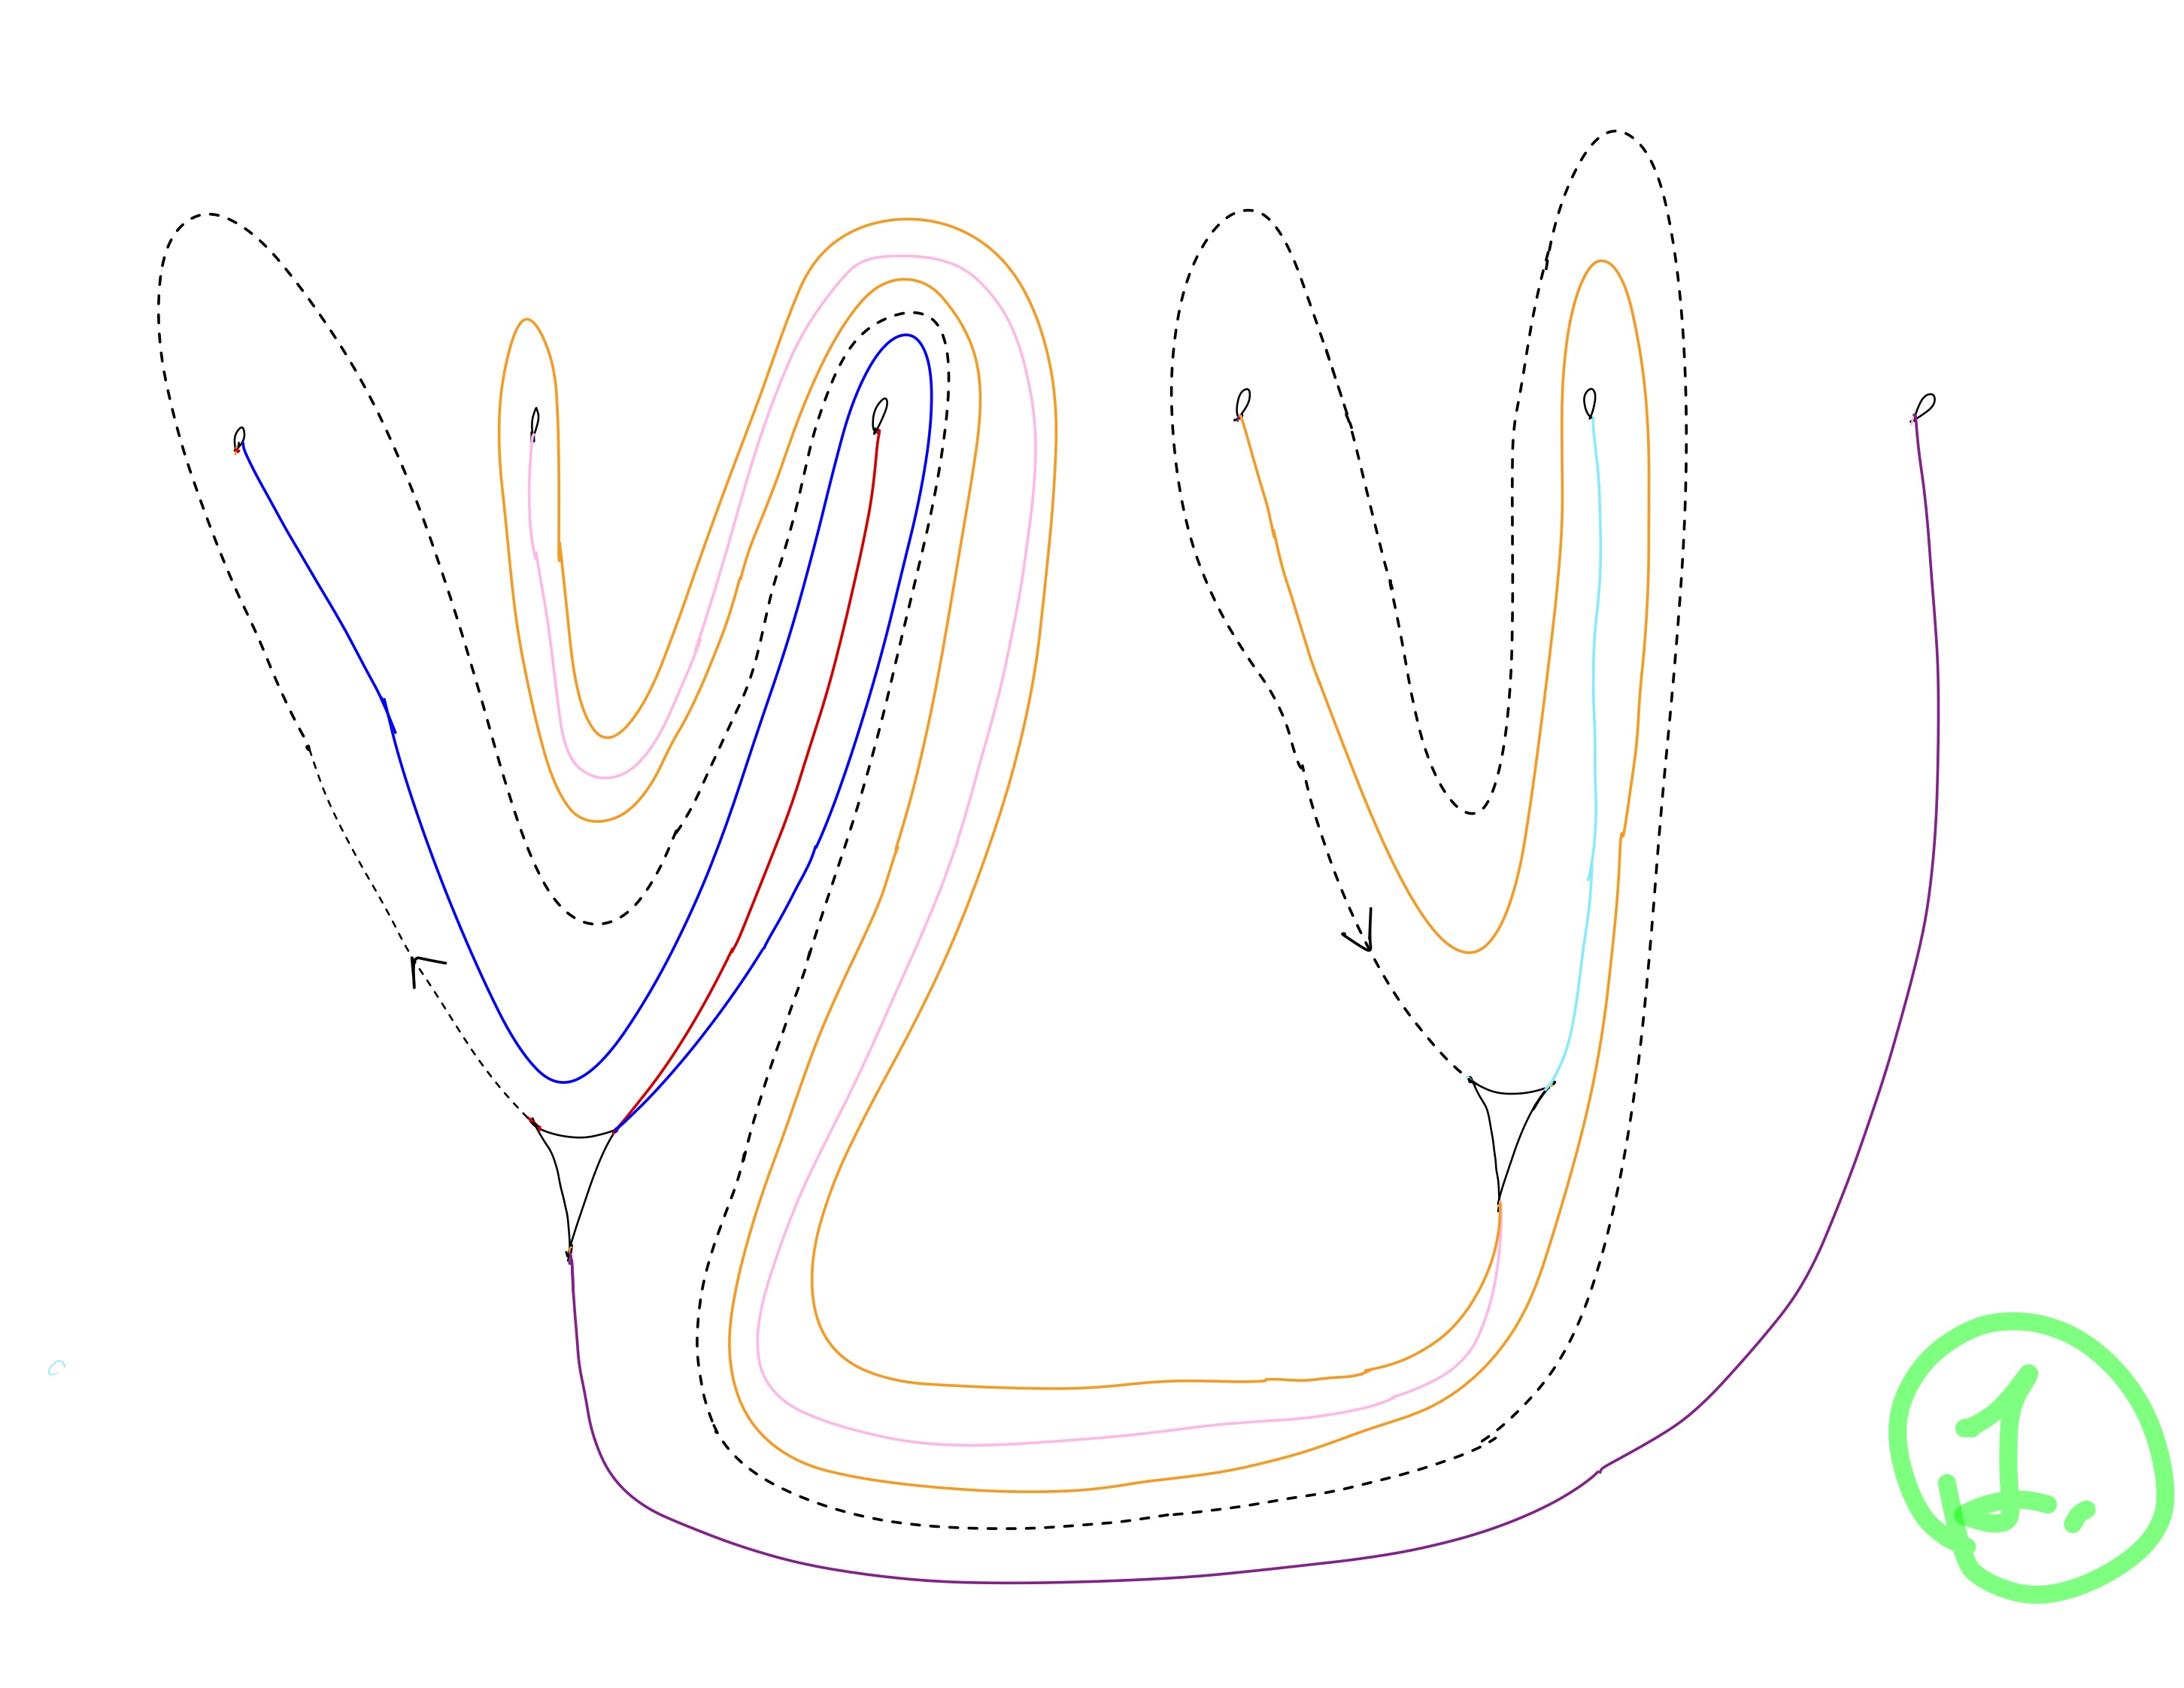
\includegraphics[width=\linewidth, height=0.45\textheight, keepaspectratio]{figures_braid/figures_track_0/Track 0 Braid 1 Loblolly-1.jpg}
    \caption{Train Track Map Candidate Family 1 of Track 0.}
    \label{fig:track0_braid_b0_1_map}
\end{figure*}

The inverse of the following braid carries this family of train track maps:
\[
b_1^0 = \sigma_{2}^{-1} \sigma_{4}^{-1} \sigma_{1}^{-1} \sigma_{3} \sigma_{2} \sigma_{1} \sigma_{3} \sigma_{2} \sigma_{3} \sigma_{2} \sigma_{1} \sigma_{4} \sigma_{3} \sigma_{2} \sigma_{5} \sigma_{4} \sigma_{3}
\]

This is shown in Figure \ref{fig:track0_braid_b0_1}.

\begin{figure*}[p]
    \centering
    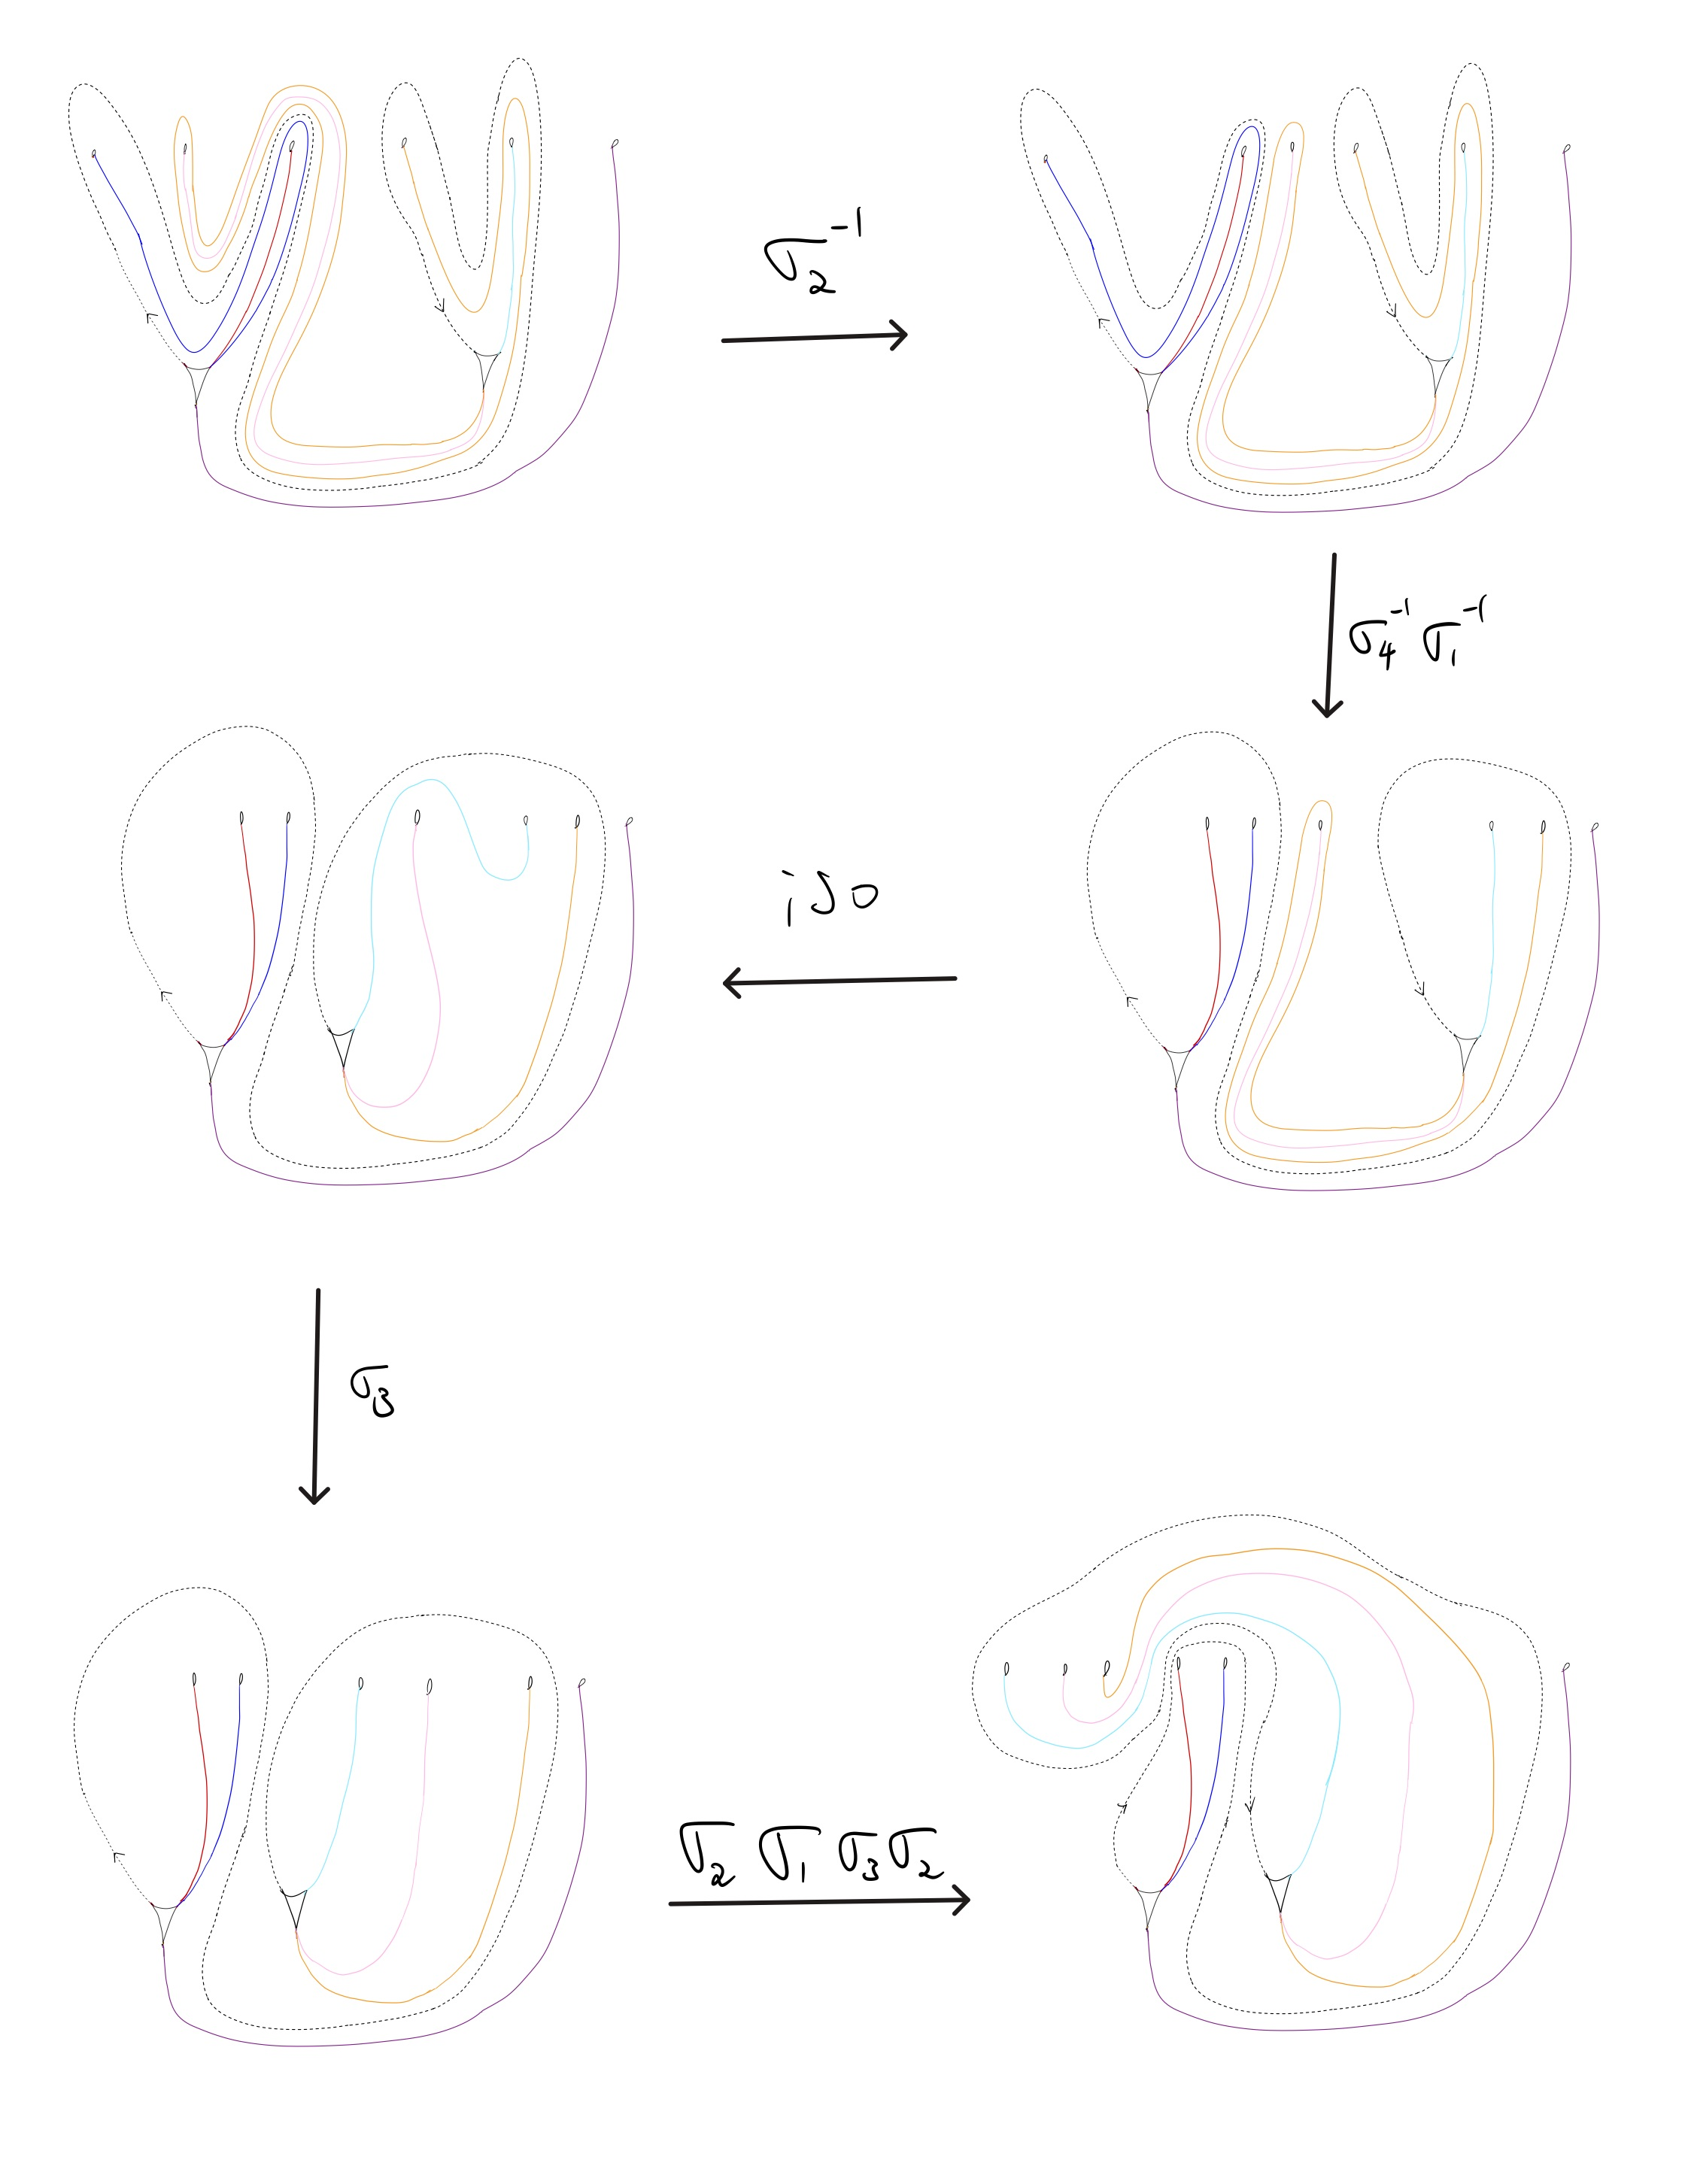
\includegraphics[width=\linewidth, height=0.45\textheight, keepaspectratio]{figures_braid/figures_track_0/Track 0 Braid 1 Loblolly-2.jpg}\\
    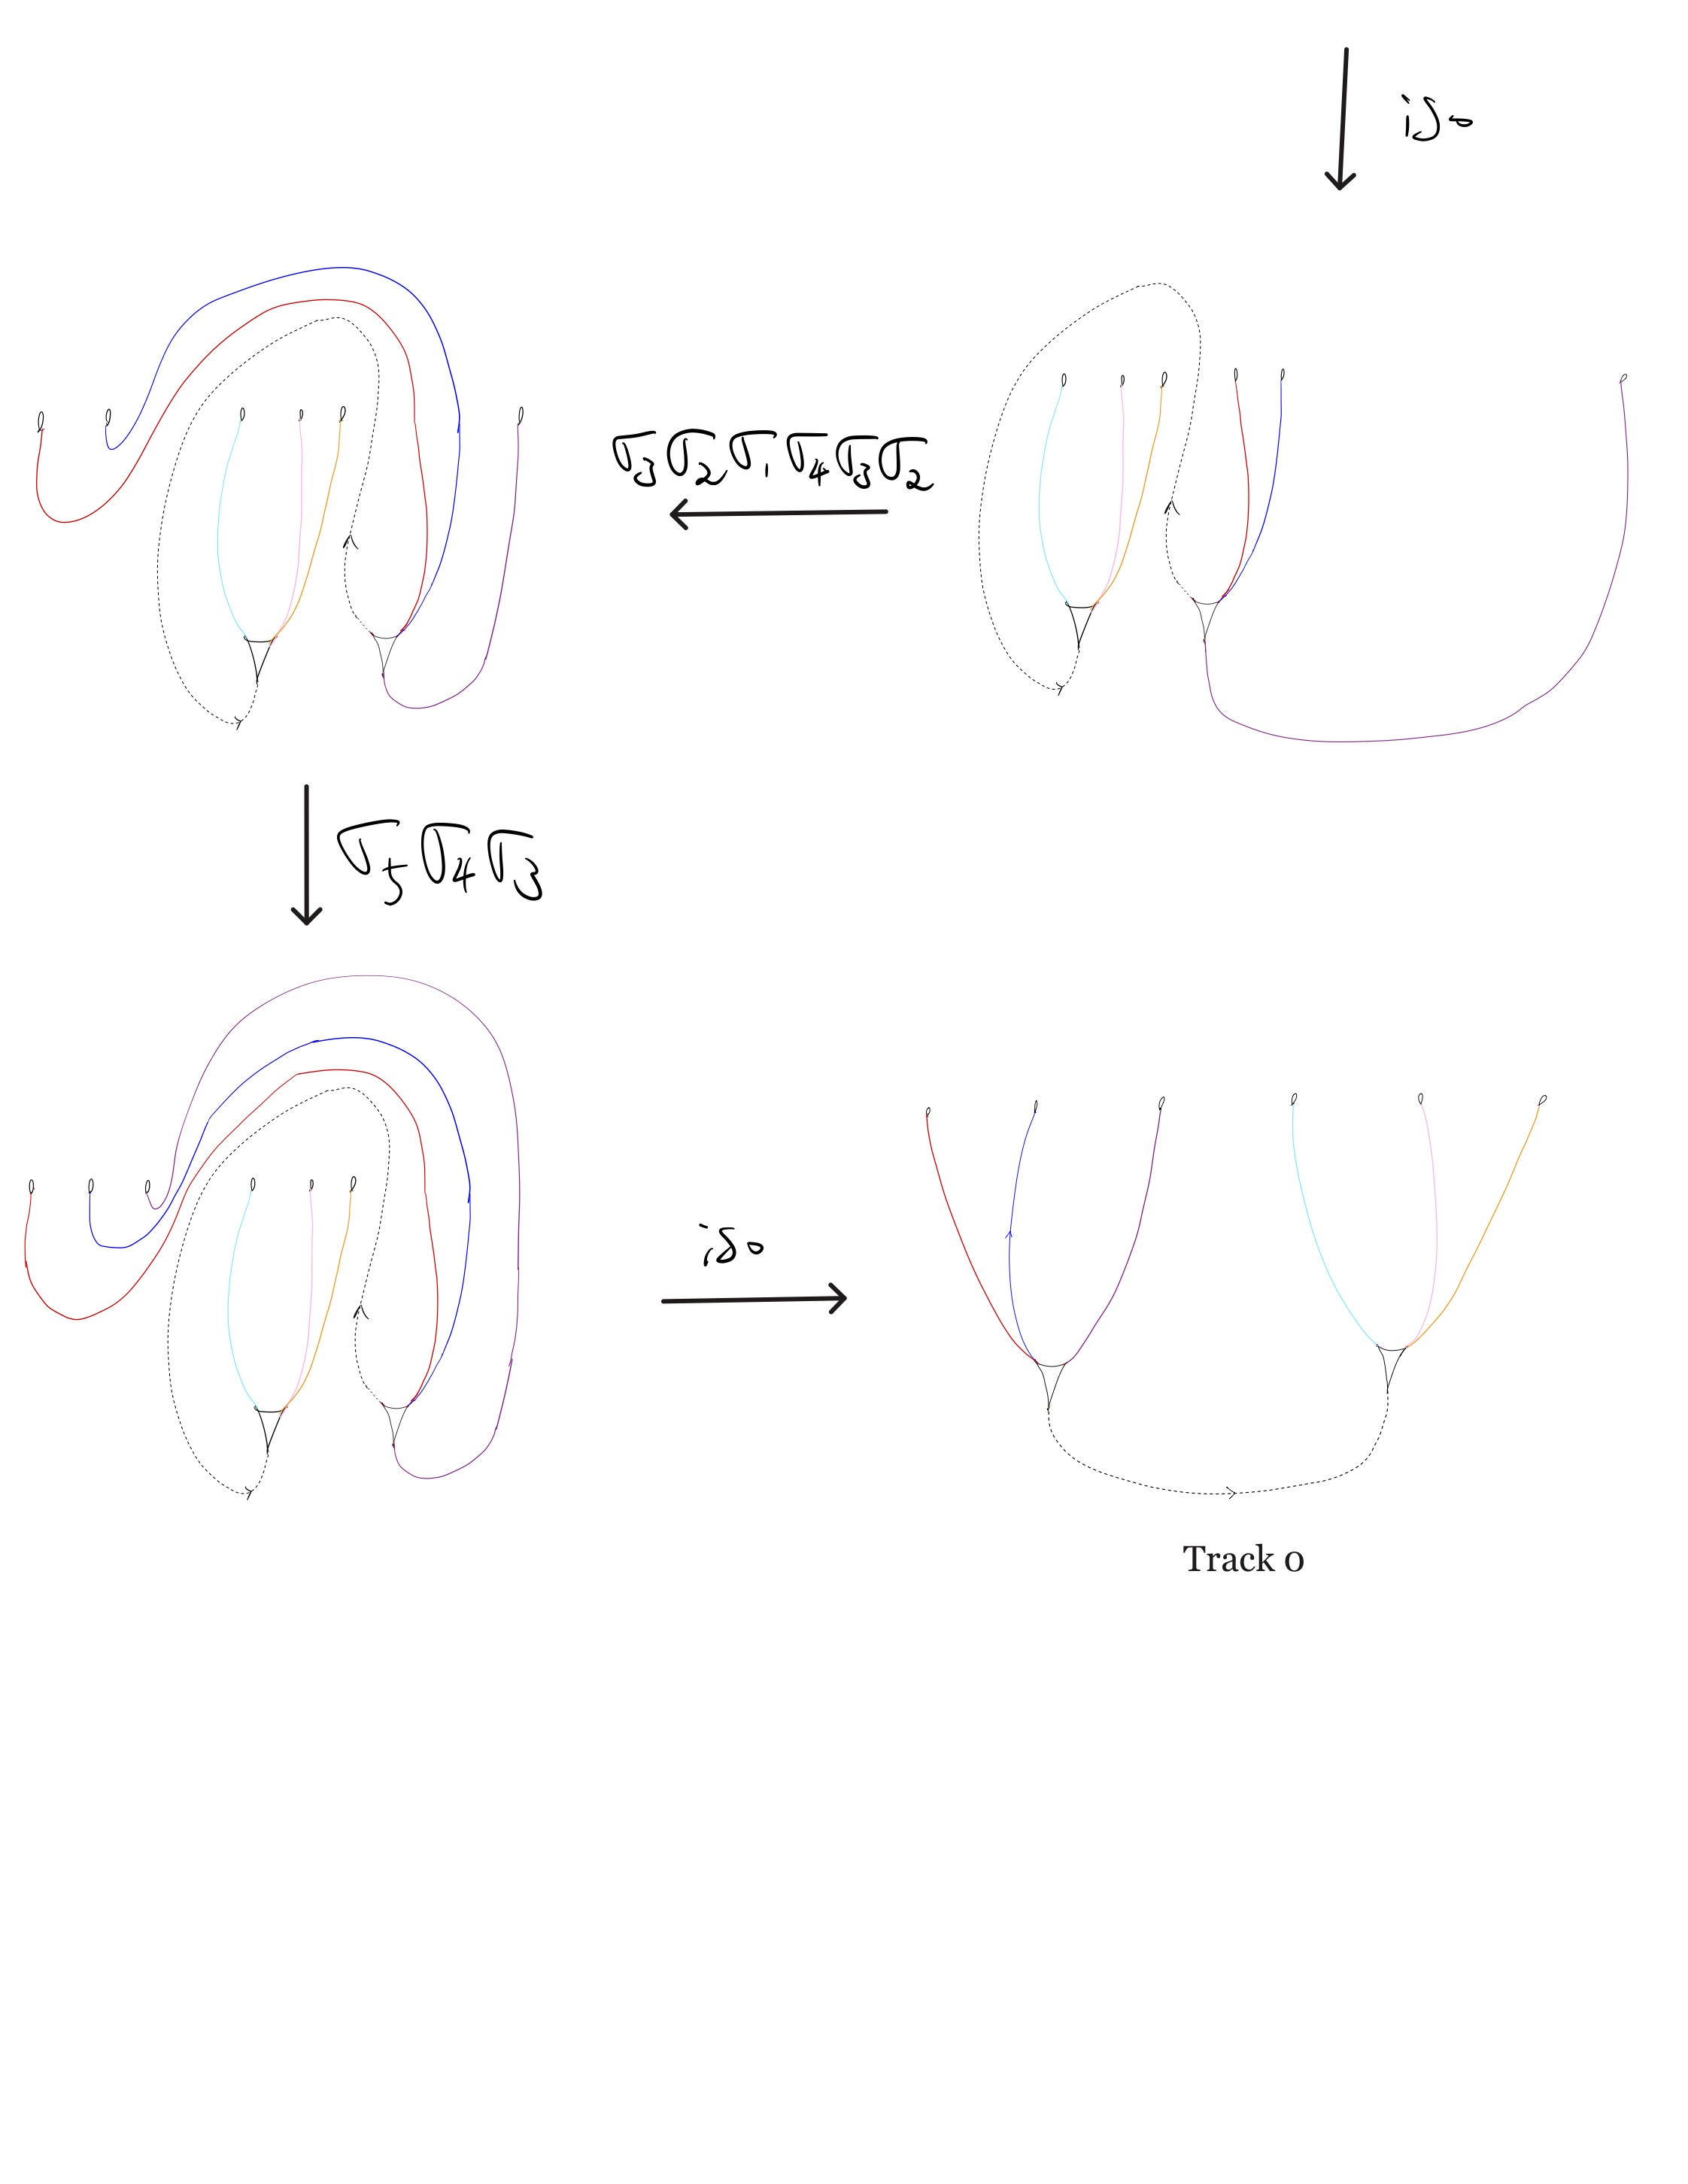
\includegraphics[width=\linewidth, height=0.45\textheight, keepaspectratio]{figures_braid/figures_track_0/Track 0 Braid 1 Loblolly-3.jpg}
    \caption{This sequence shows the inverse of the braid $b_1^0$ carries Train Track Candidate Family 1.}
    \label{fig:track0_braid_b0_1}
\end{figure*}

\clearpage

\section{Candidate Family 2 (Sloom)}\label{sec:track0_sloom}
Train Track Map Candidate Family 2 of Track 0 is shown in Figure \ref{fig:track0_braid_b0_2_map}. See \ref{Sloom} for details.

\begin{figure*}[ht]
    \centering
    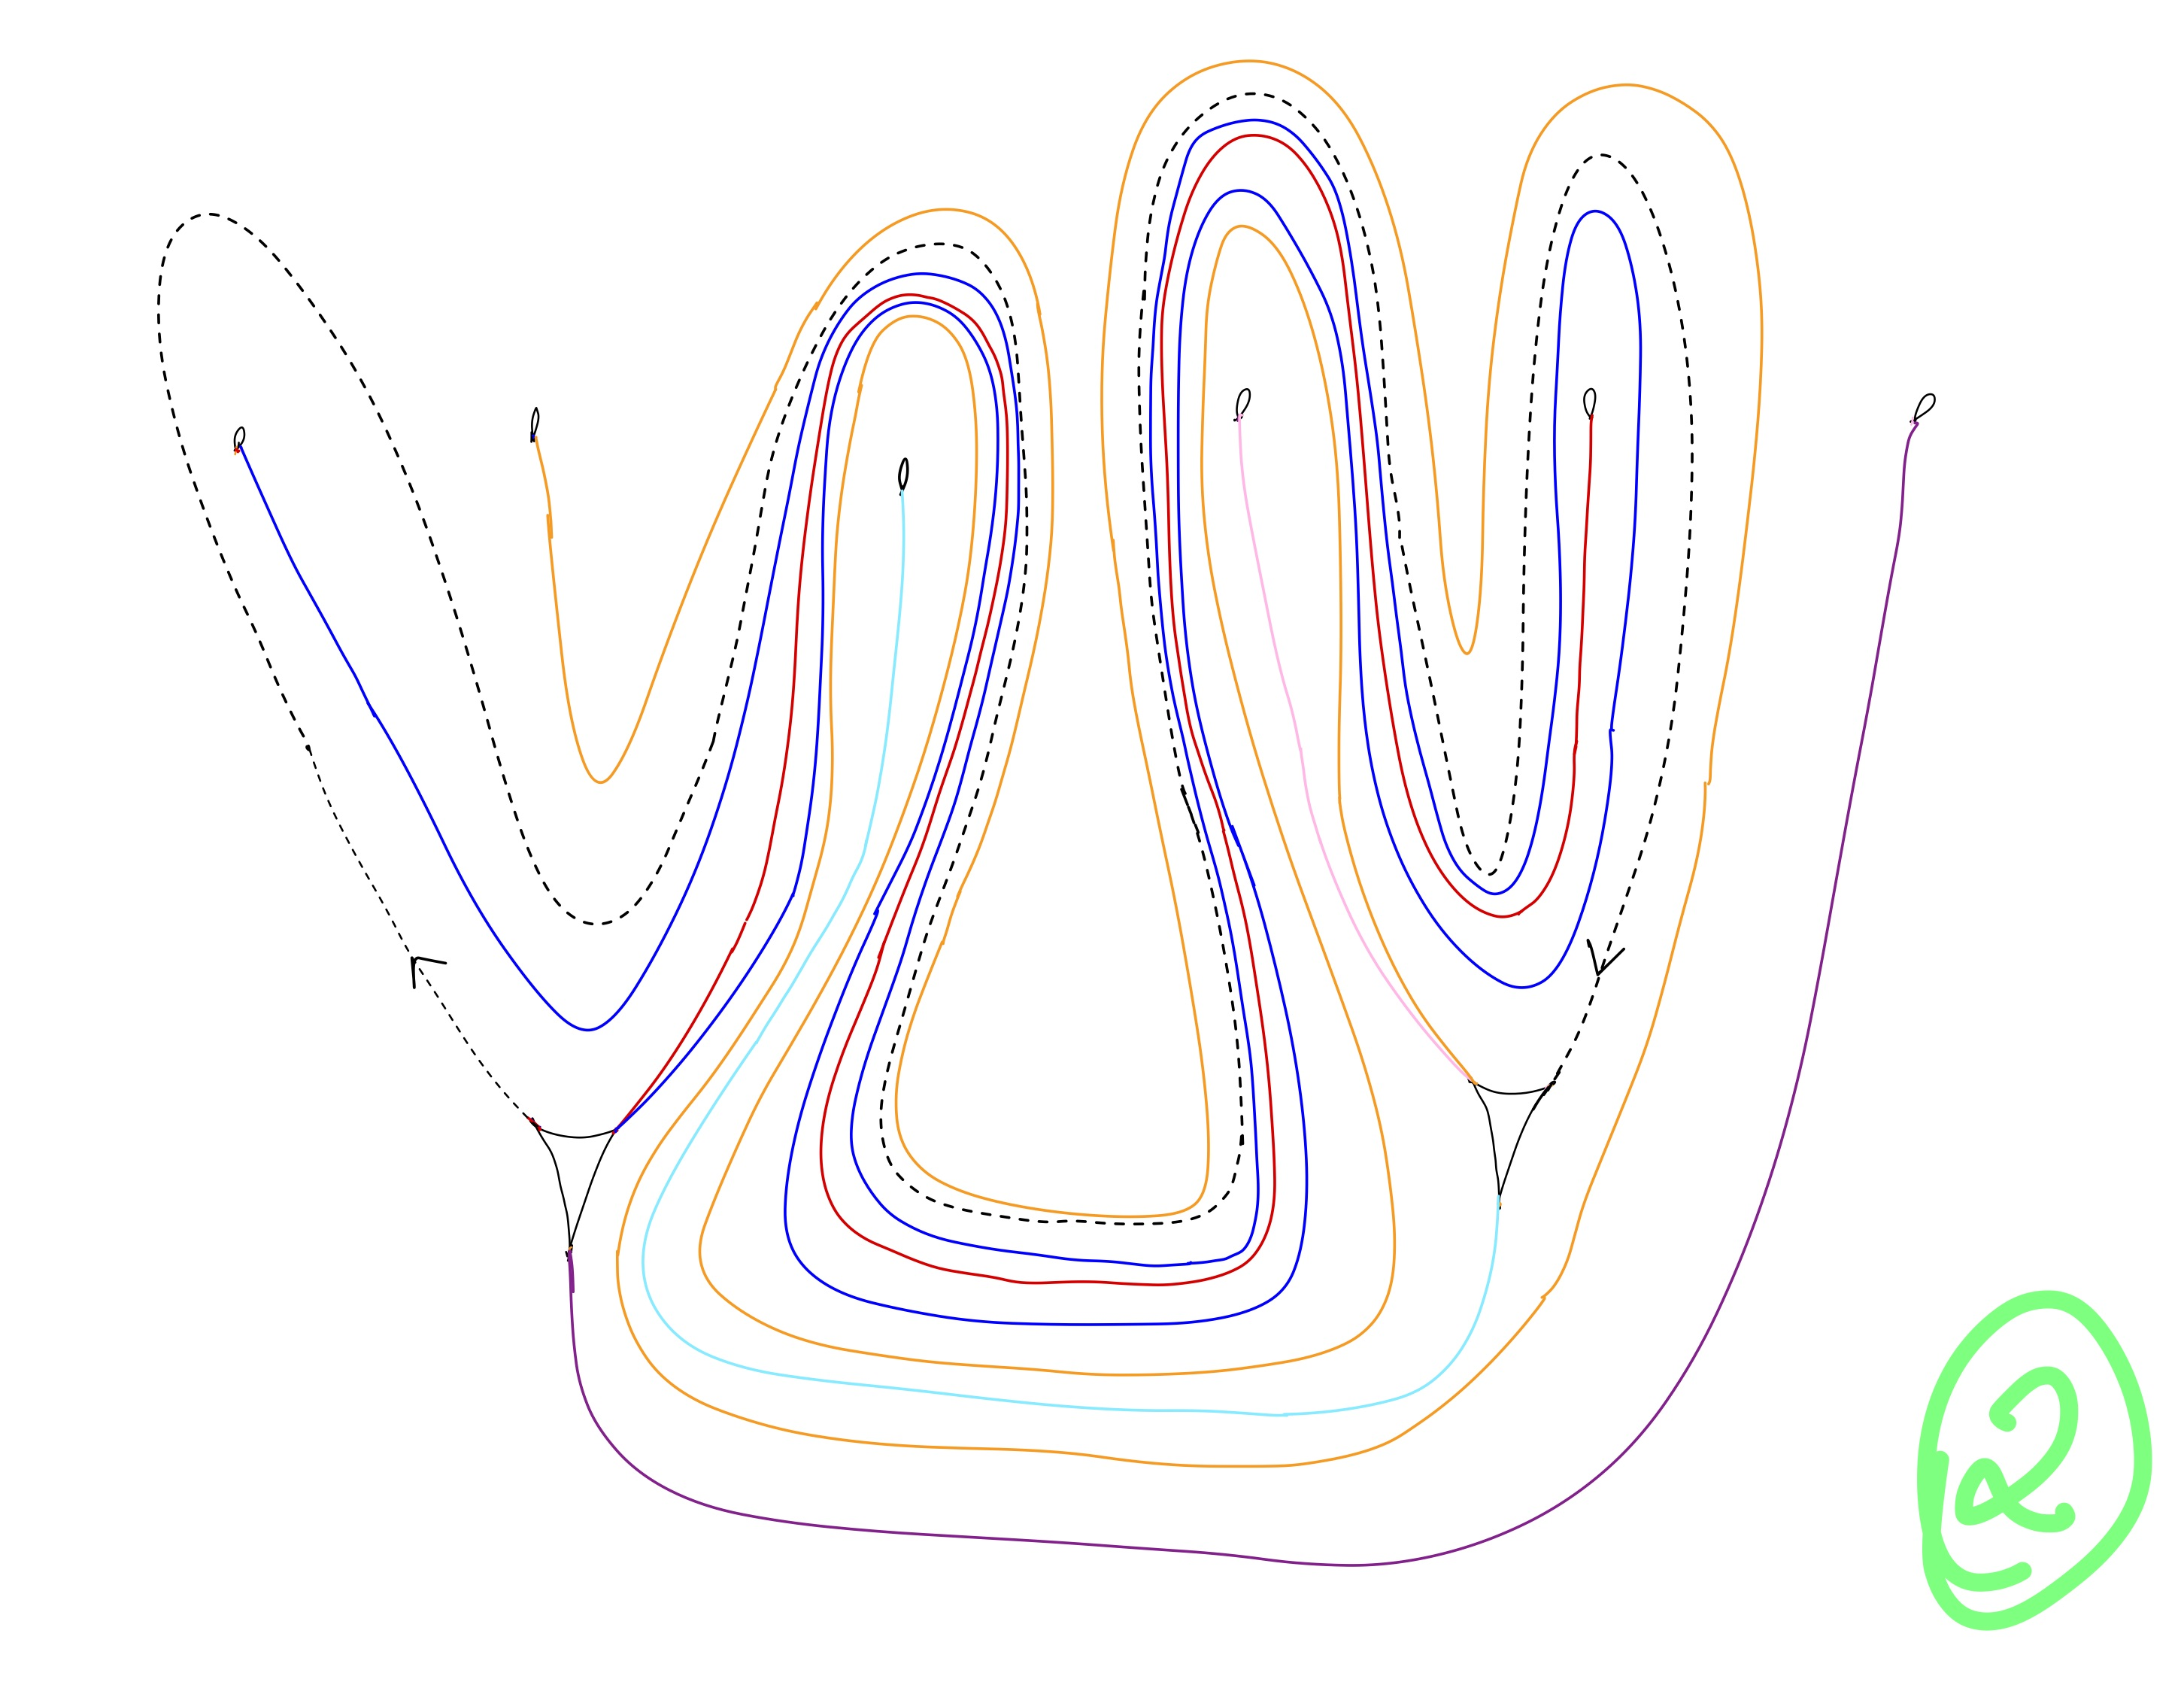
\includegraphics[width=\linewidth, height=0.45\textheight, keepaspectratio]{figures_braid/figures_track_0/Track 0 Braid 2 Sloom-1.jpg}
    \caption{Train Track Map Candidate Family 2 of Track 0.}
    \label{fig:track0_braid_b0_2_map}
\end{figure*}

The inverse of the following braid carries this family of train track maps:
\[
b_2^0 = \sigma_{2}^{-1} \sigma_{3}^{-1} \sigma_{4}^{-1} \sigma_{3} \sigma_{2} \sigma_{1}^{-1} \sigma_{4} \sigma_{3} \sigma_{2} \sigma_{1} \sigma_{2} \sigma_{1} \sigma_{3} \sigma_{2} \sigma_{1}^{-1} \sigma_{2}^{-1} \sigma_{3}^{-1} \sigma_{1} \sigma_{1} \cdot J \cdot \Lambda_6
\]

This is shown in Figure \ref{fig:track0_braid_b0_2}.

\begin{figure*}[p]
    \centering
    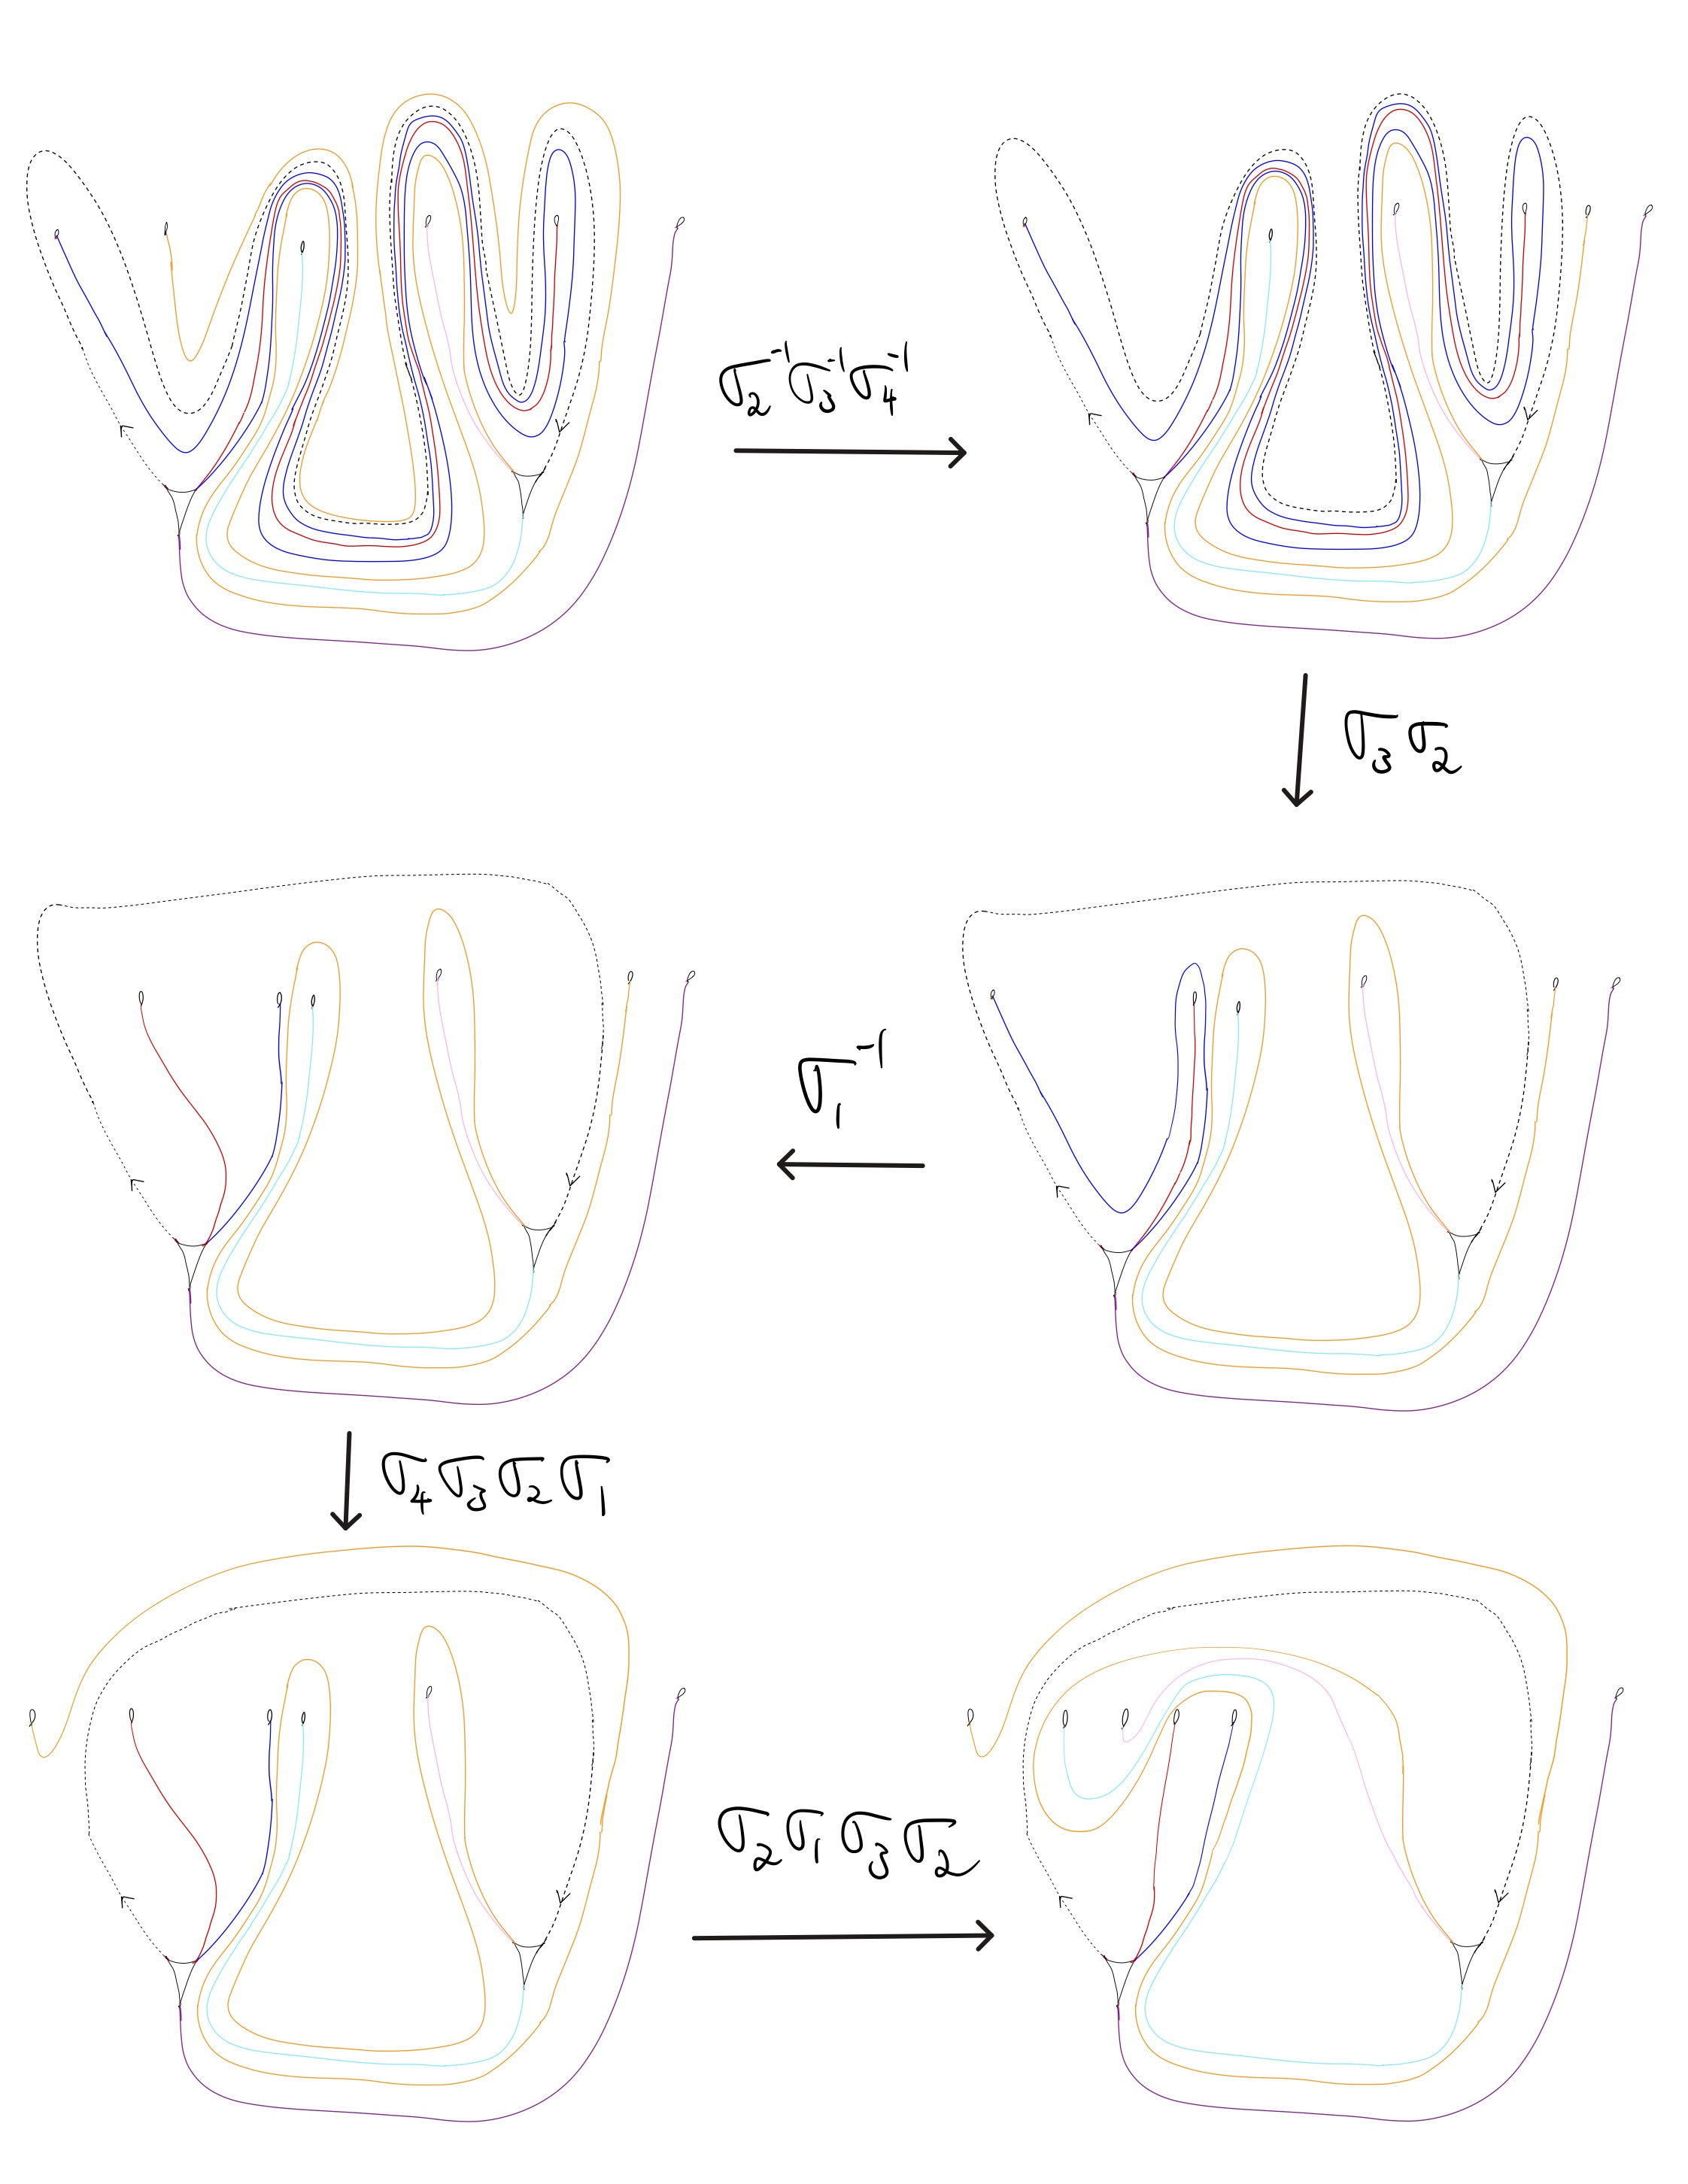
\includegraphics[width=\linewidth, height=0.45\textheight, keepaspectratio]{figures_braid/figures_track_0/Track 0 Braid 2 Sloom-2.jpg}\\
    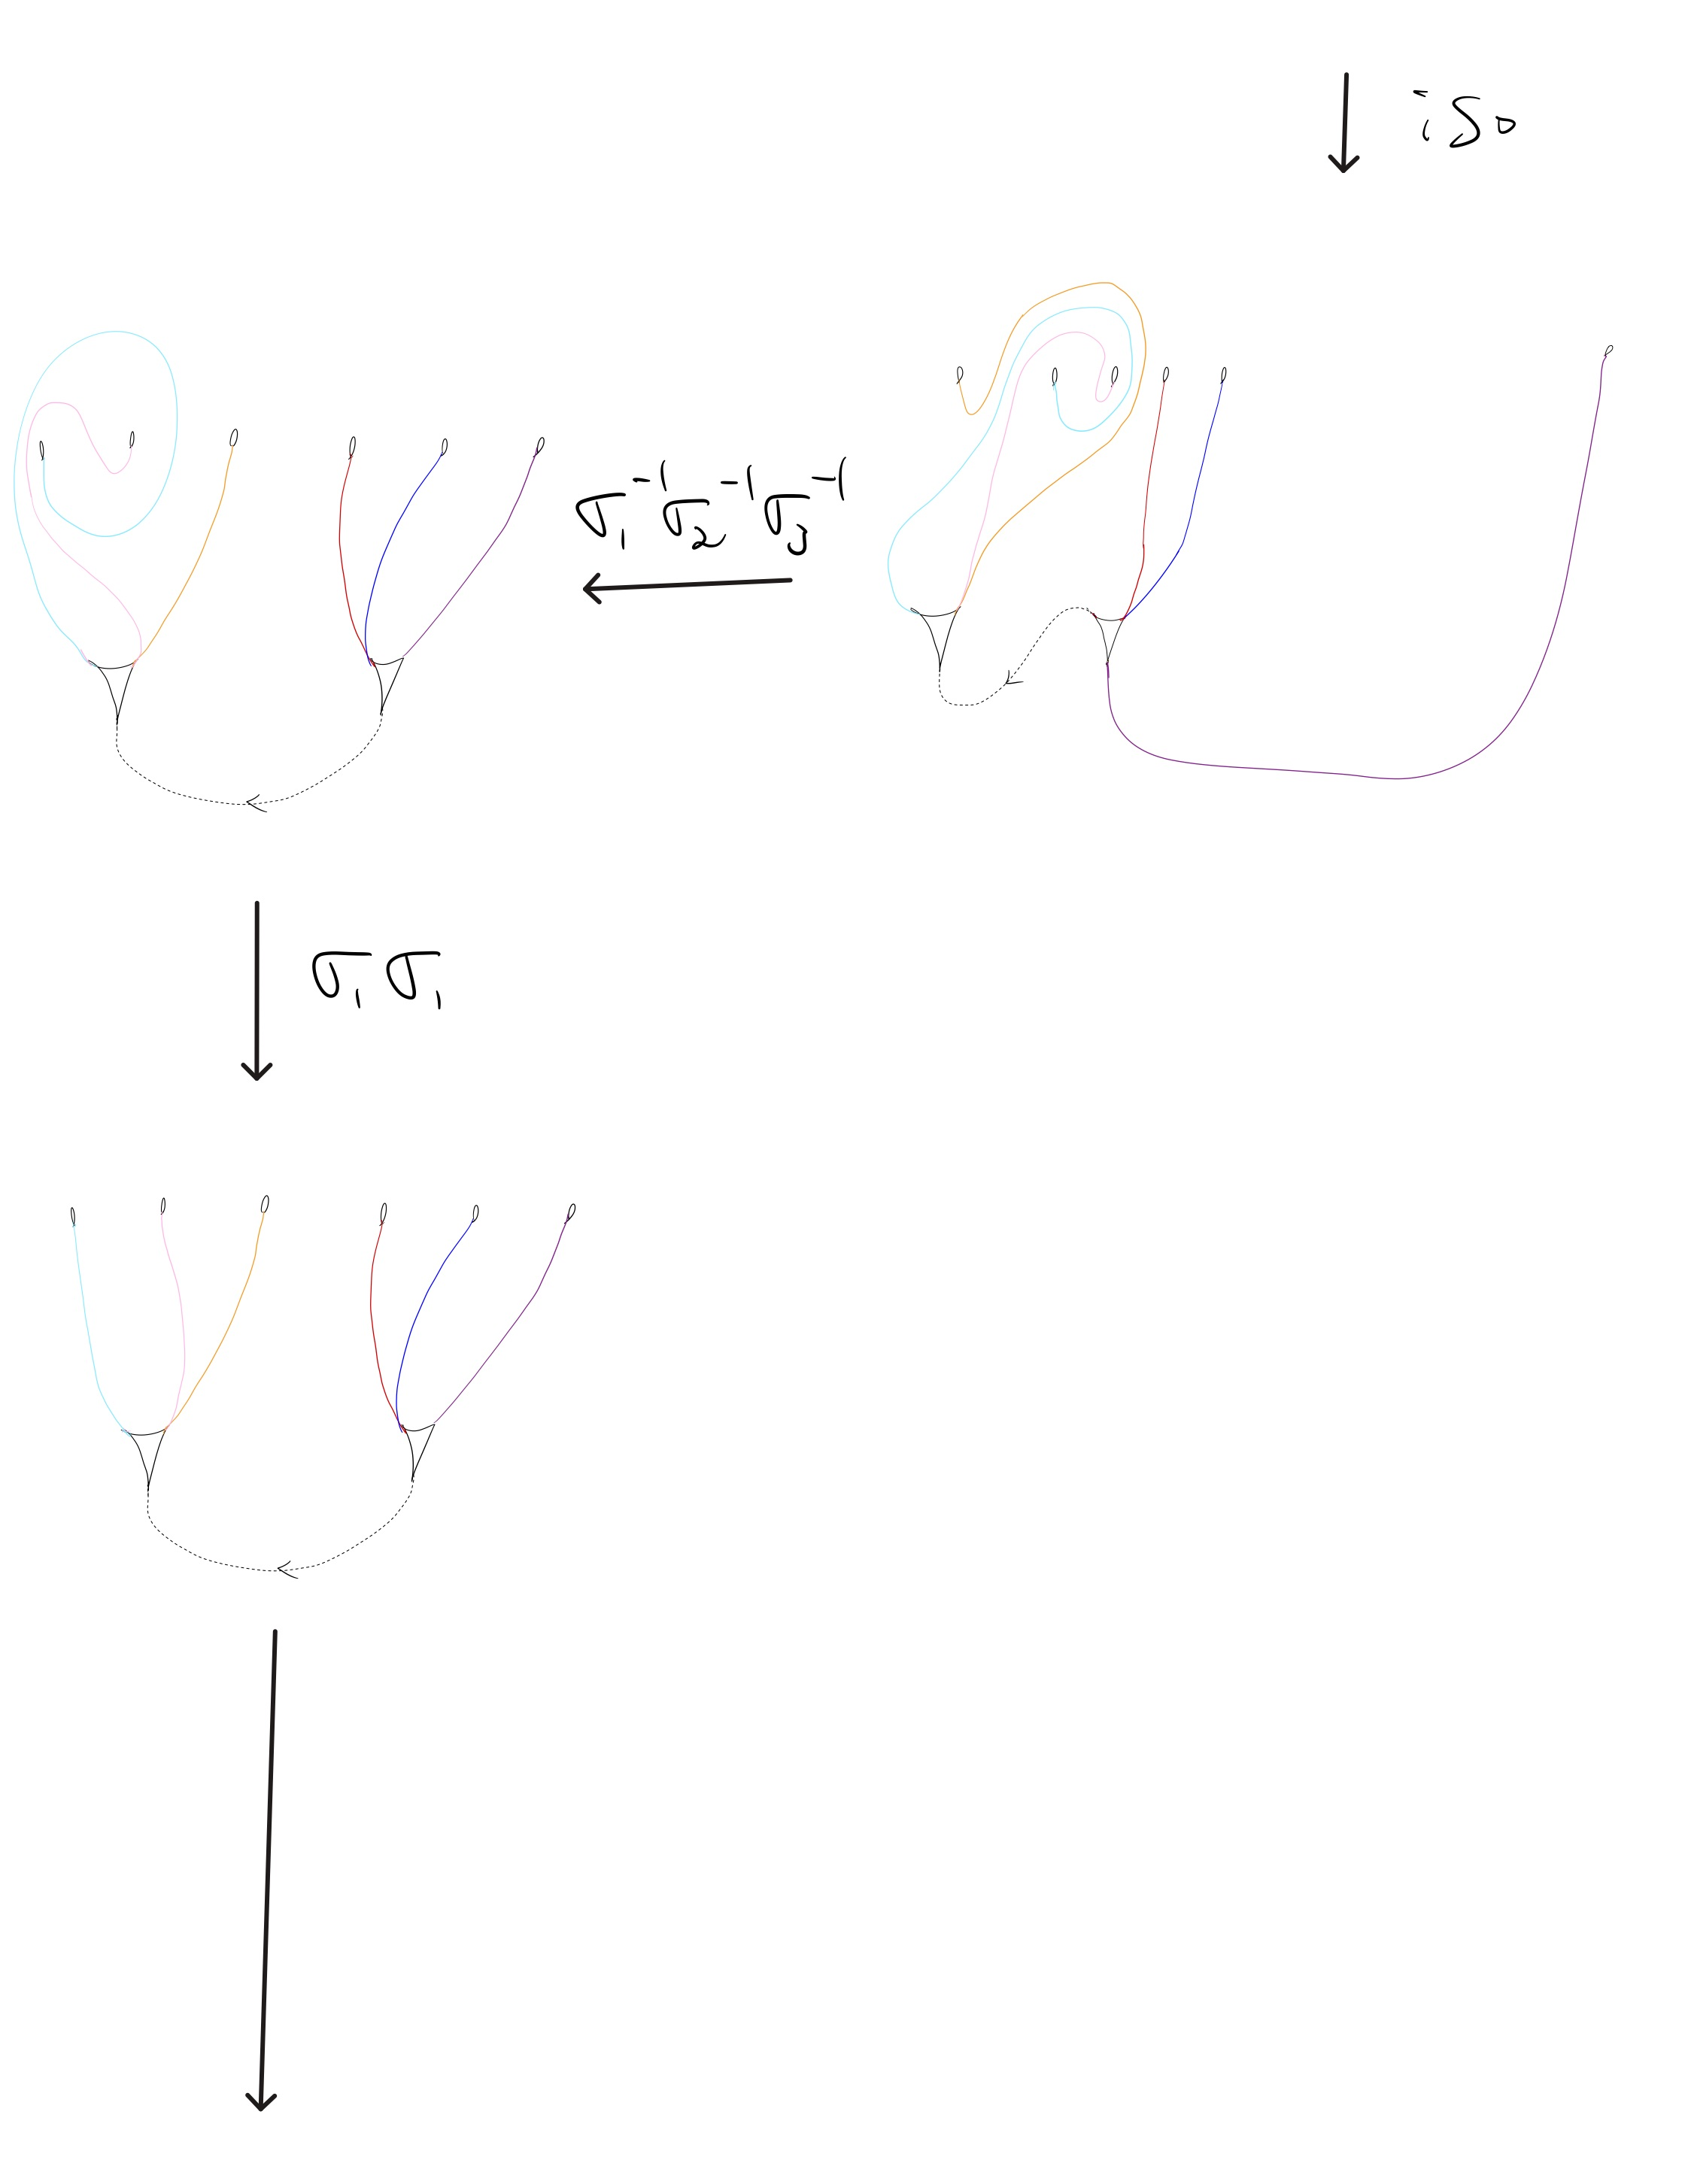
\includegraphics[width=\linewidth, height=0.45\textheight, keepaspectratio]{figures_braid/figures_track_0/Track 0 Braid 2 Sloom-3.jpg}
    \caption{This sequence shows the inverse of the braid $b_2^0$ carries Train Track Candidate Family 2.}
    \label{fig:track0_braid_b0_2}
\end{figure*}

\begin{figure*}[p]
    \ContinuedFloat
    \centering
    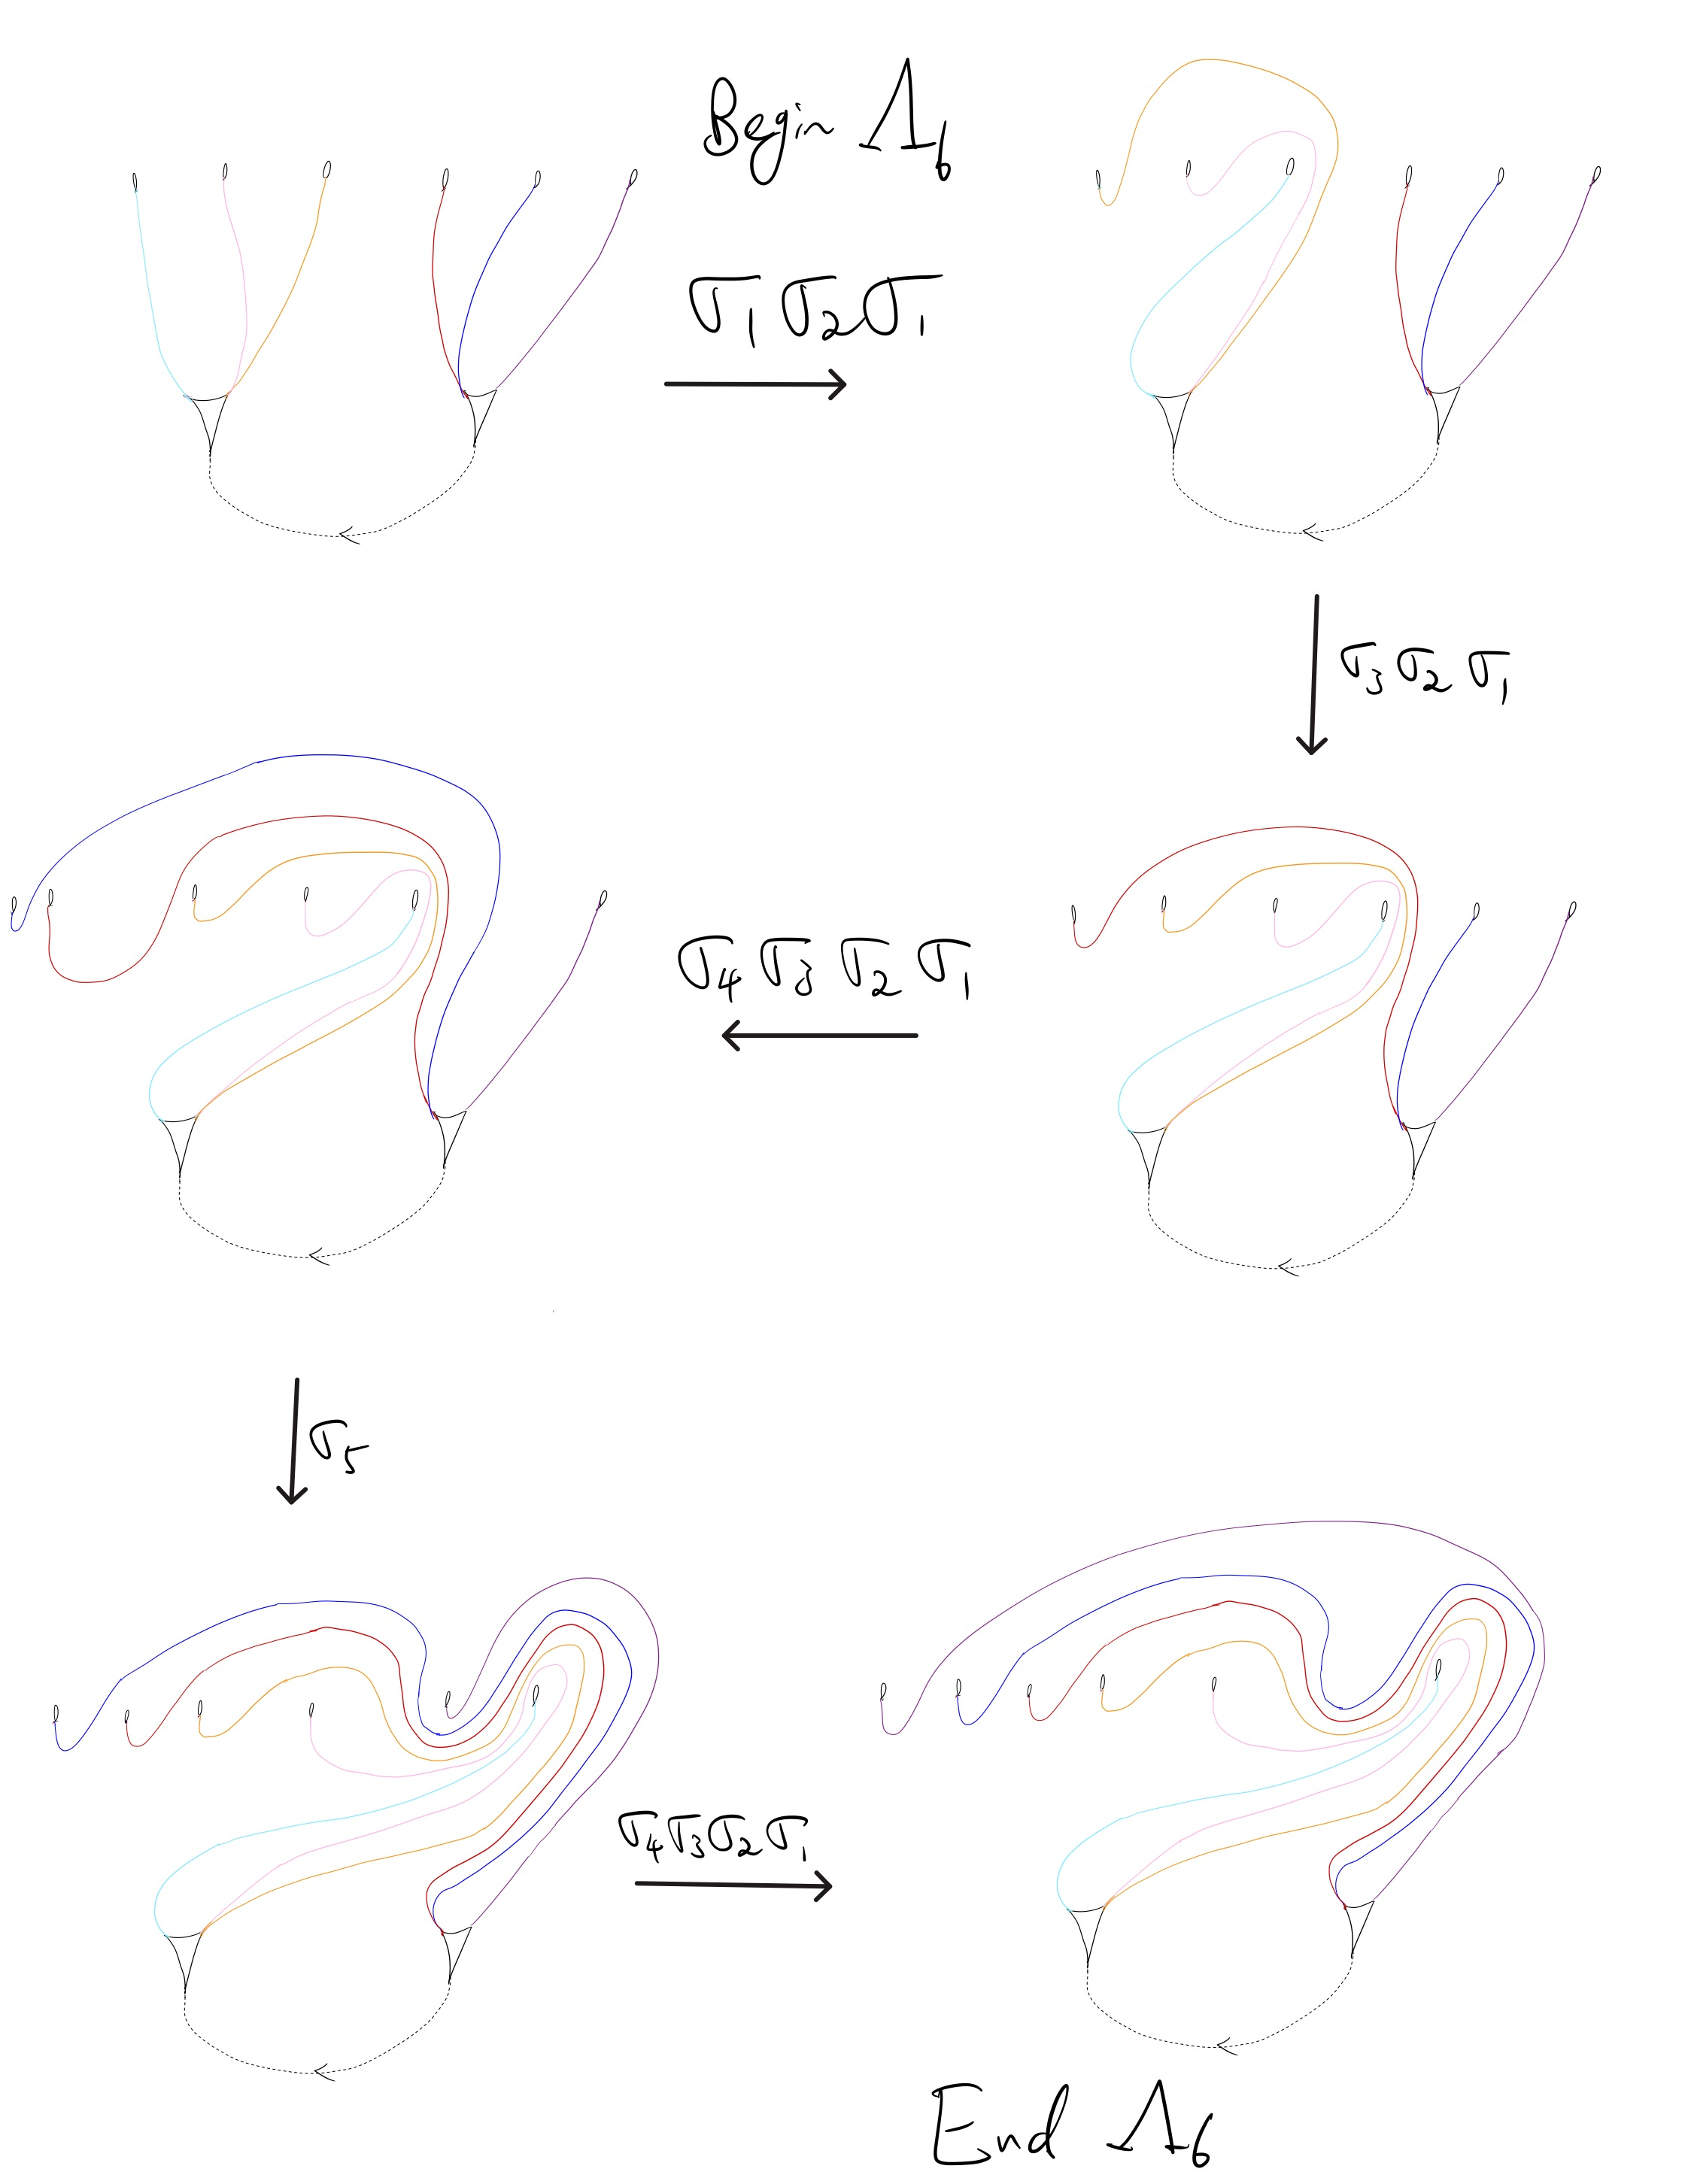
\includegraphics[width=\linewidth, height=0.45\textheight, keepaspectratio]{figures_braid/figures_track_0/Track 0 Braid 2 Sloom-4.jpg}\\
    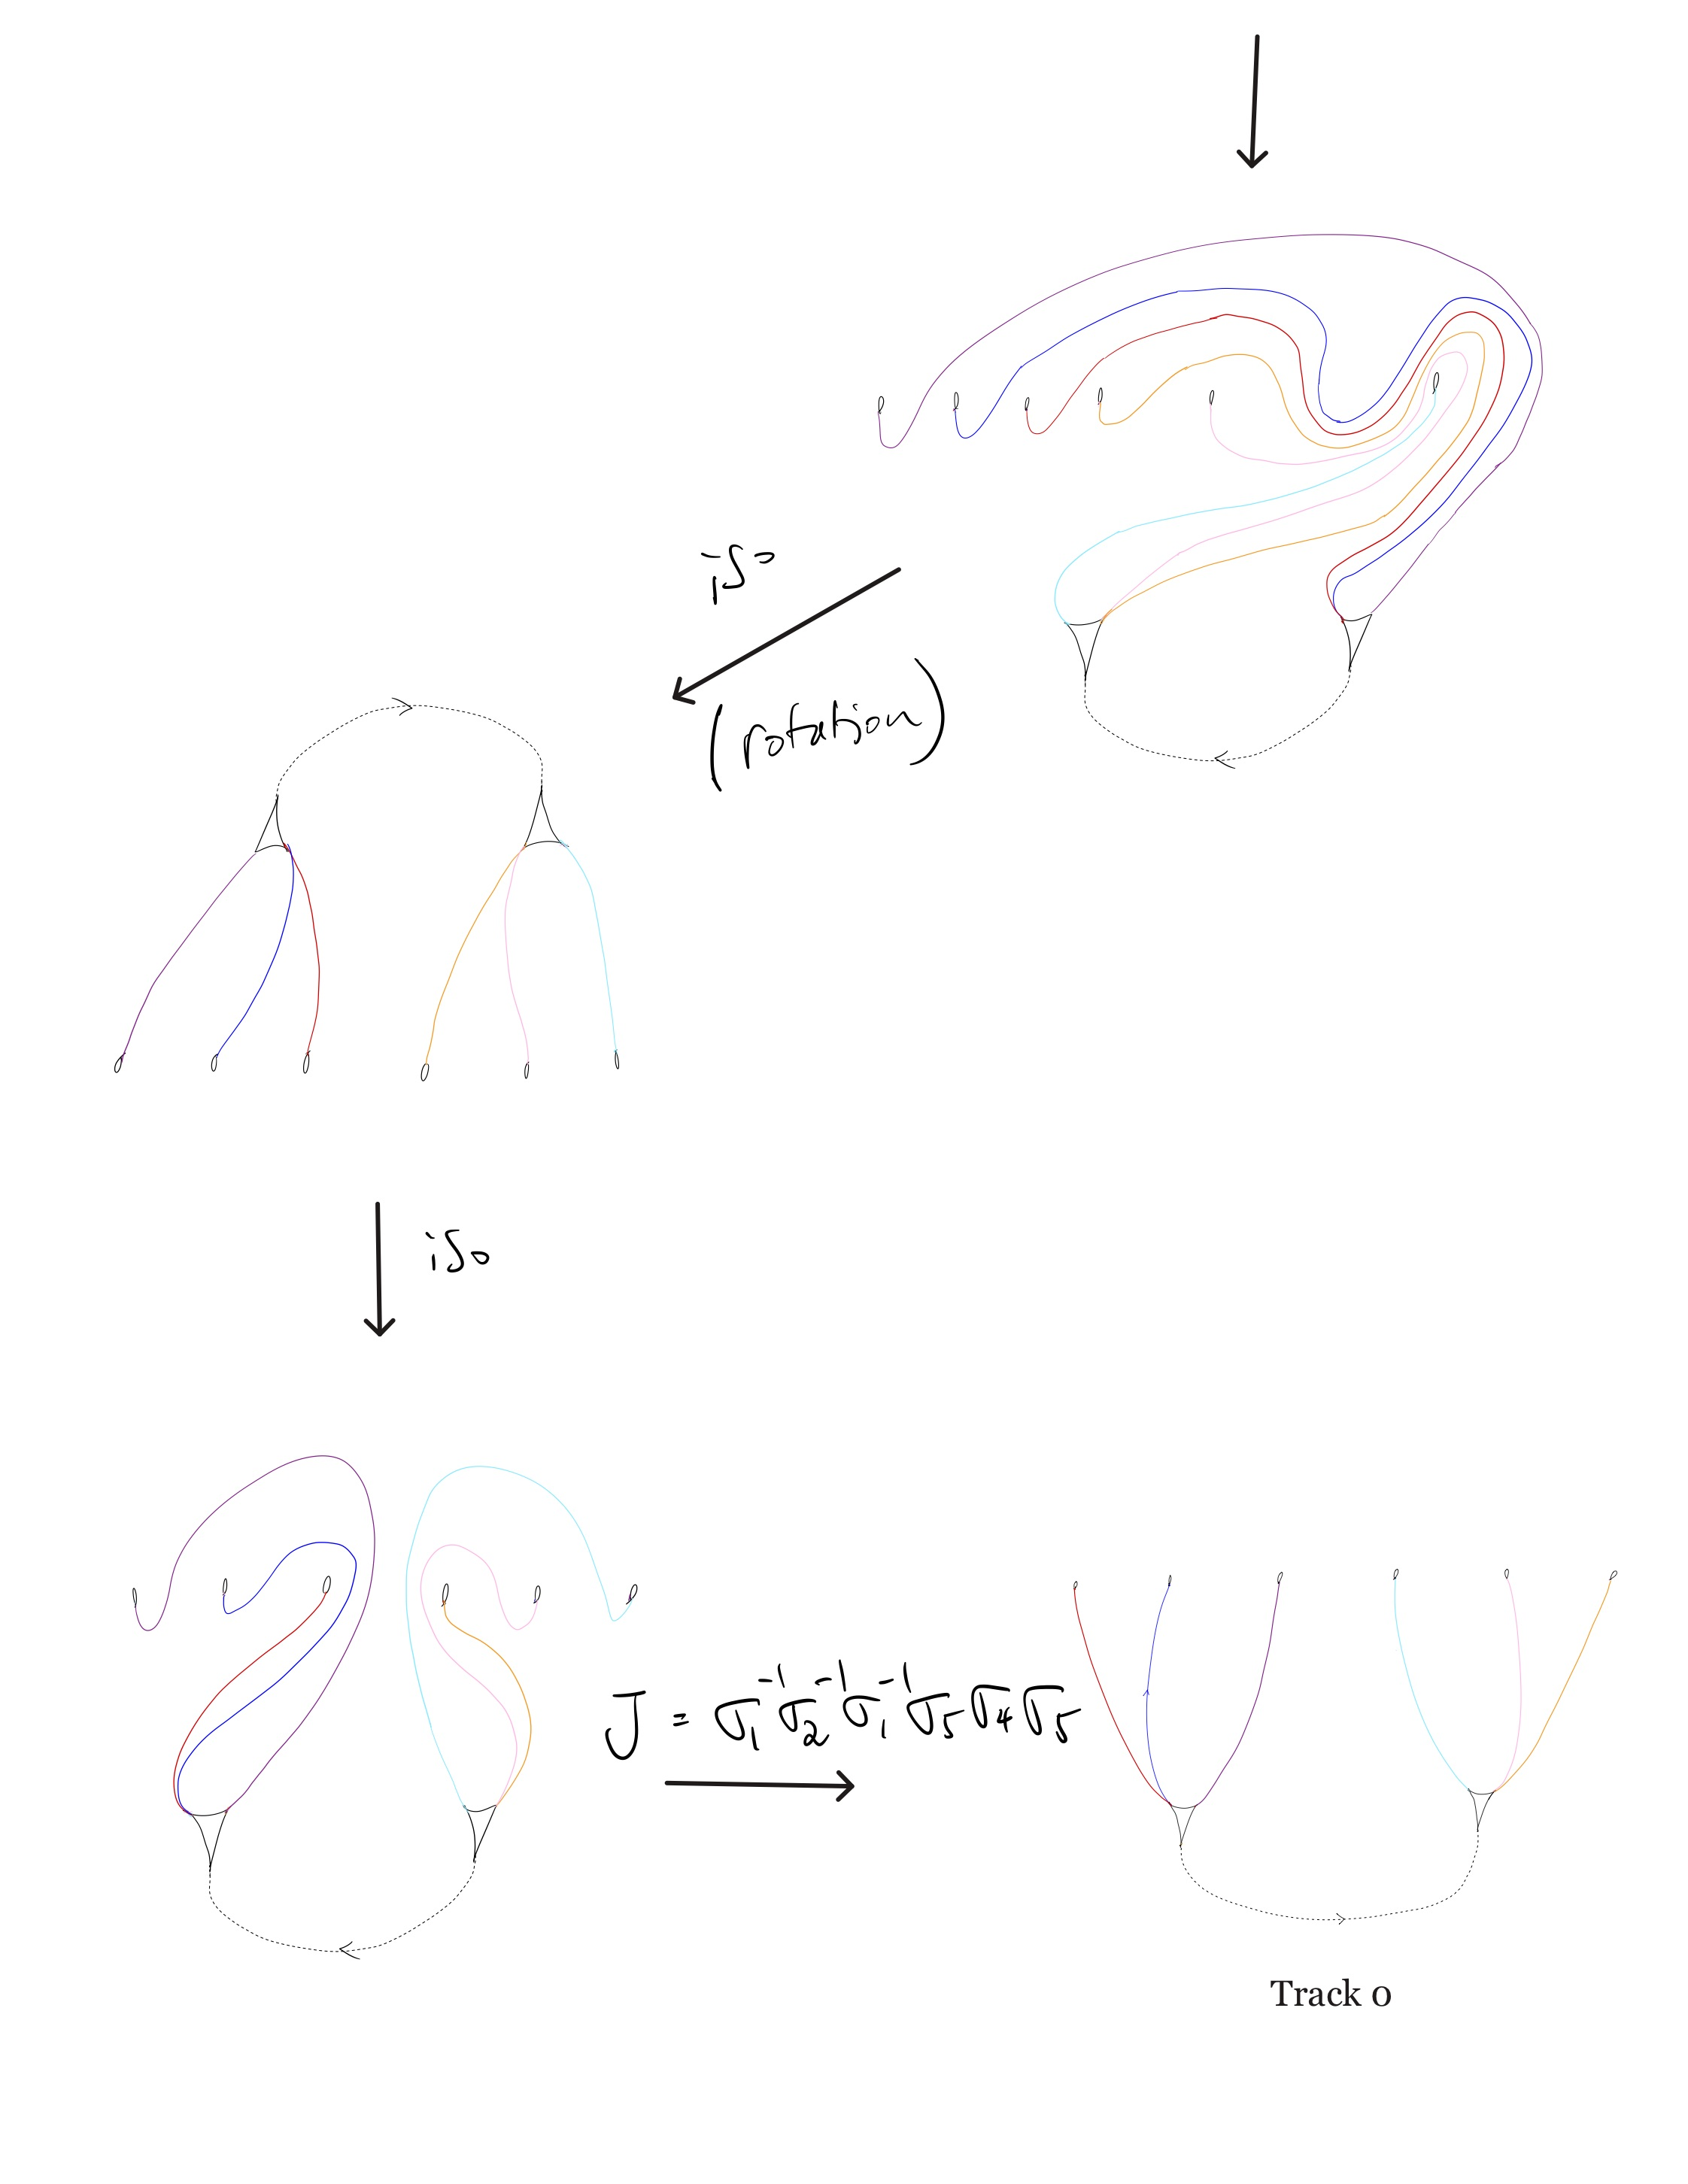
\includegraphics[width=\linewidth, height=0.45\textheight, keepaspectratio]{figures_braid/figures_track_0/Track 0 Braid 2 Sloom-5.jpg}
    \caption[]{This sequence shows the inverse of the braid $b_2^0$ carries Train Track Candidate Family 2 (continued).}
\end{figure*}

\clearpage

\section{Candidate Family 3 (Mooncalf)}\label{sec:track0_mooncalf}
Train Track Map Candidate Family 3 of Track 0 is shown in Figure \ref{fig:track0_braid_b0_3_map}. See \ref{Mooncalf} for details.

\begin{figure*}[ht]
    \centering
    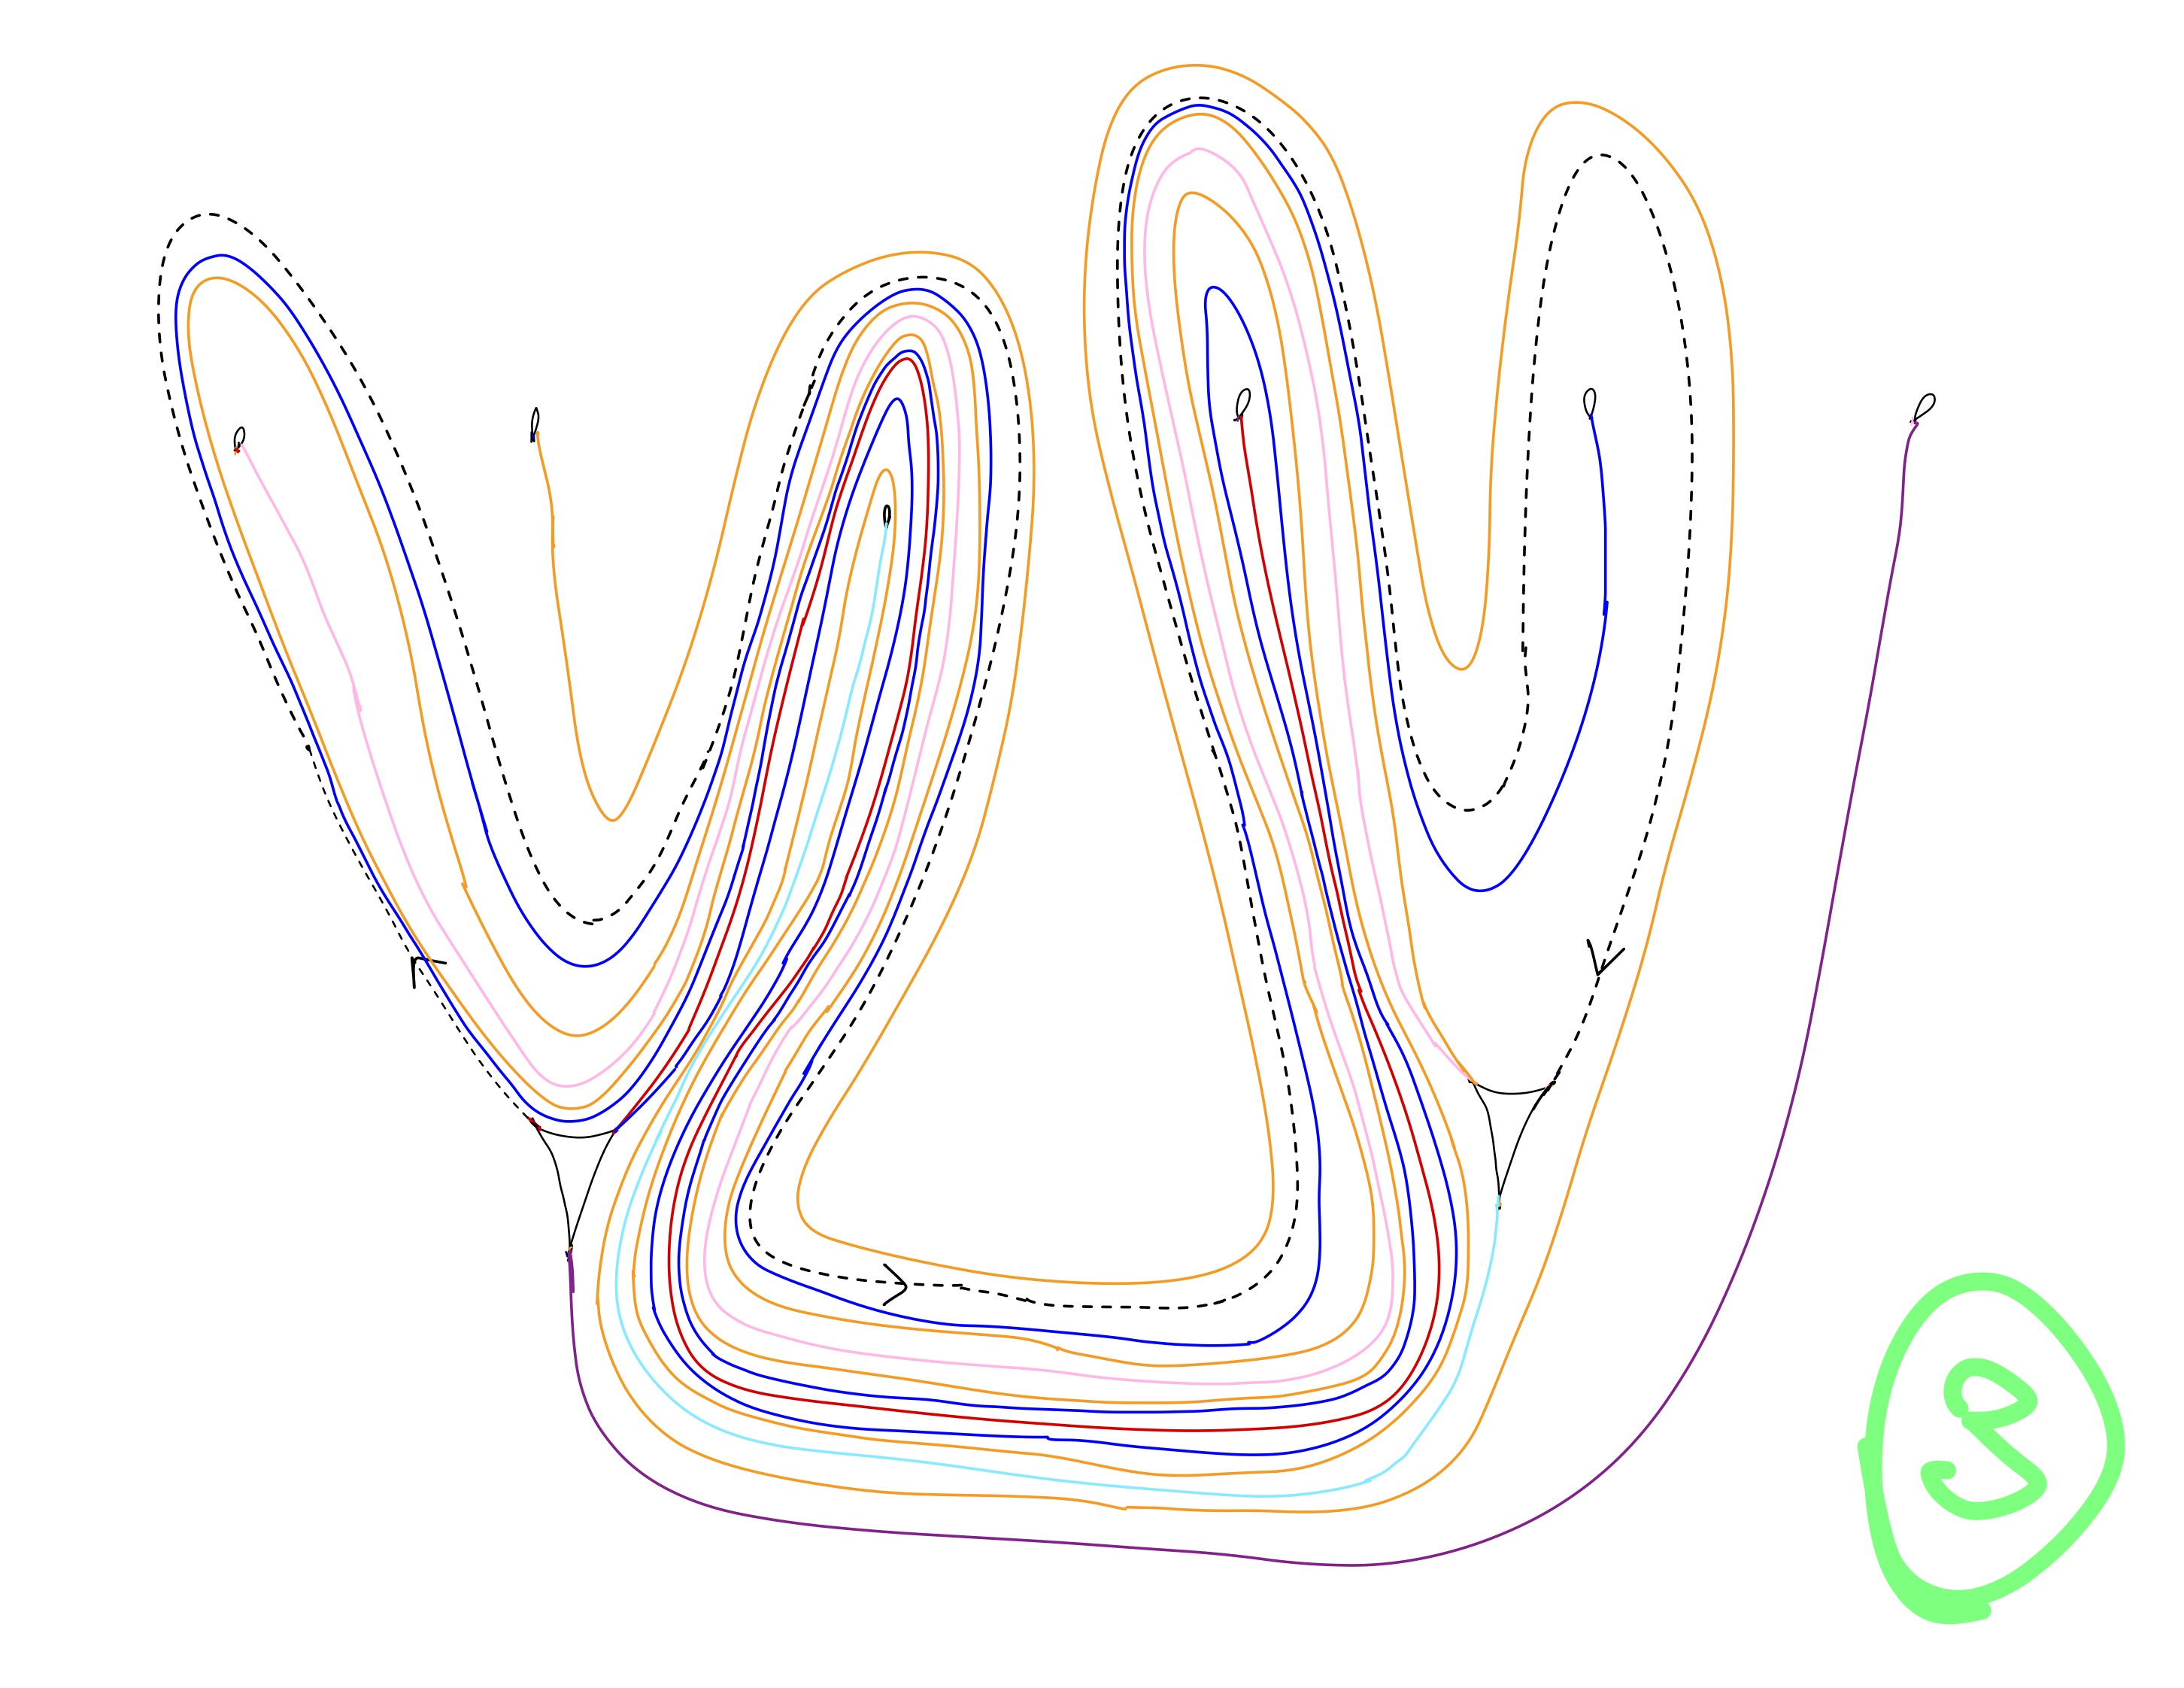
\includegraphics[width=\linewidth, height=0.45\textheight, keepaspectratio]{figures_braid/figures_track_0/Track 0 Braid 3 Mooncalf-1.jpg}
    \caption{Train Track Map Candidate Family 3 of Track 0.}
    \label{fig:track0_braid_b0_3_map}
\end{figure*}

The inverse of the following braid carries this family of train track maps:
\[
b_3^0 = \sigma_{2}^{-1} \sigma_{3}^{-1} \sigma_{4}^{-1} \sigma_{2} \sigma_{1}^{-1} \sigma_{2}^{-1} \sigma_{3} \sigma_{2} \sigma_{4}^{-1} \sigma_{3}^{-1} \sigma_{2} \sigma_{1} \sigma_{4} \sigma_{3} \sigma_{2} \sigma_{1} \sigma_{4} \sigma_{3} \sigma_{2} \sigma_{1} \cdot J \cdot \Lambda_6
\]

This is shown in Figure \ref{fig:track0_braid_b0_3}.

\begin{figure*}[p]
    \centering
    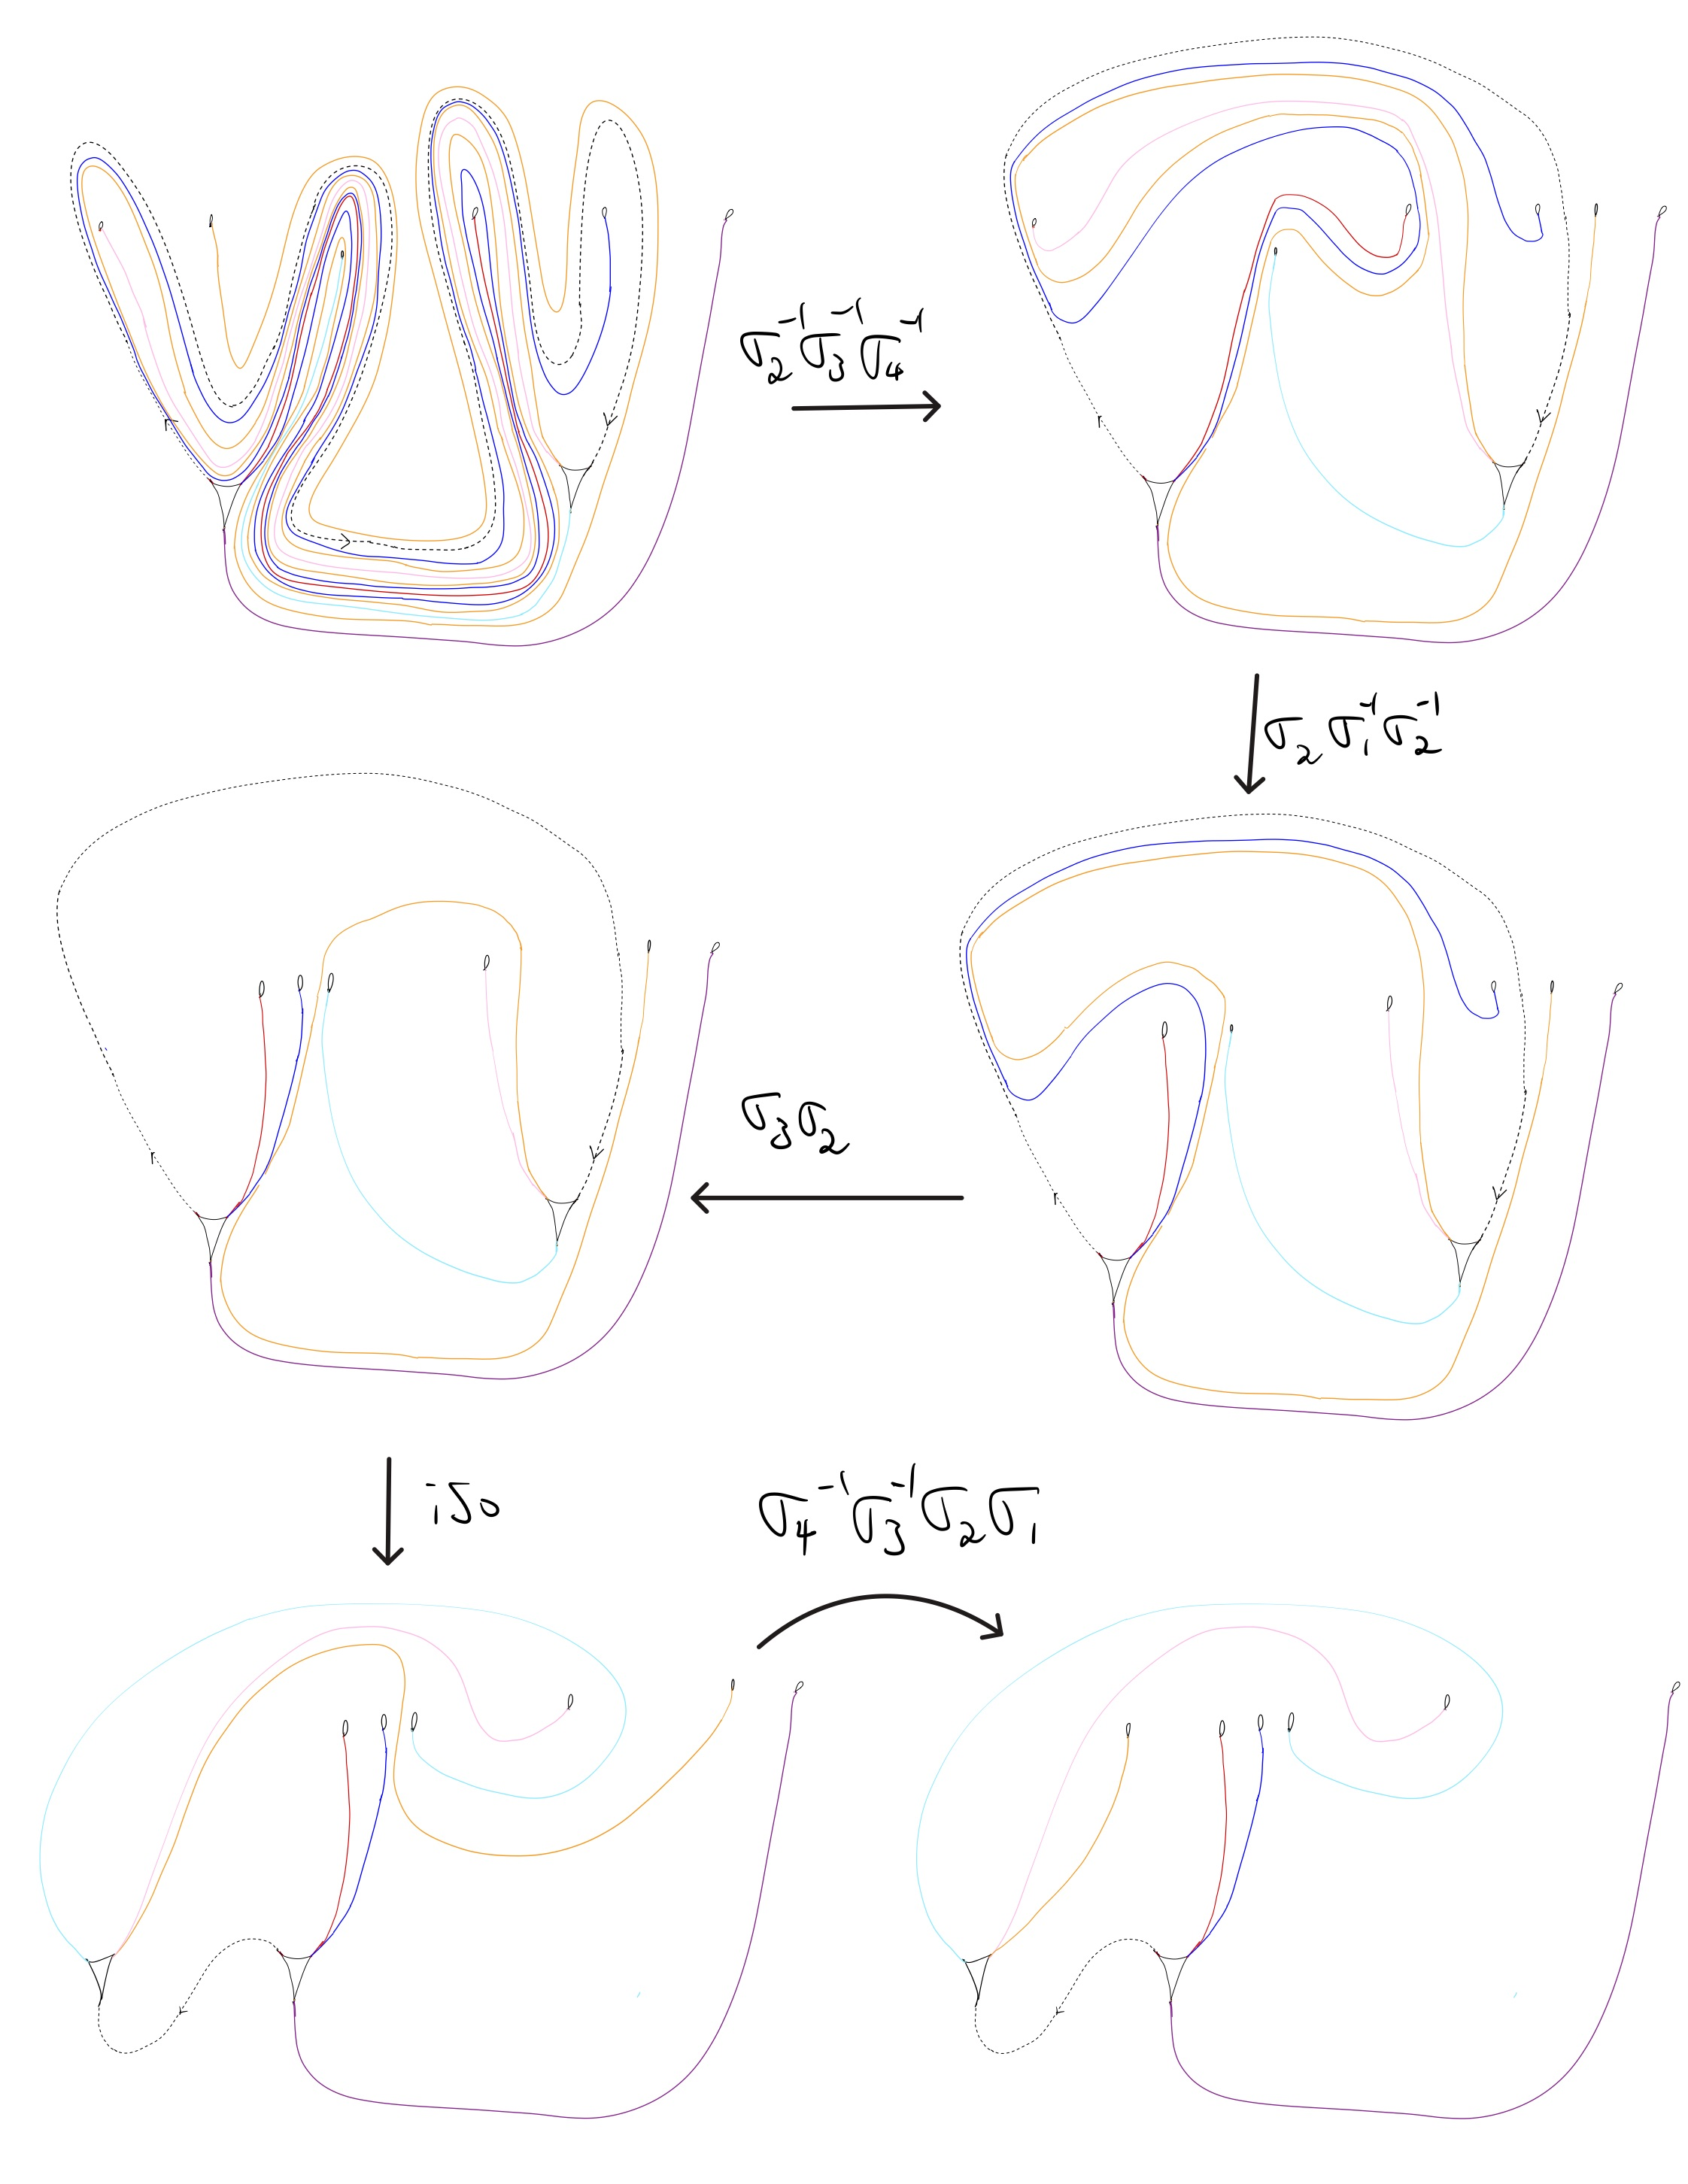
\includegraphics[width=\linewidth, height=0.45\textheight, keepaspectratio]{figures_braid/figures_track_0/Track 0 Braid 3 Mooncalf-2.jpg}\\
    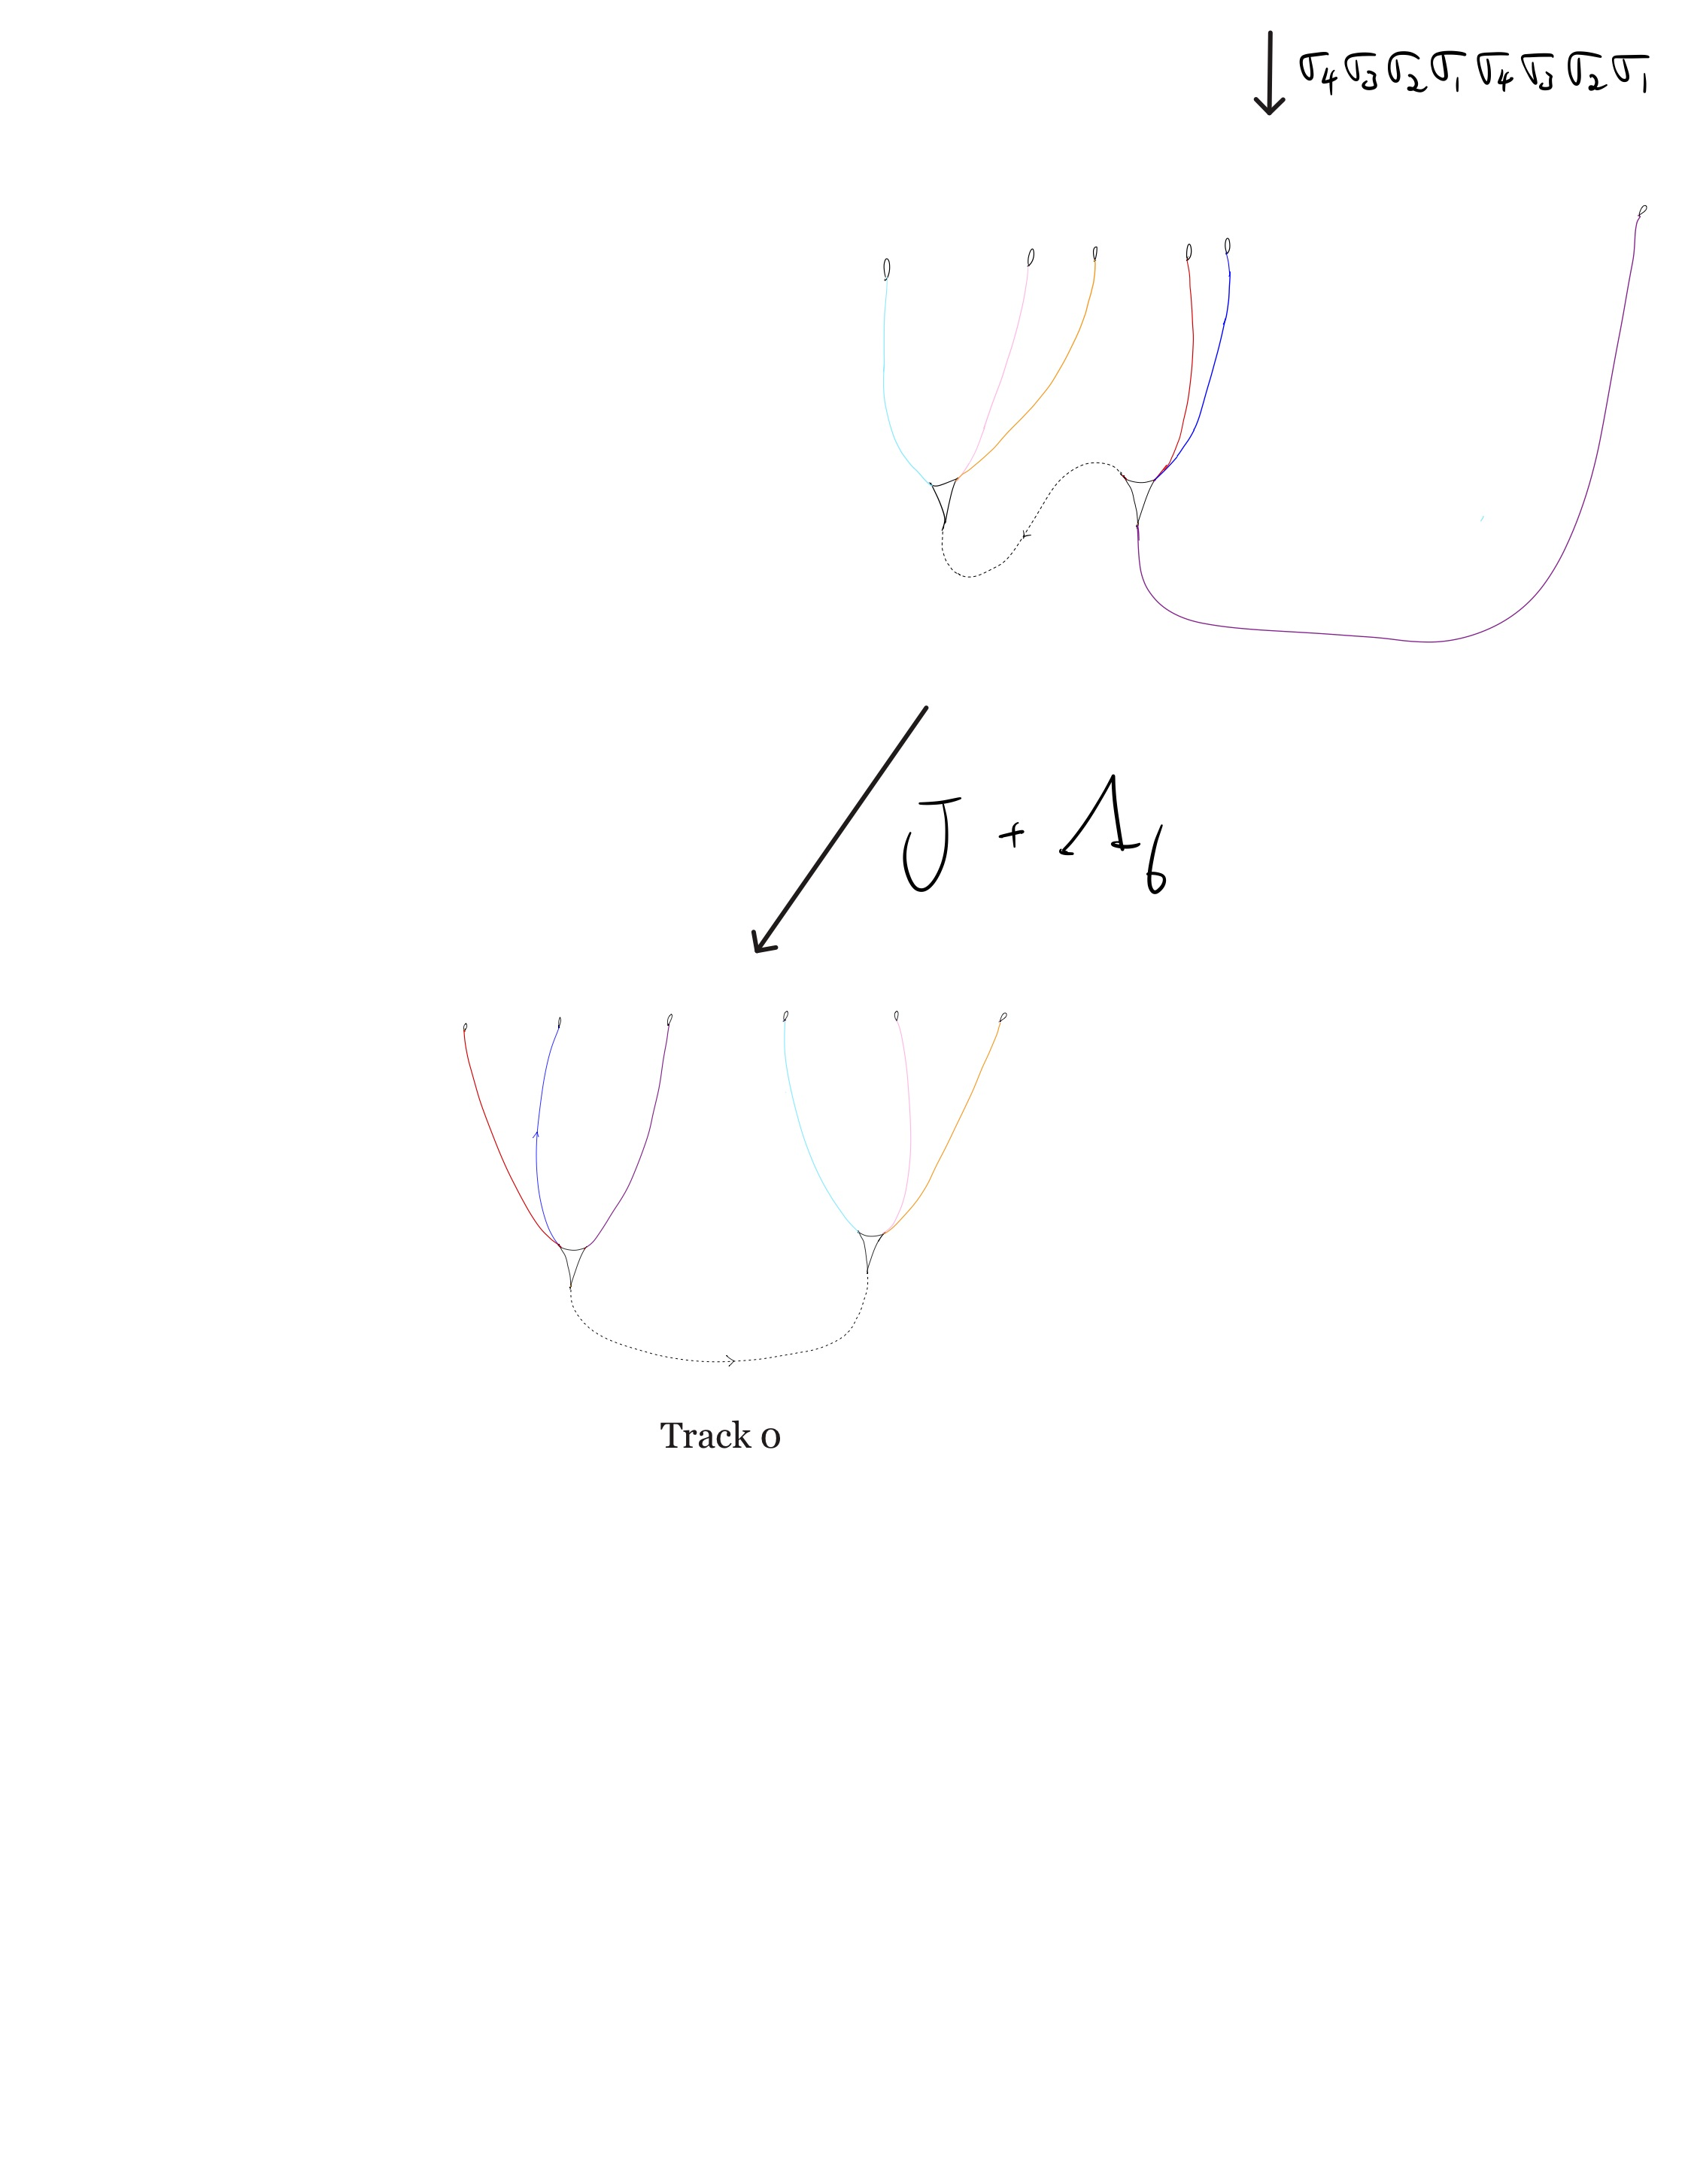
\includegraphics[width=\linewidth, height=0.45\textheight, keepaspectratio]{figures_braid/figures_track_0/Track 0 Braid 3 Mooncalf-3.jpg}
    \caption{This sequence shows the inverse of the braid $b_3^0$ carries Train Track Candidate Family 3.}
    \label{fig:track0_braid_b0_3}
\end{figure*}

\clearpage

\section{Candidate Family 4 (Faffel)}\label{sec:track0_faffel}
Train Track Map Candidate Family 4 of Track 0 is shown in Figure \ref{fig:track0_braid_b0_4_map}. See \ref{Faffel} for details.

\begin{figure*}[ht]
    \centering
    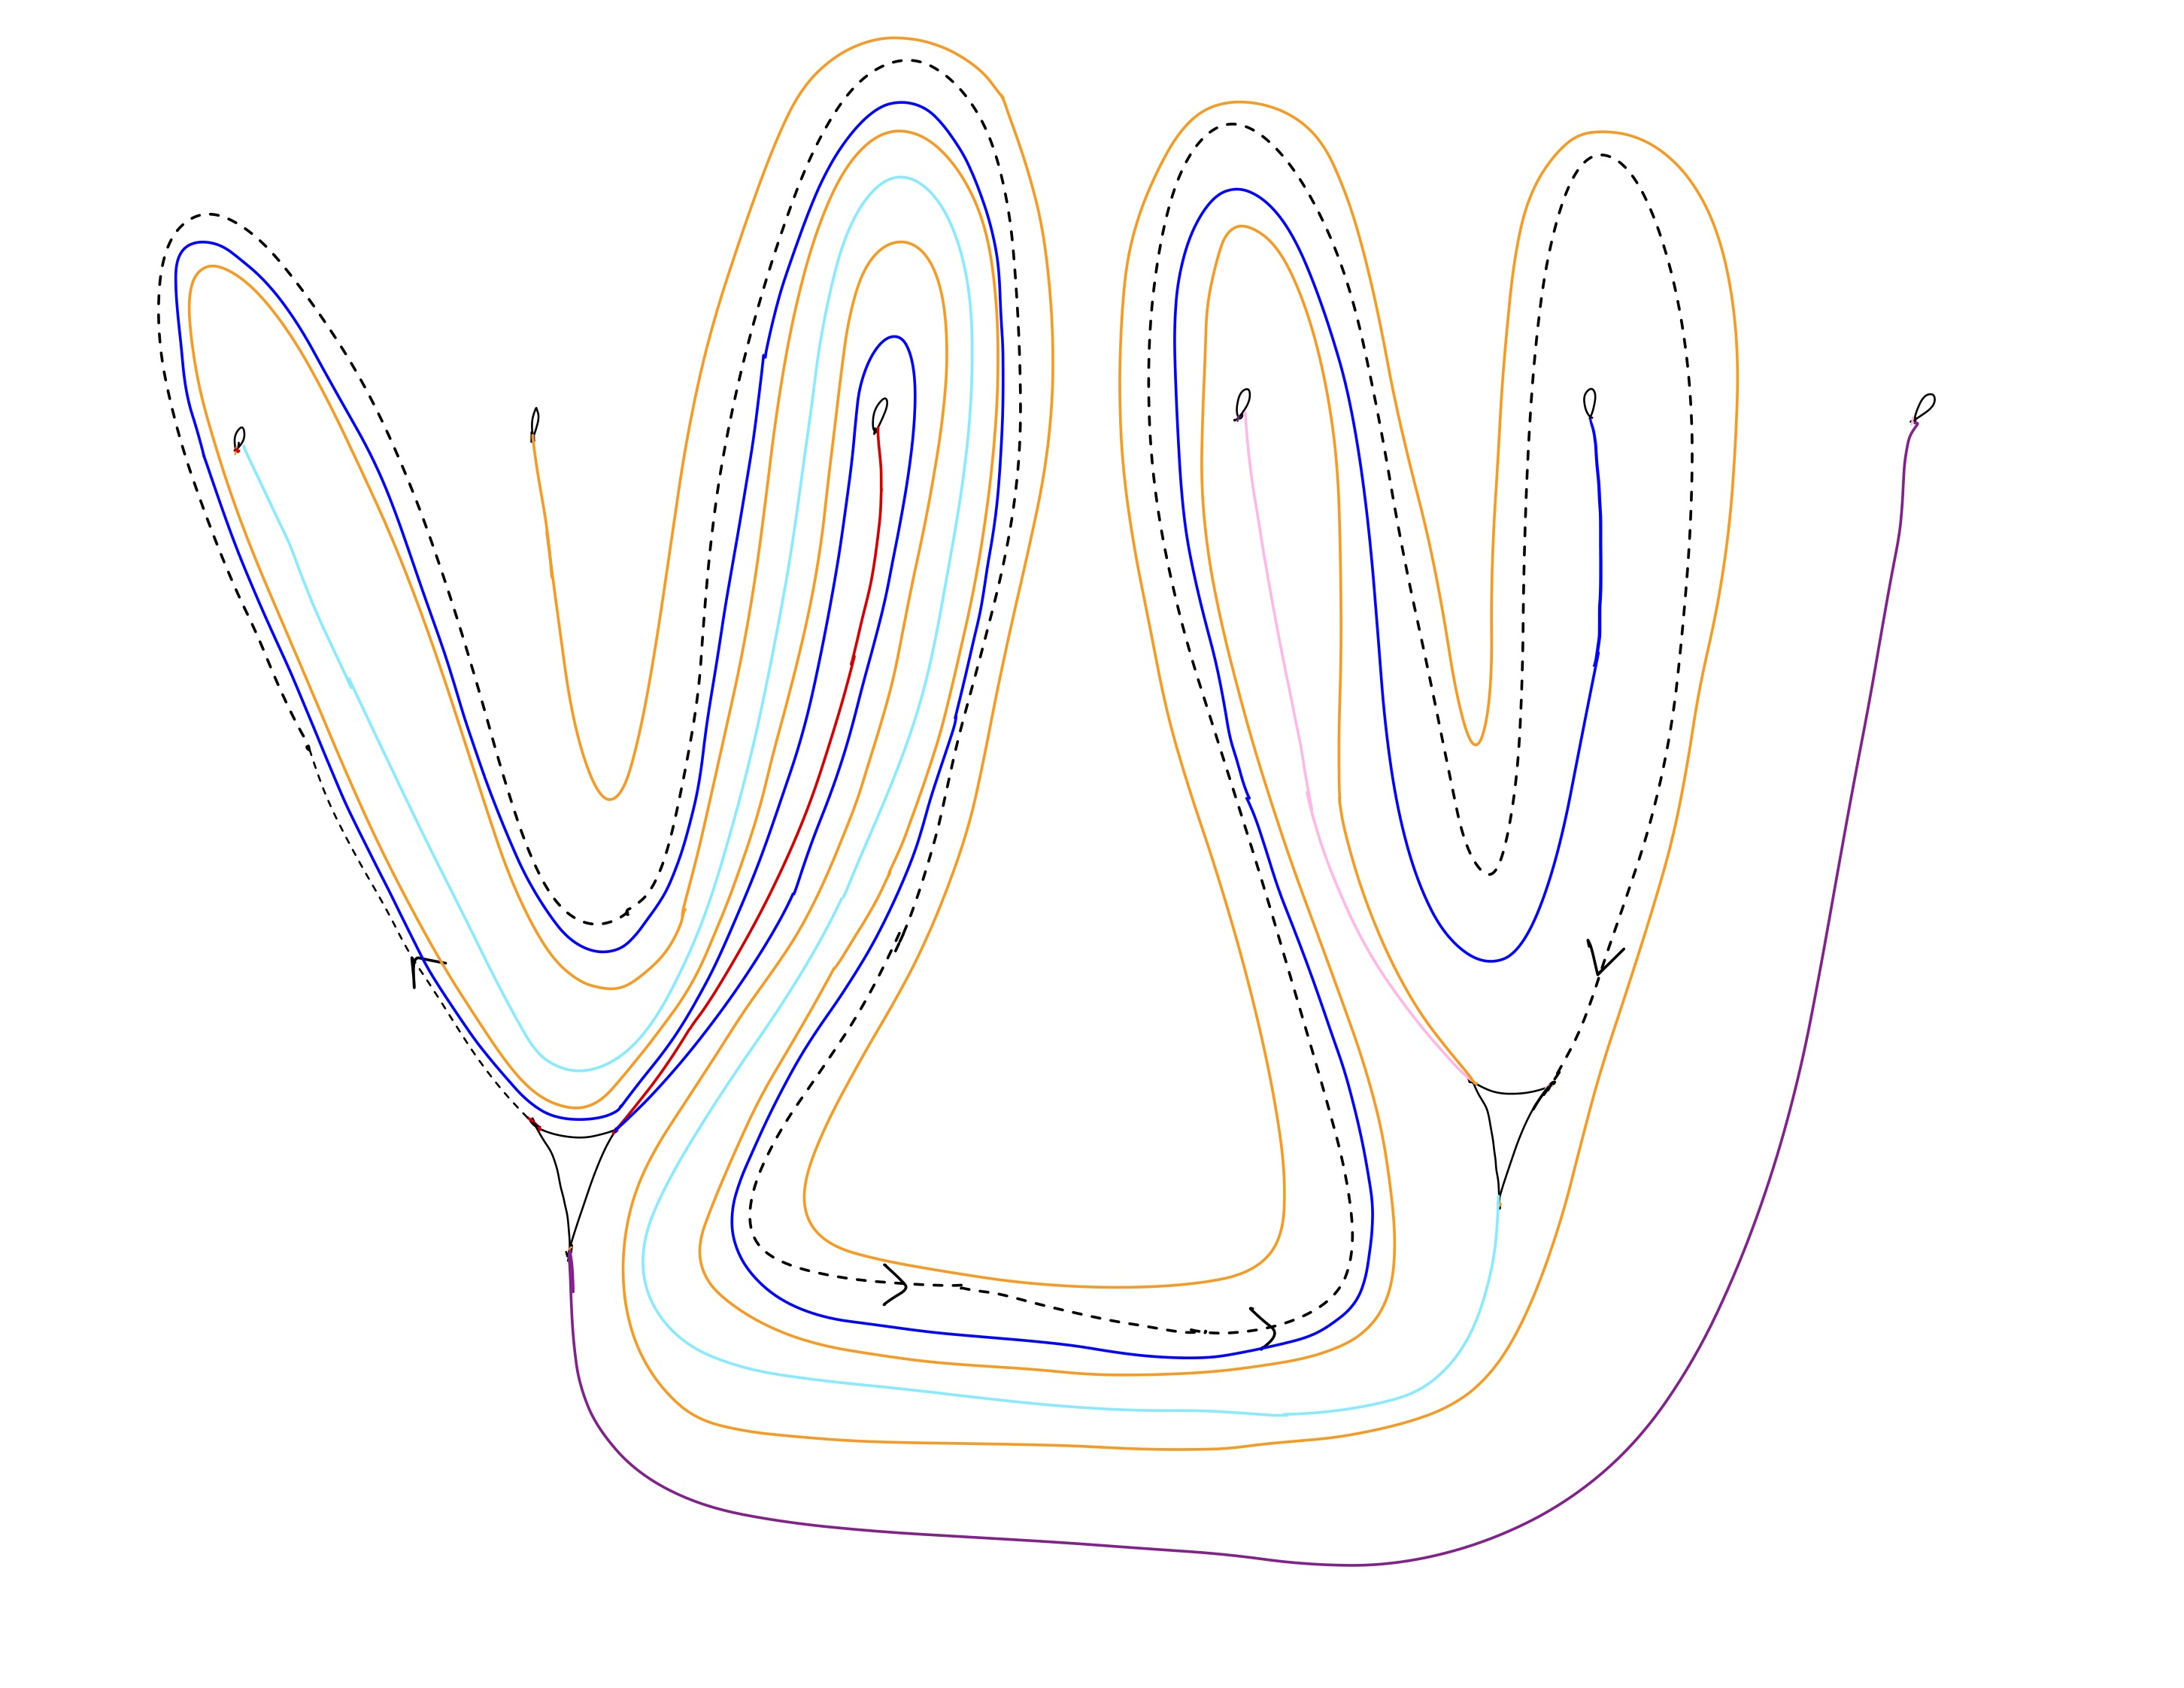
\includegraphics[width=\linewidth, height=0.45\textheight, keepaspectratio]{figures_braid/figures_track_0/Track 0 Braid 4 Faffel-1.jpg}
    \caption{Train Track Map Candidate Family 4 of Track 0.}
    \label{fig:track0_braid_b0_4_map}
\end{figure*}

The inverse of the following braid carries this family of train track maps:
\[
b_4^0 = \sigma_{2}^{-1} \sigma_{3}^{-1} \sigma_{4}^{-1} \sigma_{1}^{-1} \sigma_{3} \sigma_{2} \sigma_{4}^{-1} \sigma_{3}^{-1} \sigma_{2} \sigma_{1} \sigma_{4} \sigma_{4} \sigma_{3} \sigma_{2} \sigma_{1} \sigma_{4} \sigma_{3} \sigma_{2} \cdot J \cdot \Lambda_6
\]

This is shown in Figure \ref{fig:track0_braid_b0_4}.

\begin{figure*}[p]
    \centering
    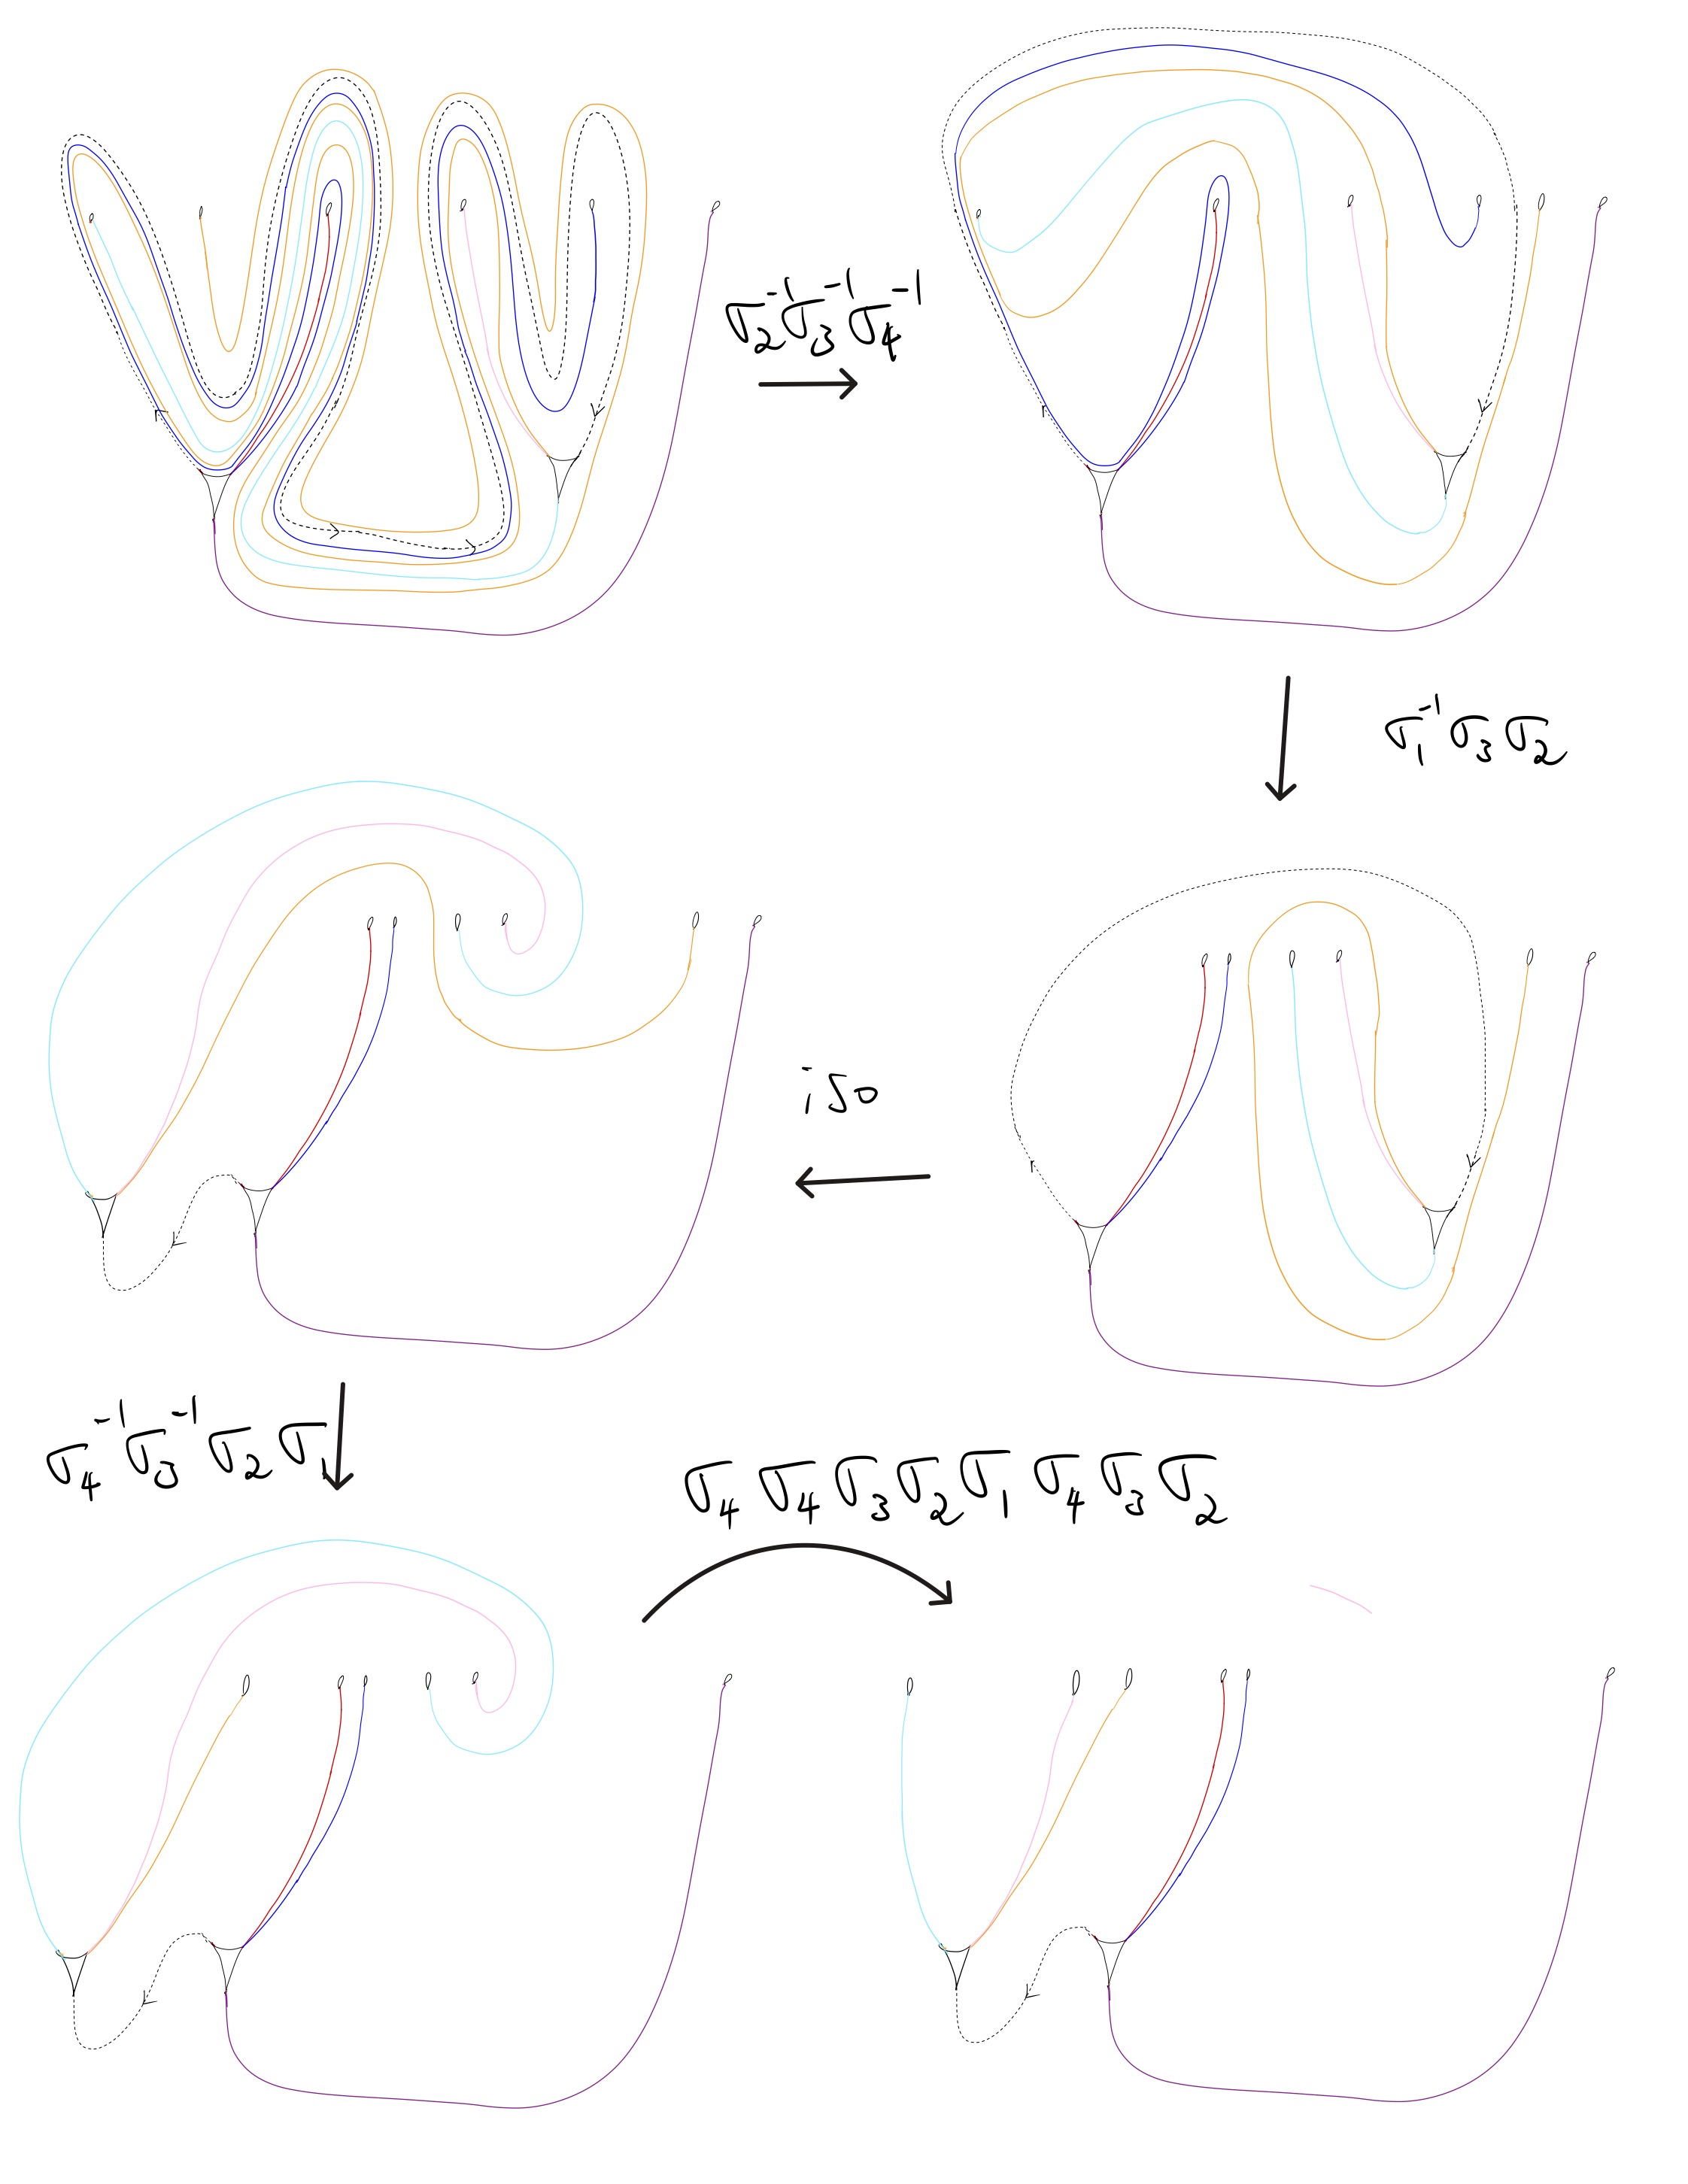
\includegraphics[width=\linewidth, height=0.45\textheight, keepaspectratio]{figures_braid/figures_track_0/Track 0 Braid 4 Faffel-2.jpg}\\
    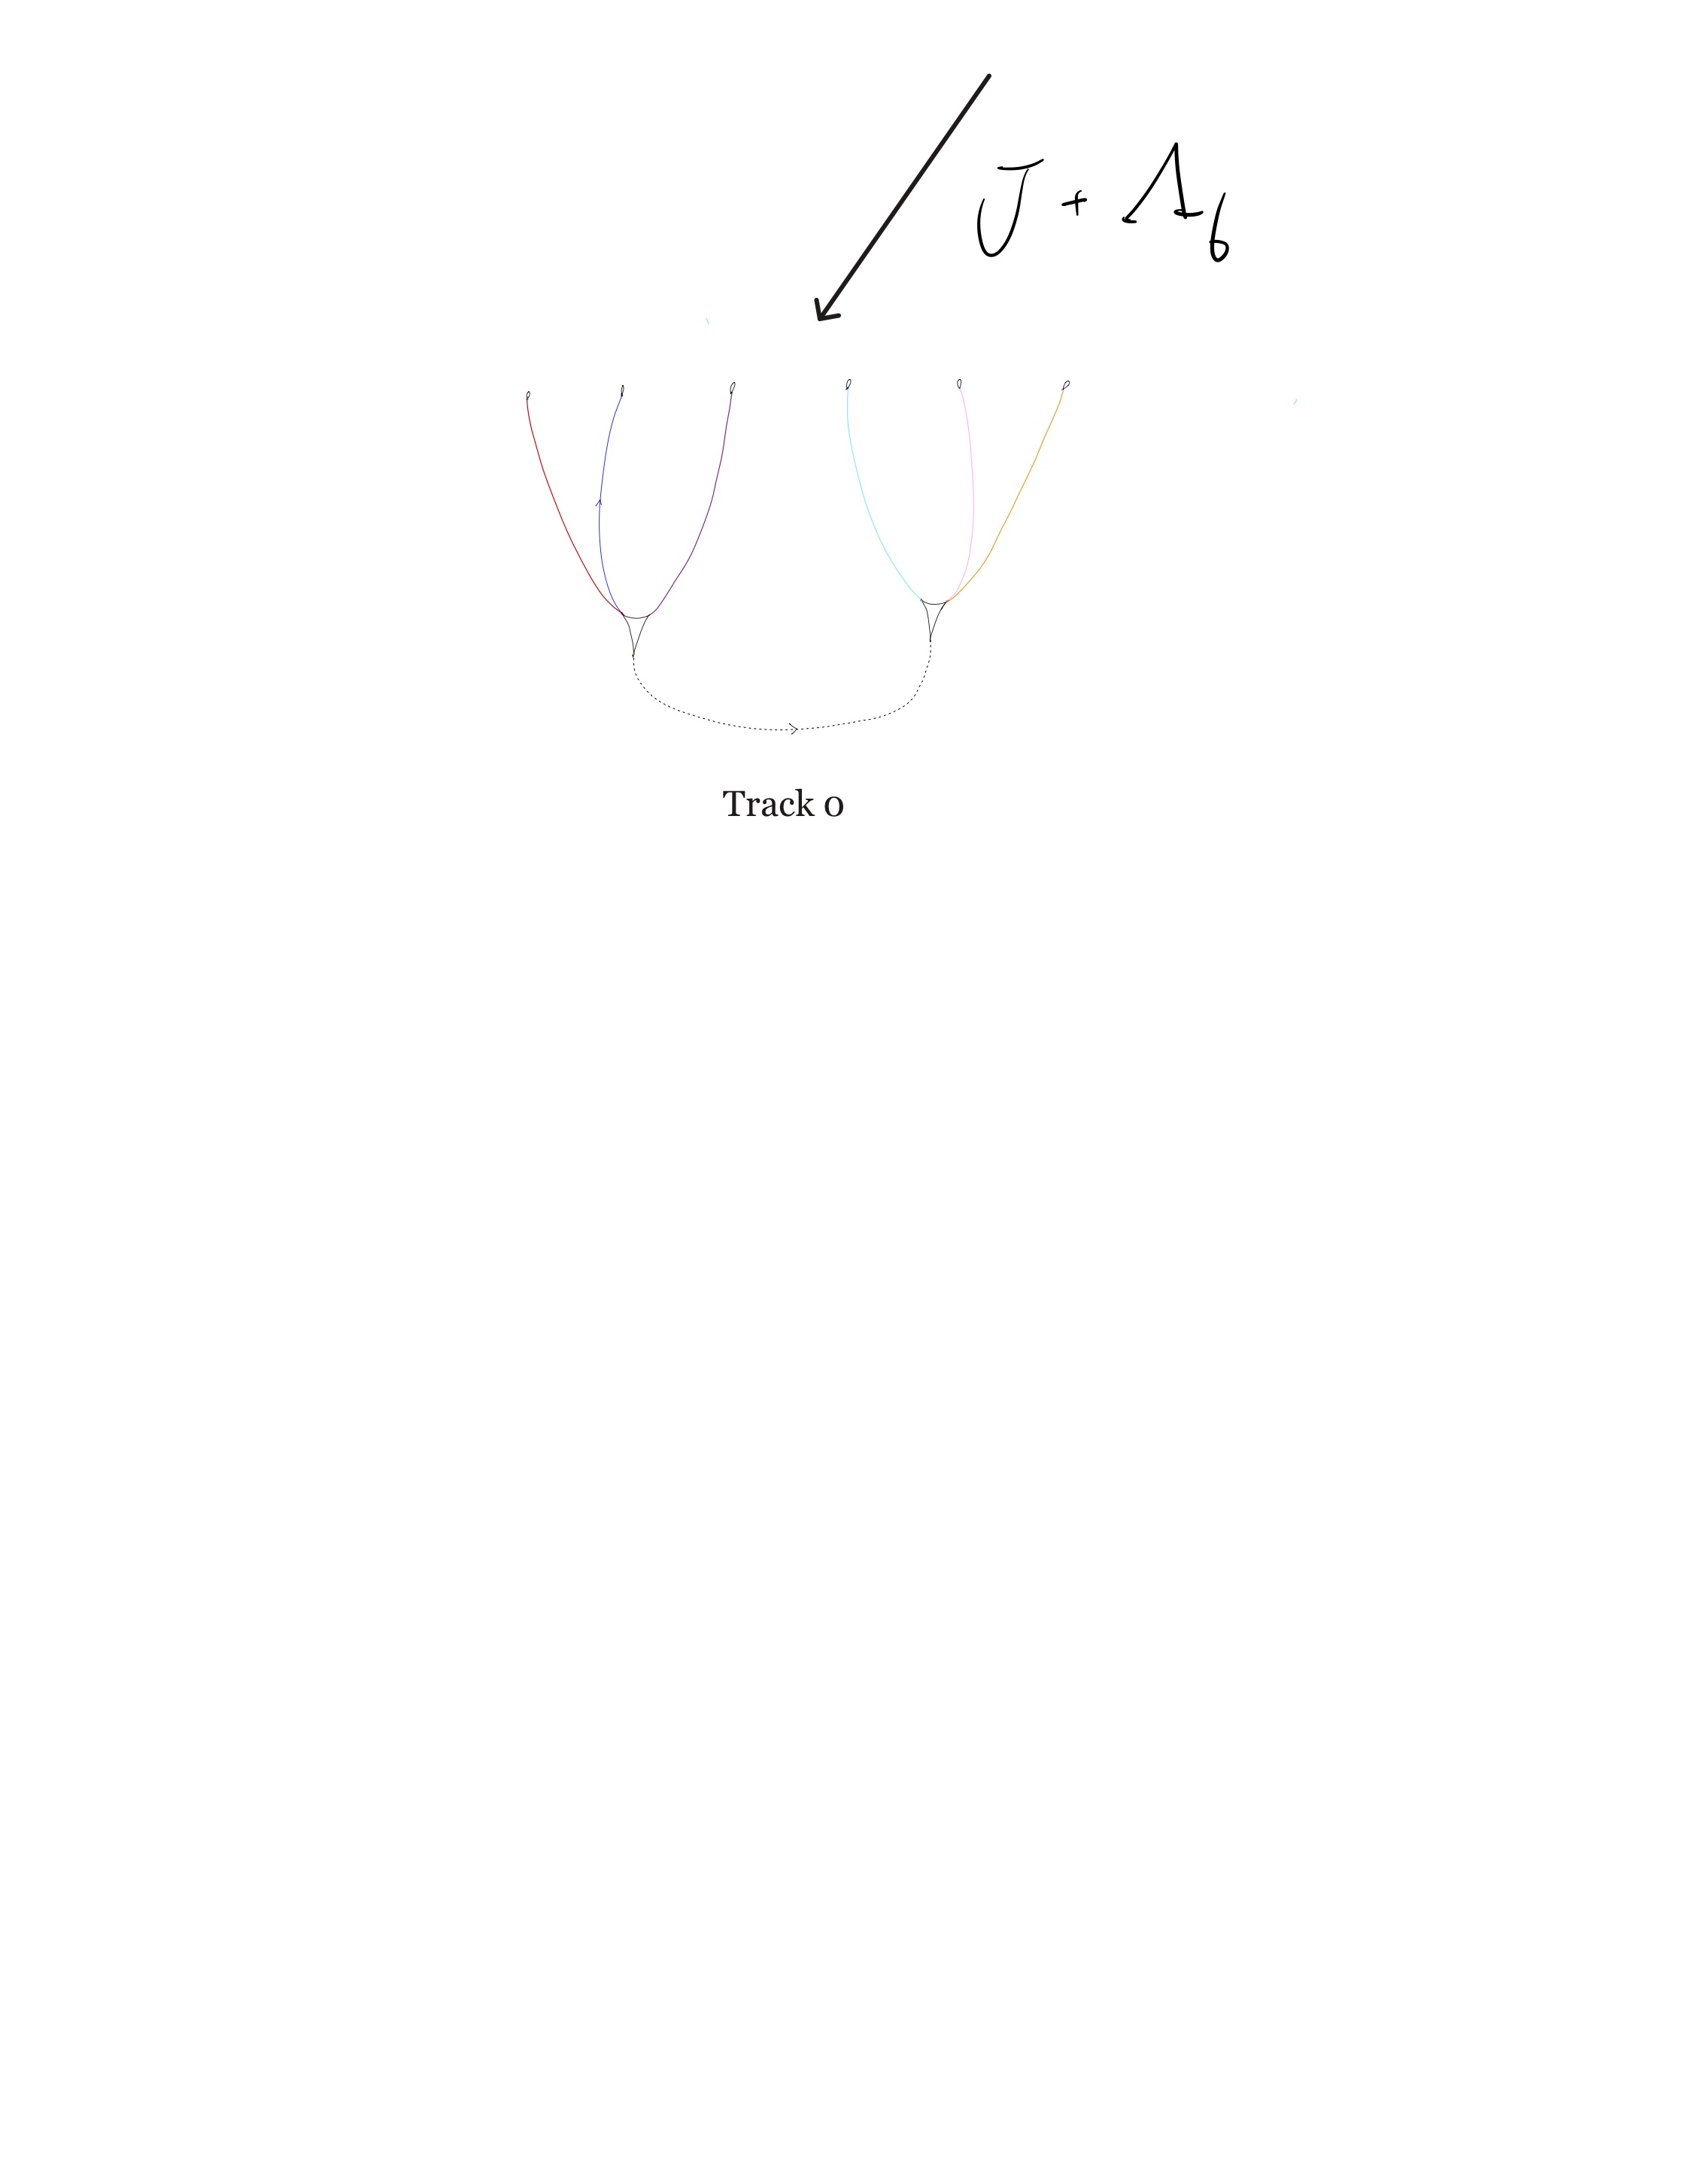
\includegraphics[width=\linewidth, height=0.45\textheight, keepaspectratio]{figures_braid/figures_track_0/Track 0 Braid 4 Faffel-3.jpg}
    \caption{This sequence shows the inverse of the braid $b_4^0$ carries Train Track Candidate Family 4.}
    \label{fig:track0_braid_b0_4}
\end{figure*}

\clearpage

\section{Candidate Family 5 (Balance)}\label{sec:track0_balance}
Train Track Map Candidate Family 5 of Track 0 is shown in Figure \ref{fig:track0_braid_b0_5_map}. See \ref{Balance} for details.

\begin{figure*}[ht]
    \centering
    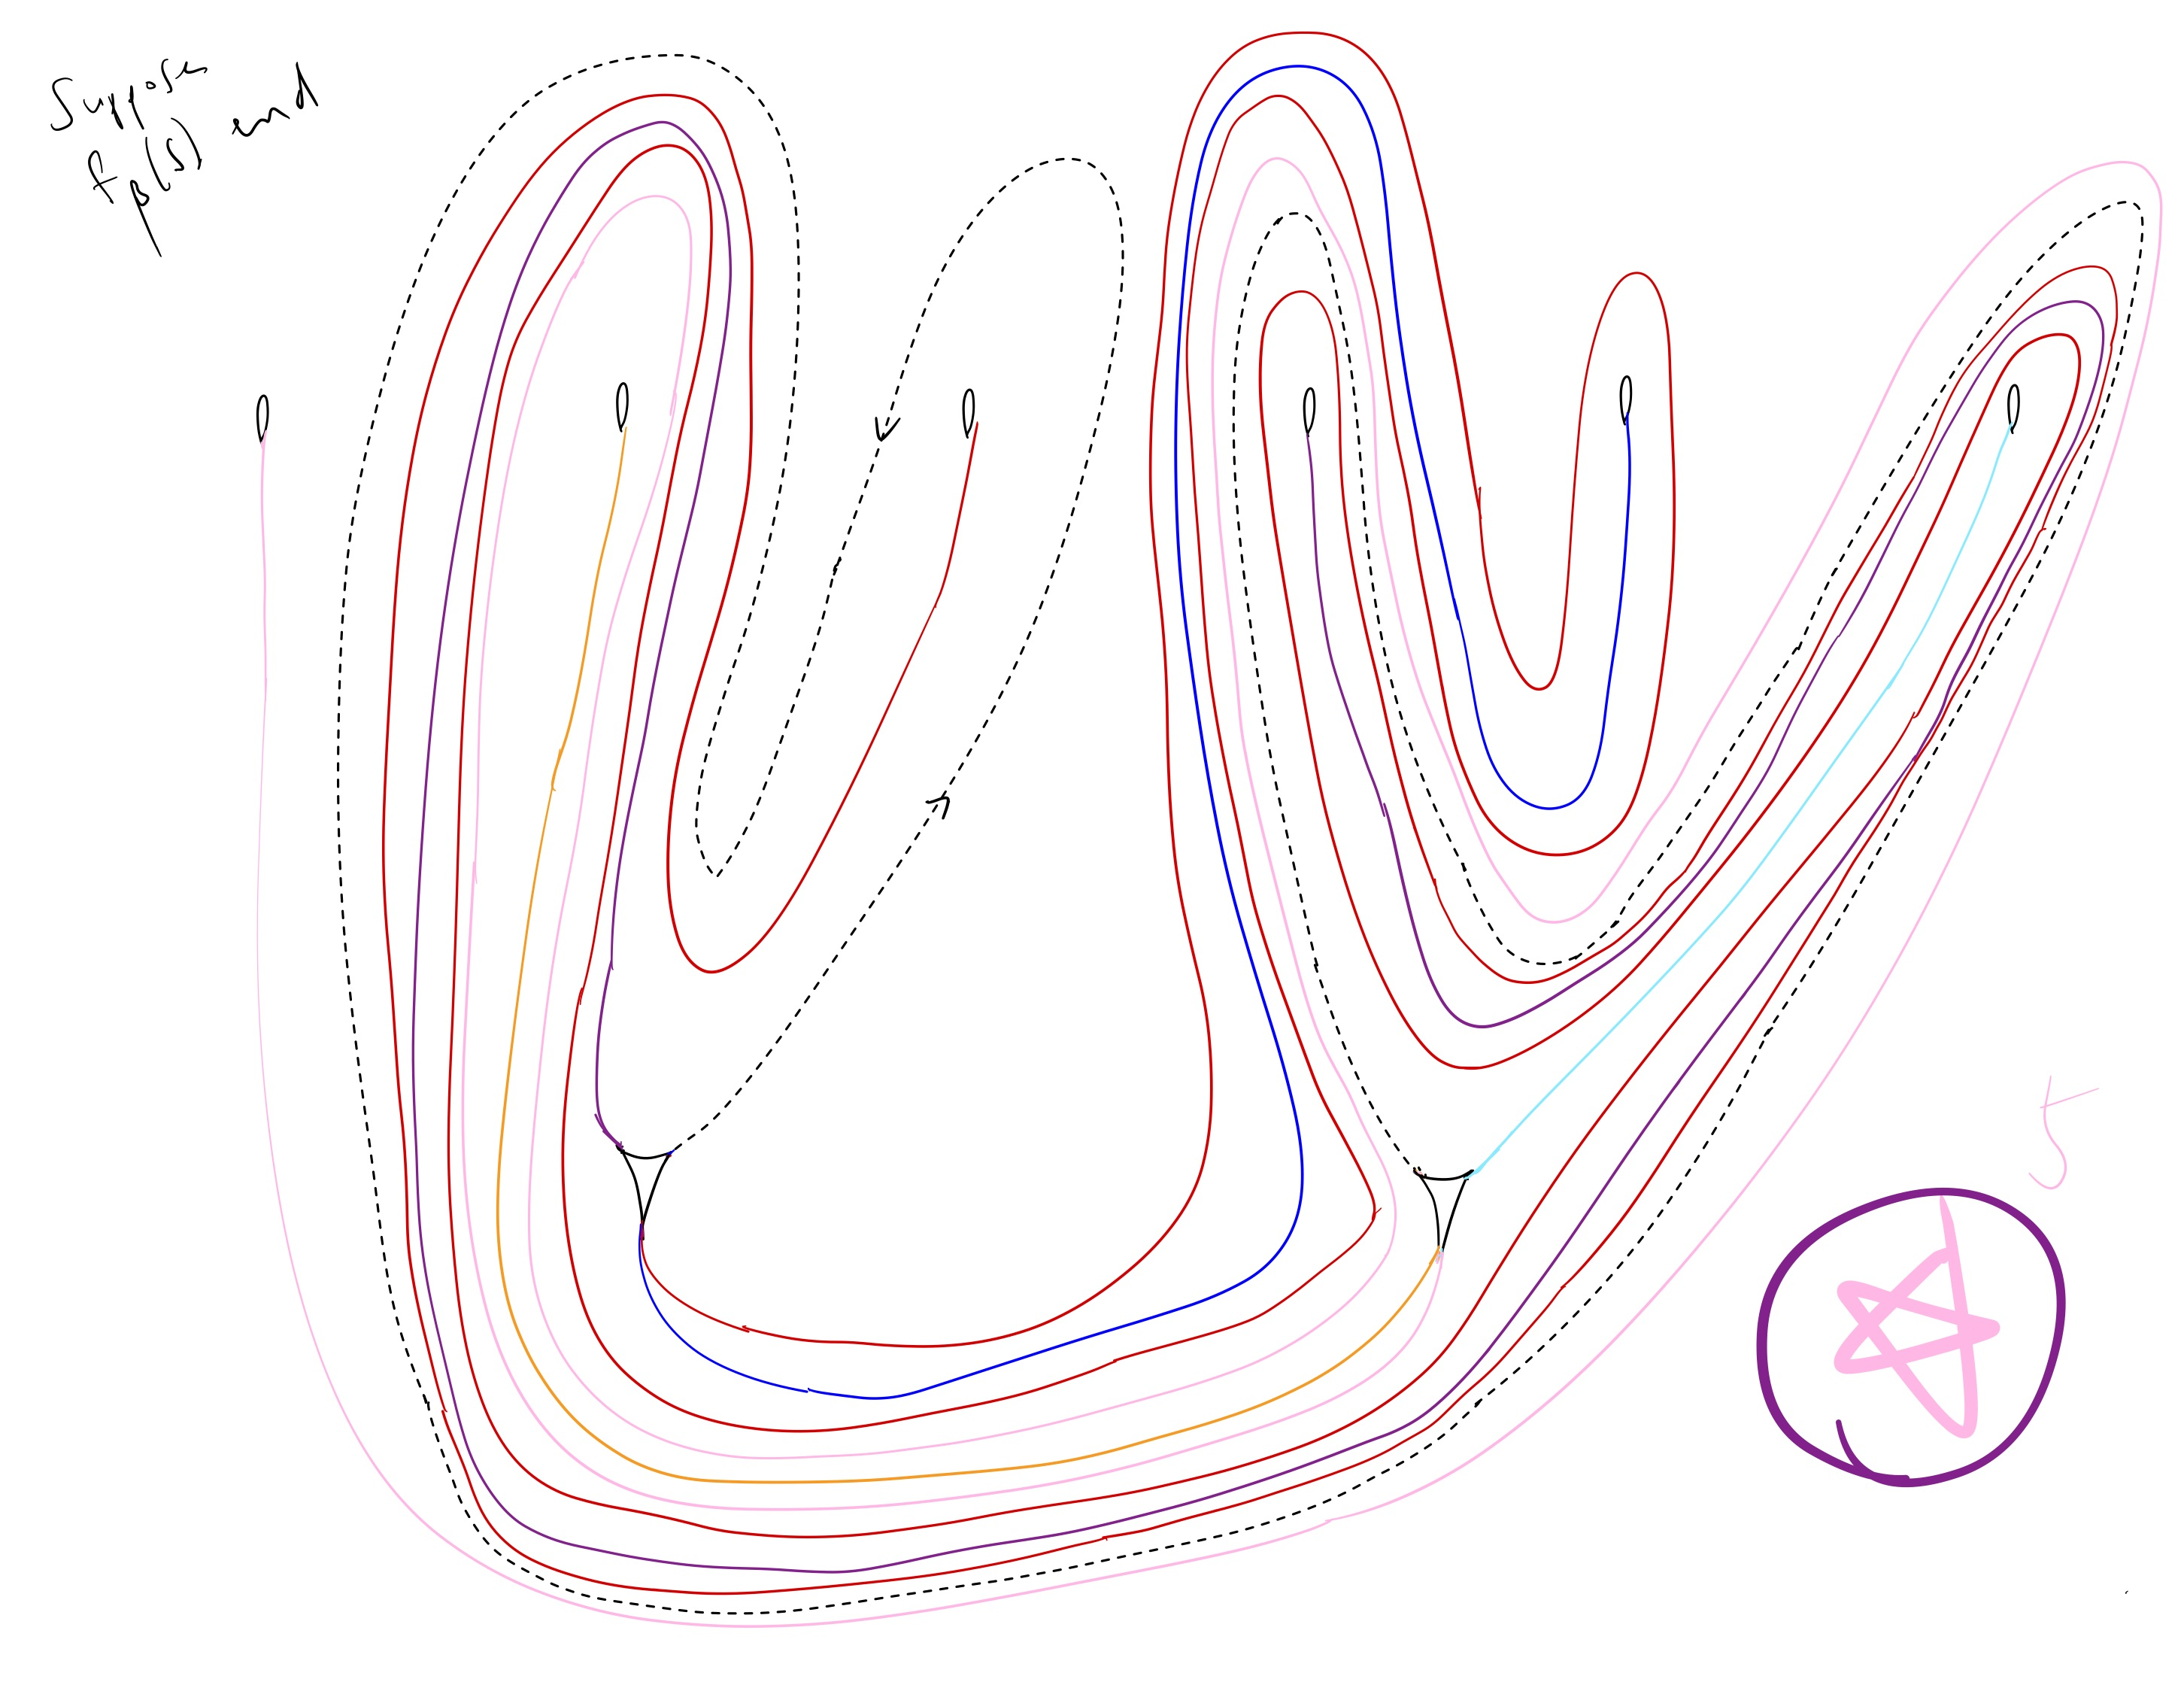
\includegraphics[width=\linewidth, height=0.45\textheight, keepaspectratio]{figures_braid/figures_track_0/Track 0 Braid 5 Balance-1.jpg}
    \caption{Train Track Map Candidate Family 5 of Track 0.}
    \label{fig:track0_braid_b0_5_map}
\end{figure*}

The inverse of the following braid carries this family of train track maps:
\[
b_5^0 = \sigma_{4} \sigma_{2} \sigma_{5}^{-1} \sigma_{3} \sigma_{2} \sigma_{1} \sigma_{4}^{-1} \sigma_{5}^{-1} \sigma_{4}^{-1} \sigma_{3} \sigma_{2} \sigma_{3} \sigma_{2} \sigma_{1} \sigma_{4} \sigma_{5} \sigma_{5}
\]

This is shown in Figure \ref{fig:track0_braid_b0_5}.

\begin{figure*}[p]
    \centering
    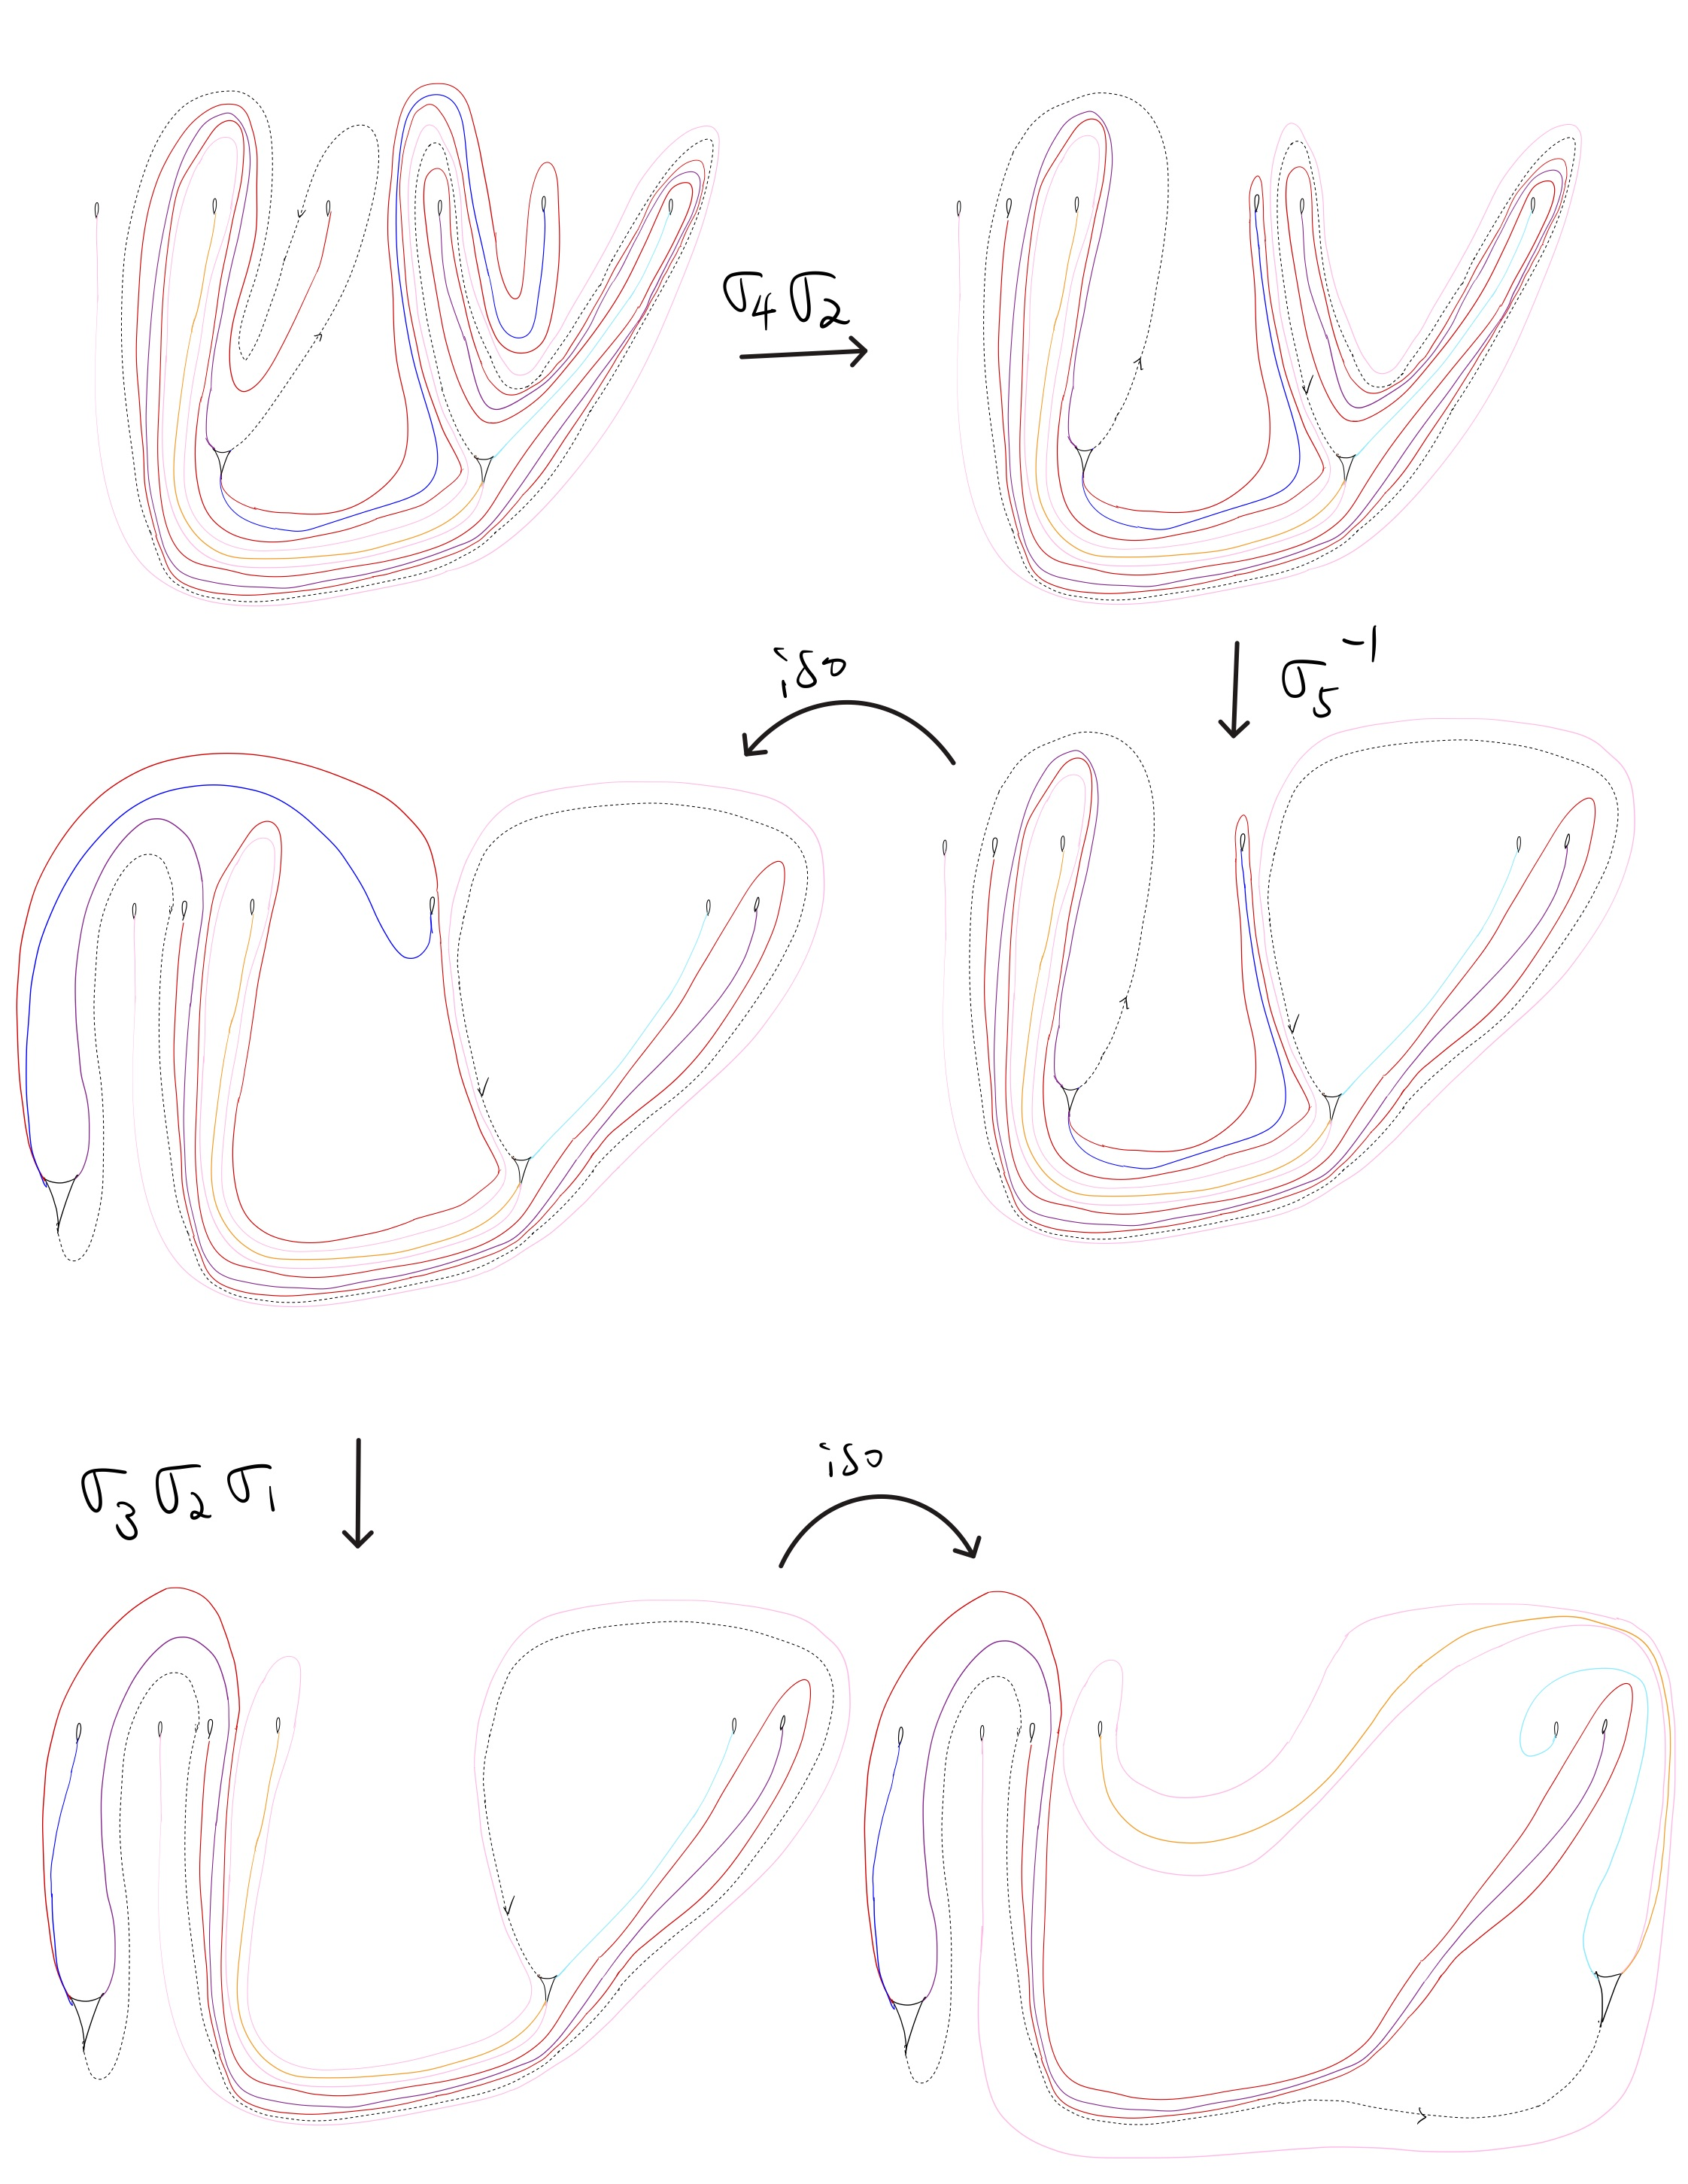
\includegraphics[width=\linewidth, height=0.45\textheight, keepaspectratio]{figures_braid/figures_track_0/Track 0 Braid 5 Balance-2.jpg}\\
    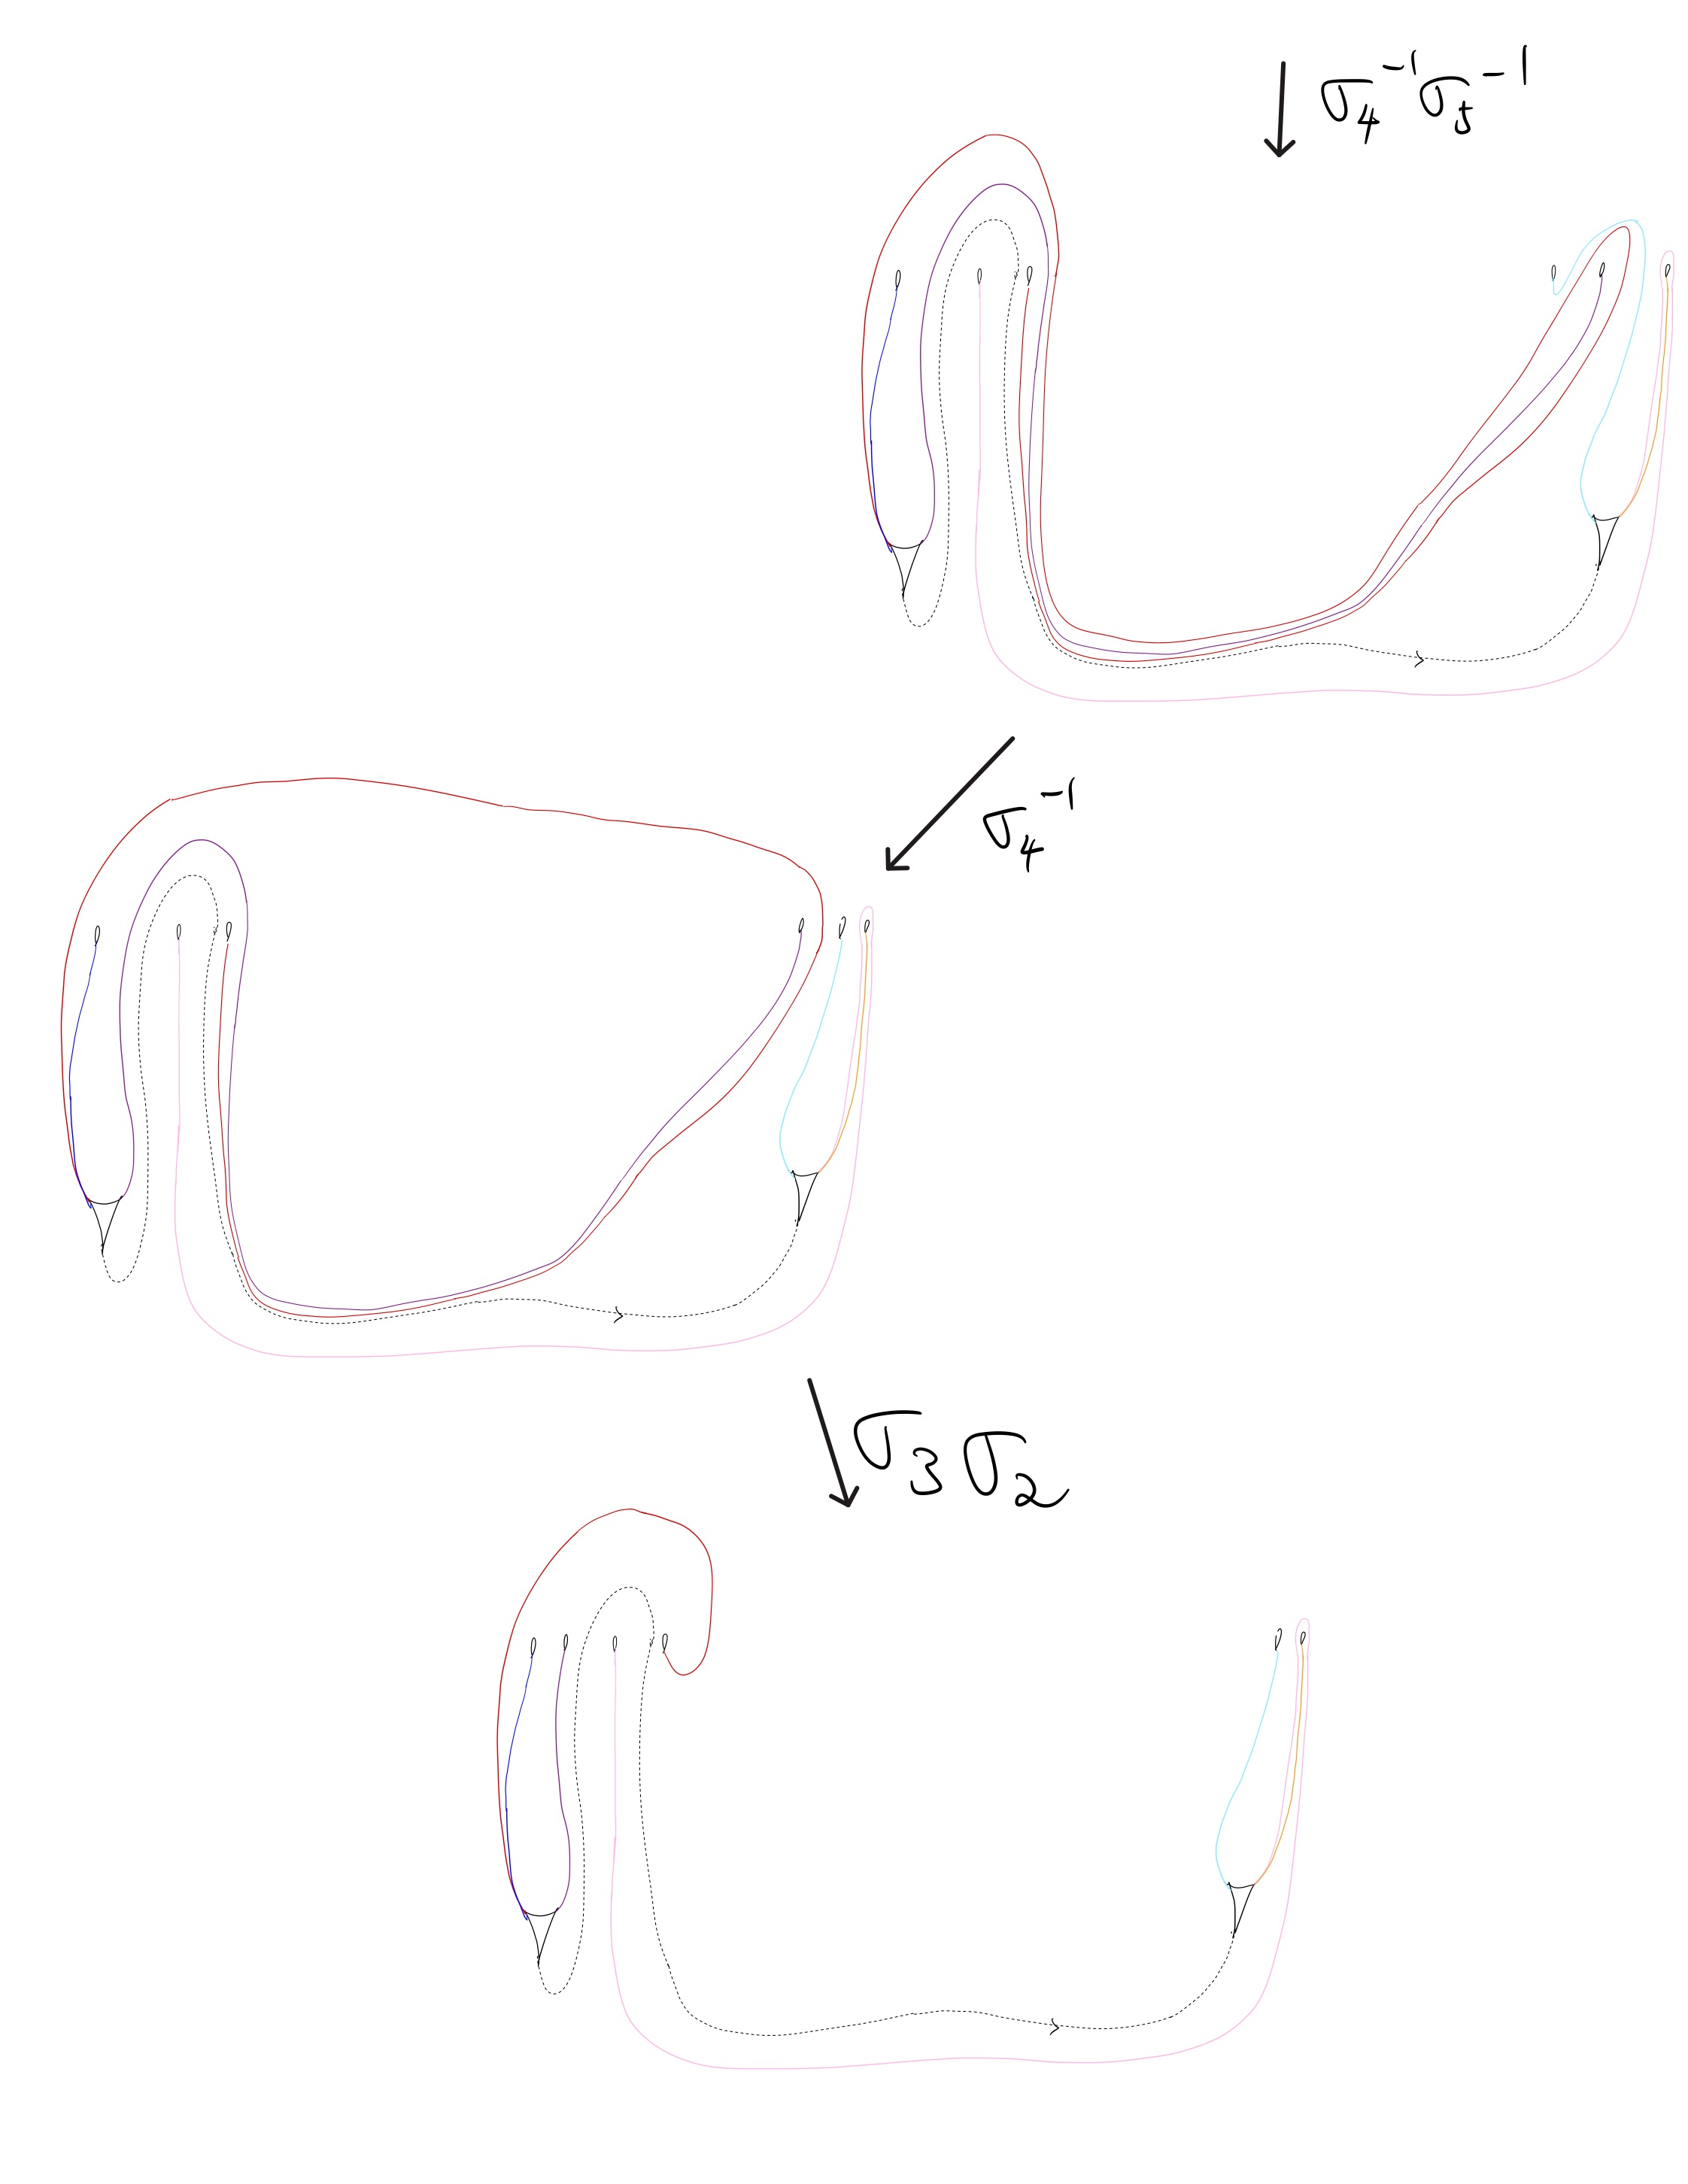
\includegraphics[width=\linewidth, height=0.45\textheight, keepaspectratio]{figures_braid/figures_track_0/Track 0 Braid 5 Balance-3.jpg}
    \caption{This sequence shows the inverse of the braid $b_5^0$ carries Train Track Candidate 5.}
    \label{fig:track0_braid_b0_5}
\end{figure*}

\begin{figure*}[p]
    \ContinuedFloat
    \centering
    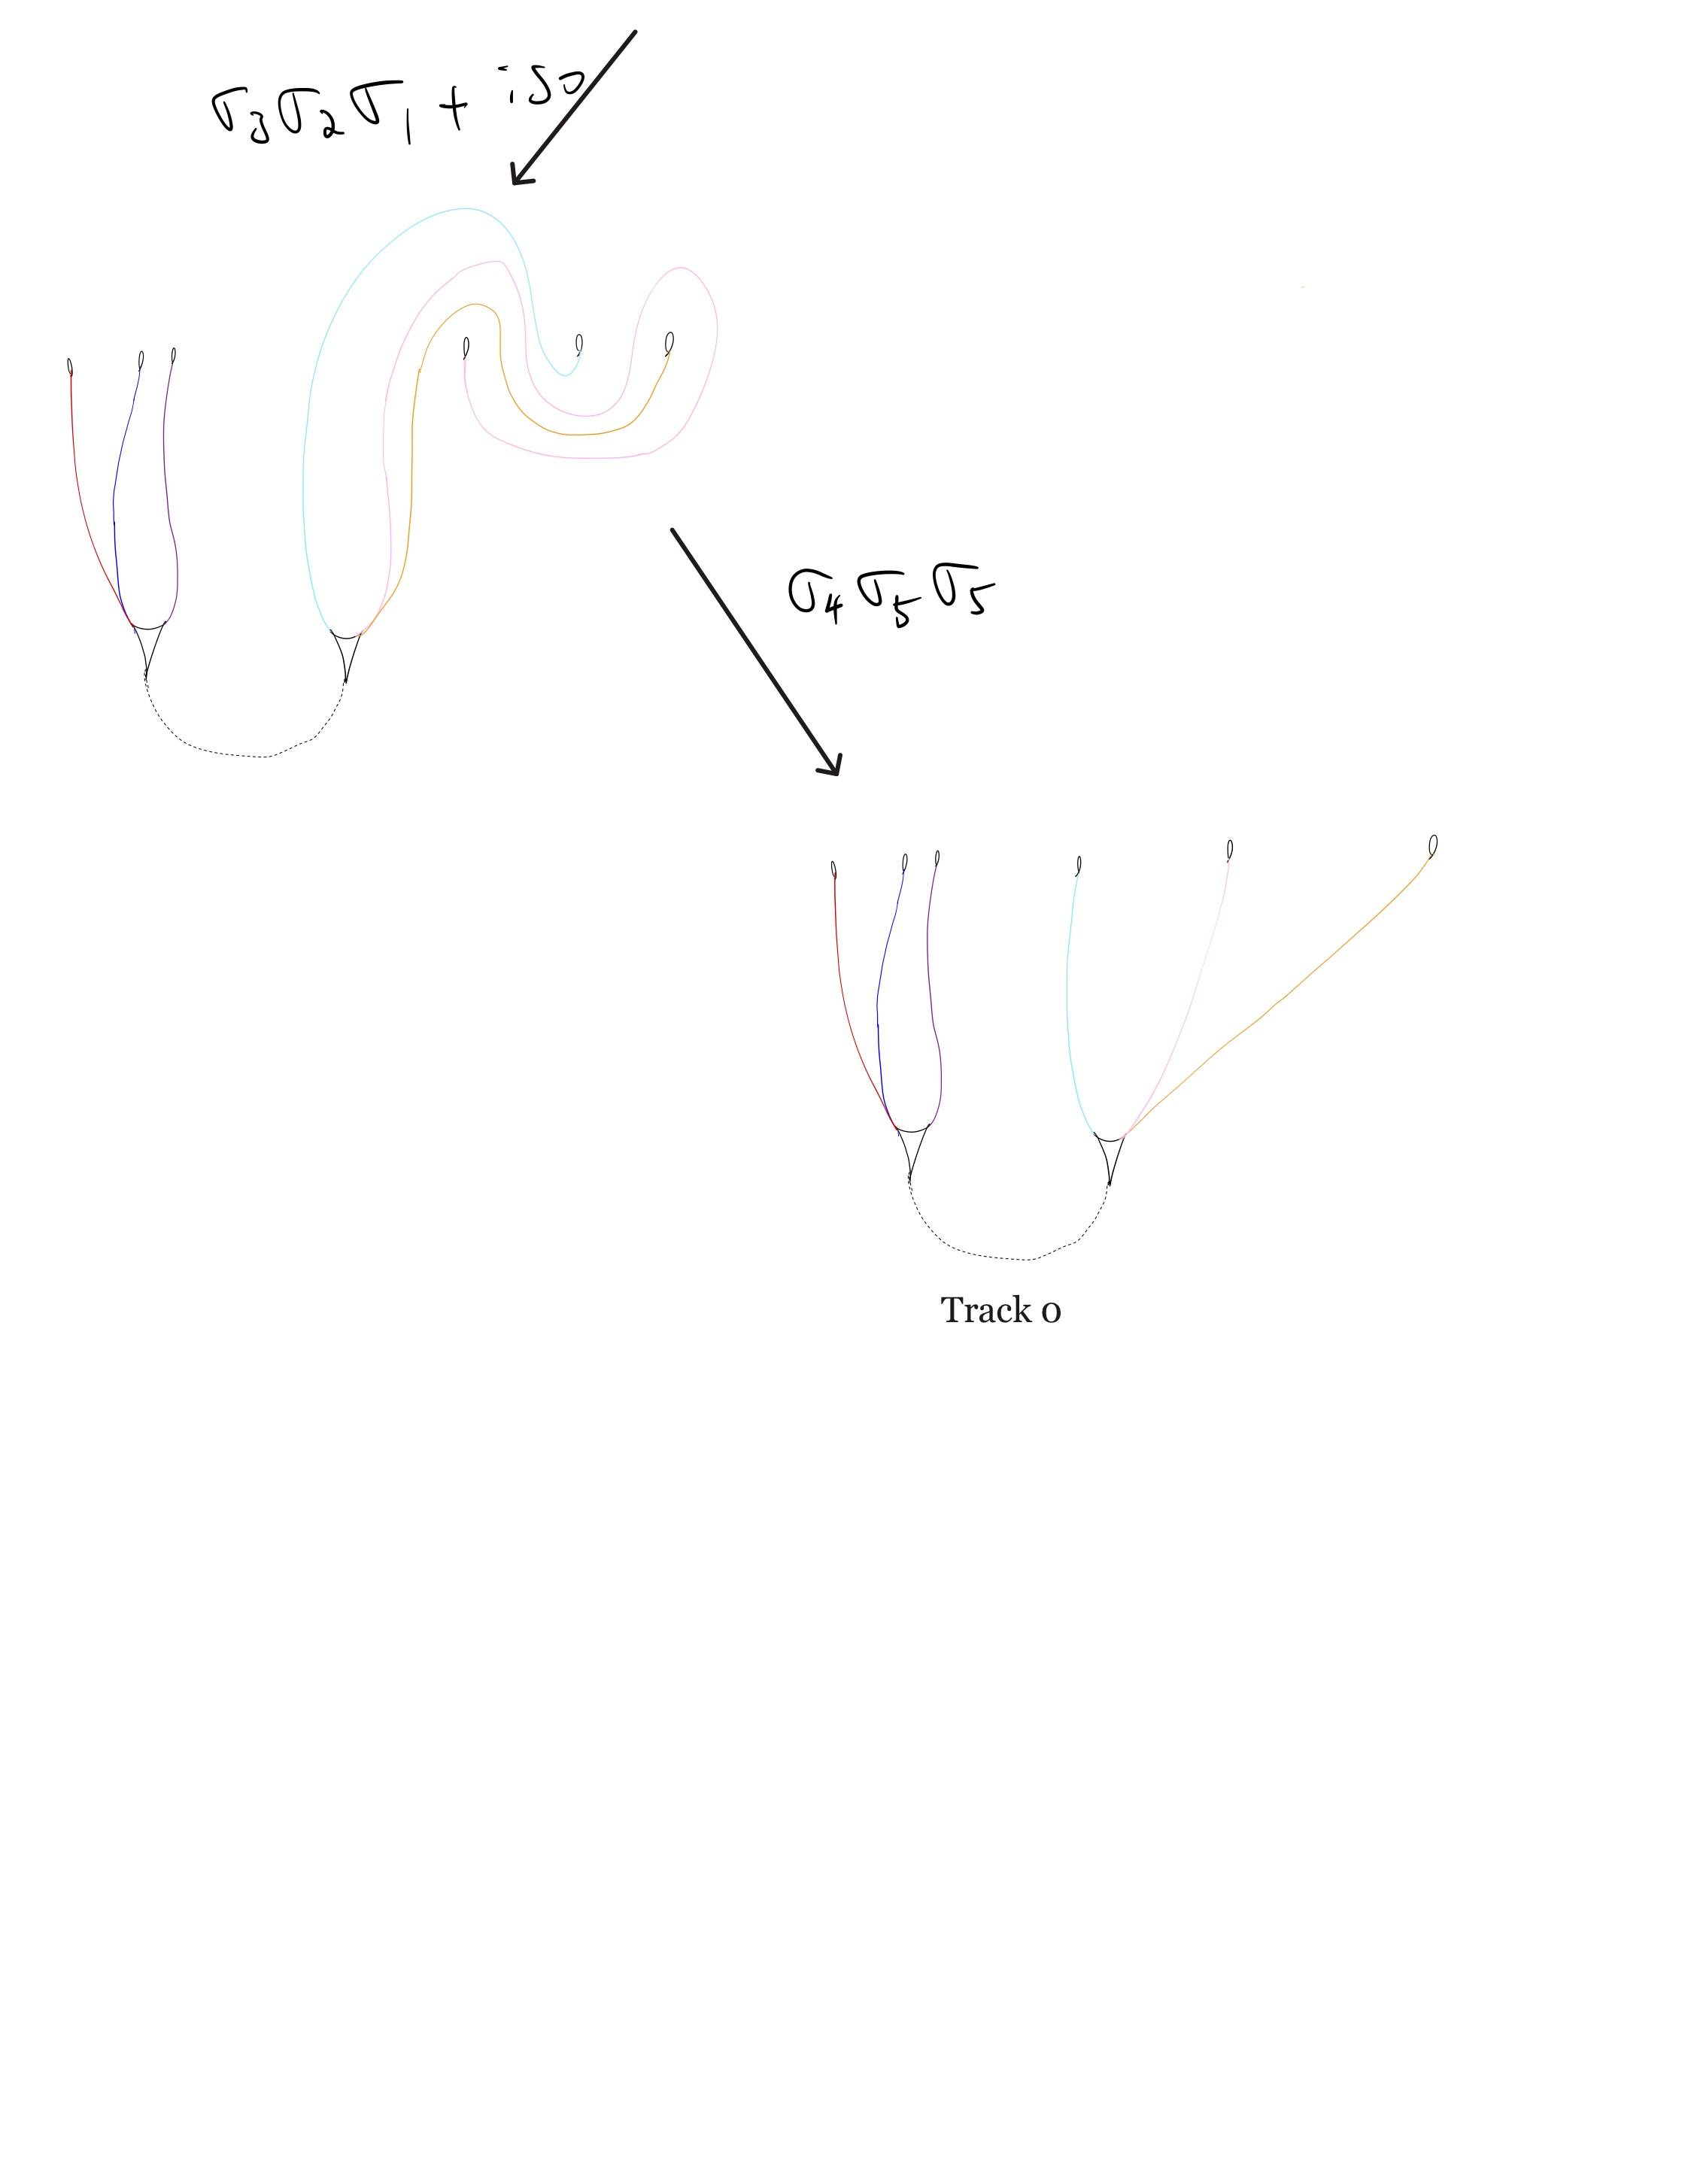
\includegraphics[width=\linewidth, height=0.45\textheight, keepaspectratio]{figures_braid/figures_track_0/Track 0 Braid 5 Balance-4.jpg}
    \caption[]{This sequence shows the inverse of the braid $b_5^0$ carries Train Track Candidate 5 (continued).}
\end{figure*}

\clearpage

\section{Candidate Family 6 (Fiasco)}\label{sec:track0_fiasco}
Train Track Map Candidate Family 6 of Track 0 is shown in Figure \ref{fig:track0_braid_b0_6_map}. See \ref{Fiasco} for details.

\begin{figure*}[ht]
    \centering
    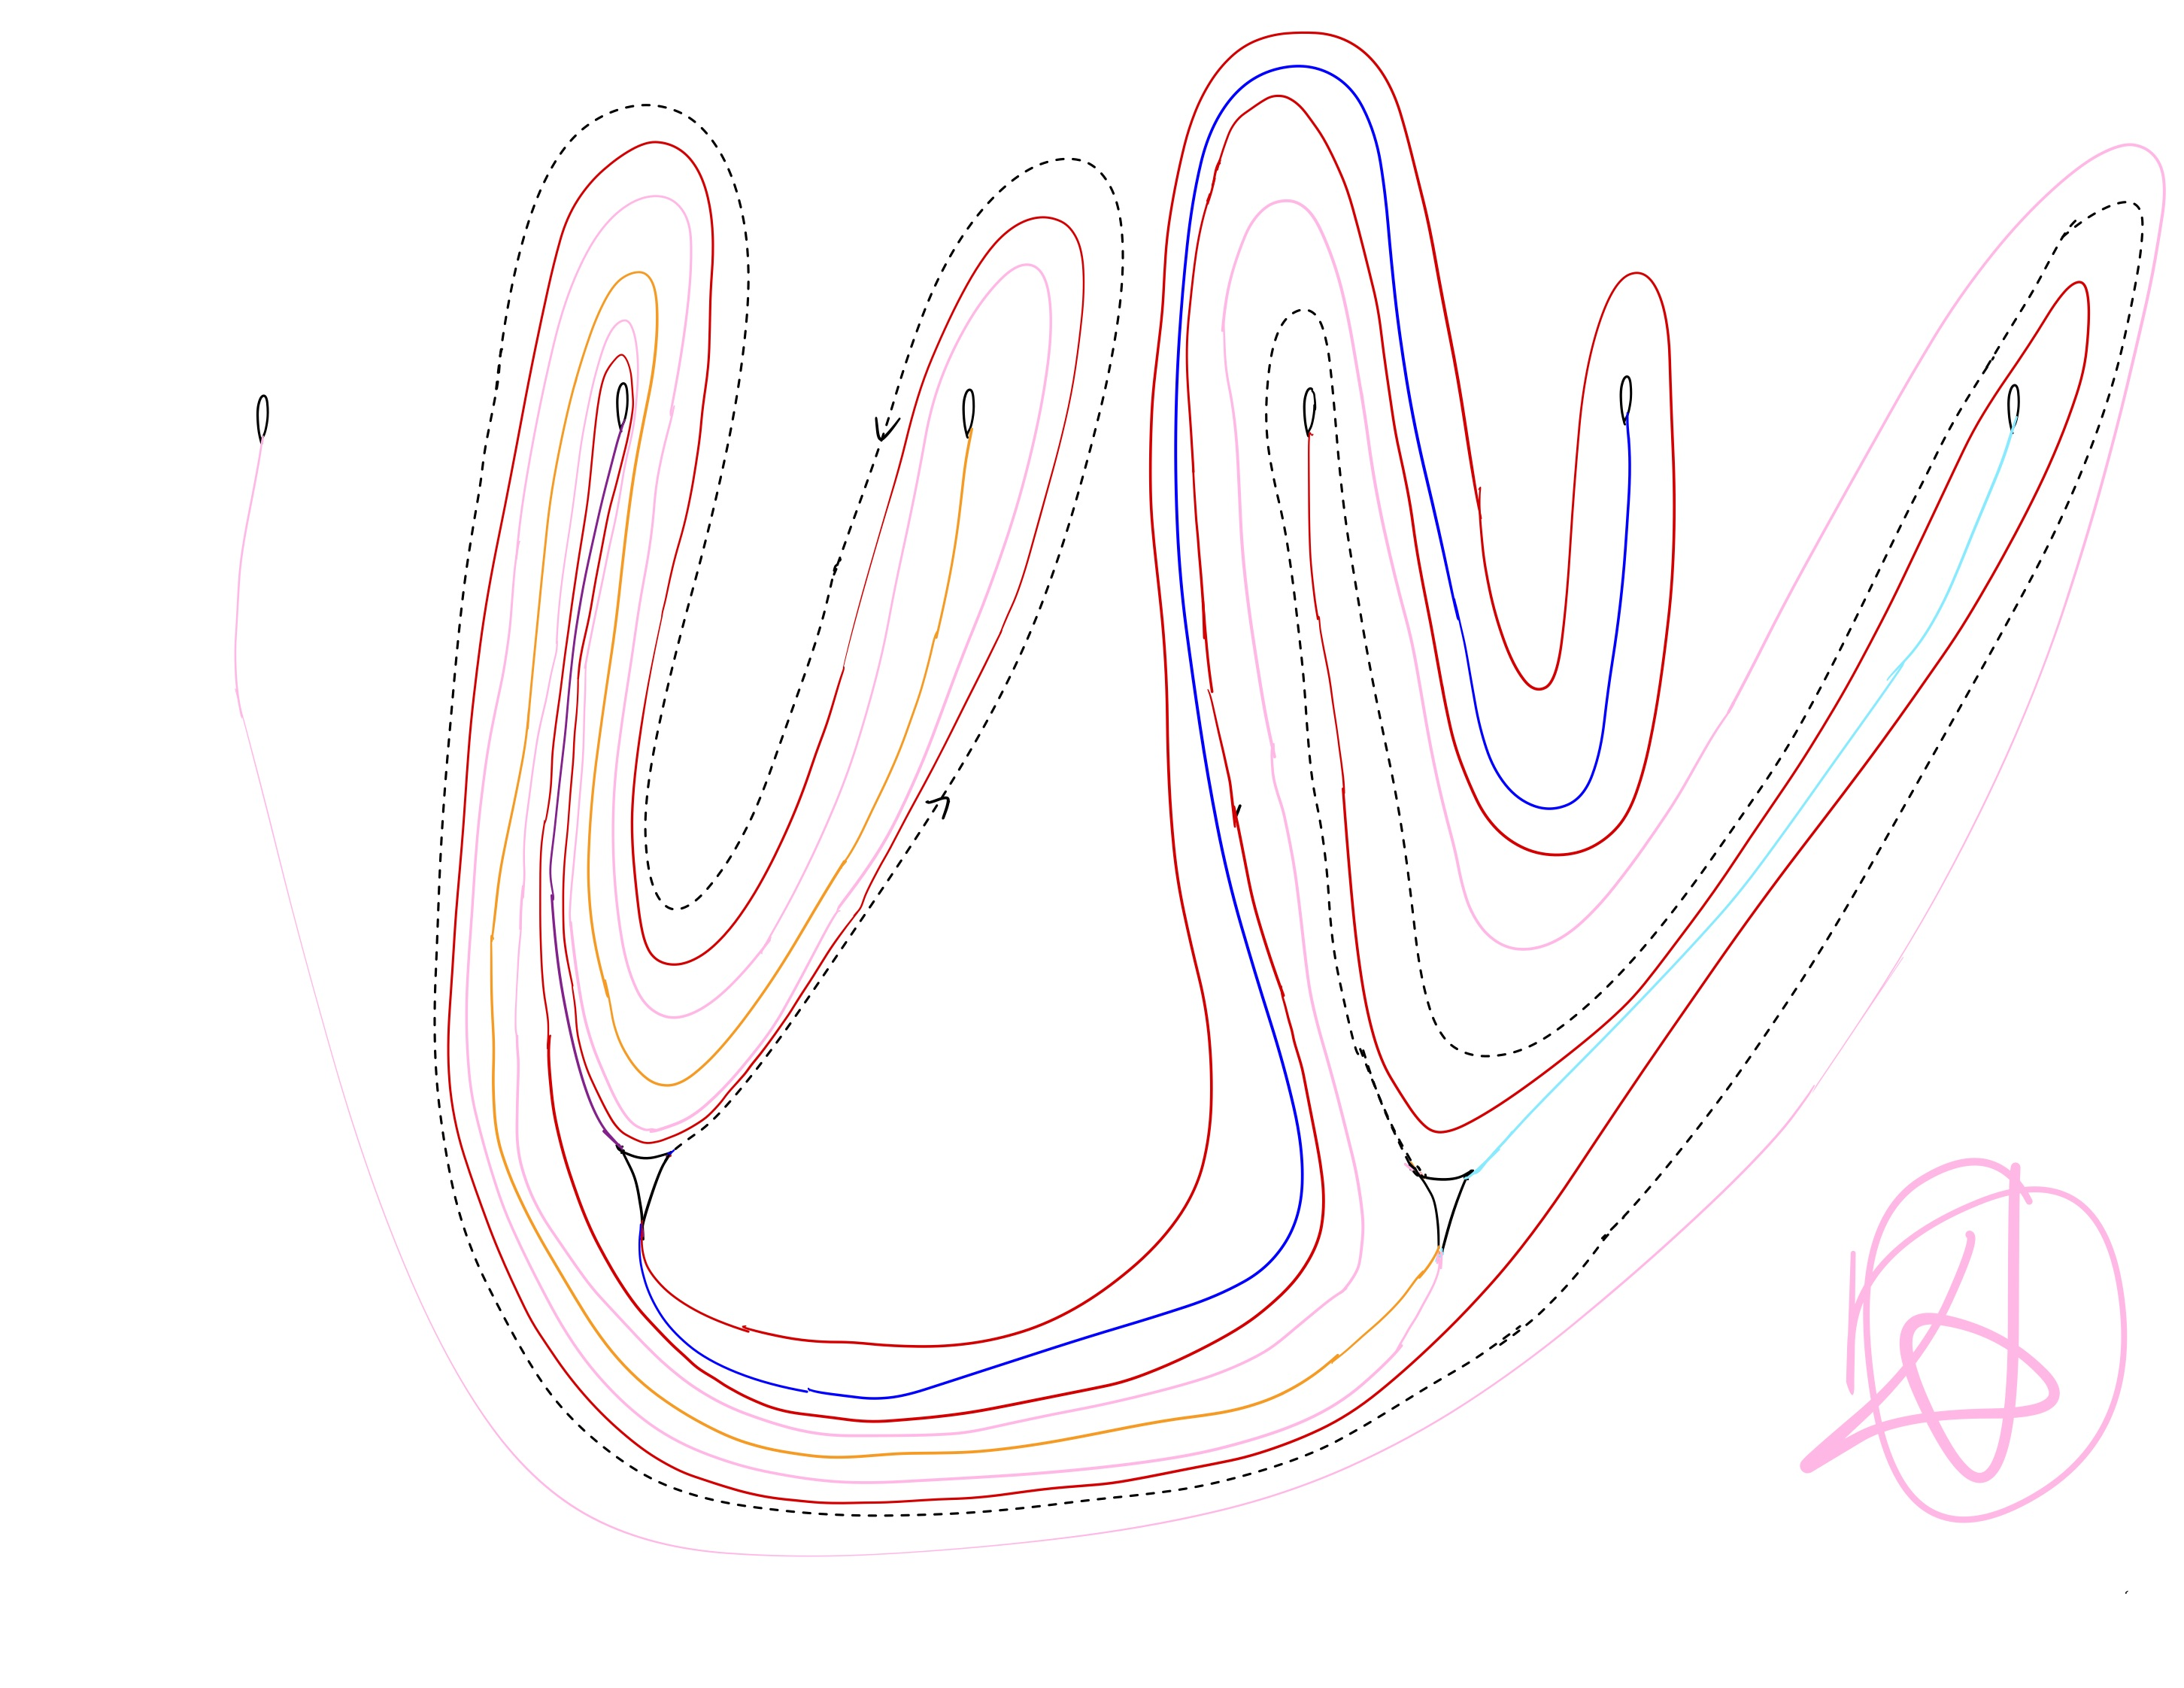
\includegraphics[width=\linewidth, height=0.45\textheight, keepaspectratio]{figures_braid/figures_track_0/Track 0 Braid 6 Fiasco-1.jpg}
    \caption{Train Track Map Candidate Family 6 of Track 0.}
    \label{fig:track0_braid_b0_6_map}
\end{figure*}

The inverse of the following braid carries this family of train track maps:
\[
b_6^0 = \sigma_{4} \sigma_{2} \sigma_{5}^{-1} \sigma_{5}^{-1} \sigma_{3} \sigma_{2} \sigma_{1} \sigma_{3} \sigma_{2} \sigma_{4}^{-1} \sigma_{5}^{-1} \sigma_{3} \sigma_{2} \sigma_{1} \sigma_{4} \sigma_{5} \sigma_{5}
\]

This is shown in Figure \ref{fig:track0_braid_b0_6}.

\begin{figure*}[p]
    \centering
    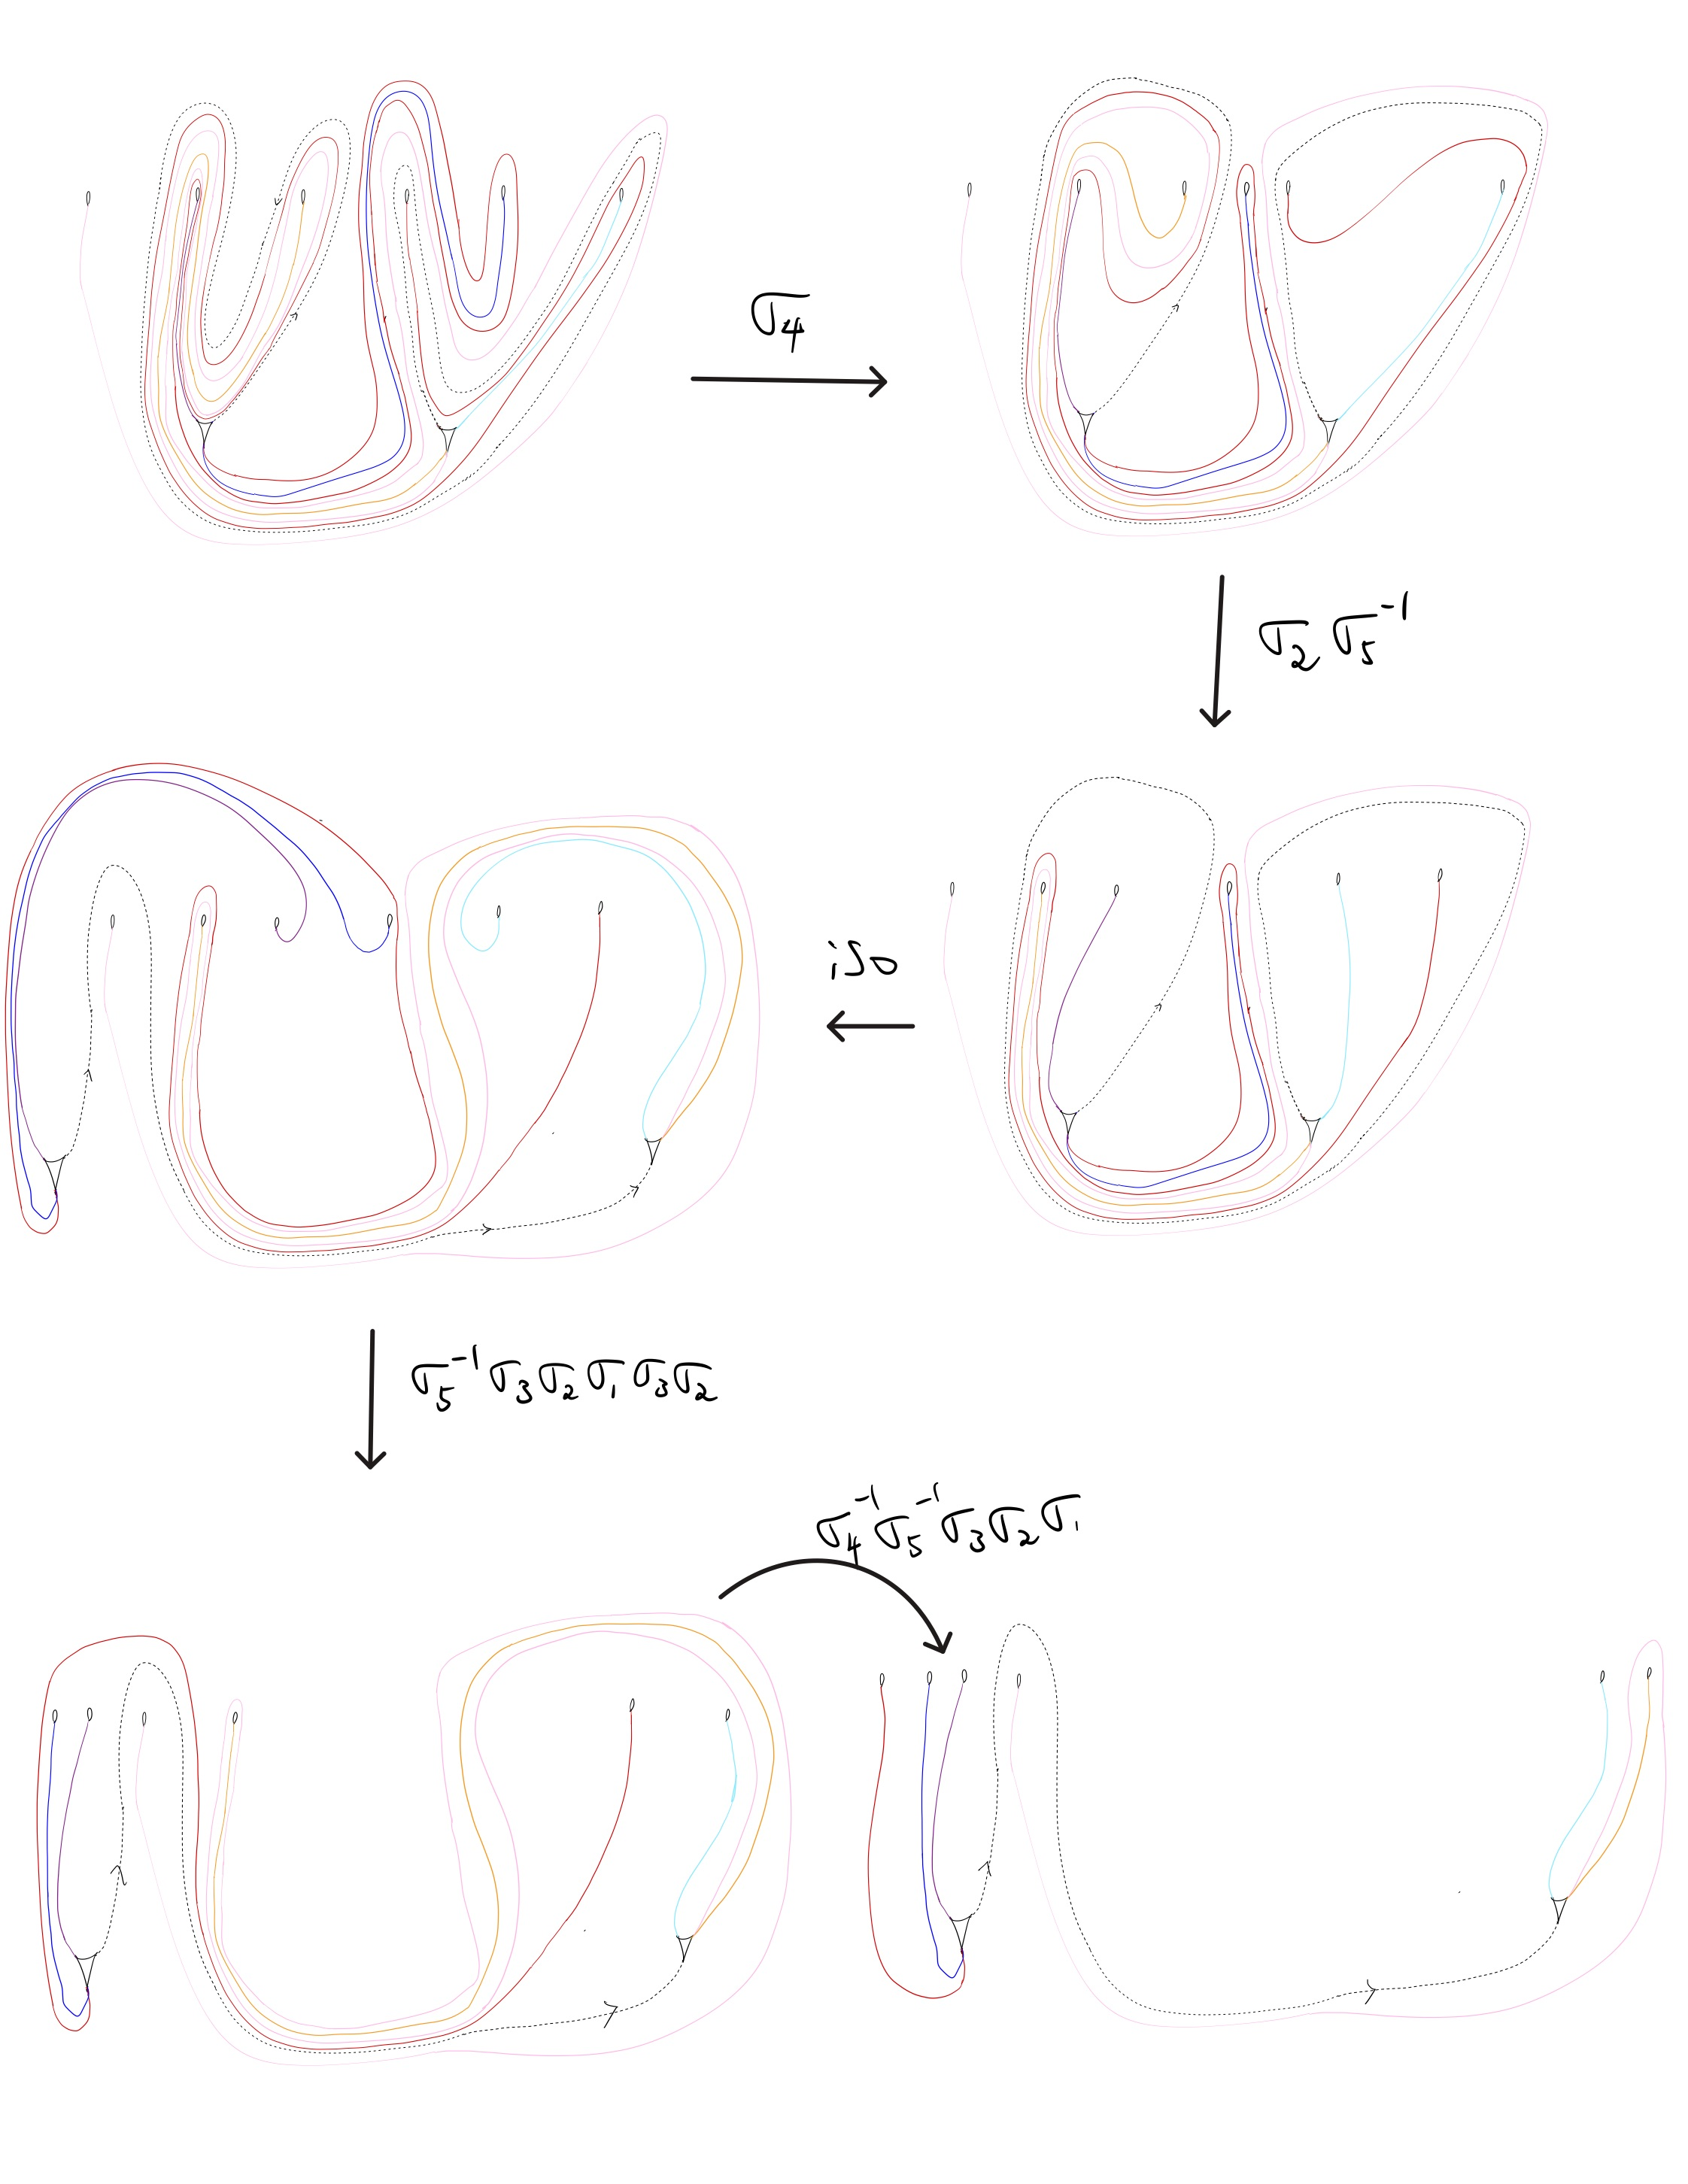
\includegraphics[width=\linewidth, height=0.45\textheight, keepaspectratio]{figures_braid/figures_track_0/Track 0 Braid 6 Fiasco-2.jpg}\\
    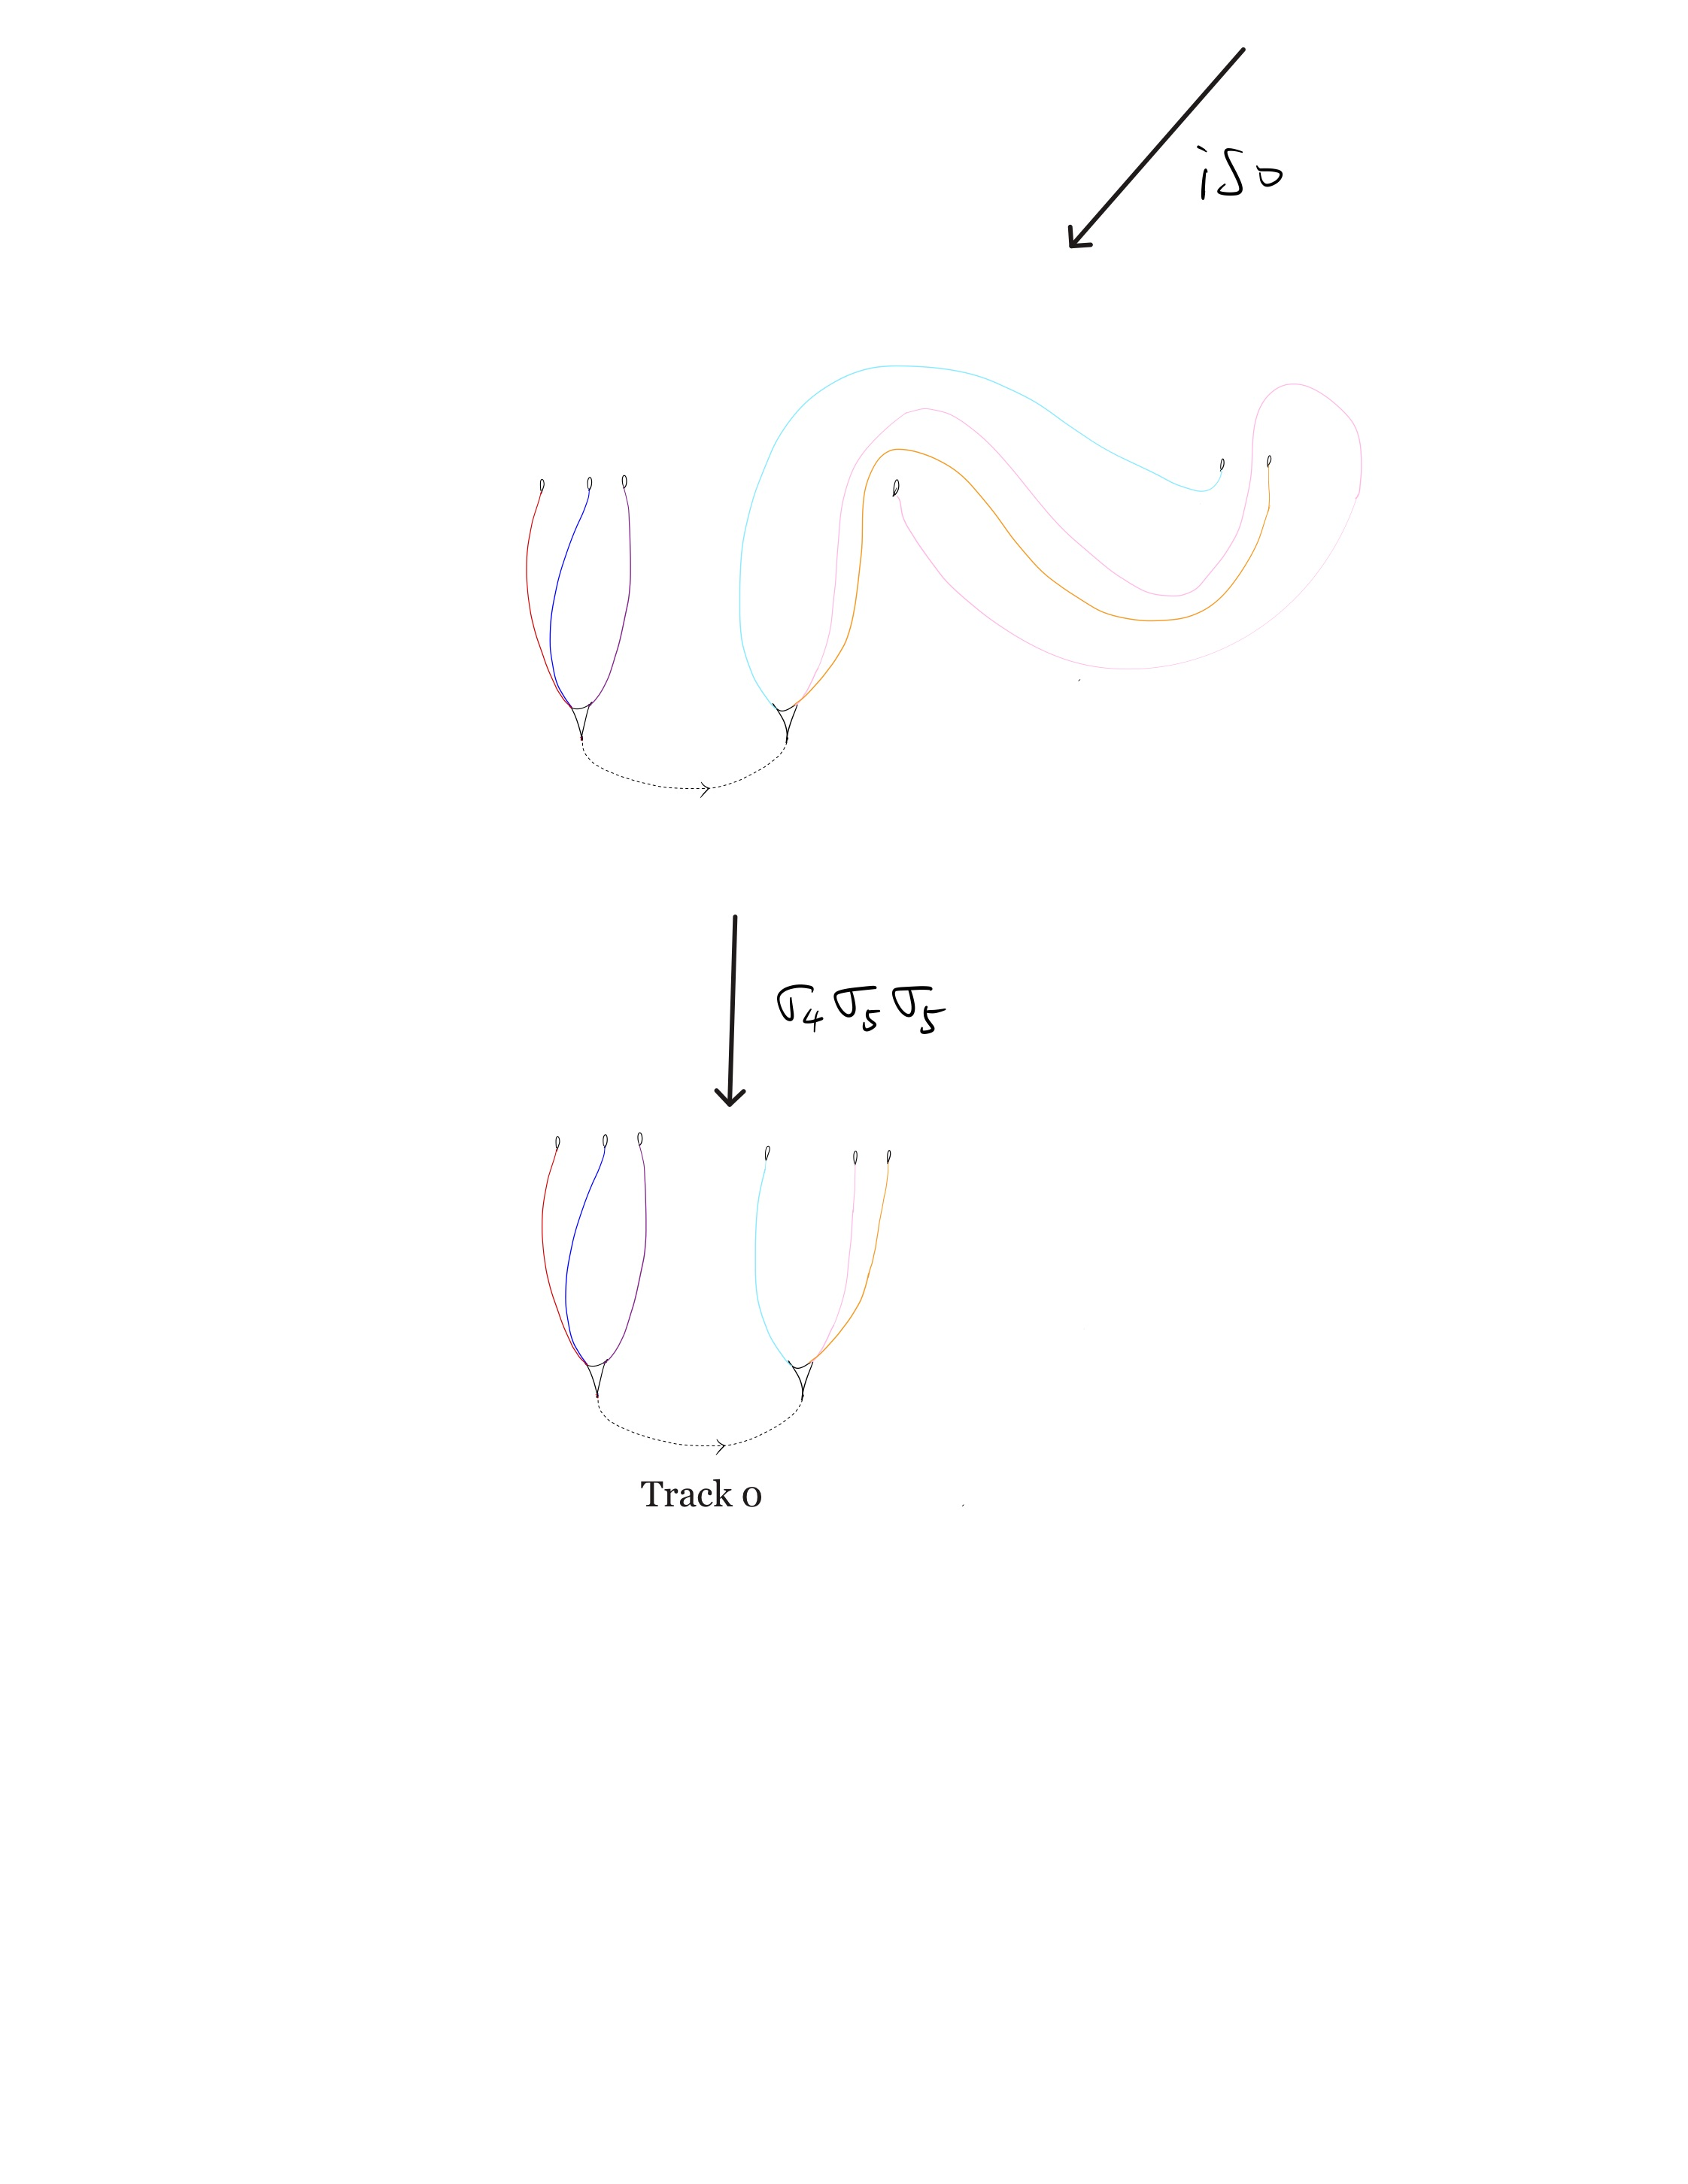
\includegraphics[width=\linewidth, height=0.45\textheight, keepaspectratio]{figures_braid/figures_track_0/Track 0 Braid 6 Fiasco-3.jpg}
    \caption{This sequence shows the inverse of the braid $b_6^0$ carries Train Track Candidate Family 6.}
    \label{fig:track0_braid_b0_6}
\end{figure*}

\clearpage

\section{Candidate Family 7 (Briefing)}\label{sec:track0_briefing_1}
Train Track Map Candidate Family 7 of Track 0 is shown in Figure \ref{fig:track0_braid_b0_7_map}. See \ref{Briefing} for details.

\begin{figure*}[ht]
    \centering
    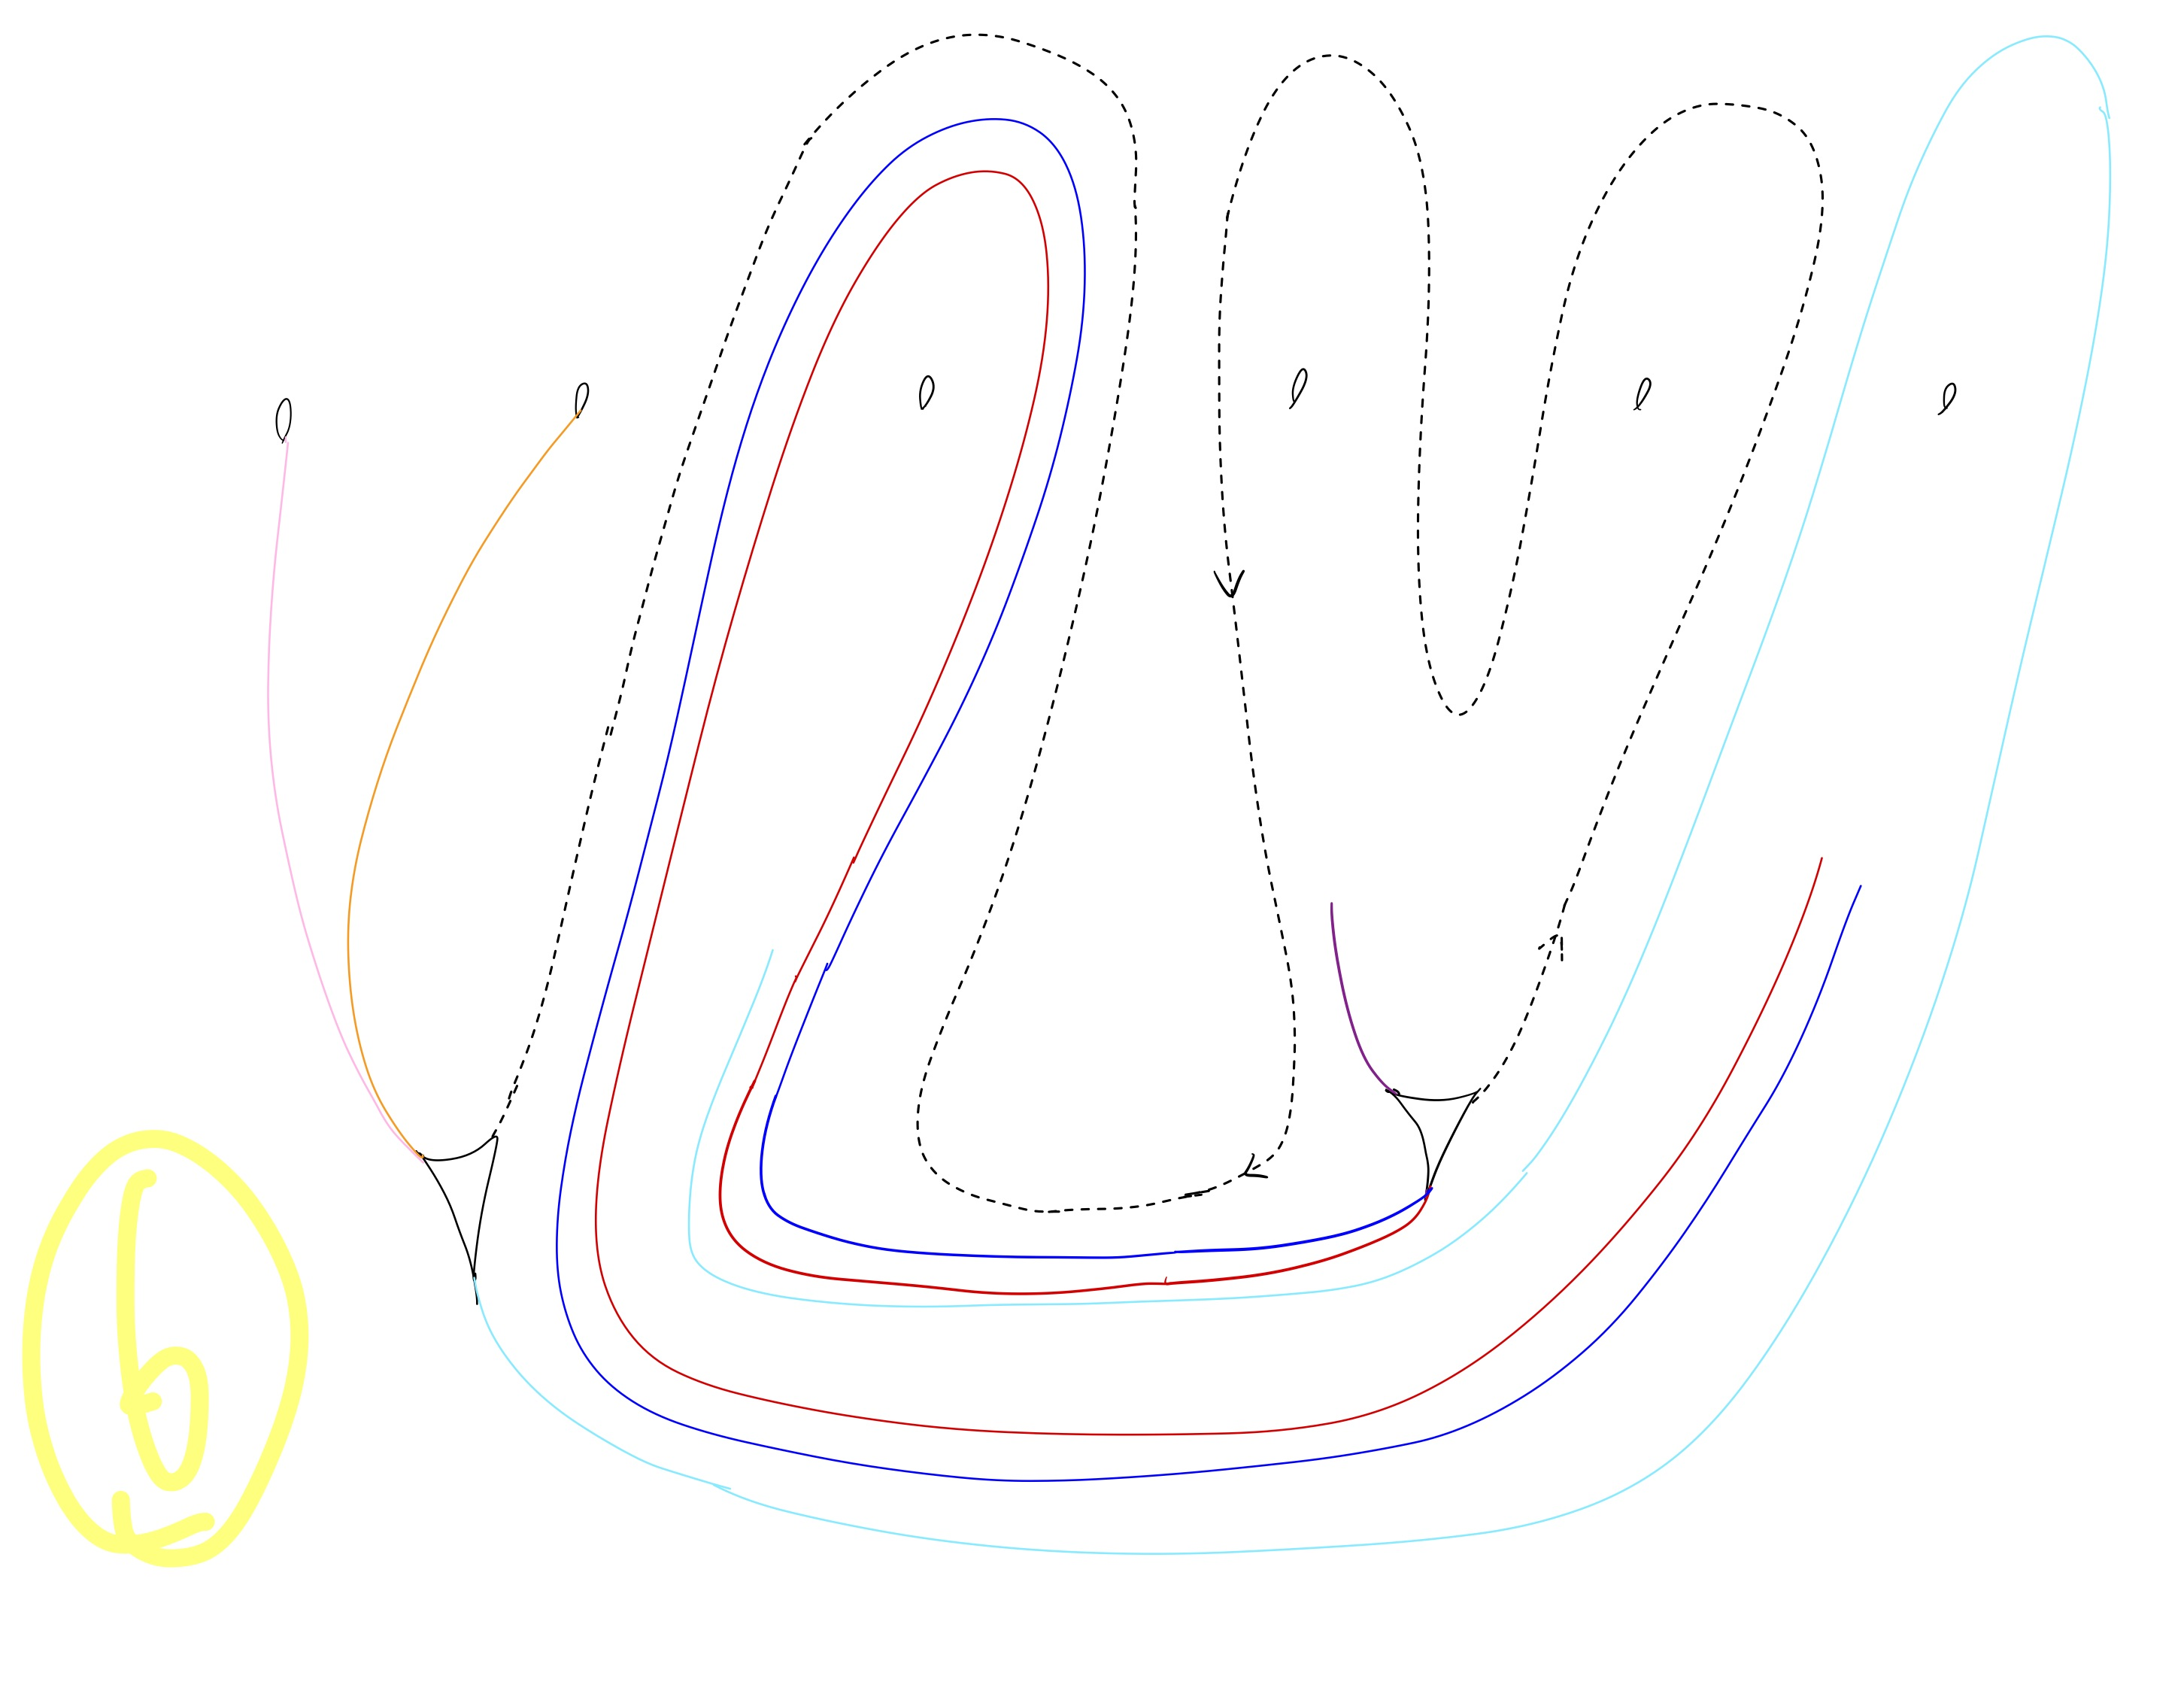
\includegraphics[width=\linewidth, height=0.45\textheight, keepaspectratio]{figures_braid/figures_track_0/Track 0 Braid 7 Briefing-2.jpg}
    \caption{Train Track Map Candidate Family 7 of Track 0.}
    \label{fig:track0_braid_b0_7_map}
\end{figure*}

The inverse of the following braid carries this family of train track maps:
\[
b_7^0 = \sigma_{4}^m \sigma_{3} \sigma_{4} \sigma_{5}^{-k} \sigma_{3} \sigma_{3} \sigma_{4}^j \sigma_{4} \sigma_{3} \sigma_{2} \sigma_{1} \sigma_{4} \sigma_{3} \sigma_{2} \sigma_{4} \sigma_{3} \sigma_{5} \sigma_{4} \sigma_{5} \sigma_{5}
\]
where $m, k, j \geq 1$ ($m, k, j \in \mathbb{Z}$) are the twisting parameters. This is shown in Figure \ref{fig:track0_braid_b0_7}.

\begin{figure*}[p]
    \centering
    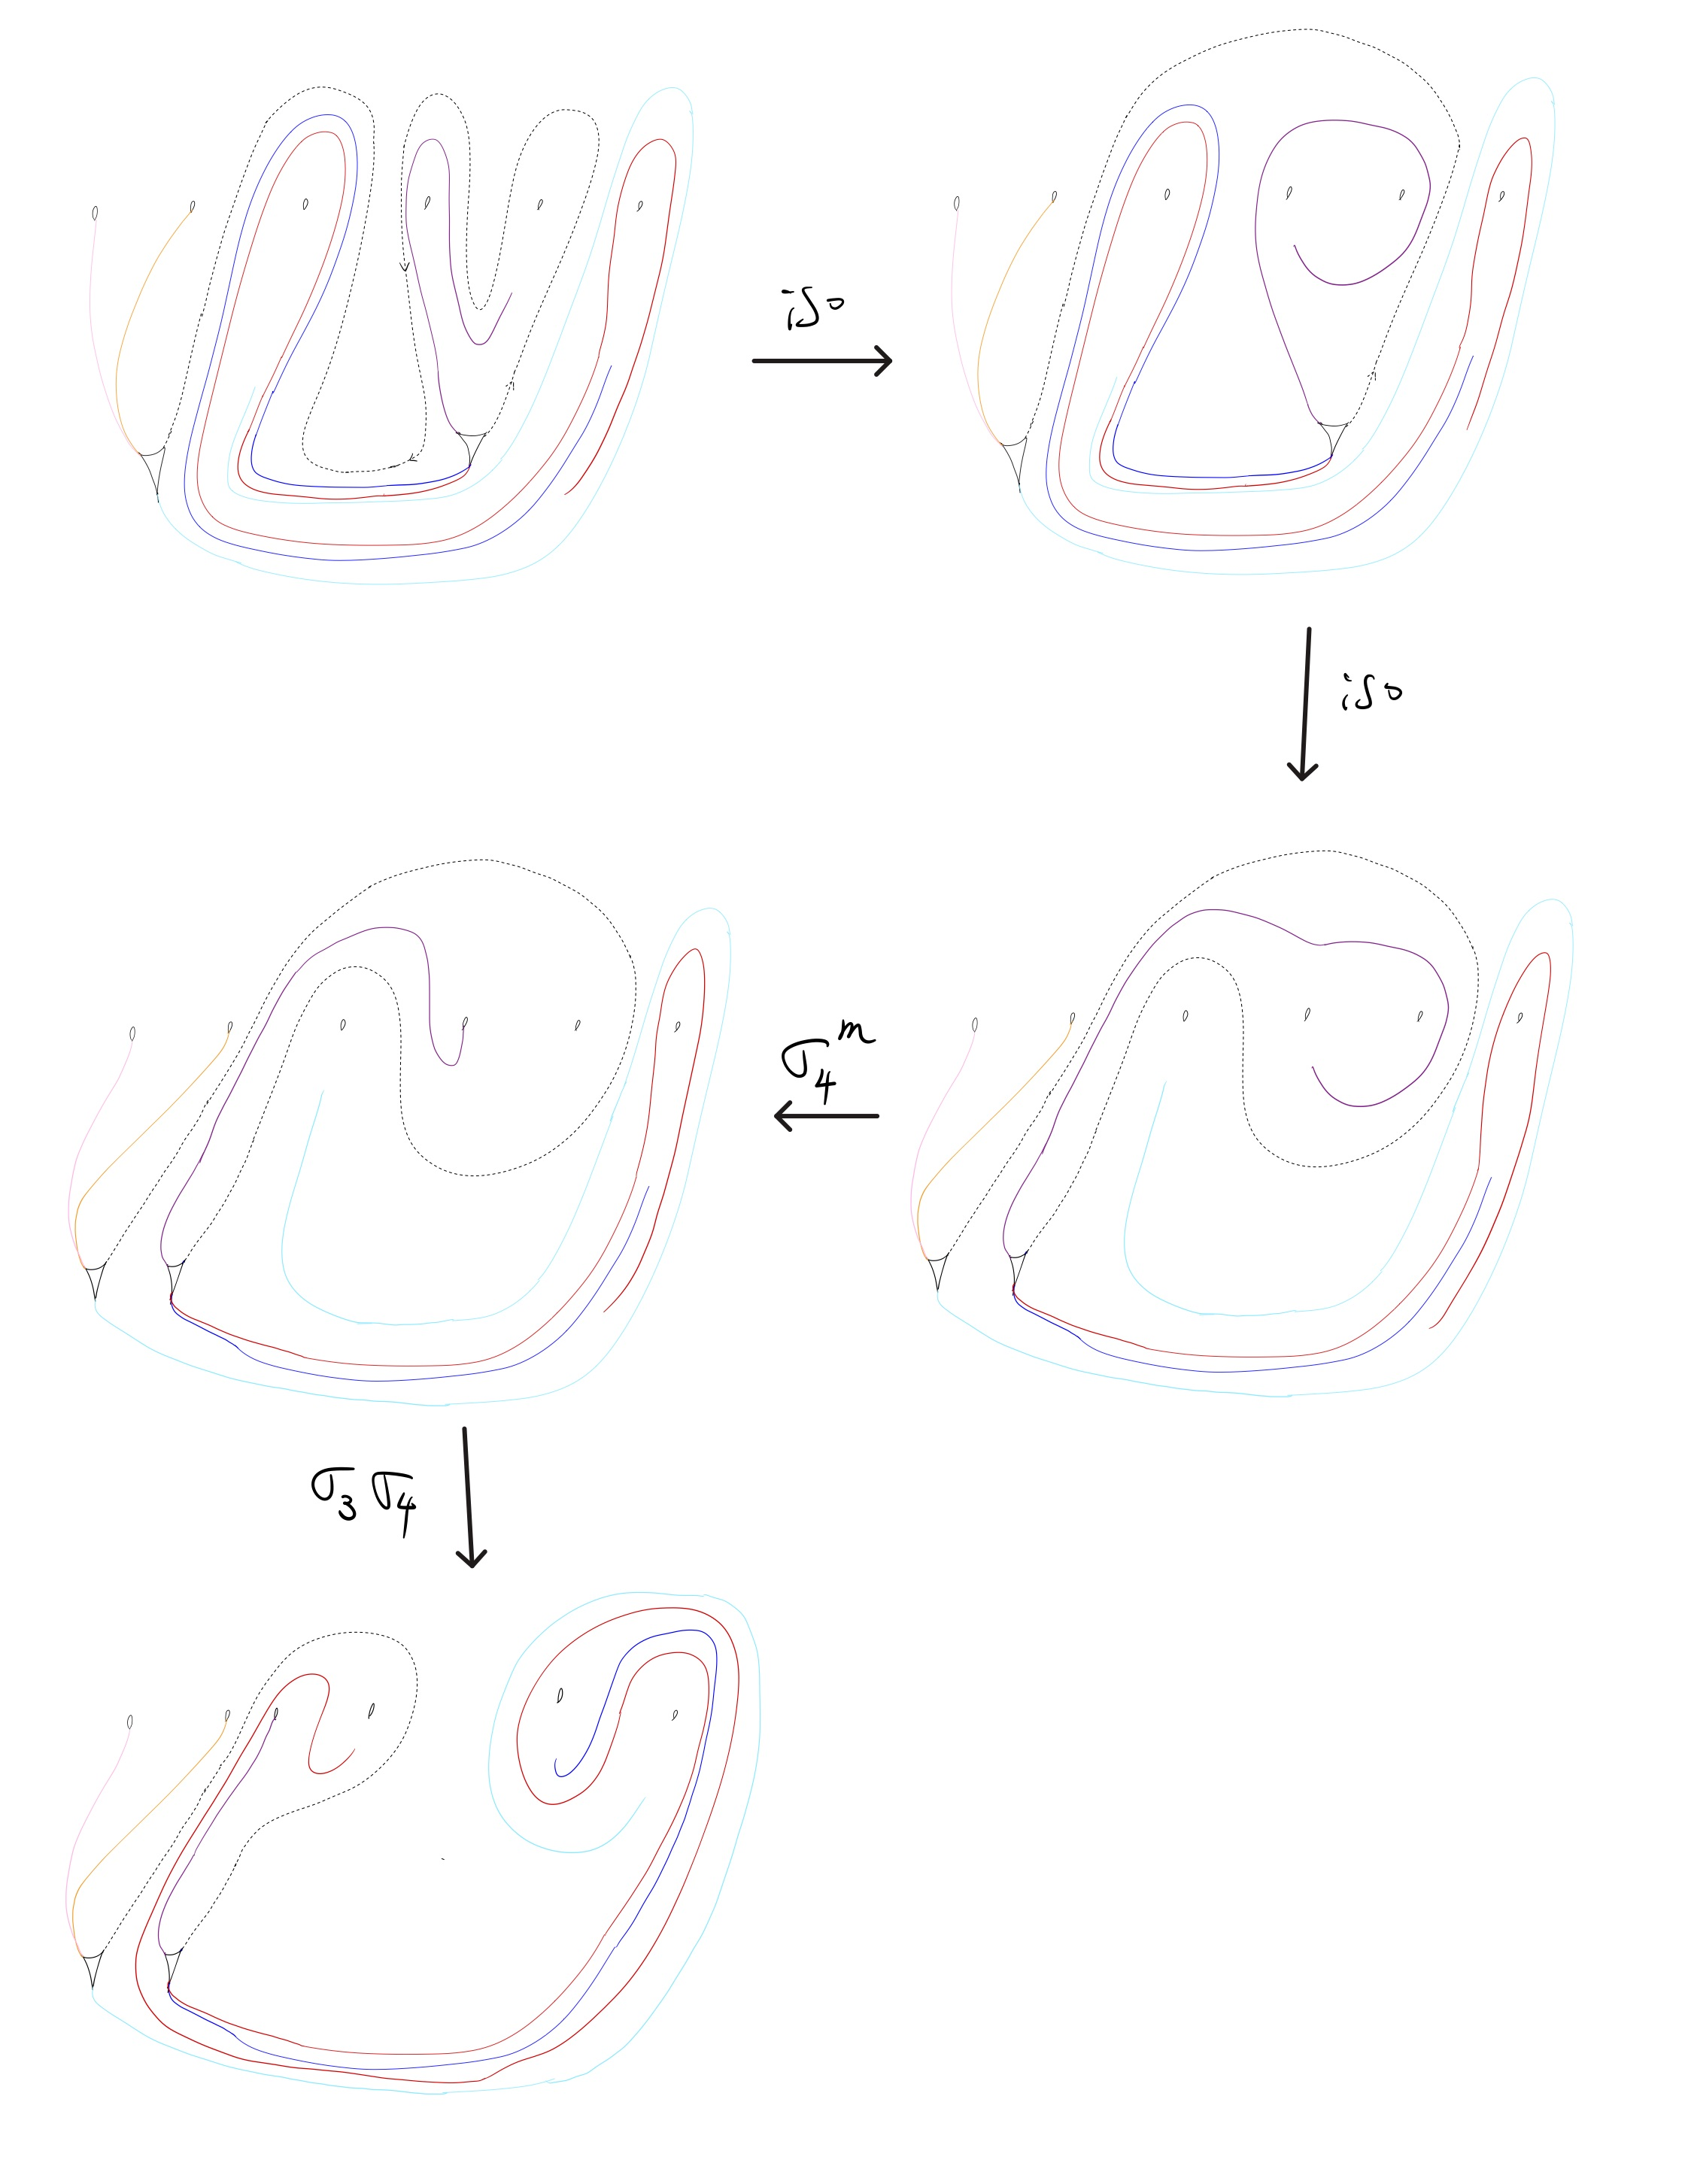
\includegraphics[width=\linewidth, height=0.45\textheight, keepaspectratio]{figures_braid/figures_track_0/Track 0 Braid 7 Briefing-3.jpg}\\
    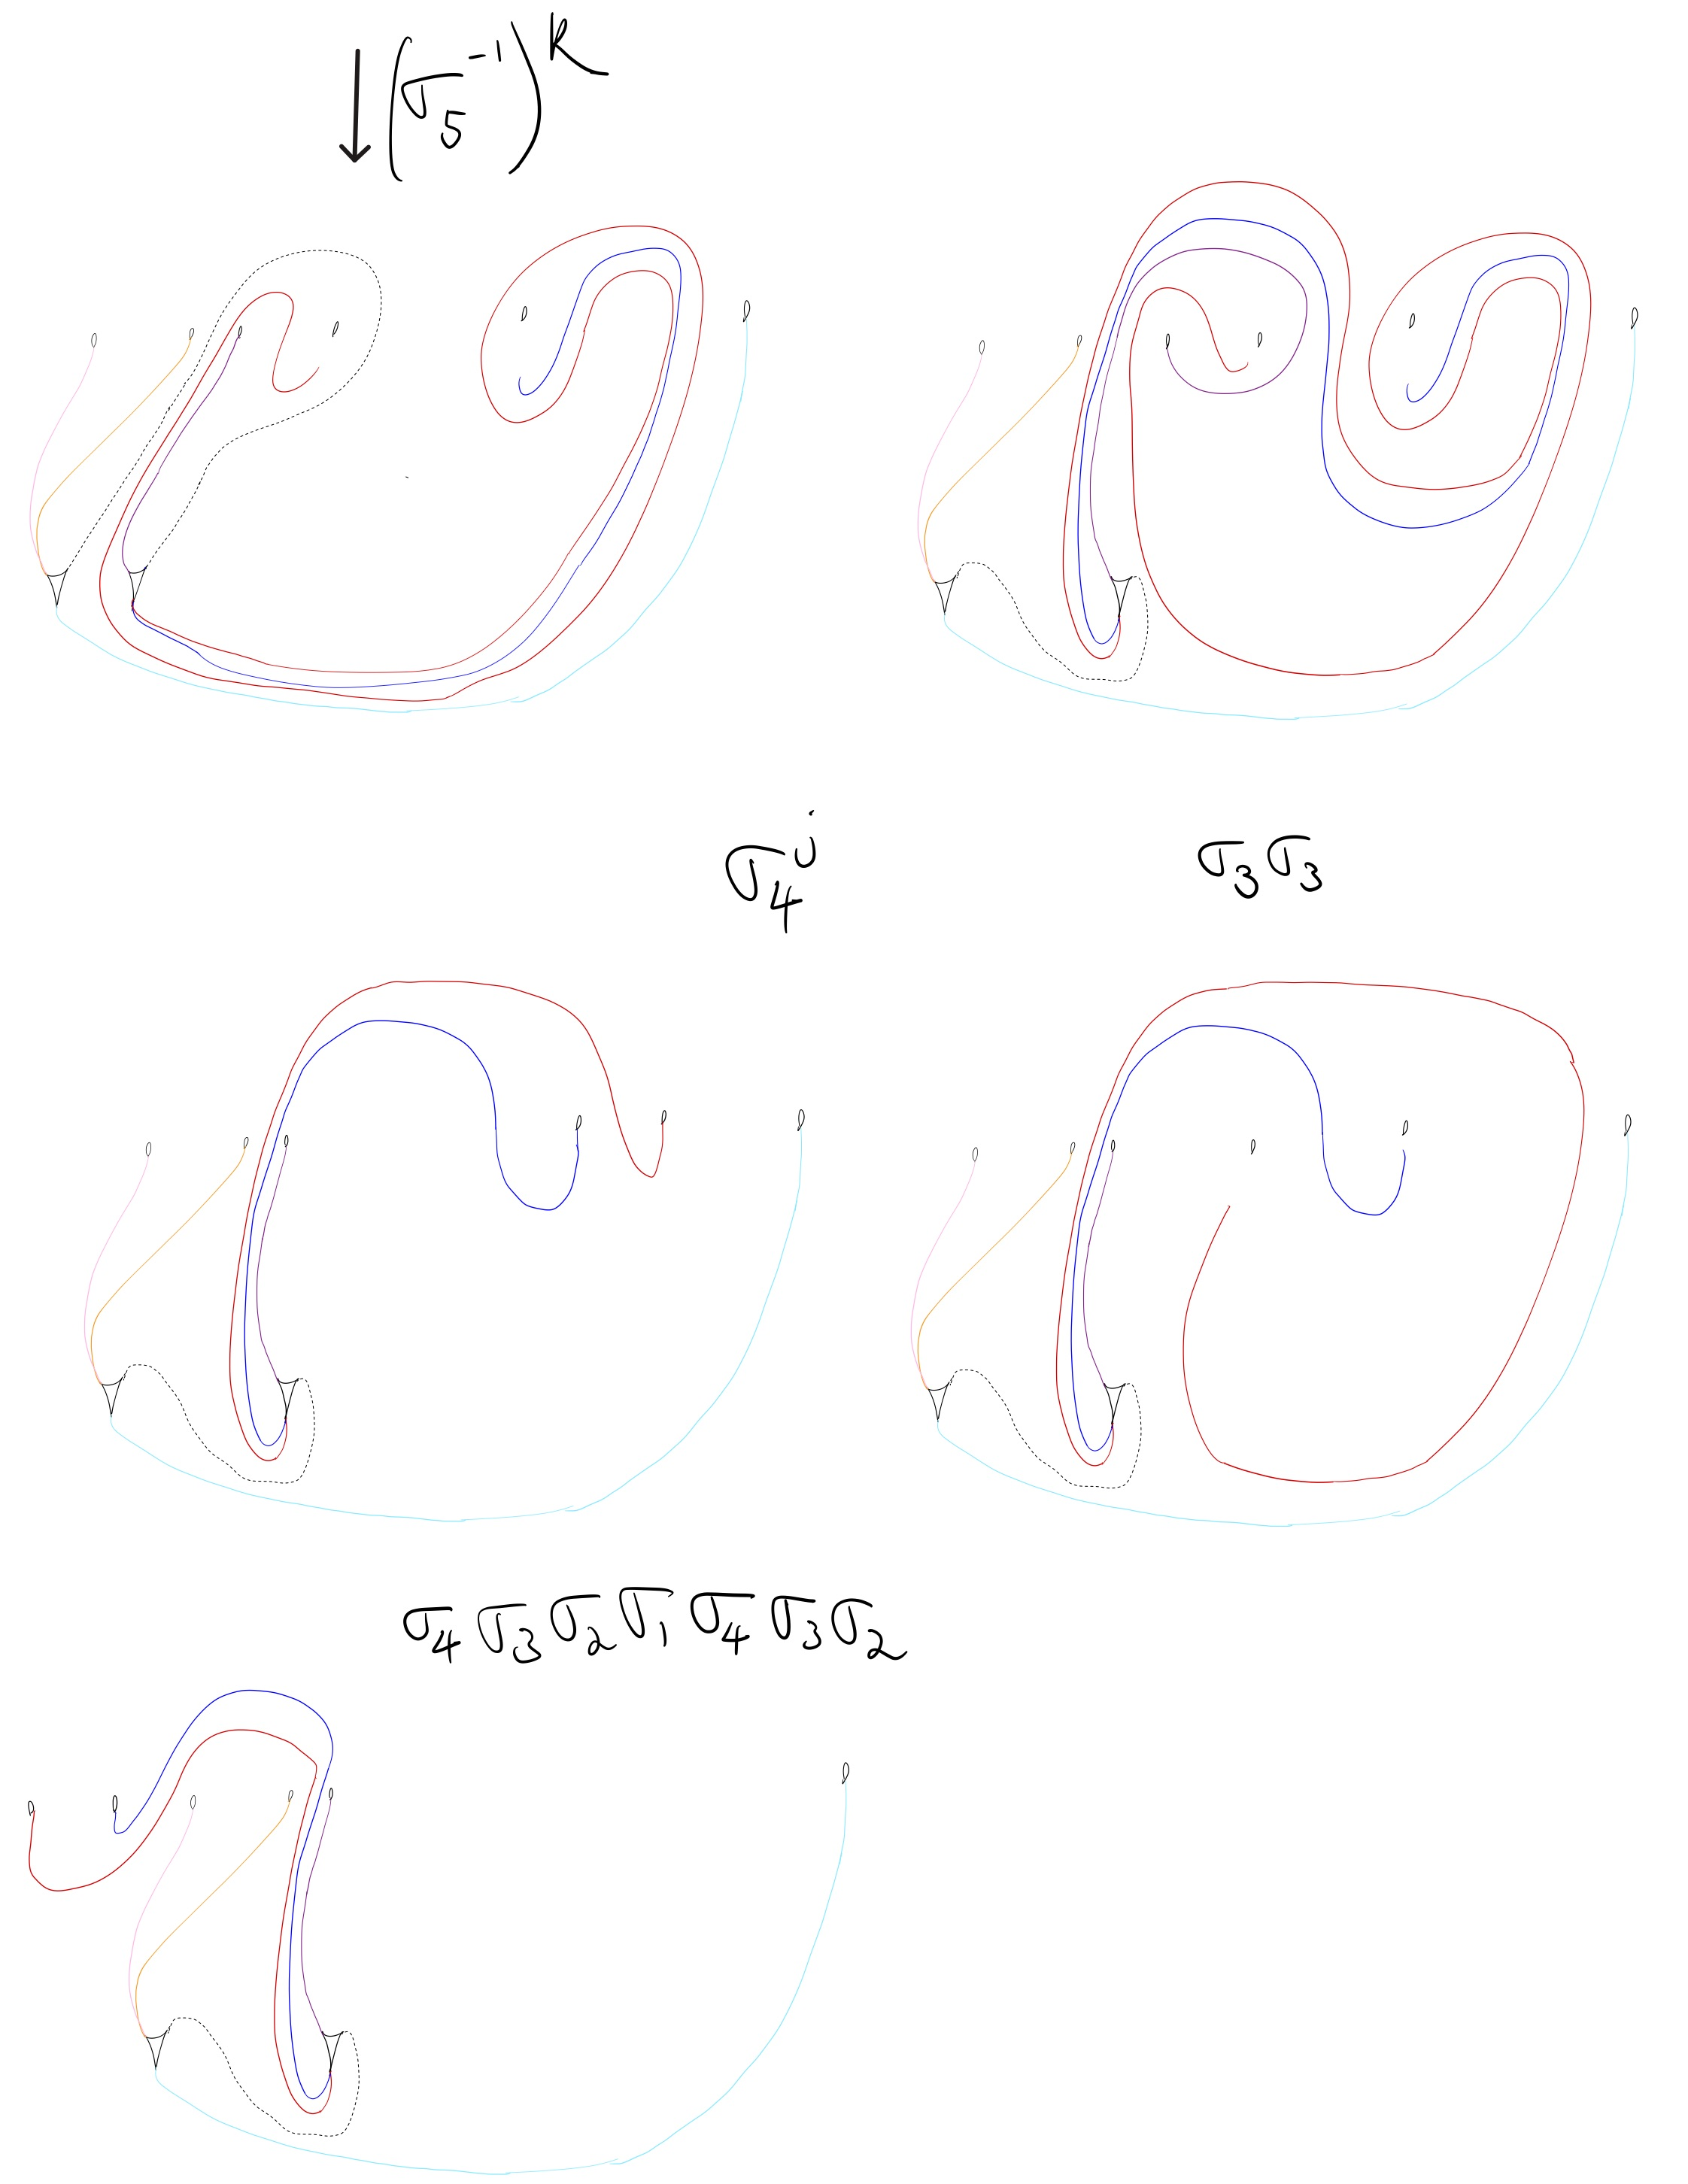
\includegraphics[width=\linewidth, height=0.45\textheight, keepaspectratio]{figures_braid/figures_track_0/Track 0 Braid 7 Briefing-4.jpg}
    \caption{This sequence shows the inverse of the braid $b_7^0$ carries Train Track Candidate Family 7.}
    \label{fig:track0_braid_b0_7}
\end{figure*}

\begin{figure*}[p]
    \ContinuedFloat
    \centering
    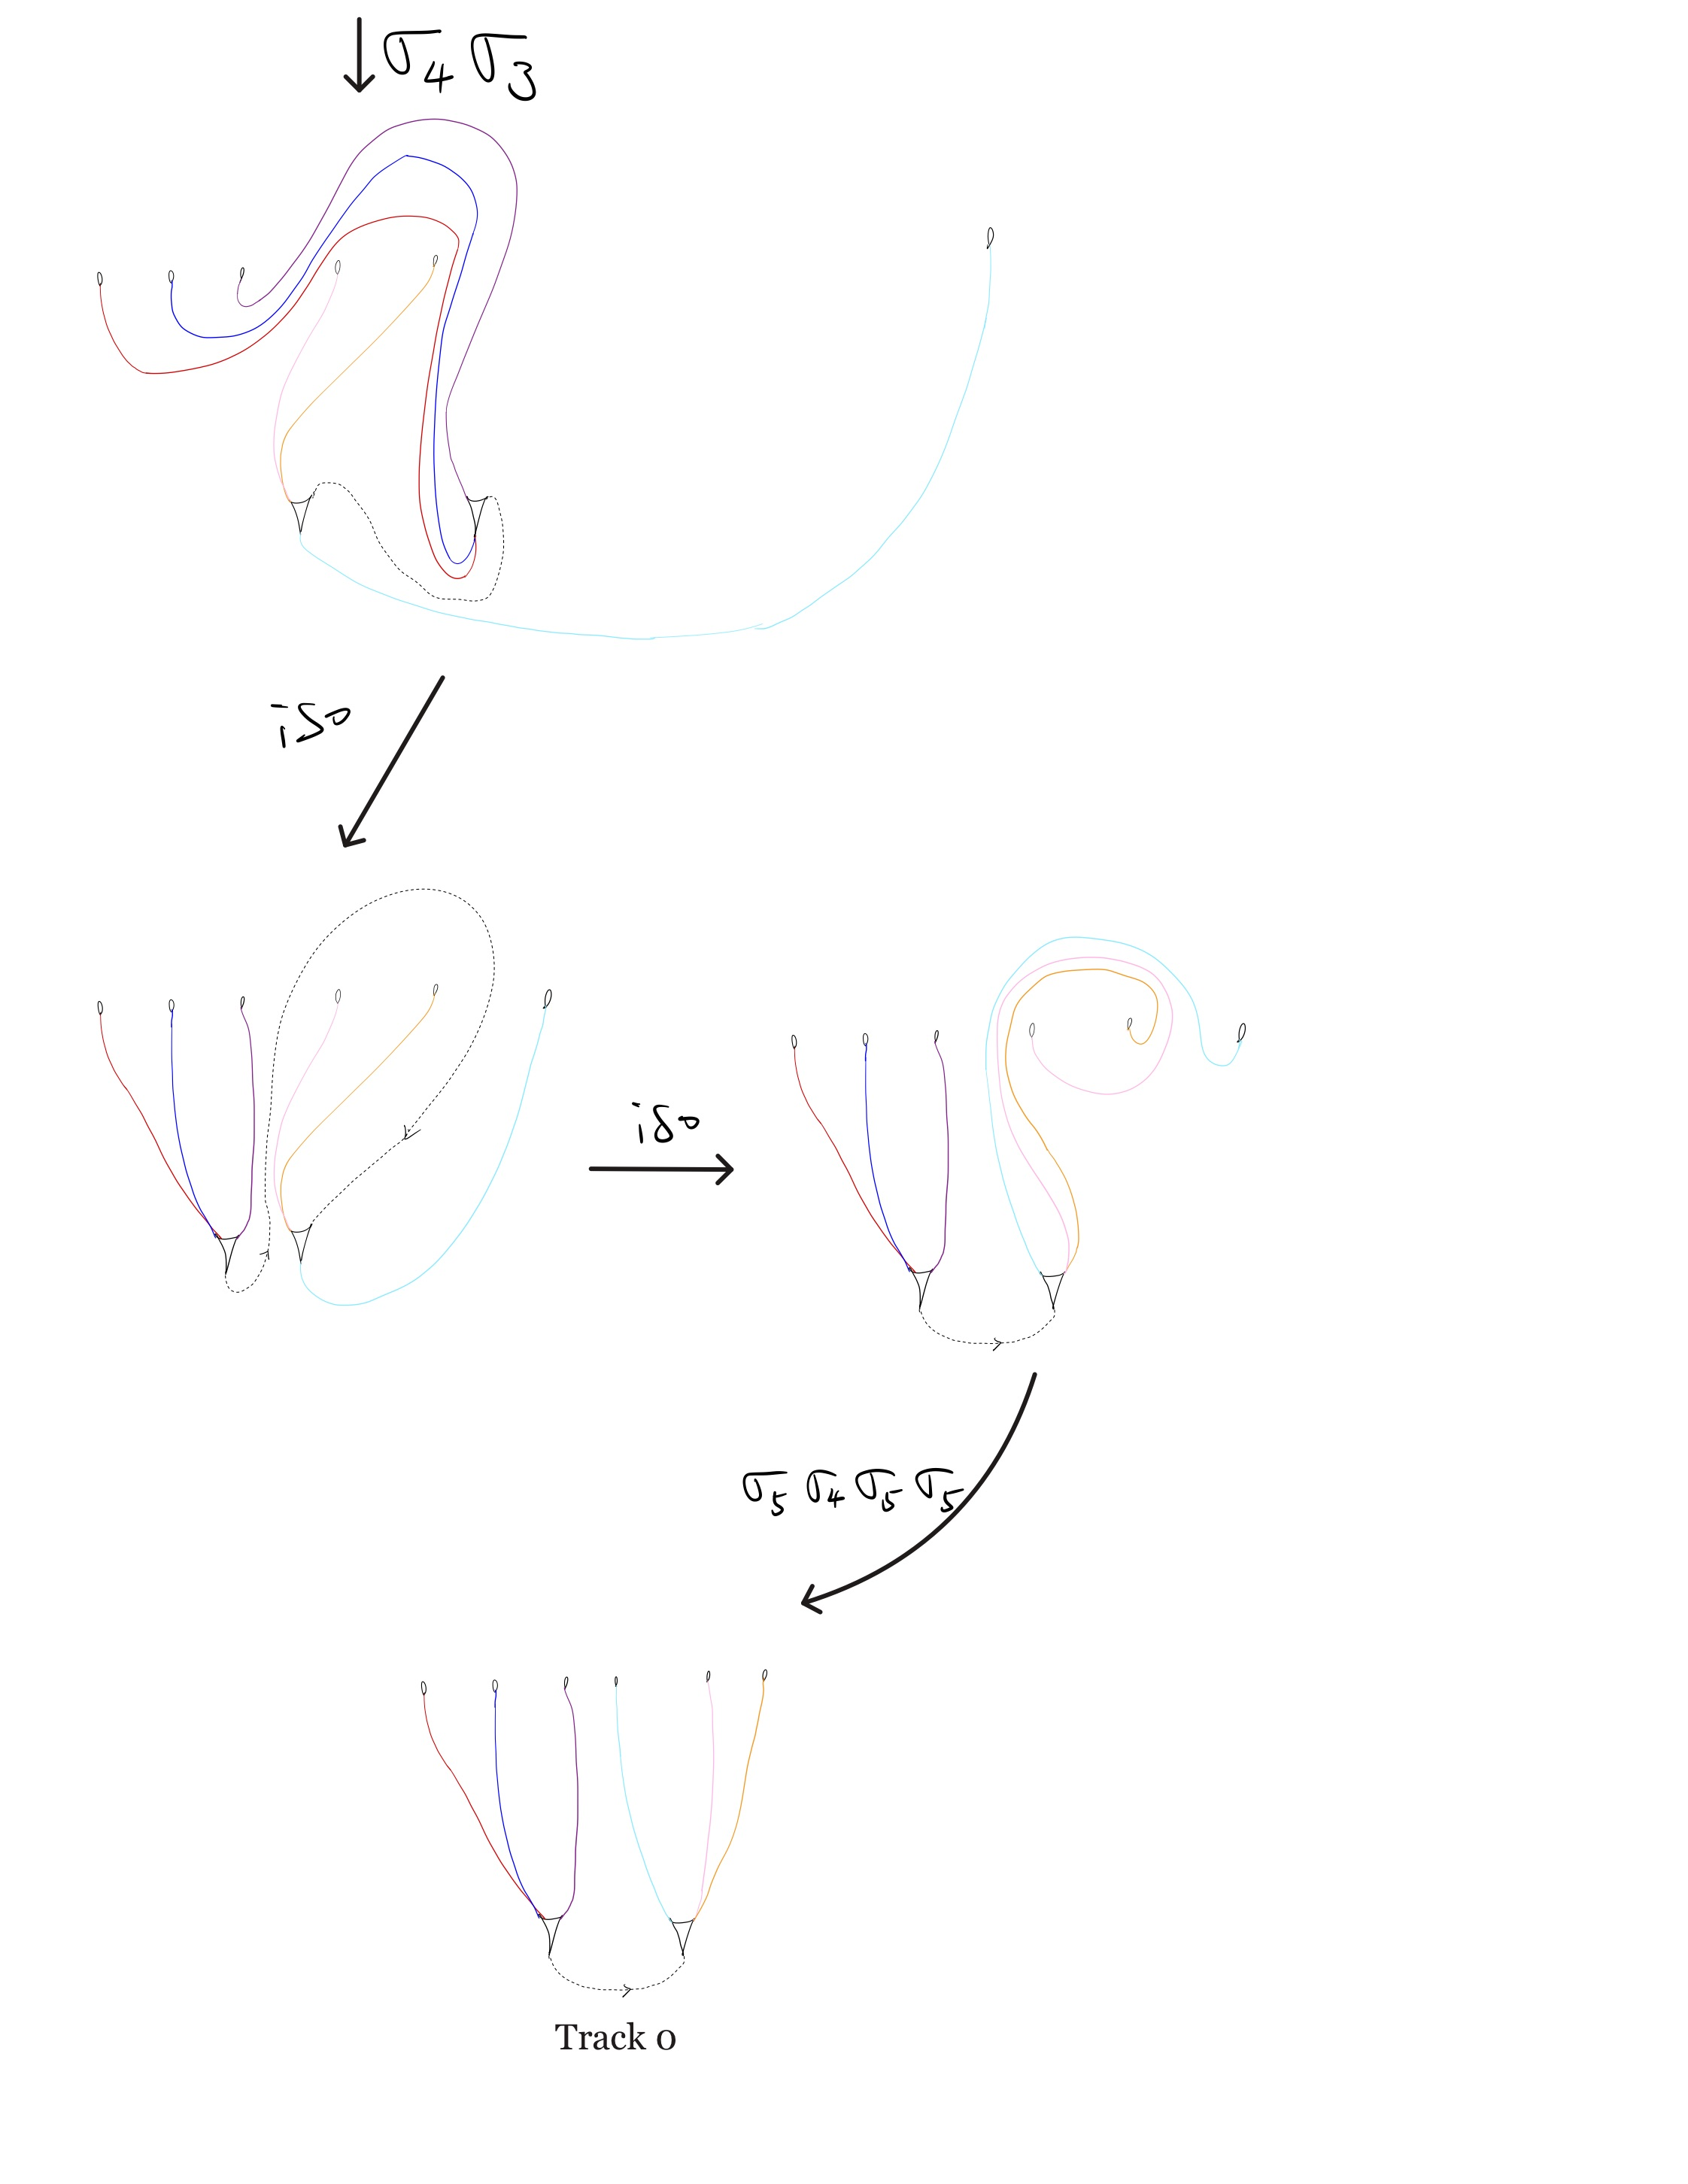
\includegraphics[width=\linewidth, height=0.45\textheight, keepaspectratio]{figures_braid/figures_track_0/Track 0 Braid 7 Briefing-5.jpg}
    \caption[]{This sequence shows the inverse of the braid $b_7^0$ carries Train Track Candidate Family 7 (continued).}
\end{figure*}

\clearpage

\section{Candidate Family 8 (Briefing)}\label{sec:track0_briefing_2}
Train Track Map Candidate Family 8 of Track 0 is shown in Figure \ref{fig:track0_braid_b0_8_map}. See \ref{Briefing} for details.

\begin{figure*}[ht]
    \centering
    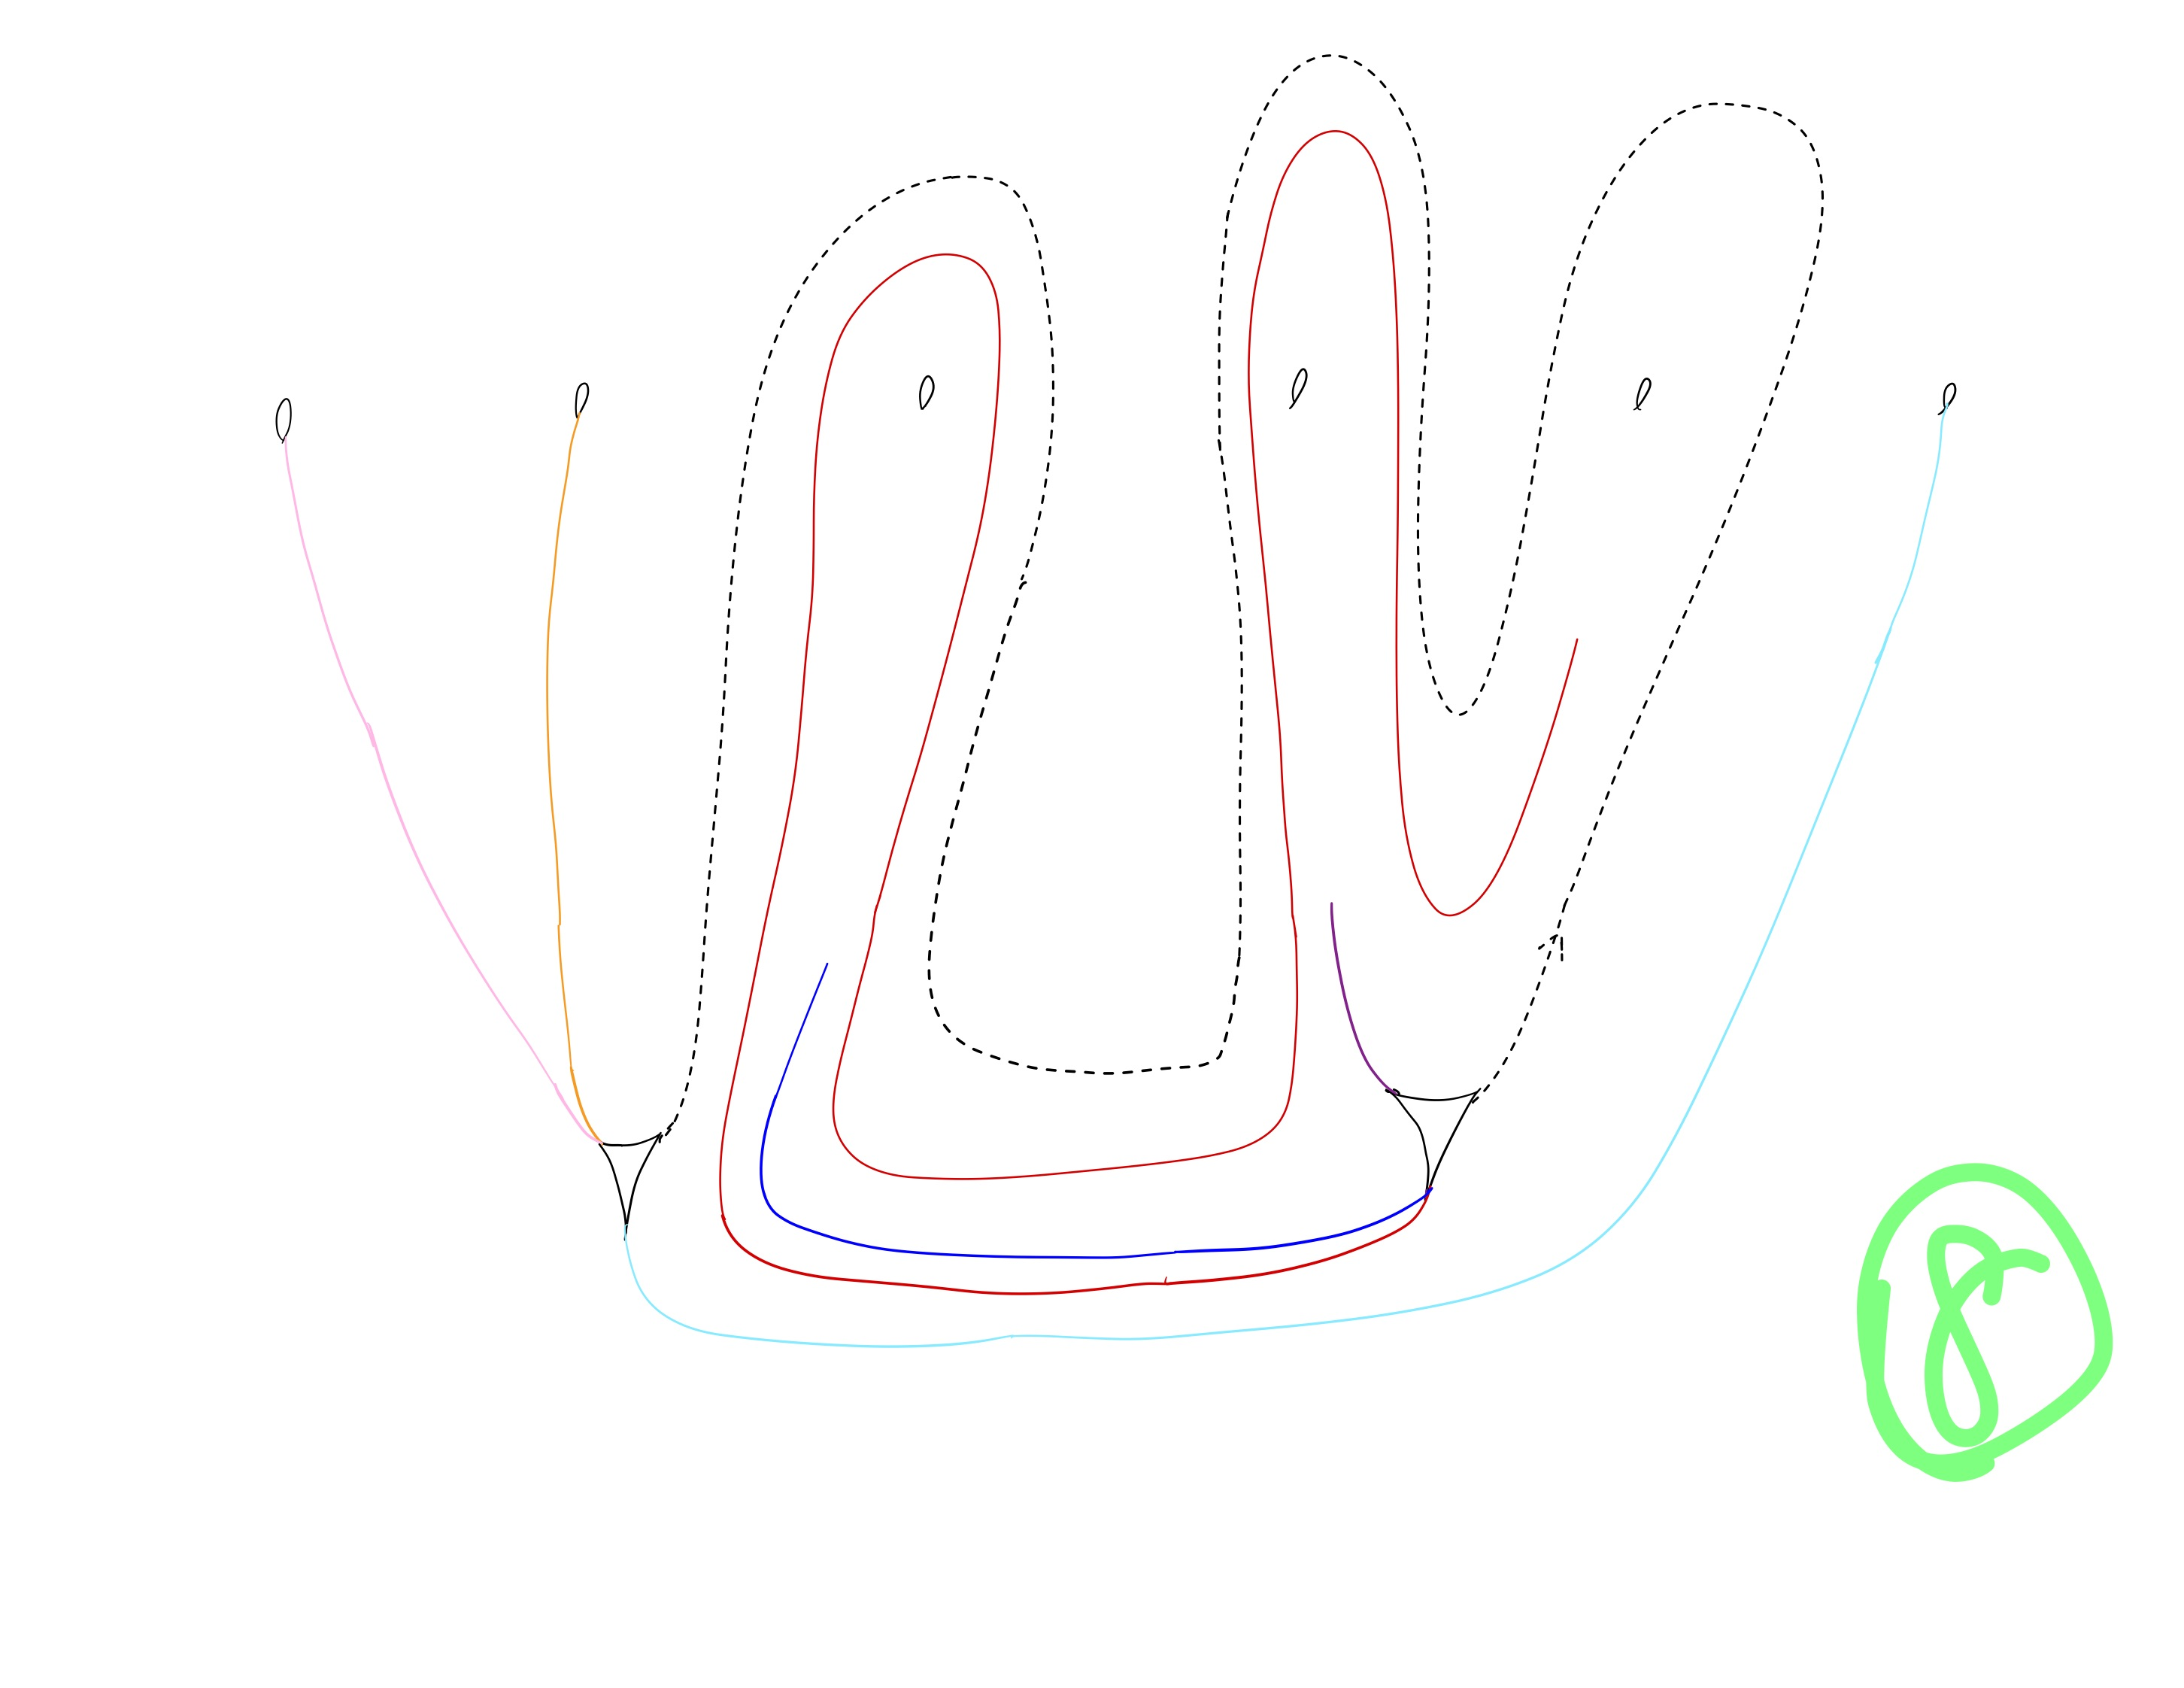
\includegraphics[width=\linewidth, height=0.45\textheight, keepaspectratio]{figures_braid/figures_track_0/Track 0 Braid 8 Briefing-1.jpg}
    \caption{Train Track Map Candidate Family 8 of Track 0.}
    \label{fig:track0_braid_b0_8_map}
\end{figure*}

The inverse of the following braid carries this family of train track maps:
\[
b_8^0 = \sigma_{4}^k \sigma_{3}^m \sigma_{3} \sigma_{4} \sigma_{4} \sigma_{3} \sigma_{4} \sigma_{4} \sigma_{2} \sigma_{1} \sigma_{3} \sigma_{2} \sigma_{4} \sigma_{3} \sigma_{5} \sigma_{4} \sigma_{5} \sigma_{5}
\]
where $k, m \geq 1$ ($k, m \in \mathbb{Z}$) are the twisting parameters. This is shown in Figure \ref{fig:track0_braid_b0_8}.

\begin{figure*}[p]
    \centering
    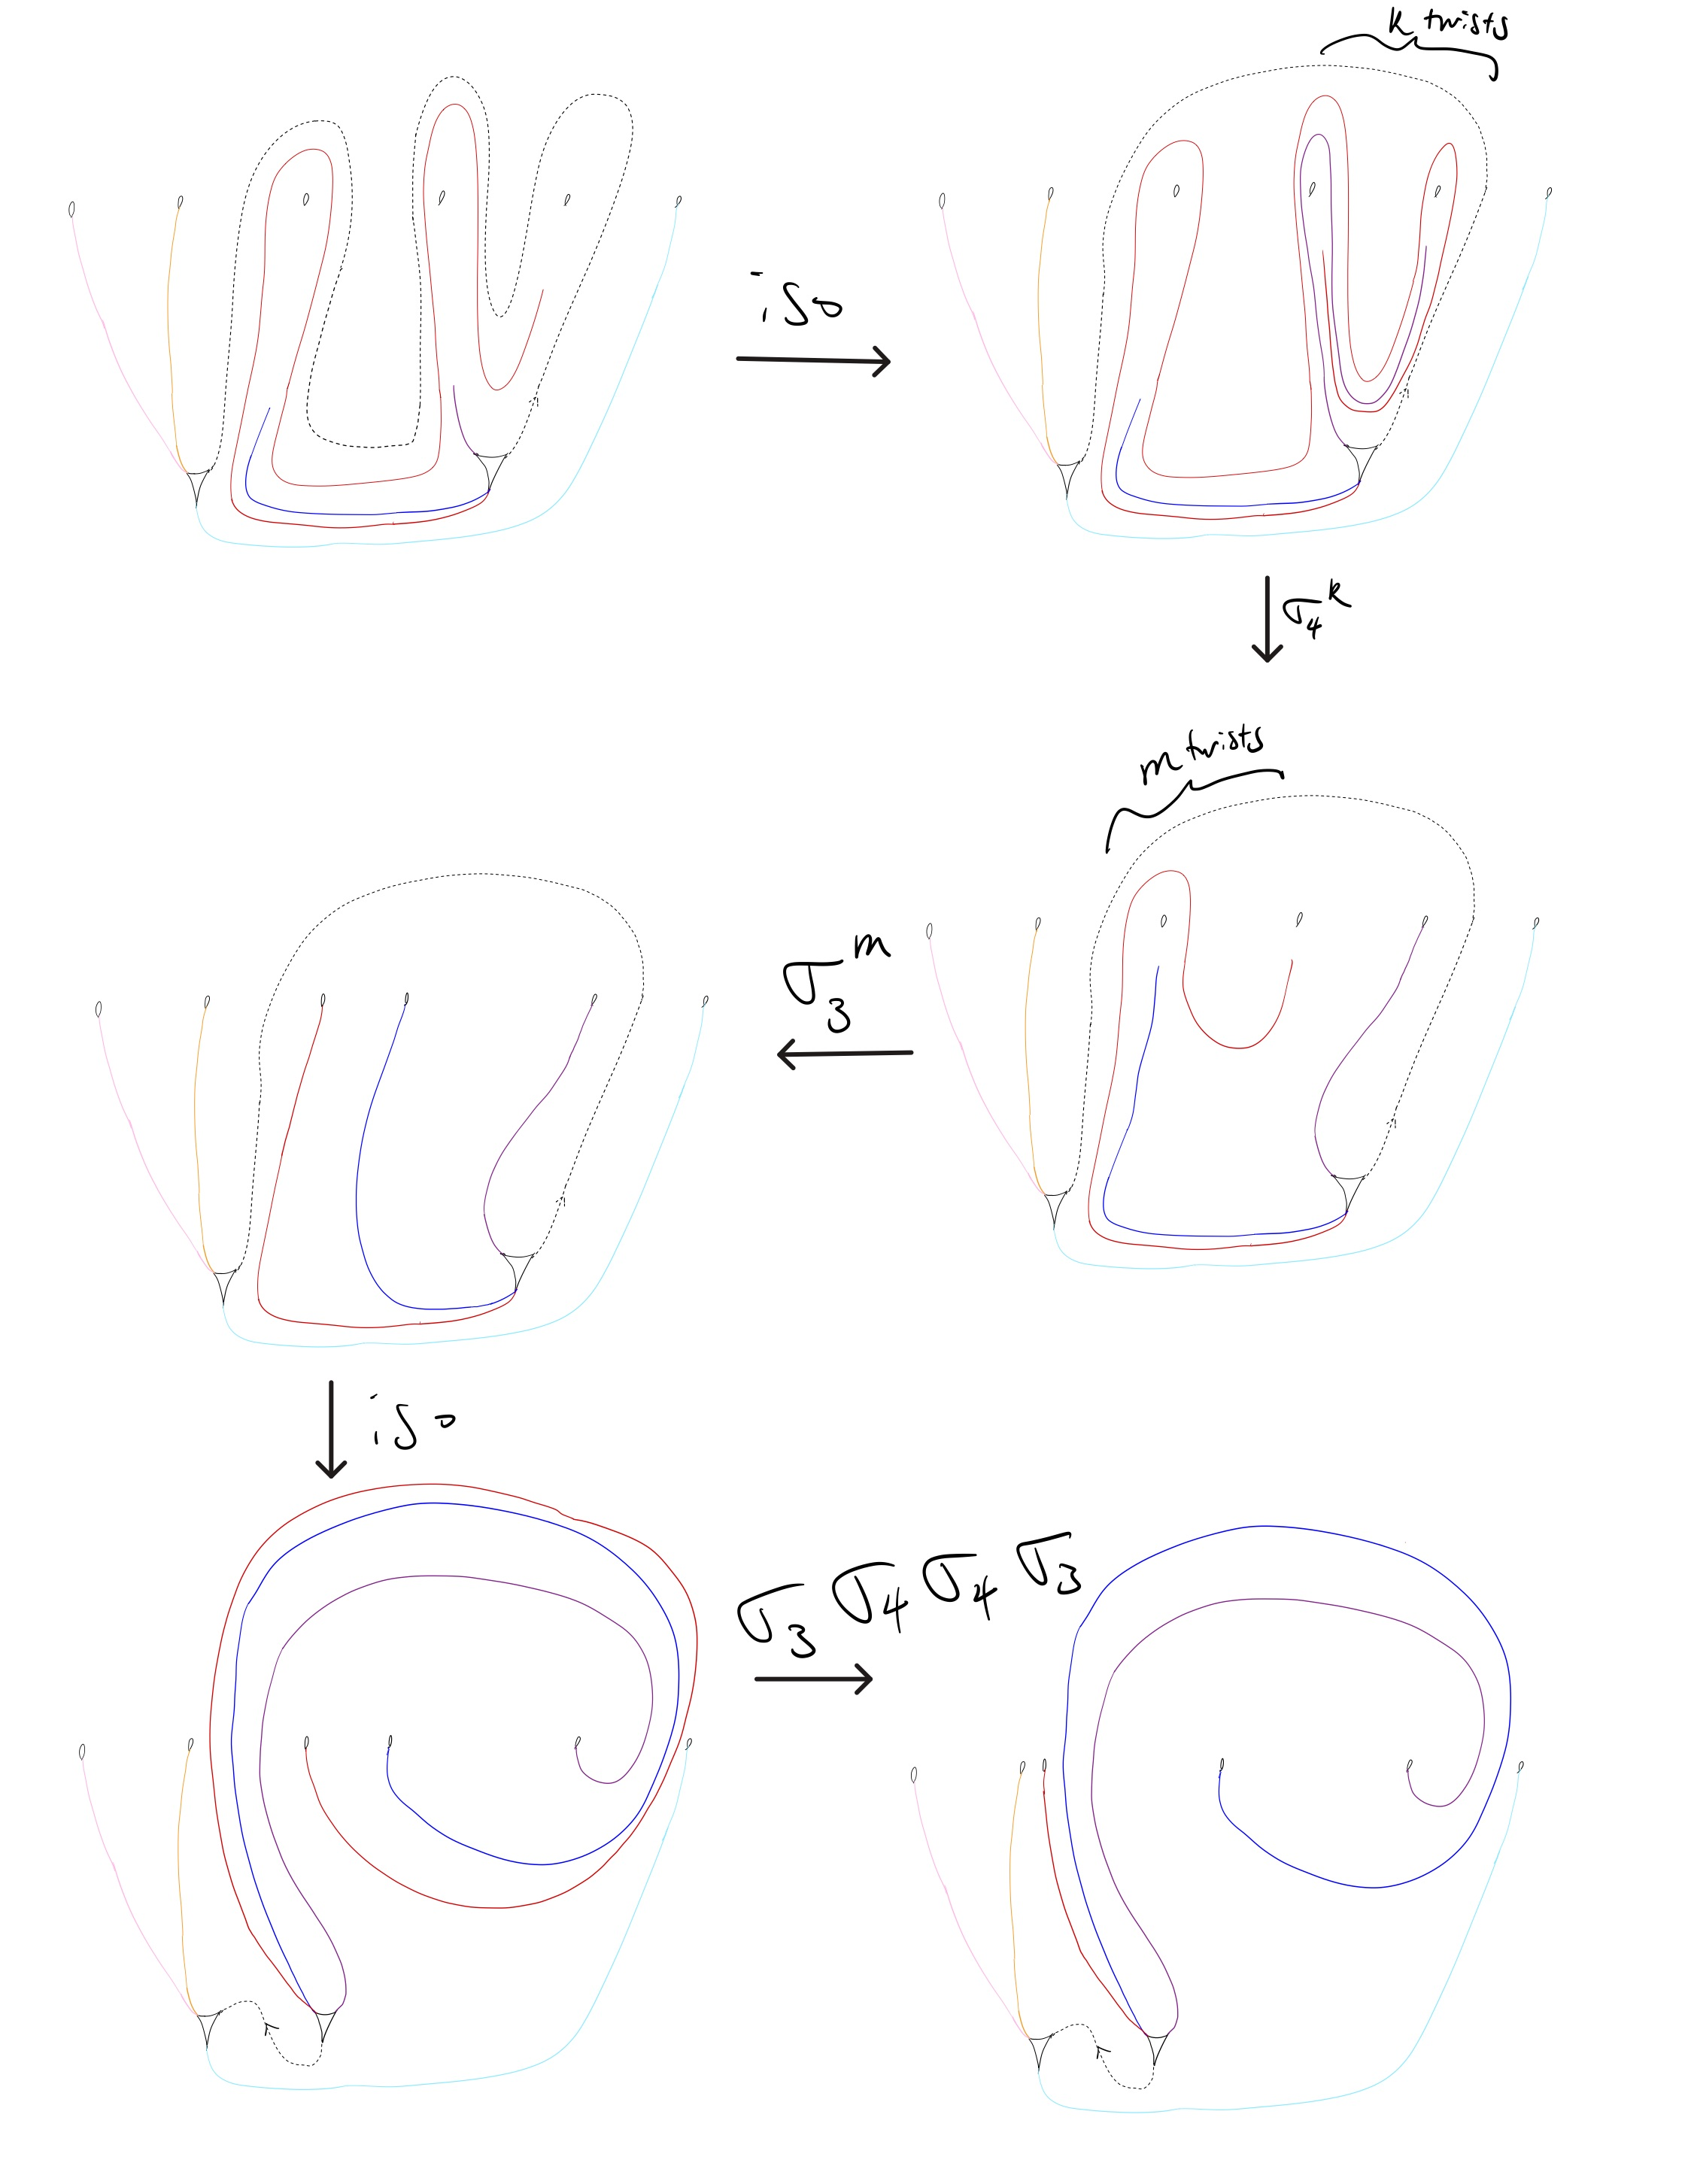
\includegraphics[width=\linewidth, height=0.45\textheight, keepaspectratio]{figures_braid/figures_track_0/Track 0 Braid 8 Briefing-2.jpg}\\
    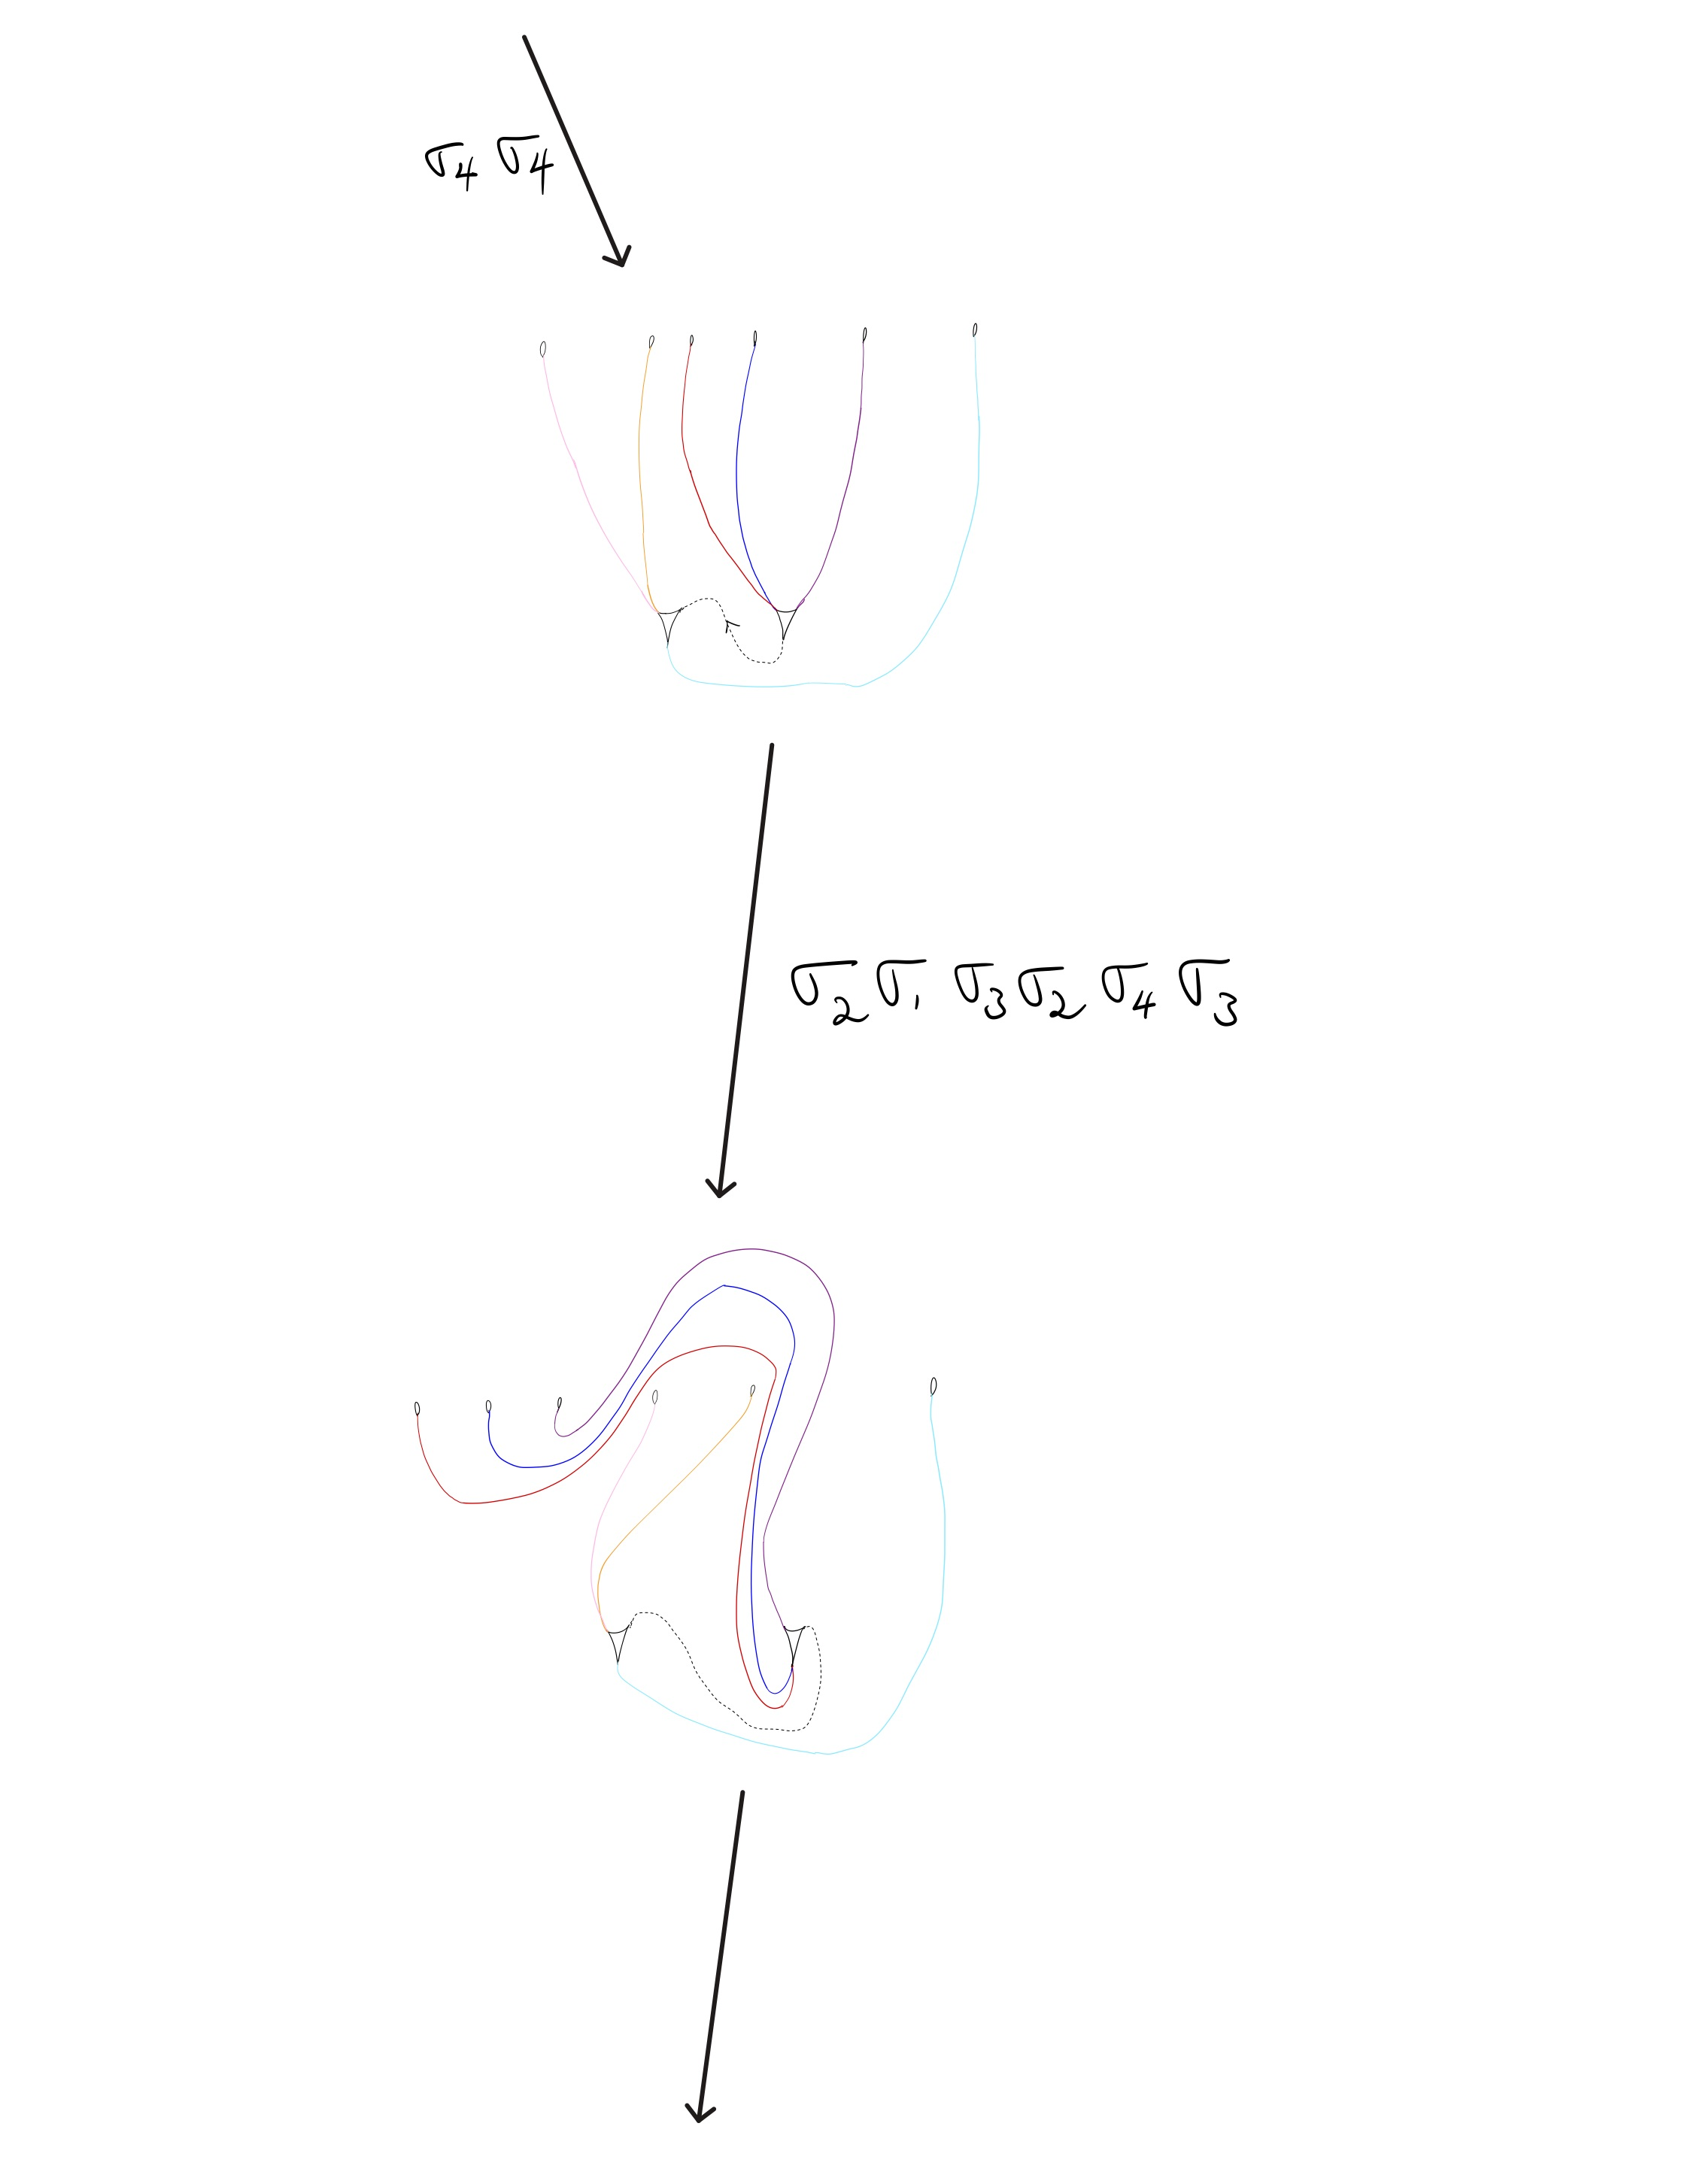
\includegraphics[width=\linewidth, height=0.45\textheight, keepaspectratio]{figures_braid/figures_track_0/Track 0 Braid 8 Briefing-3.jpg}
    \caption{This sequence shows the inverse of the braid $b_8^0$ carries Train Track Candidate Family 8.}
    \label{fig:track0_braid_b0_8}
\end{figure*}

\begin{figure*}[p]
    \ContinuedFloat
    \centering
    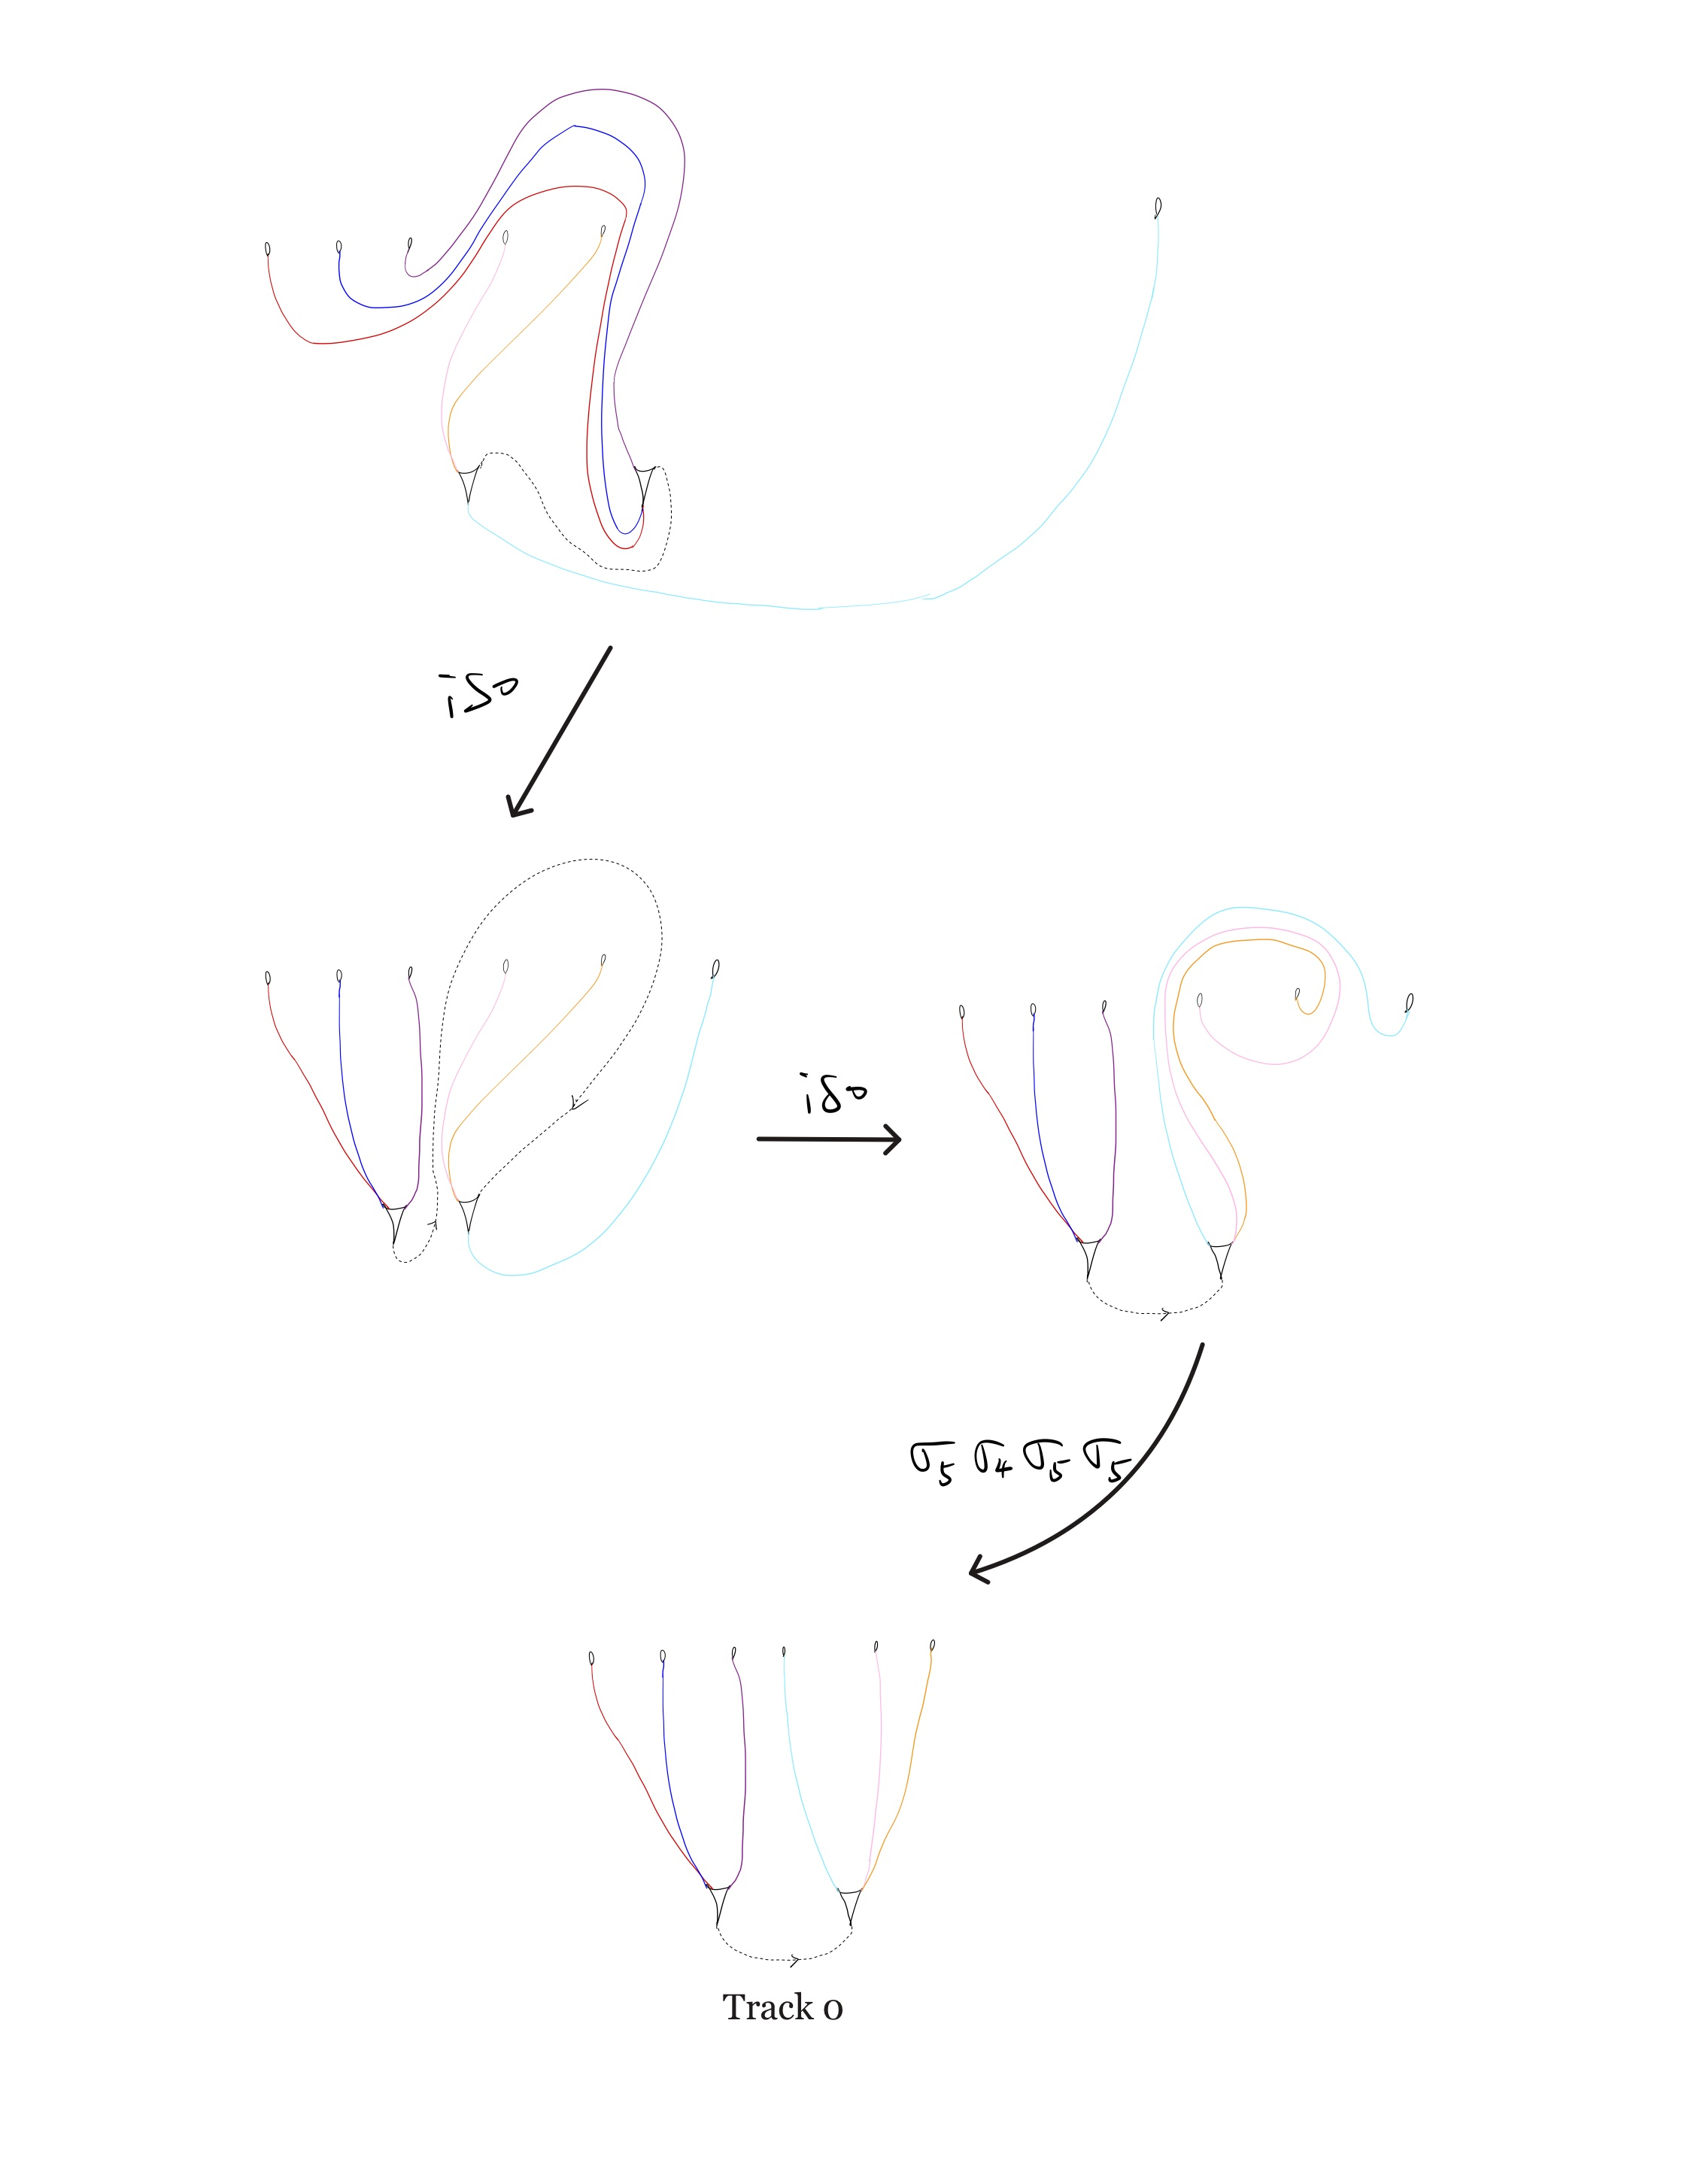
\includegraphics[width=\linewidth, height=0.45\textheight, keepaspectratio]{figures_braid/figures_track_0/Track 0 Braid 8 Briefing-4.jpg}
    \caption[]{This sequence shows the inverse of the braid $b_8^0$ carries Train Track Candidate Family 8 (continued).}
\end{figure*}

\clearpage

\section{Candidate Family 9 (Quail)}\label{sec:track0_quail_1}
Train Track Map Candidate Family 9 of Track 0 is shown in Figure \ref{fig:track0_braid_b0_9_map}. See \ref{Quail} for details.

\begin{figure*}[ht]
    \centering
    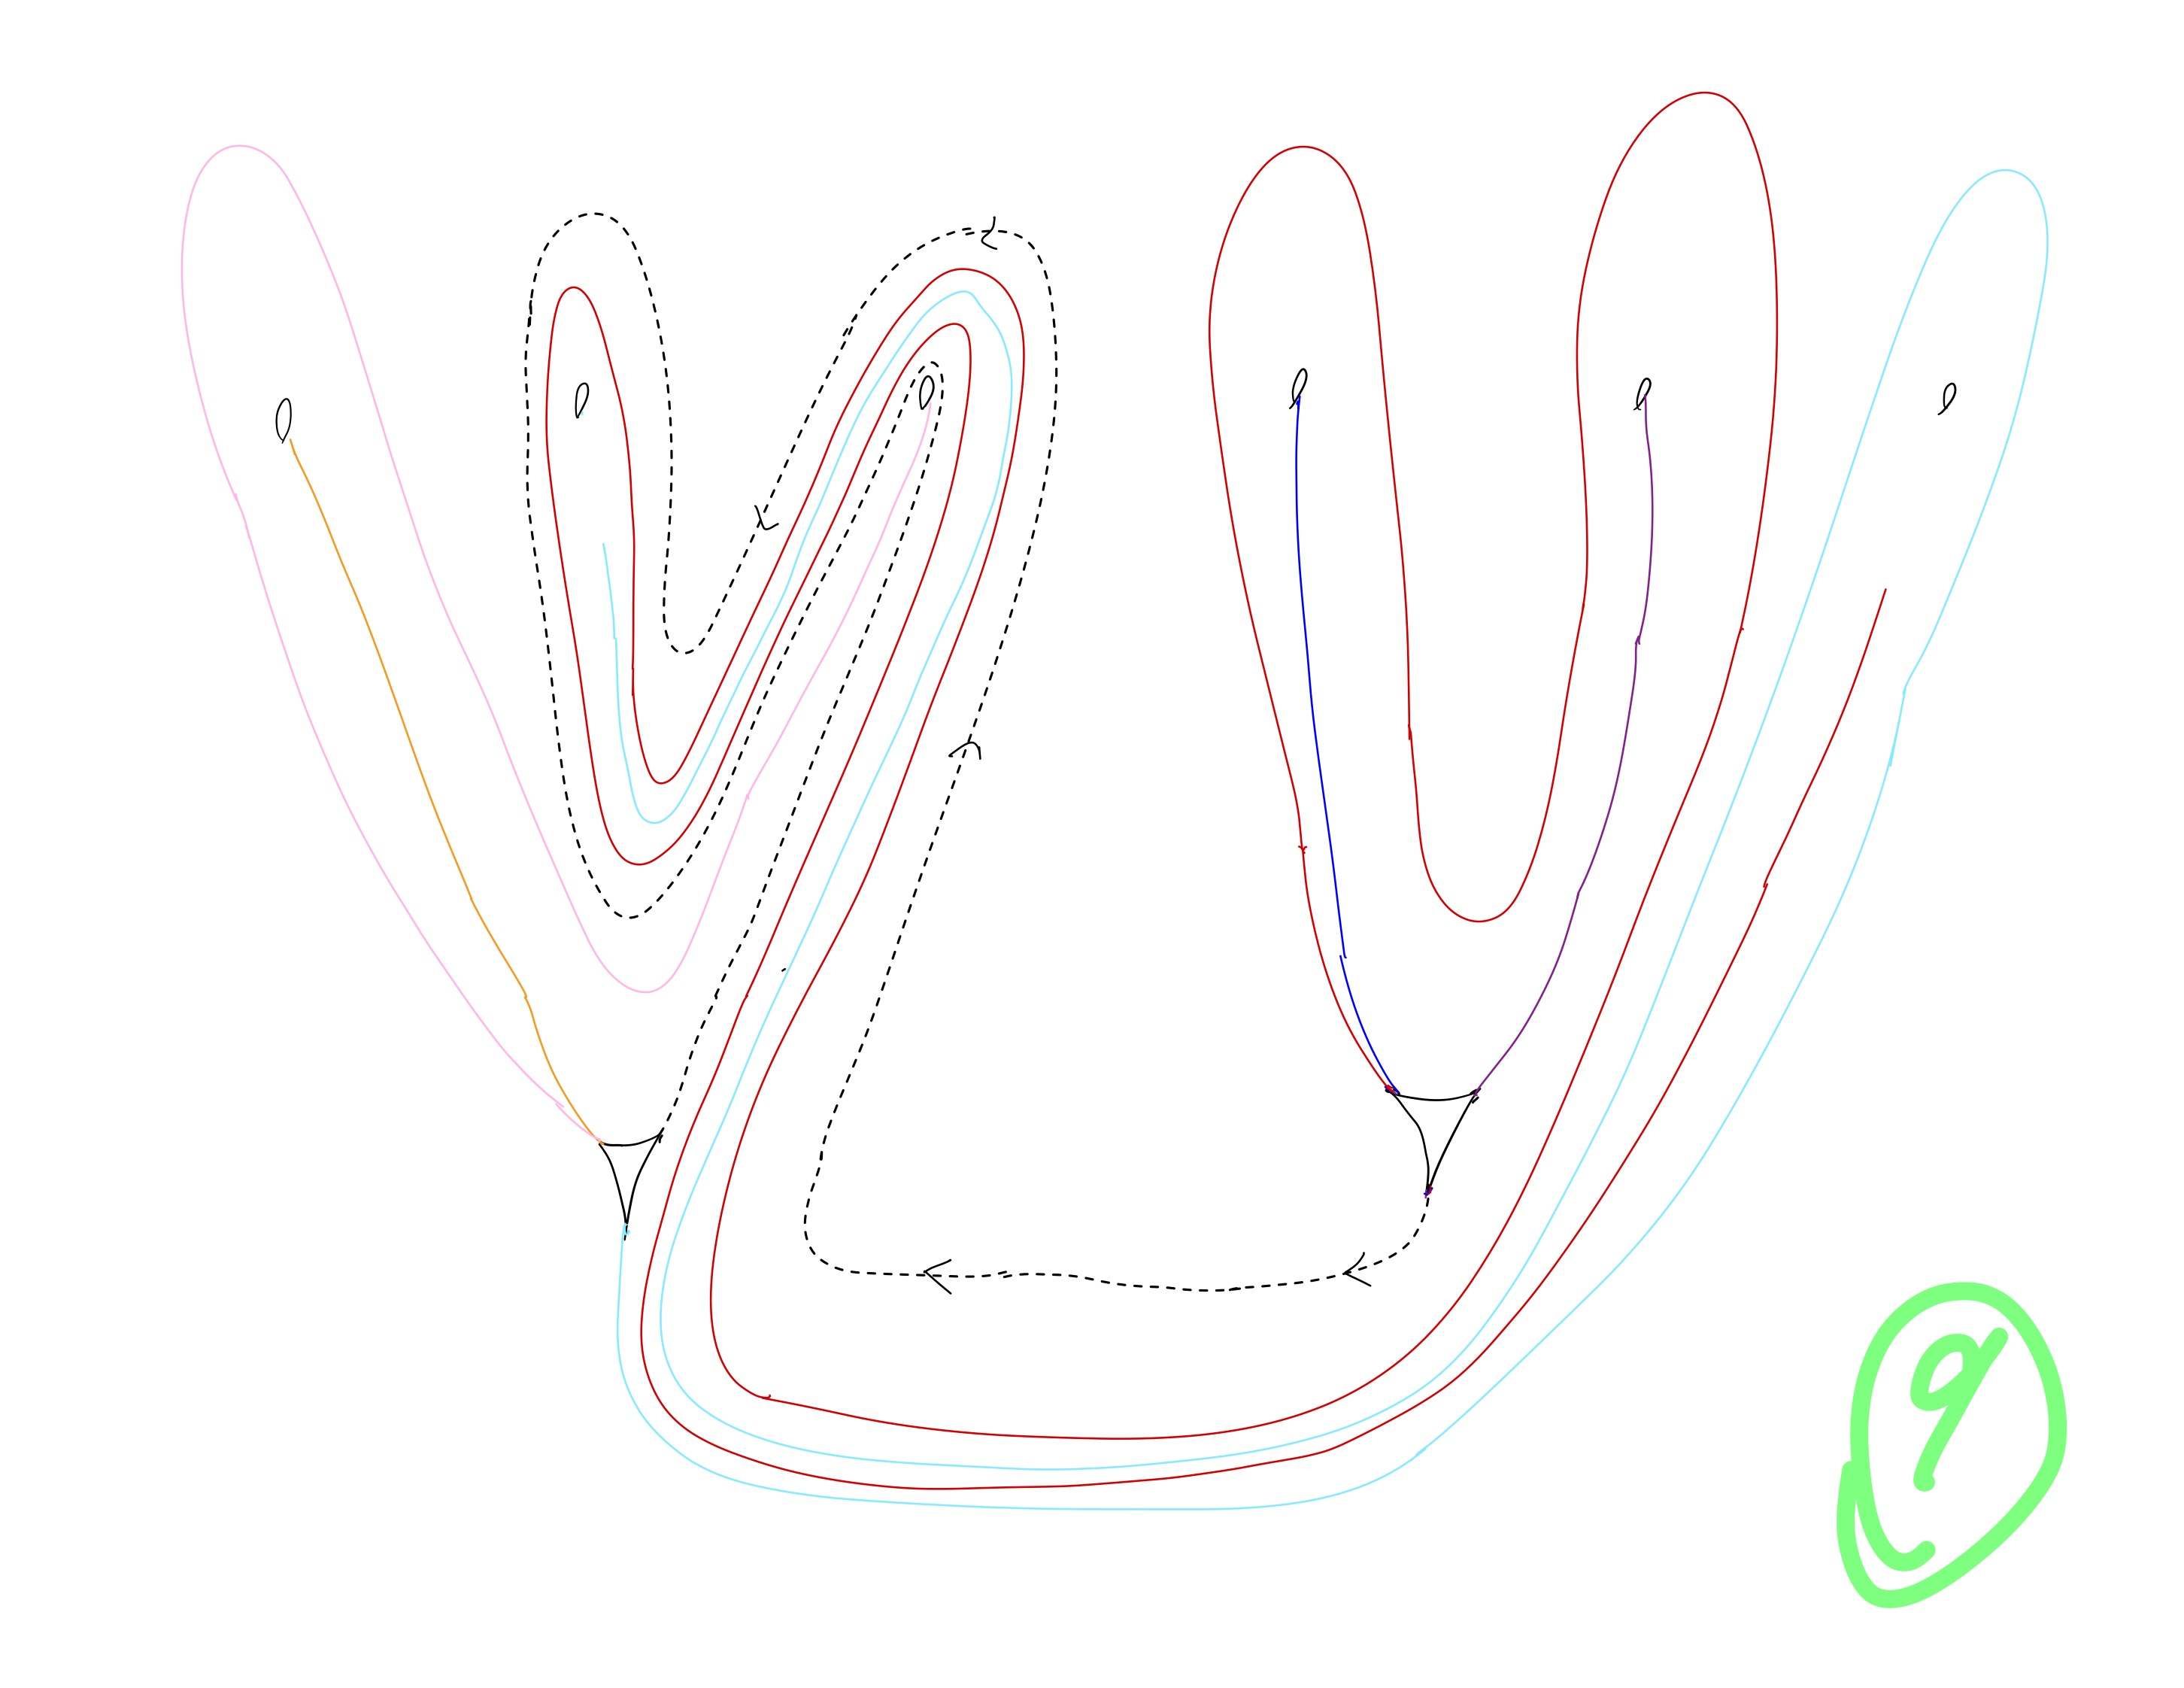
\includegraphics[width=\linewidth, height=0.45\textheight, keepaspectratio]{figures_braid/figures_track_0/Track 0 Braid 9 Quail-1.jpg}
    \caption{Train Track Map Candidate Family 9 of Track 0.}
    \label{fig:track0_braid_b0_9_map}
\end{figure*}

The inverse of the following braid carries this family of train track maps:
\[
b_9^0 = \sigma_{2}^{-1} \sigma_{1} \sigma_{3} \sigma_{4} \sigma_{5}^{-k} \sigma_{4} \sigma_{3} \sigma_{2} \sigma_{1} \sigma_{3} \sigma_{2} \sigma_{4} \sigma_{3} \sigma_{5} \sigma_{4} \sigma_{5} \sigma_{5}
\]
where $k \geq 1$ ($k \in \mathbb{Z}$) is the twisting parameter. This is shown in Figure \ref{fig:track0_braid_b0_9}.

\begin{figure*}[p]
    \centering
    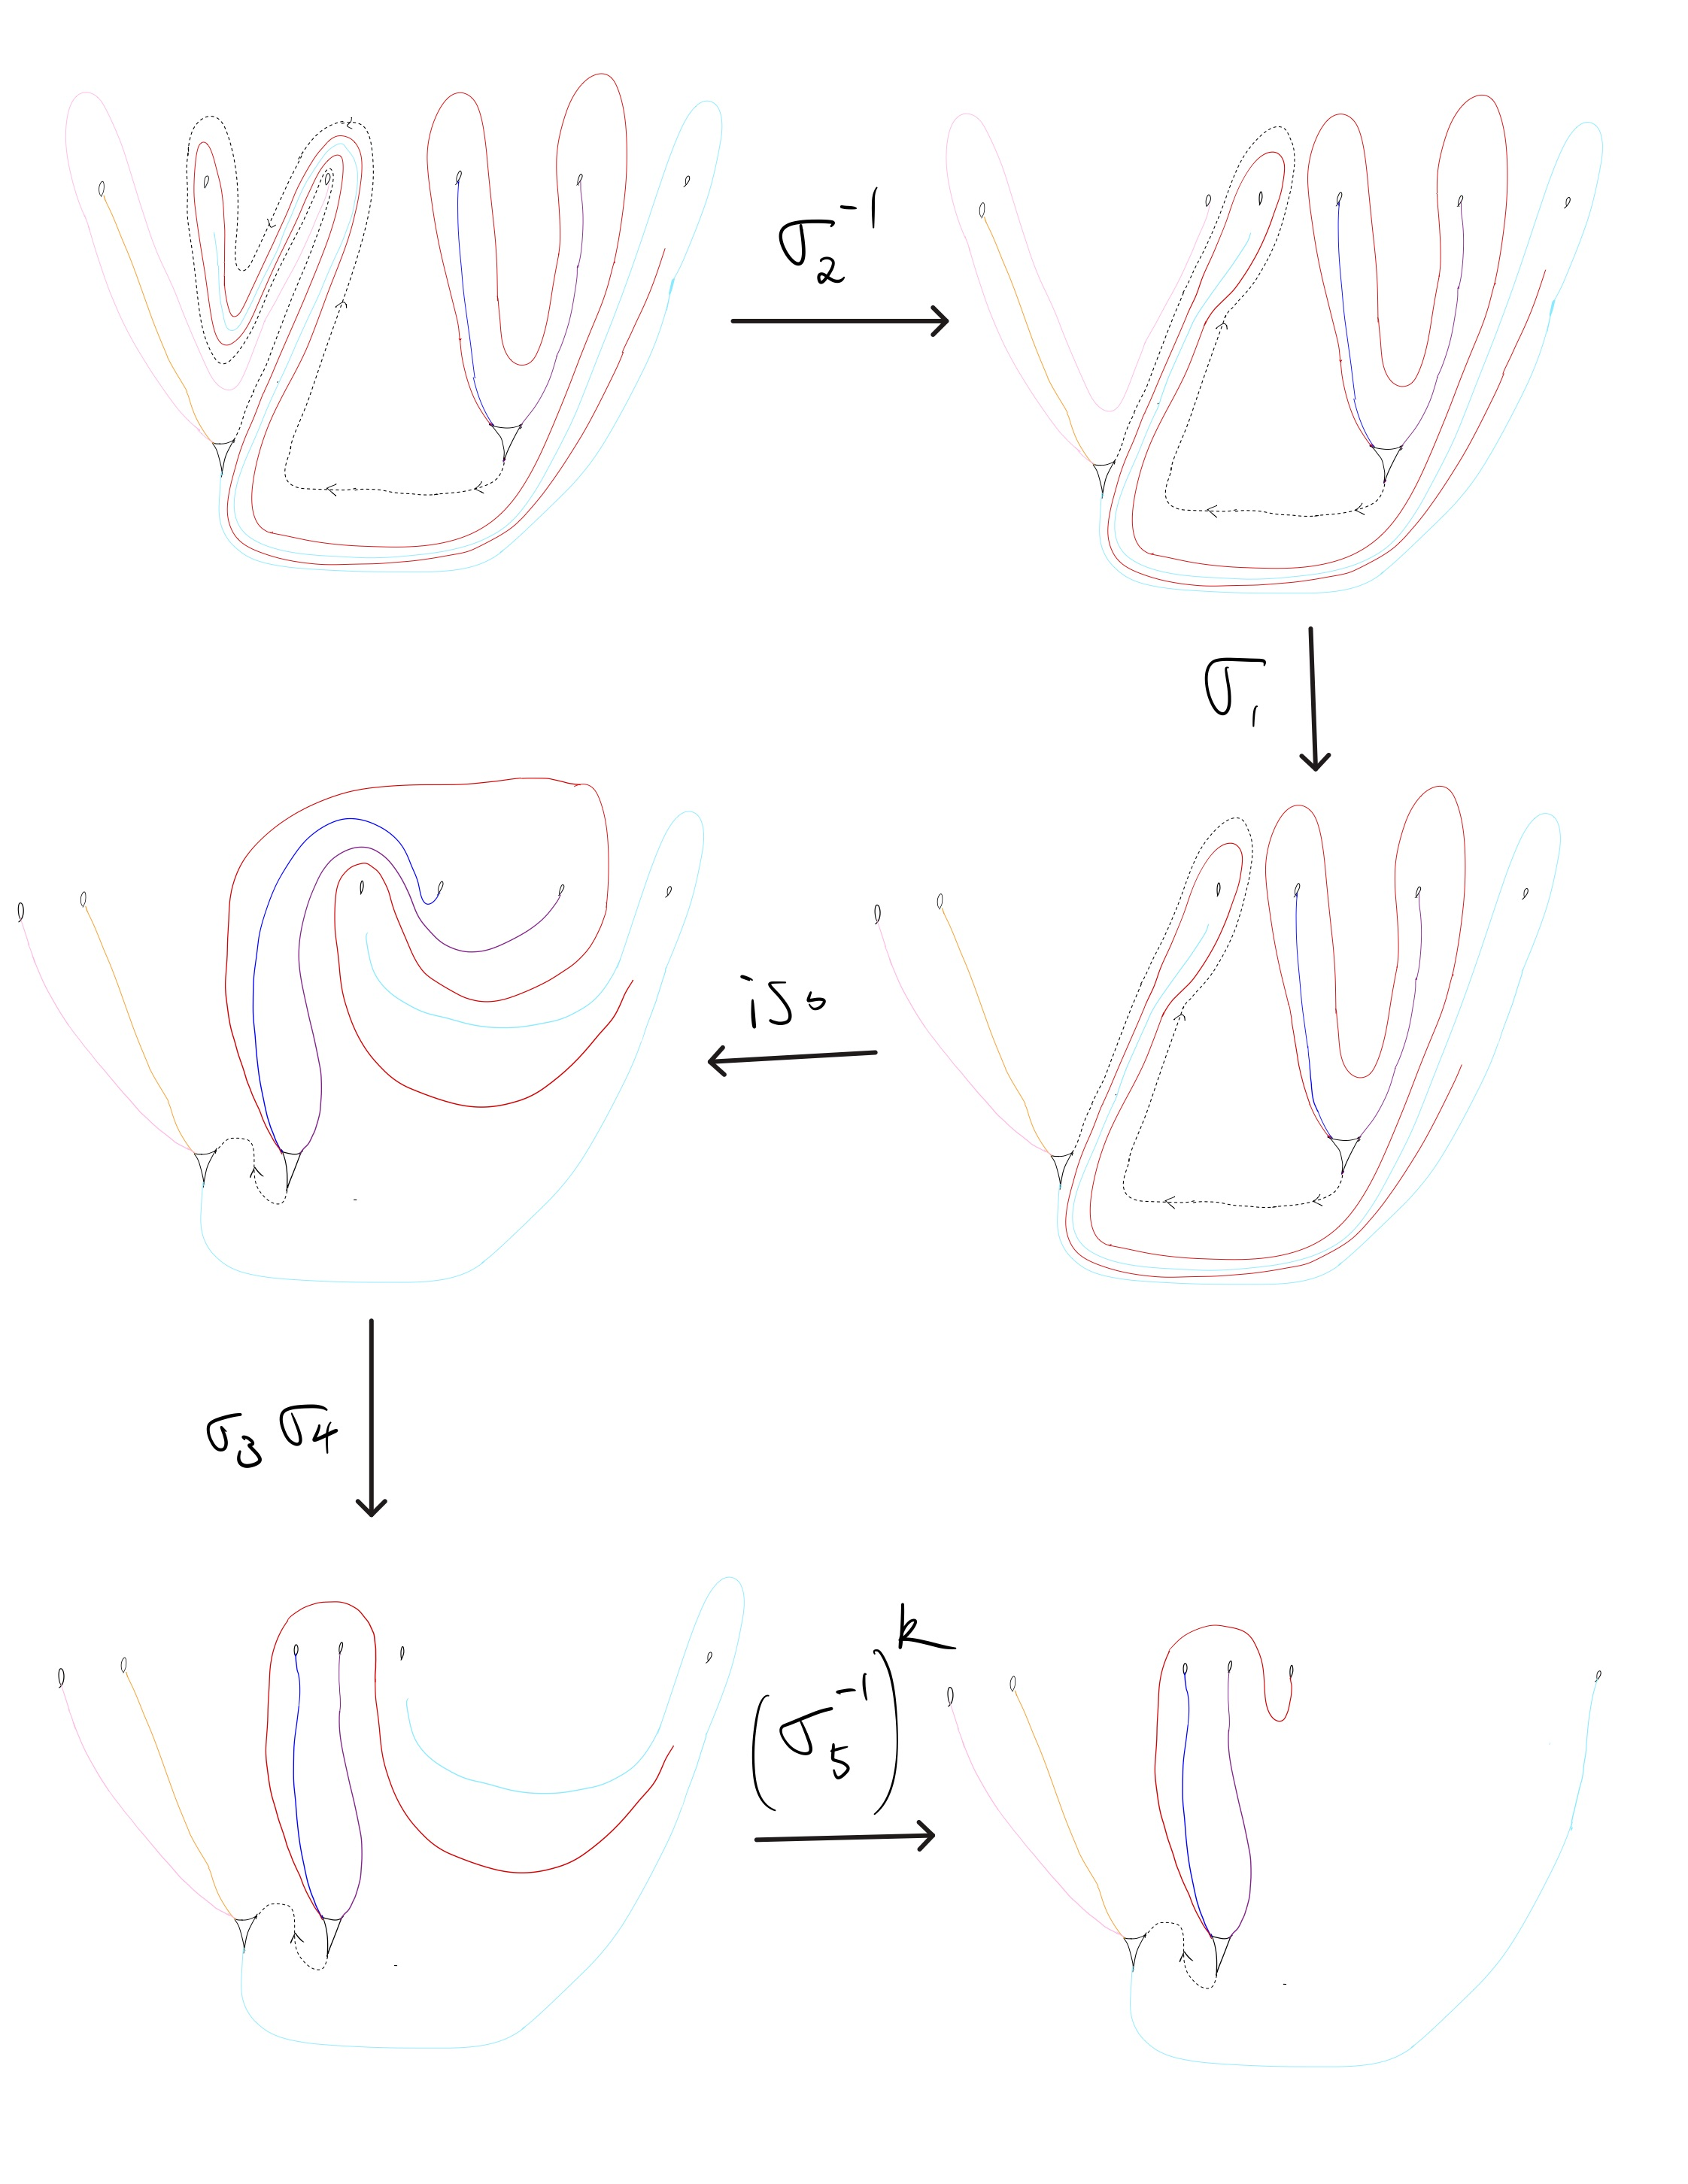
\includegraphics[width=\linewidth, height=0.45\textheight, keepaspectratio]{figures_braid/figures_track_0/Track 0 Braid 9 Quail-2.jpg}\\
    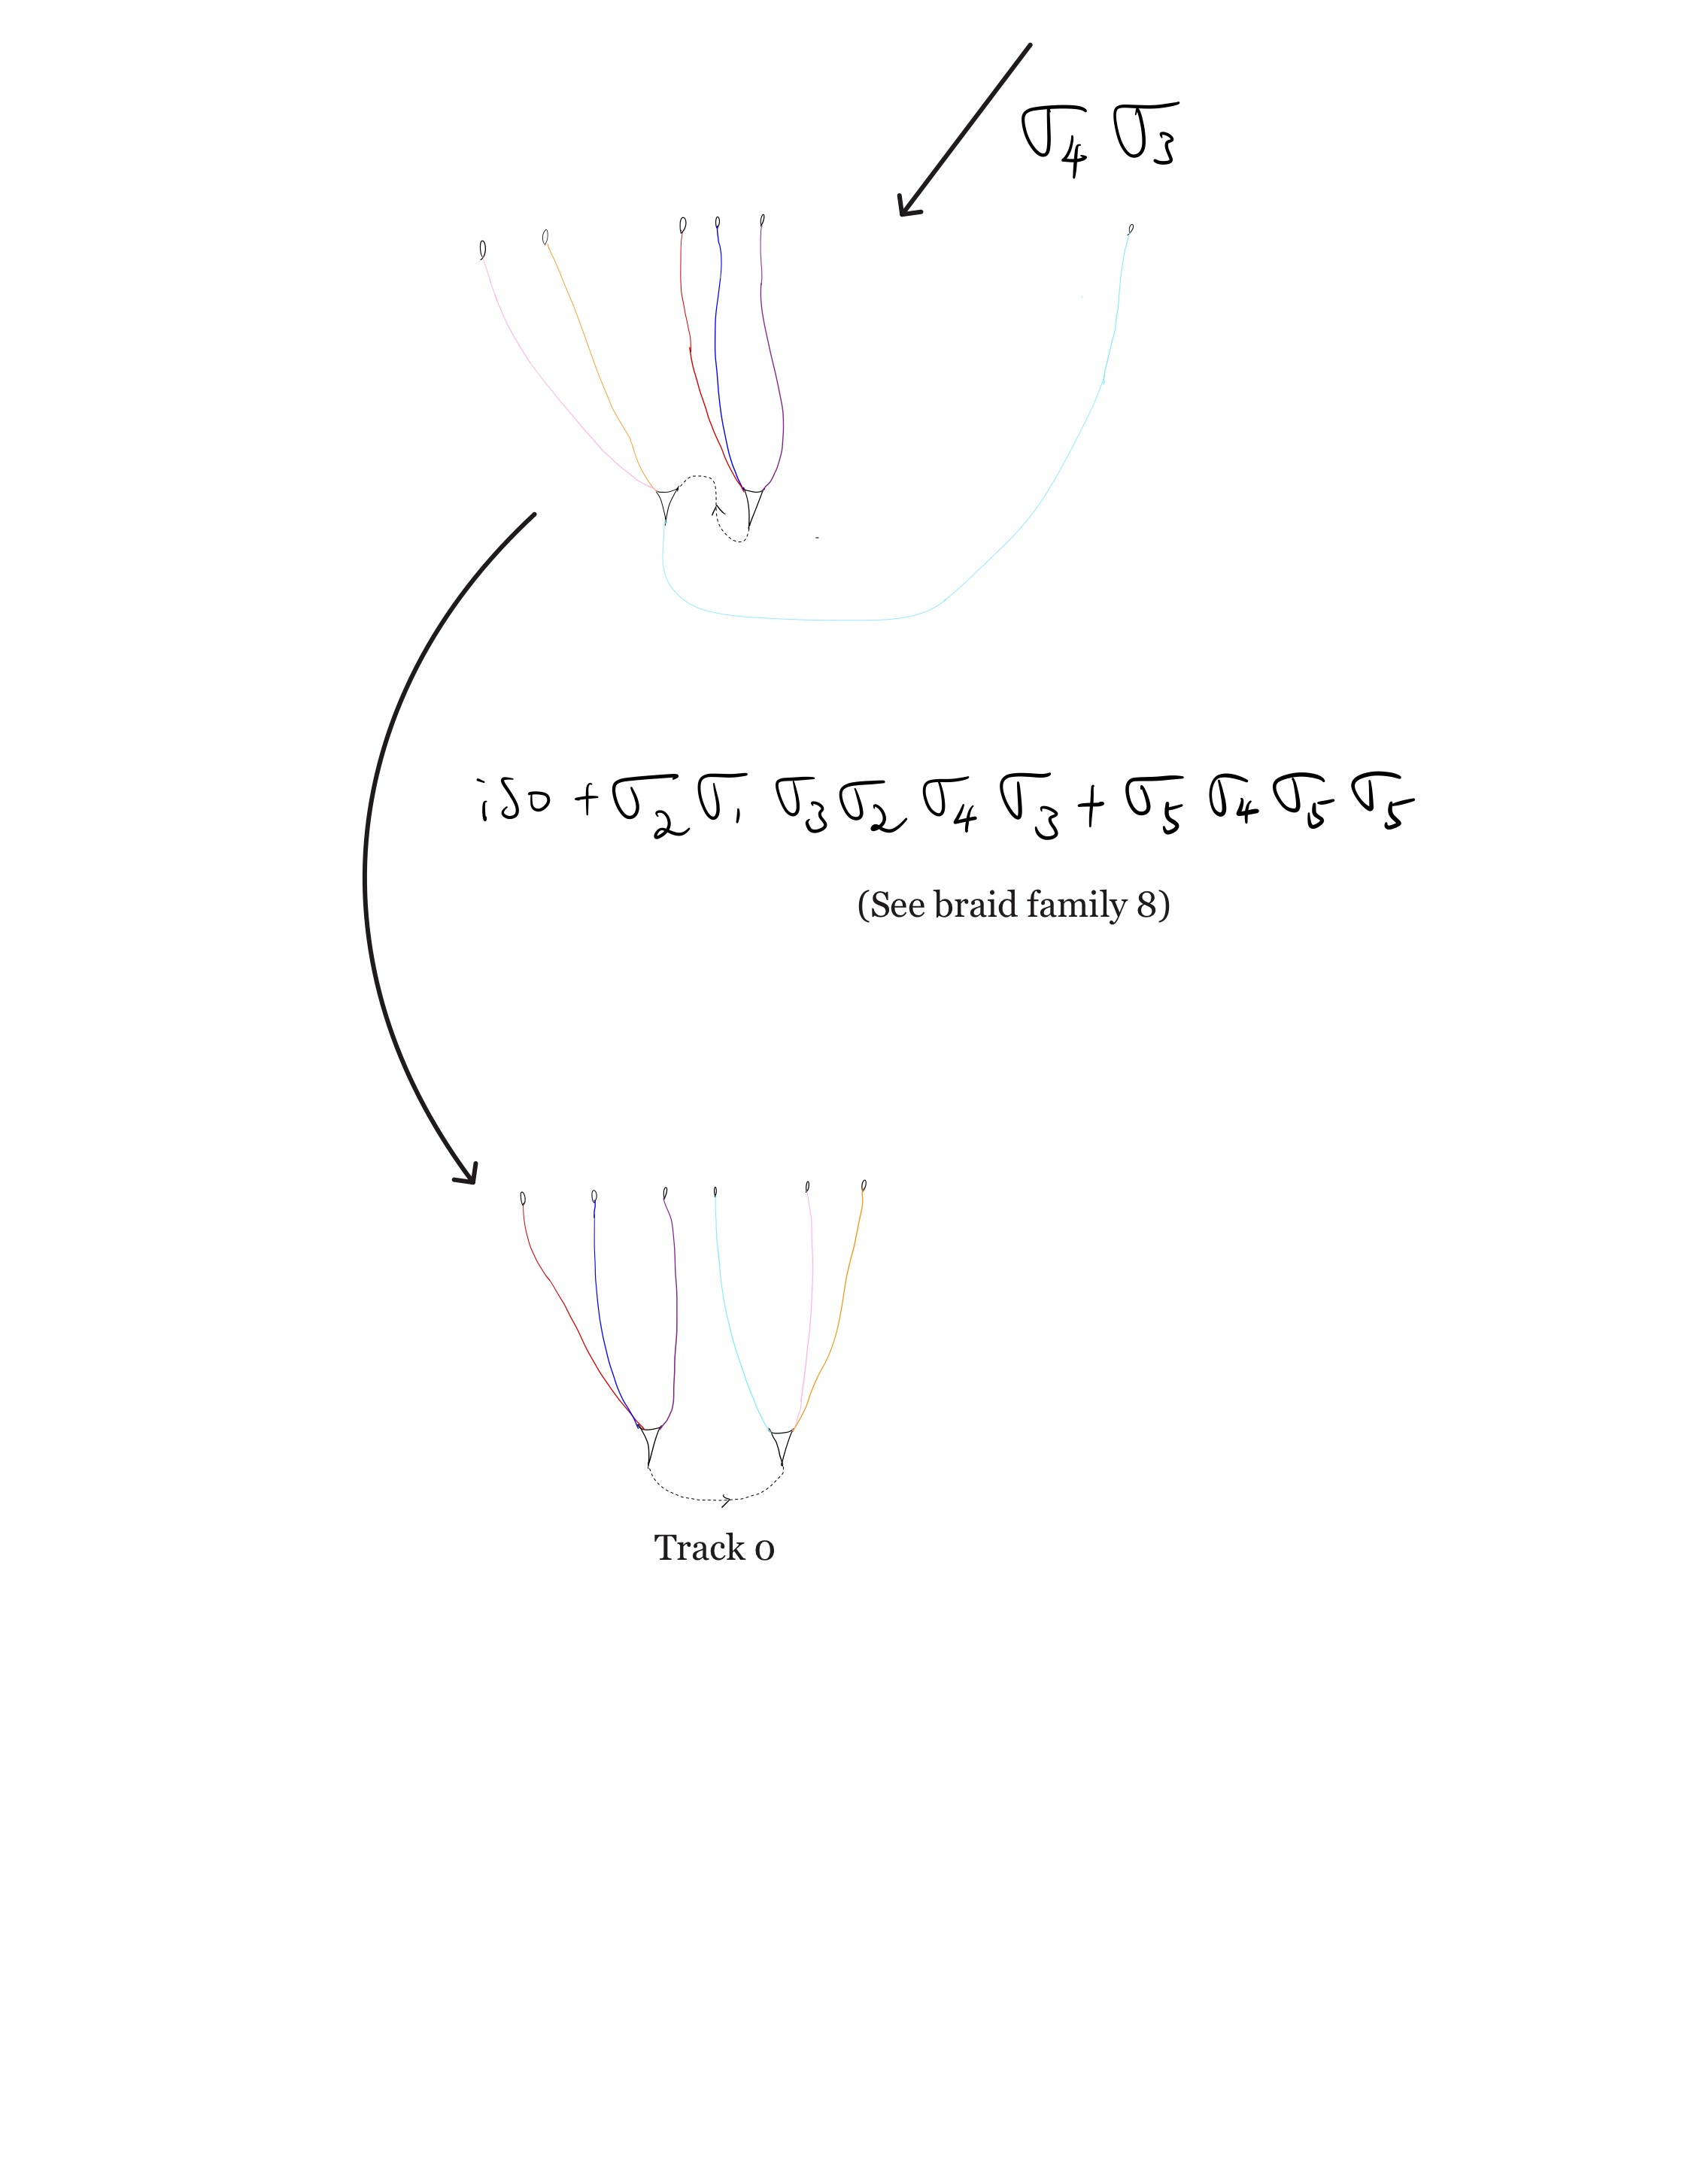
\includegraphics[width=\linewidth, height=0.45\textheight, keepaspectratio]{figures_braid/figures_track_0/Track 0 Braid 9 Quail-3.jpg}
    \caption{This sequence shows the inverse of the braid $b_9^0$ carries Train Track Candidate Family 9.}
    \label{fig:track0_braid_b0_9}
\end{figure*}

\clearpage

\section{Candidate Family 10 (Quail)}\label{sec:track0_quail_2}
Train Track Map Candidate Family 10 of Track 0 is shown in Figure \ref{fig:track0_braid_b0_10_map}. See \ref{Quail} for details.

\begin{figure*}[ht]
    \centering
    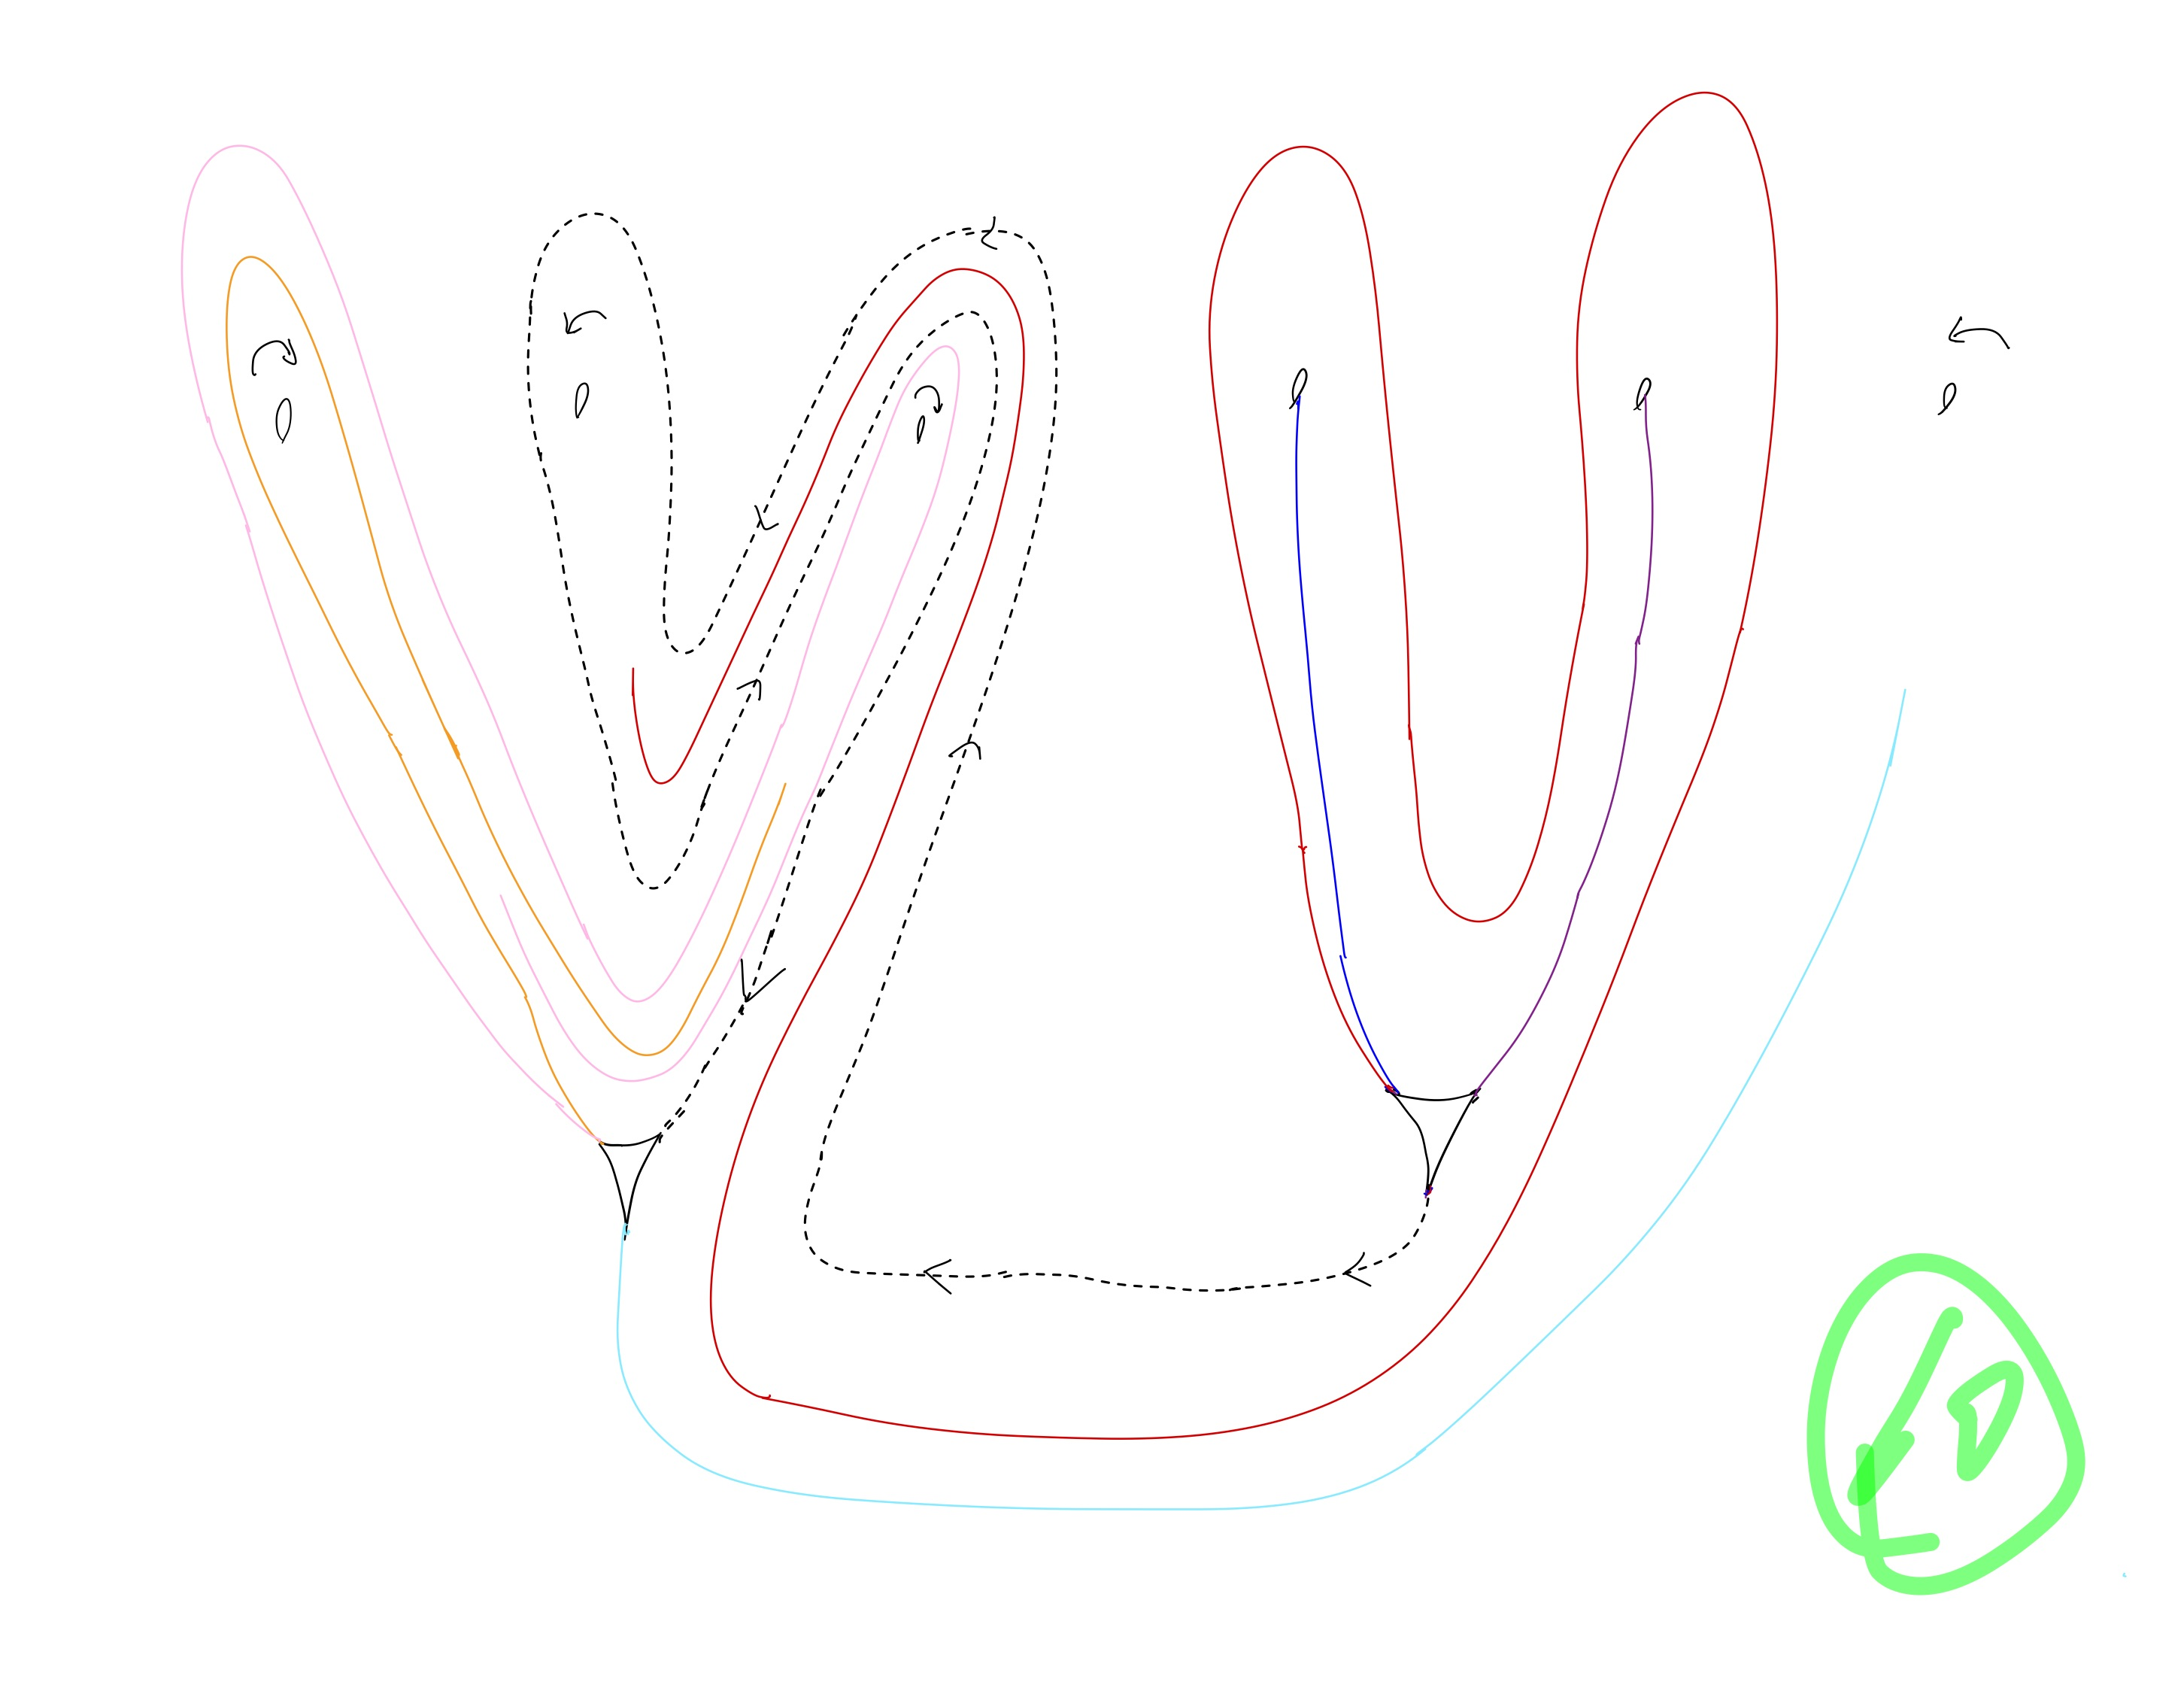
\includegraphics[width=\linewidth, height=0.45\textheight, keepaspectratio]{figures_braid/figures_track_0/Track 0 Braid 10 Quail-1.jpg}
    \caption{Train Track Map Candidate Family 10 of Track 0.}
    \label{fig:track0_braid_b0_10_map}
\end{figure*}

The inverse of the following braid carries this family of train track maps:
\[
b_{10}^0 = \sigma_{2}^{-j} \sigma_{1}^m \sigma_{3} \sigma_{4} \sigma_{5}^{-k} \sigma_{4} \sigma_{3} \sigma_{2} \sigma_{1} \sigma_{3} \sigma_{2} \sigma_{4} \sigma_{3} \sigma_{5} \sigma_{4} \sigma_{5} \sigma_{5}
\]
where $j, m, k \geq 1$ ($j, m, k \in \mathbb{Z}$) are the twisting parameters. This is shown in Figure \ref{fig:track0_braid_b0_10}.

\begin{figure*}[p]
    \centering
    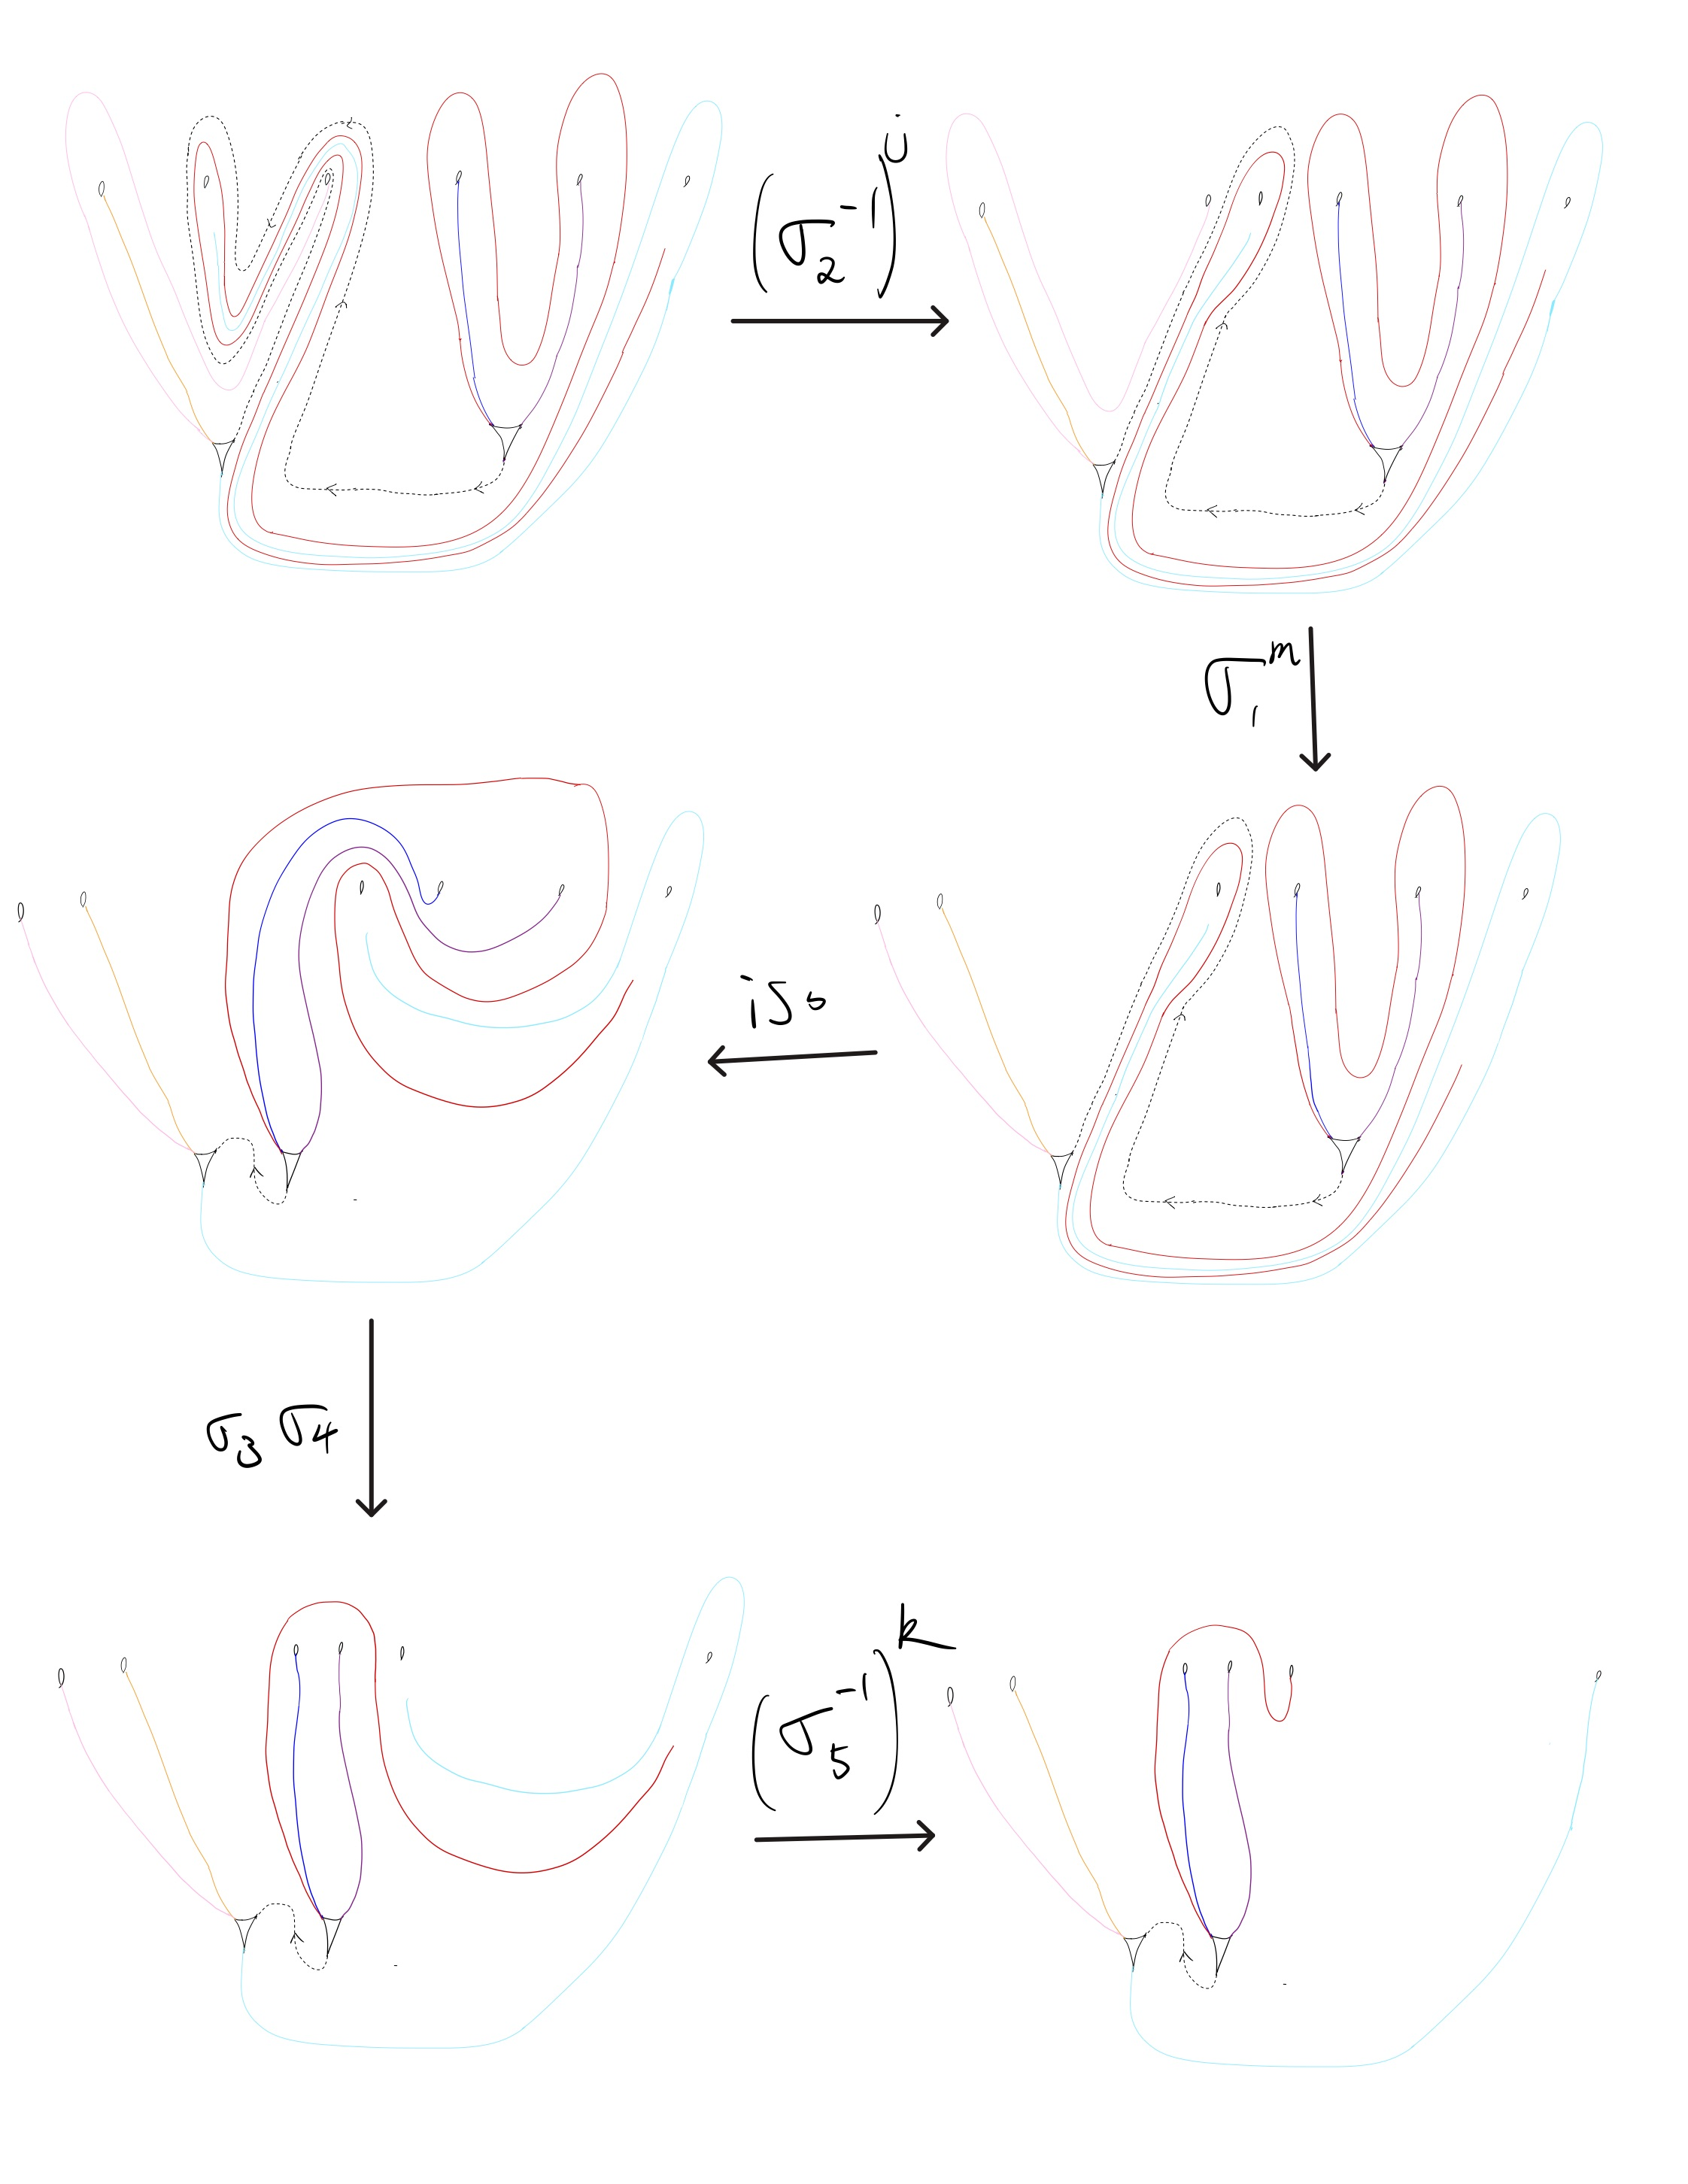
\includegraphics[width=\linewidth, height=0.45\textheight, keepaspectratio]{figures_braid/figures_track_0/Track 0 Braid 10 Quail-2.jpg}\\
    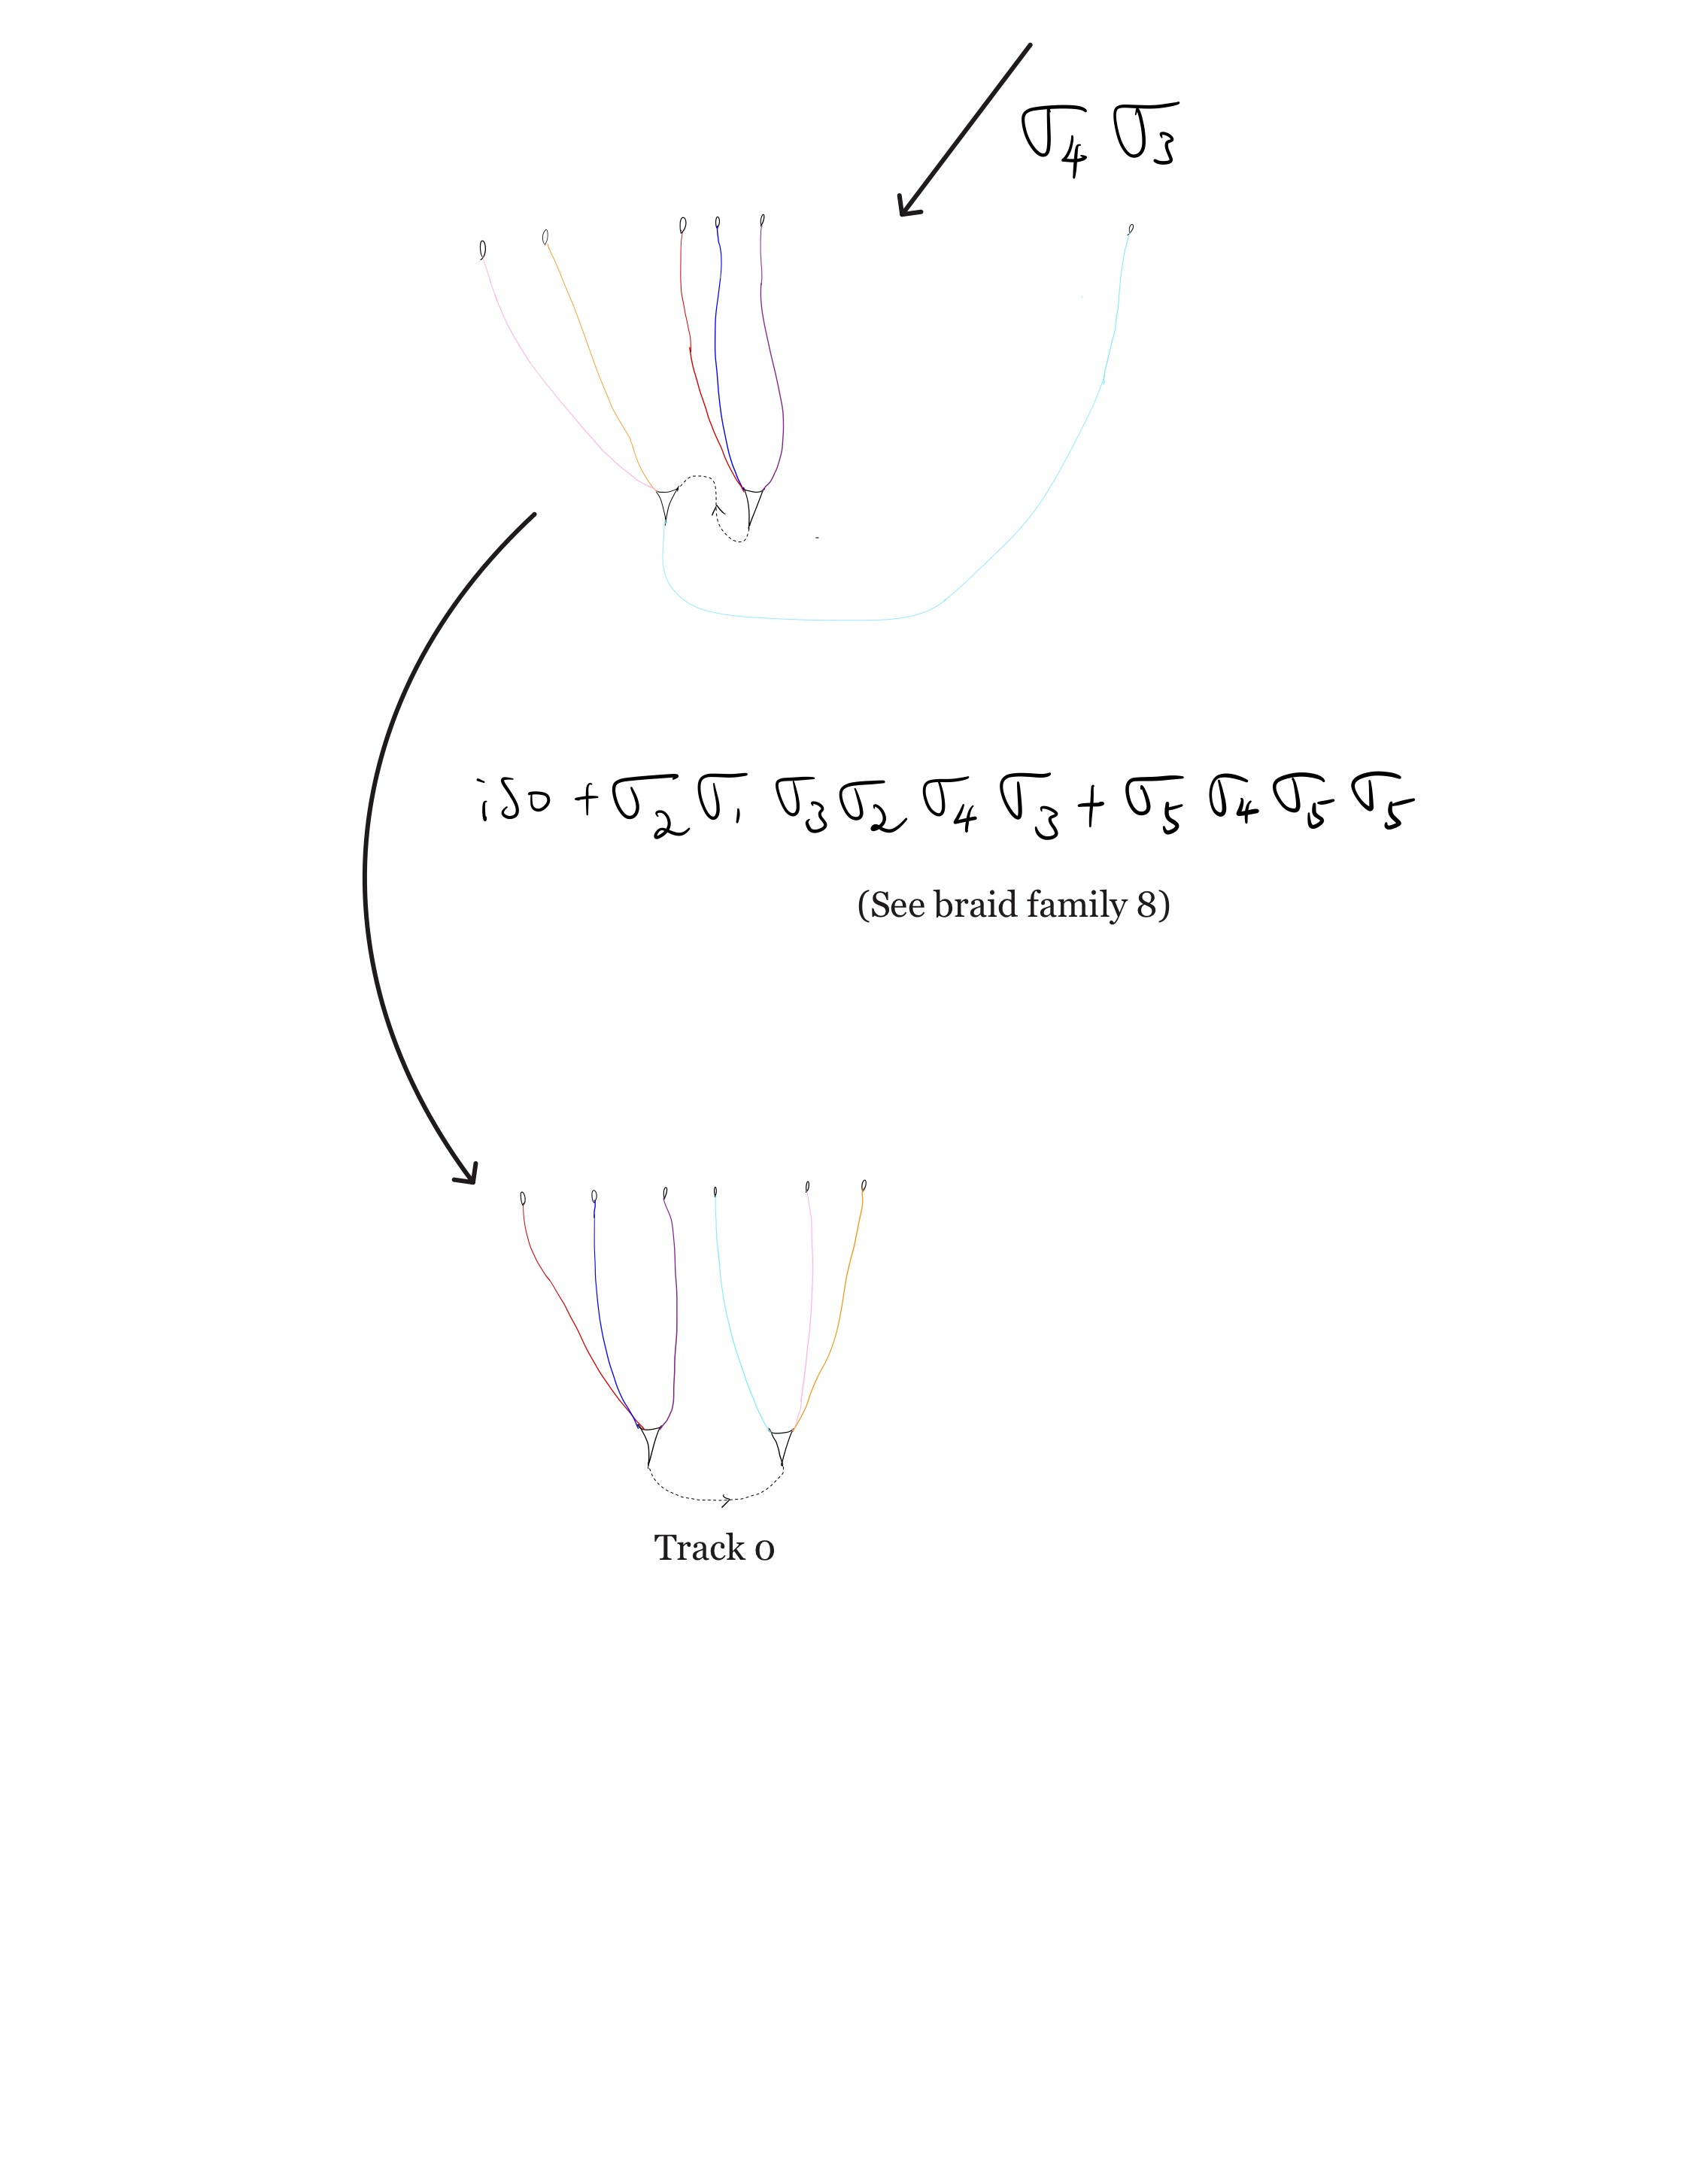
\includegraphics[width=\linewidth, height=0.45\textheight, keepaspectratio]{figures_braid/figures_track_0/Track 0 Braid 10 Quail-3.jpg}
    \caption{This sequence shows the inverse of the braid $b_{10}^0$ carries Train Track Candidate Family 10.}
    \label{fig:track0_braid_b0_10}
\end{figure*}

\clearpage

\section{Candidate Family 11 (Jubilant)}\label{sec:track0_jubilant_1}
Train Track Map Candidate Family 11 of Track 0 is shown in Figure \ref{fig:track0_braid_b0_11_map}. See \ref{Jubilant} for details.

\begin{figure*}[ht]
    \centering
    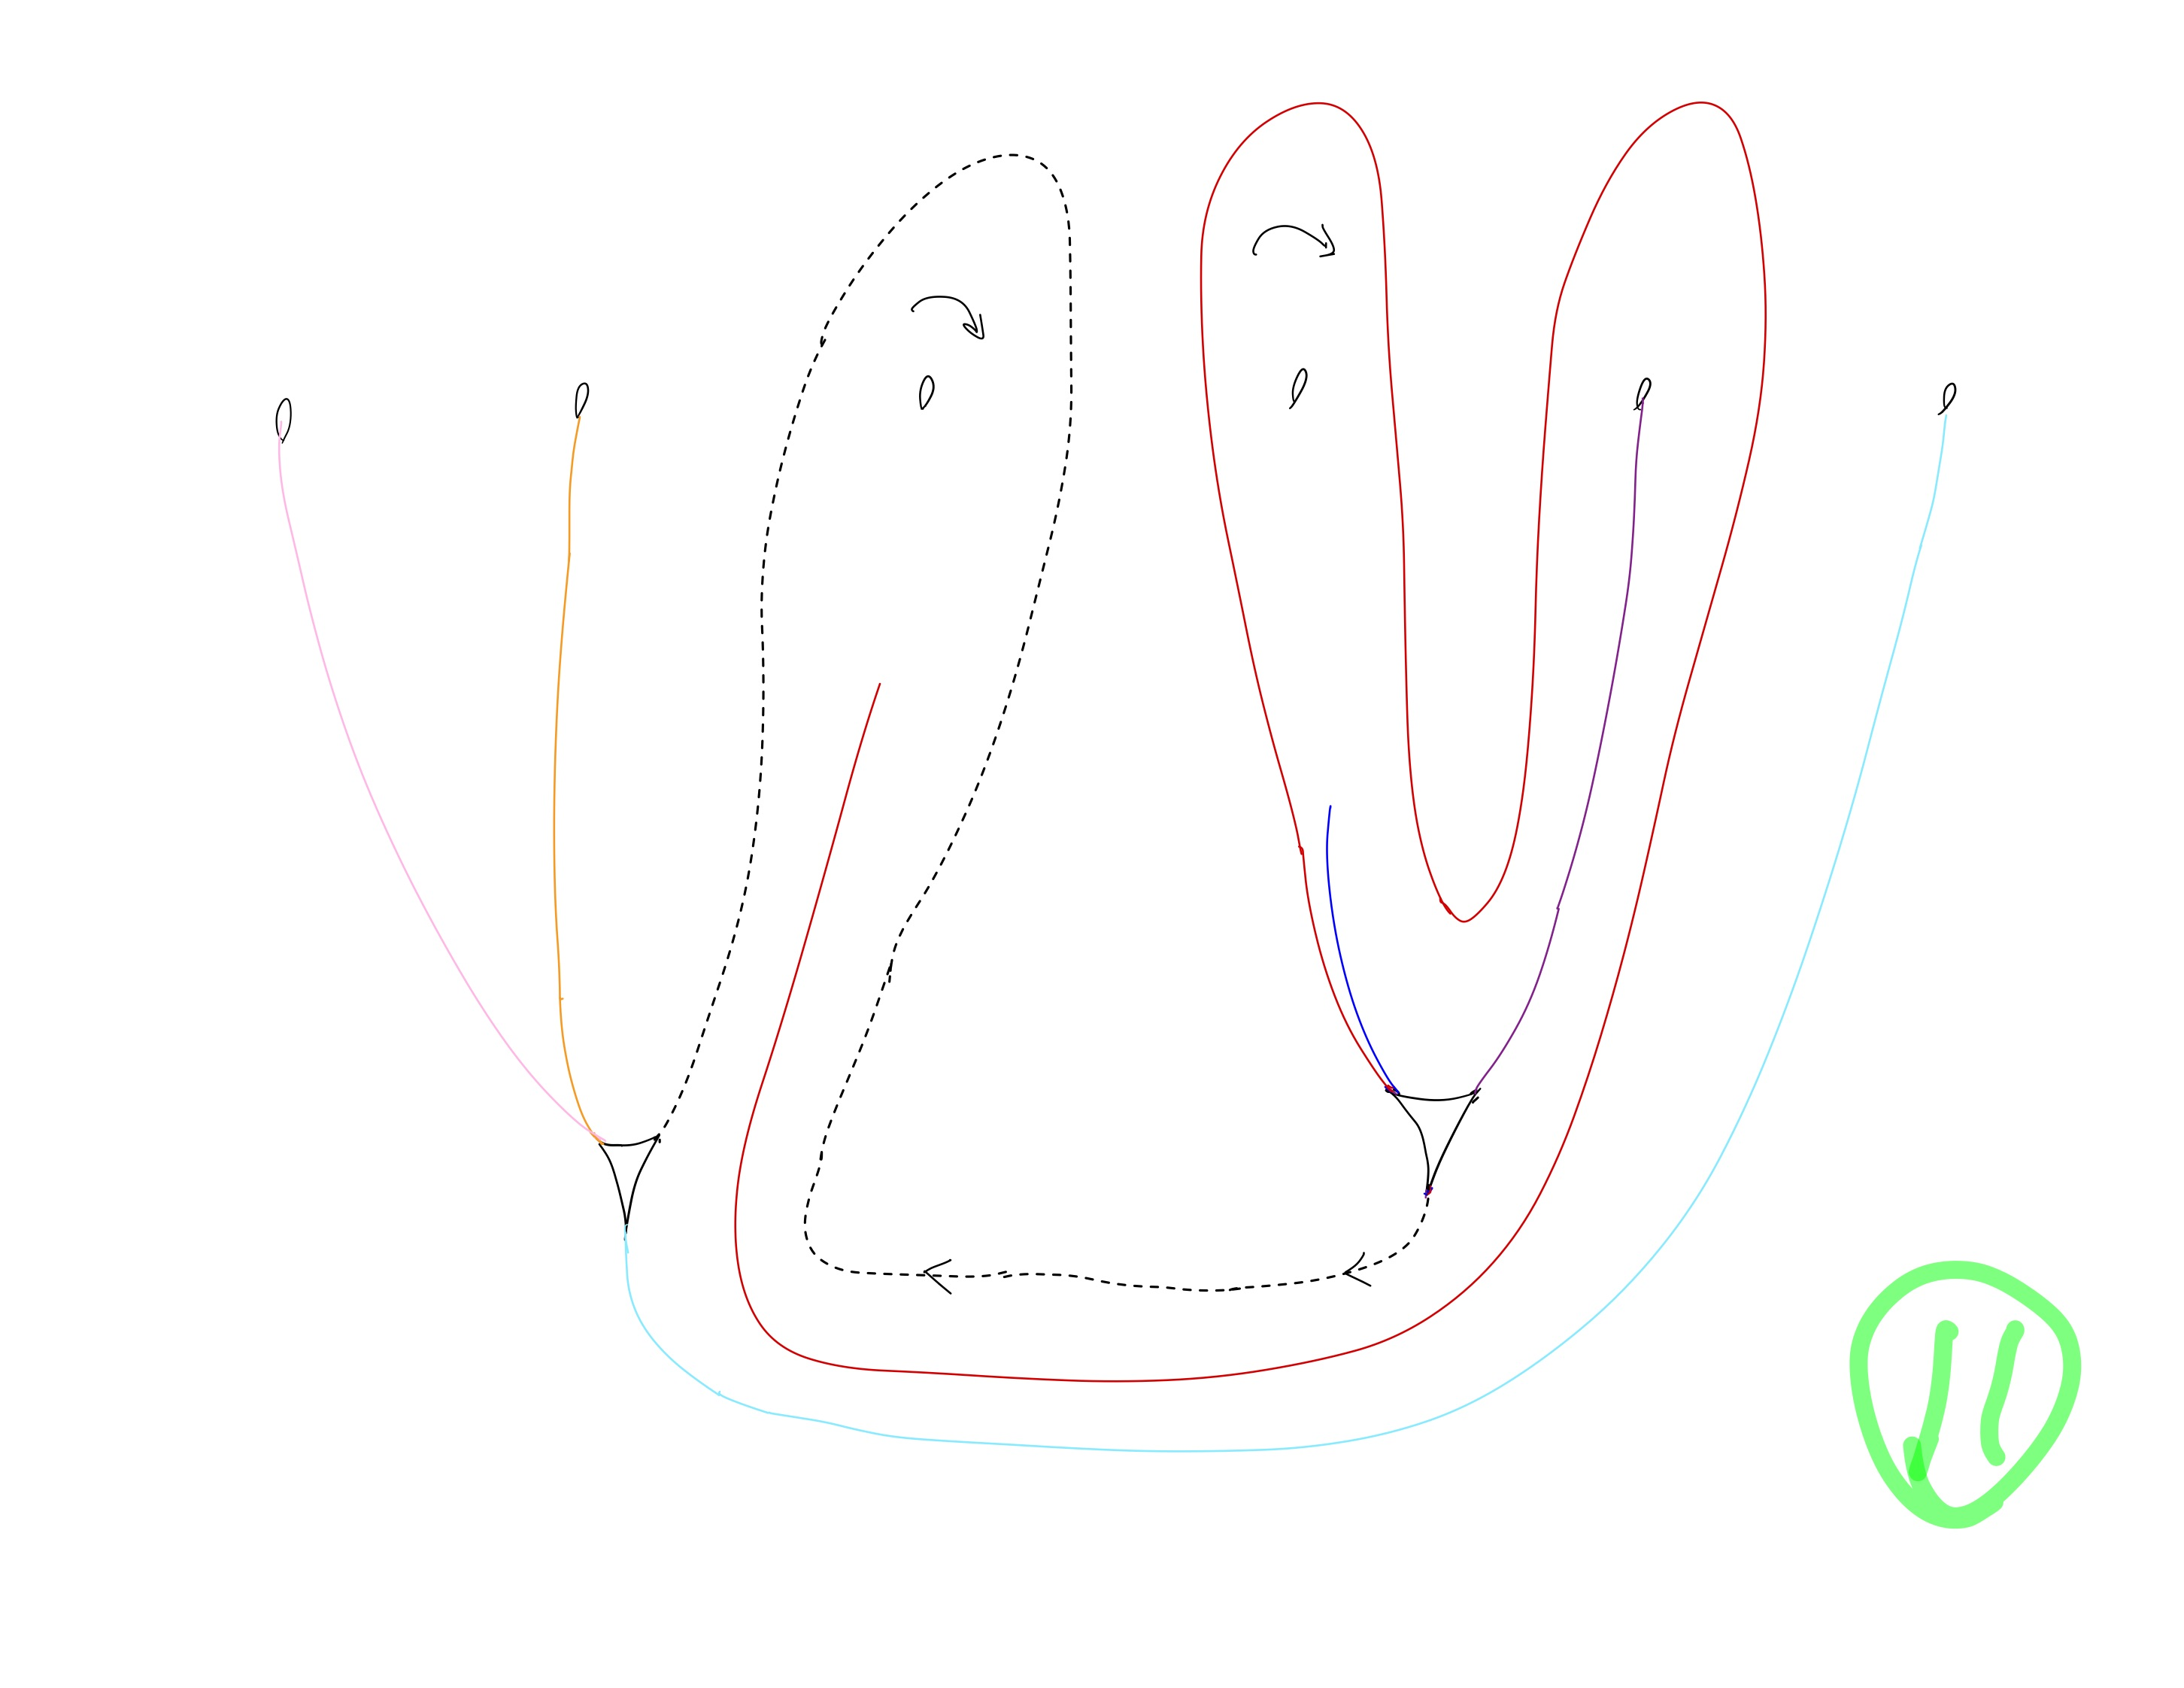
\includegraphics[width=\linewidth, height=0.45\textheight, keepaspectratio]{figures_braid/figures_track_0/Track 0 Braid 11 Jubilant-1.jpg}
    \caption{Train Track Map Candidate Family 11 of Track 0.}
    \label{fig:track0_braid_b0_11_map}
\end{figure*}

The inverse of the following braid carries this family of train track maps:
\[
b_{11}^0 = \sigma_{4} \sigma_{3} \sigma_{4}^k \sigma_{4} \sigma_{3} \sigma_{4} \sigma_{2} \sigma_{1} \sigma_{3} \sigma_{2} \sigma_{4} \sigma_{3} \sigma_{5} \sigma_{4} \sigma_{5} \sigma_{5}
\]
where $k \geq 1$ ($k \in \mathbb{Z}$) is the twisting parameter. This is shown in Figure \ref{fig:track0_braid_b0_11}.

\begin{figure*}[p]
    \centering
    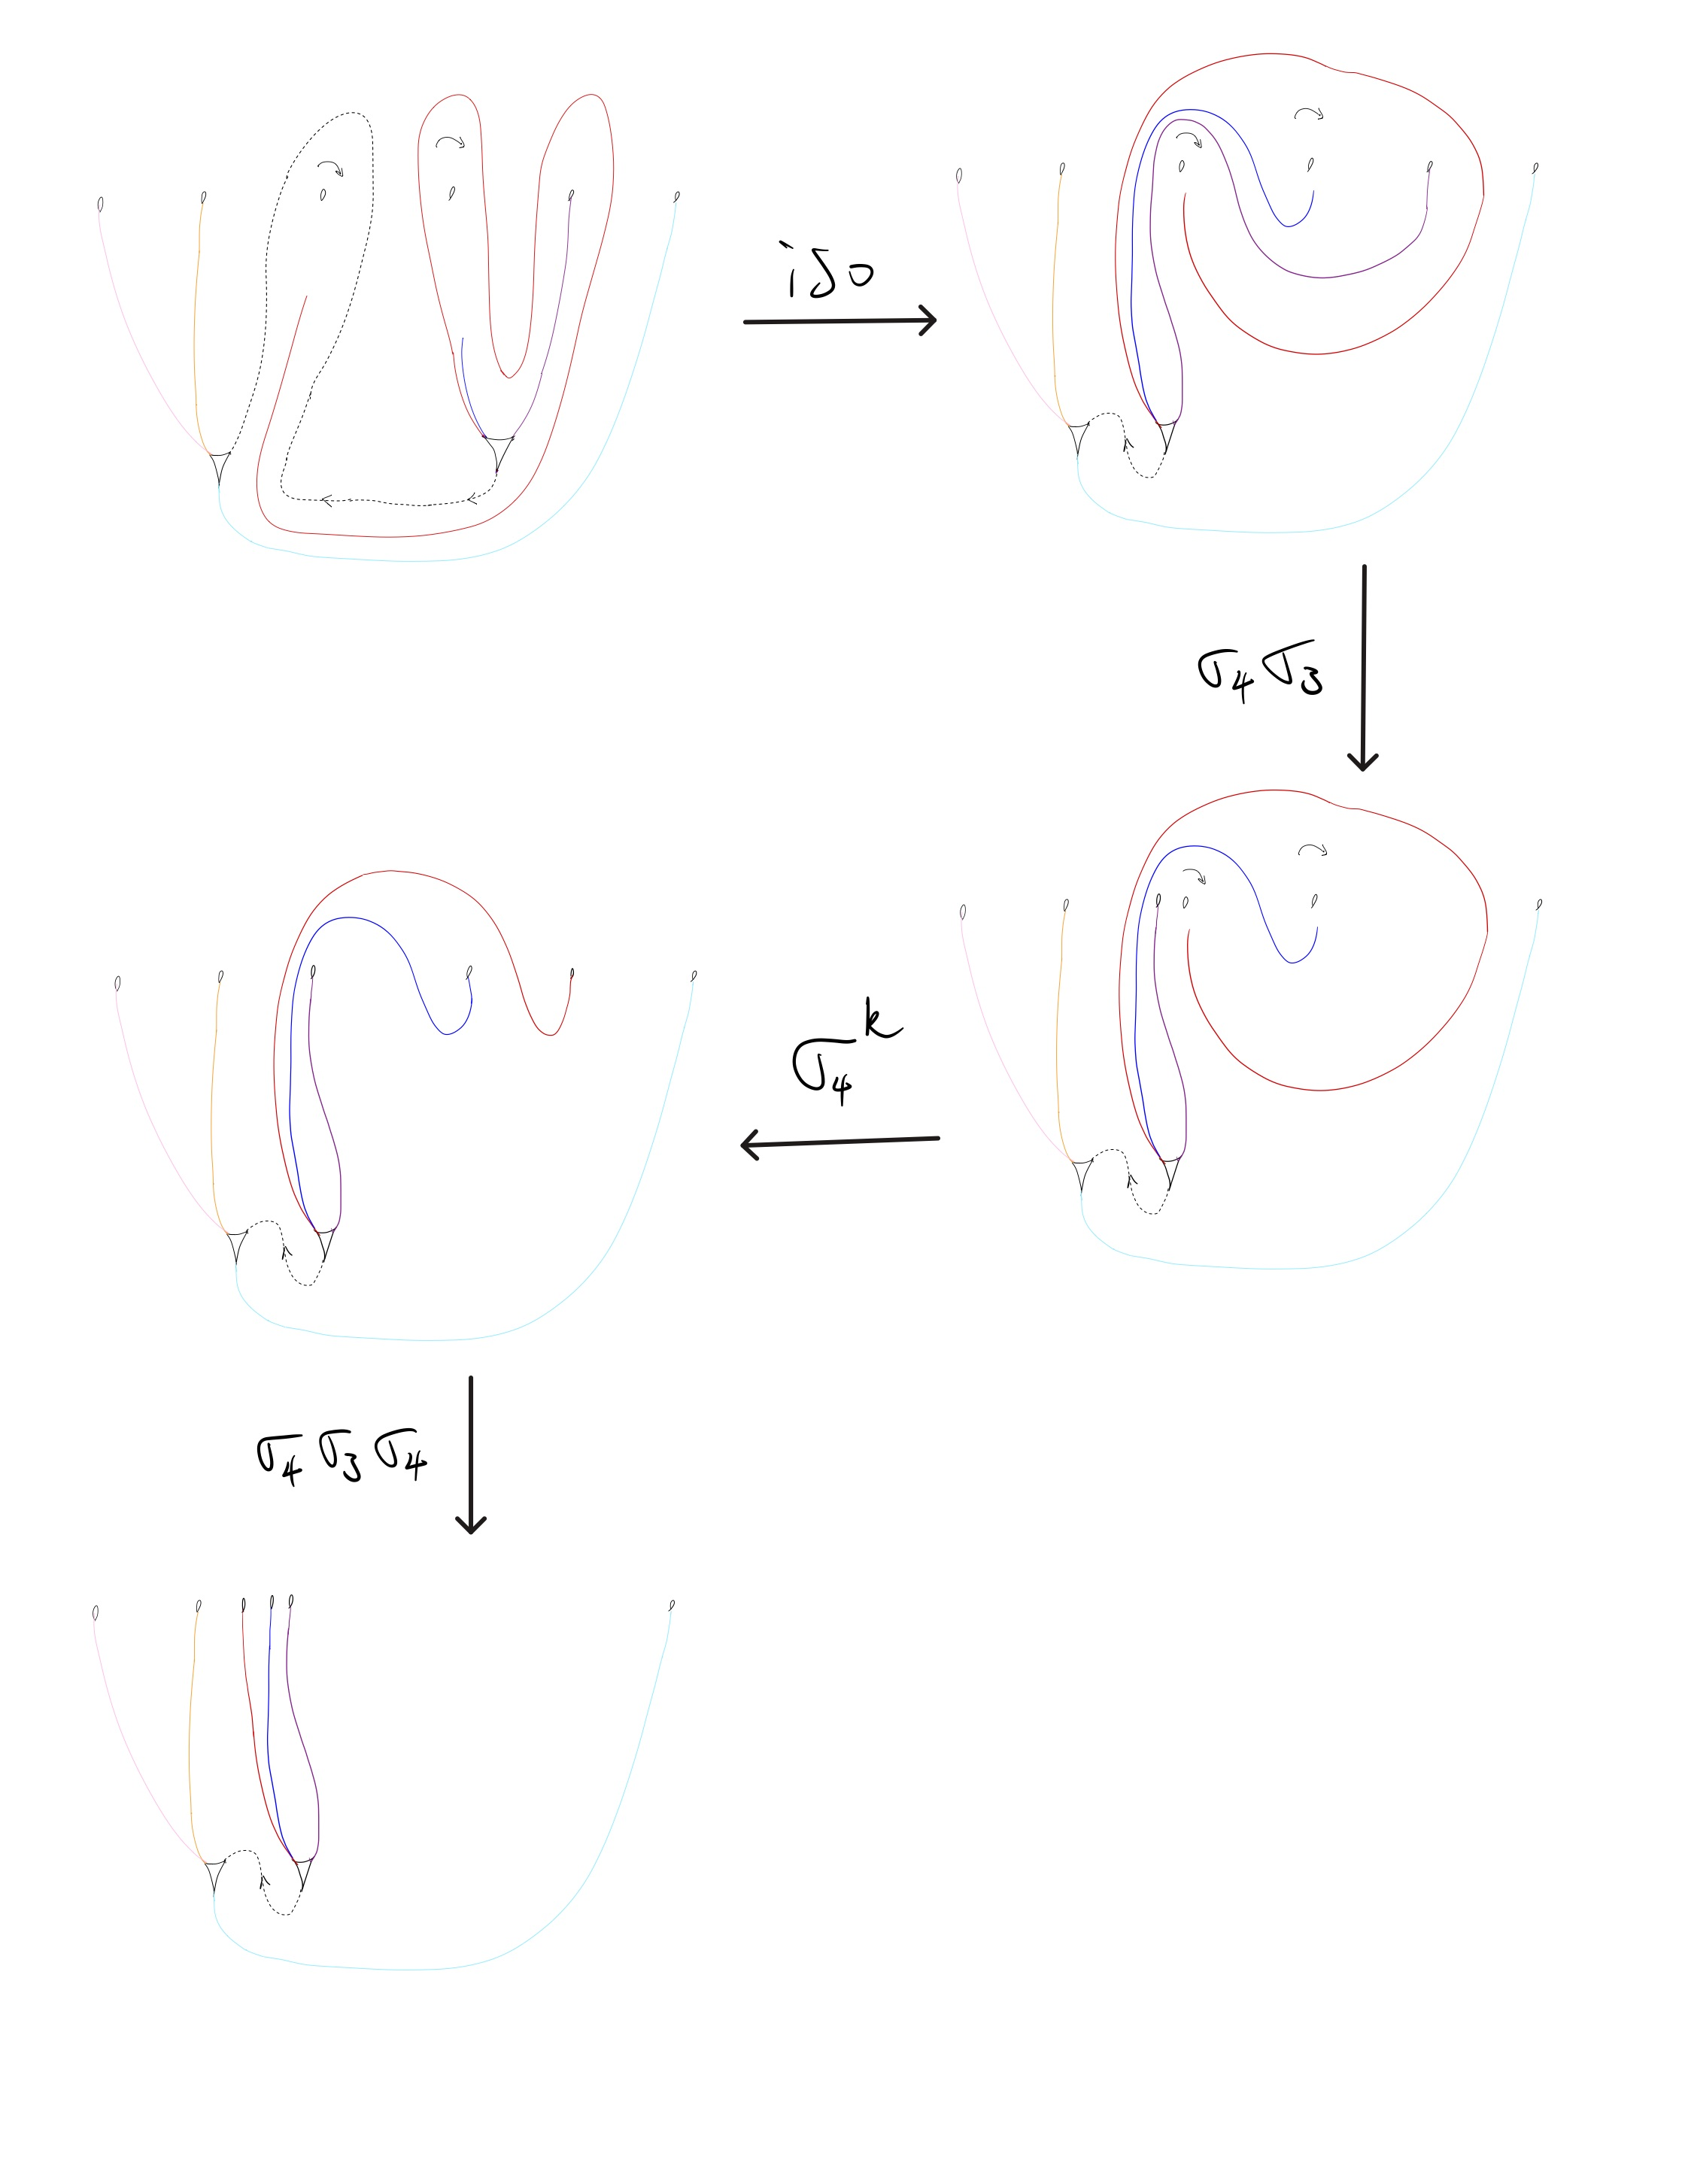
\includegraphics[width=\linewidth, height=0.45\textheight, keepaspectratio]{figures_braid/figures_track_0/Track 0 Braid 11 Jubilant-2.jpg}\\
    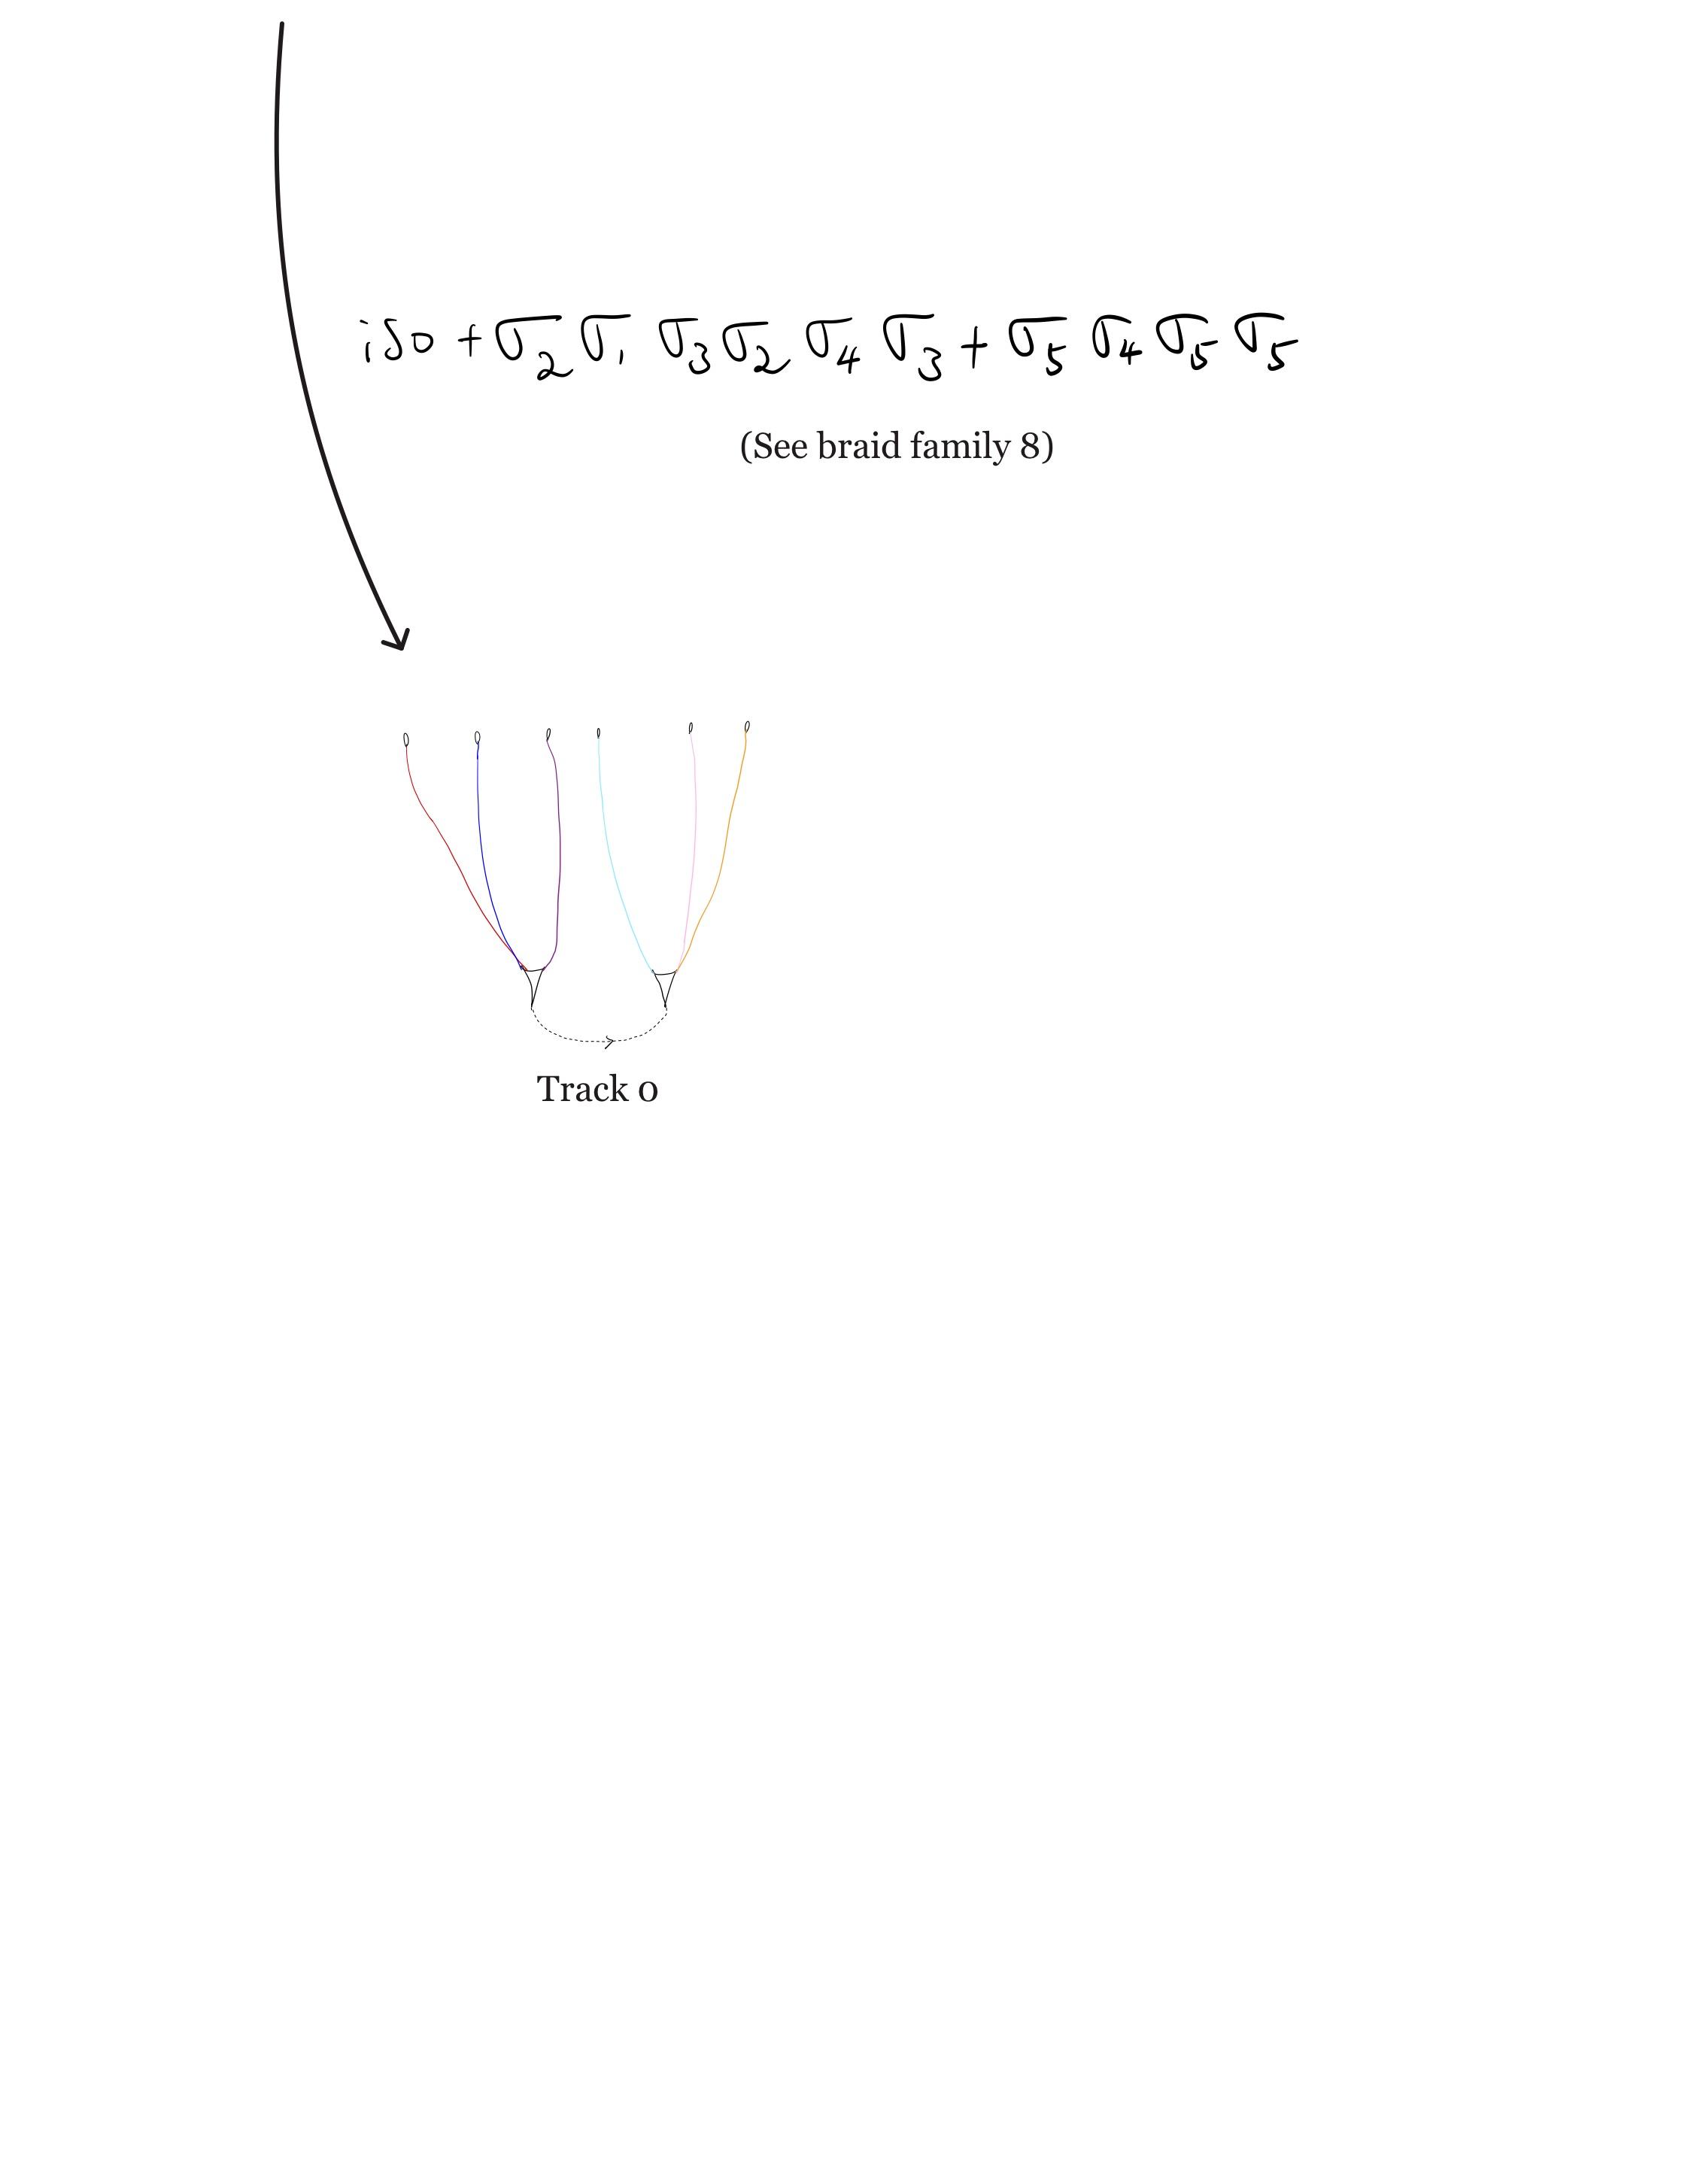
\includegraphics[width=\linewidth, height=0.45\textheight, keepaspectratio]{figures_braid/figures_track_0/Track 0 Braid 11 Jubilant-3.jpg}
    \caption{This sequence shows the inverse of the braid $b_{11}^0$ carries Train Track Candidate Family 11.}
    \label{fig:track0_braid_b0_11}
\end{figure*}

\clearpage

\section{Candidate Family 12 (Jubilant)}\label{sec:track0_jubilant_2}
Train Track Map Candidate Family 12 of Track 0 is shown in Figure \ref{fig:track0_braid_b0_12_map}. See \ref{Jubilant} for details.

\begin{figure*}[ht]
    \centering
    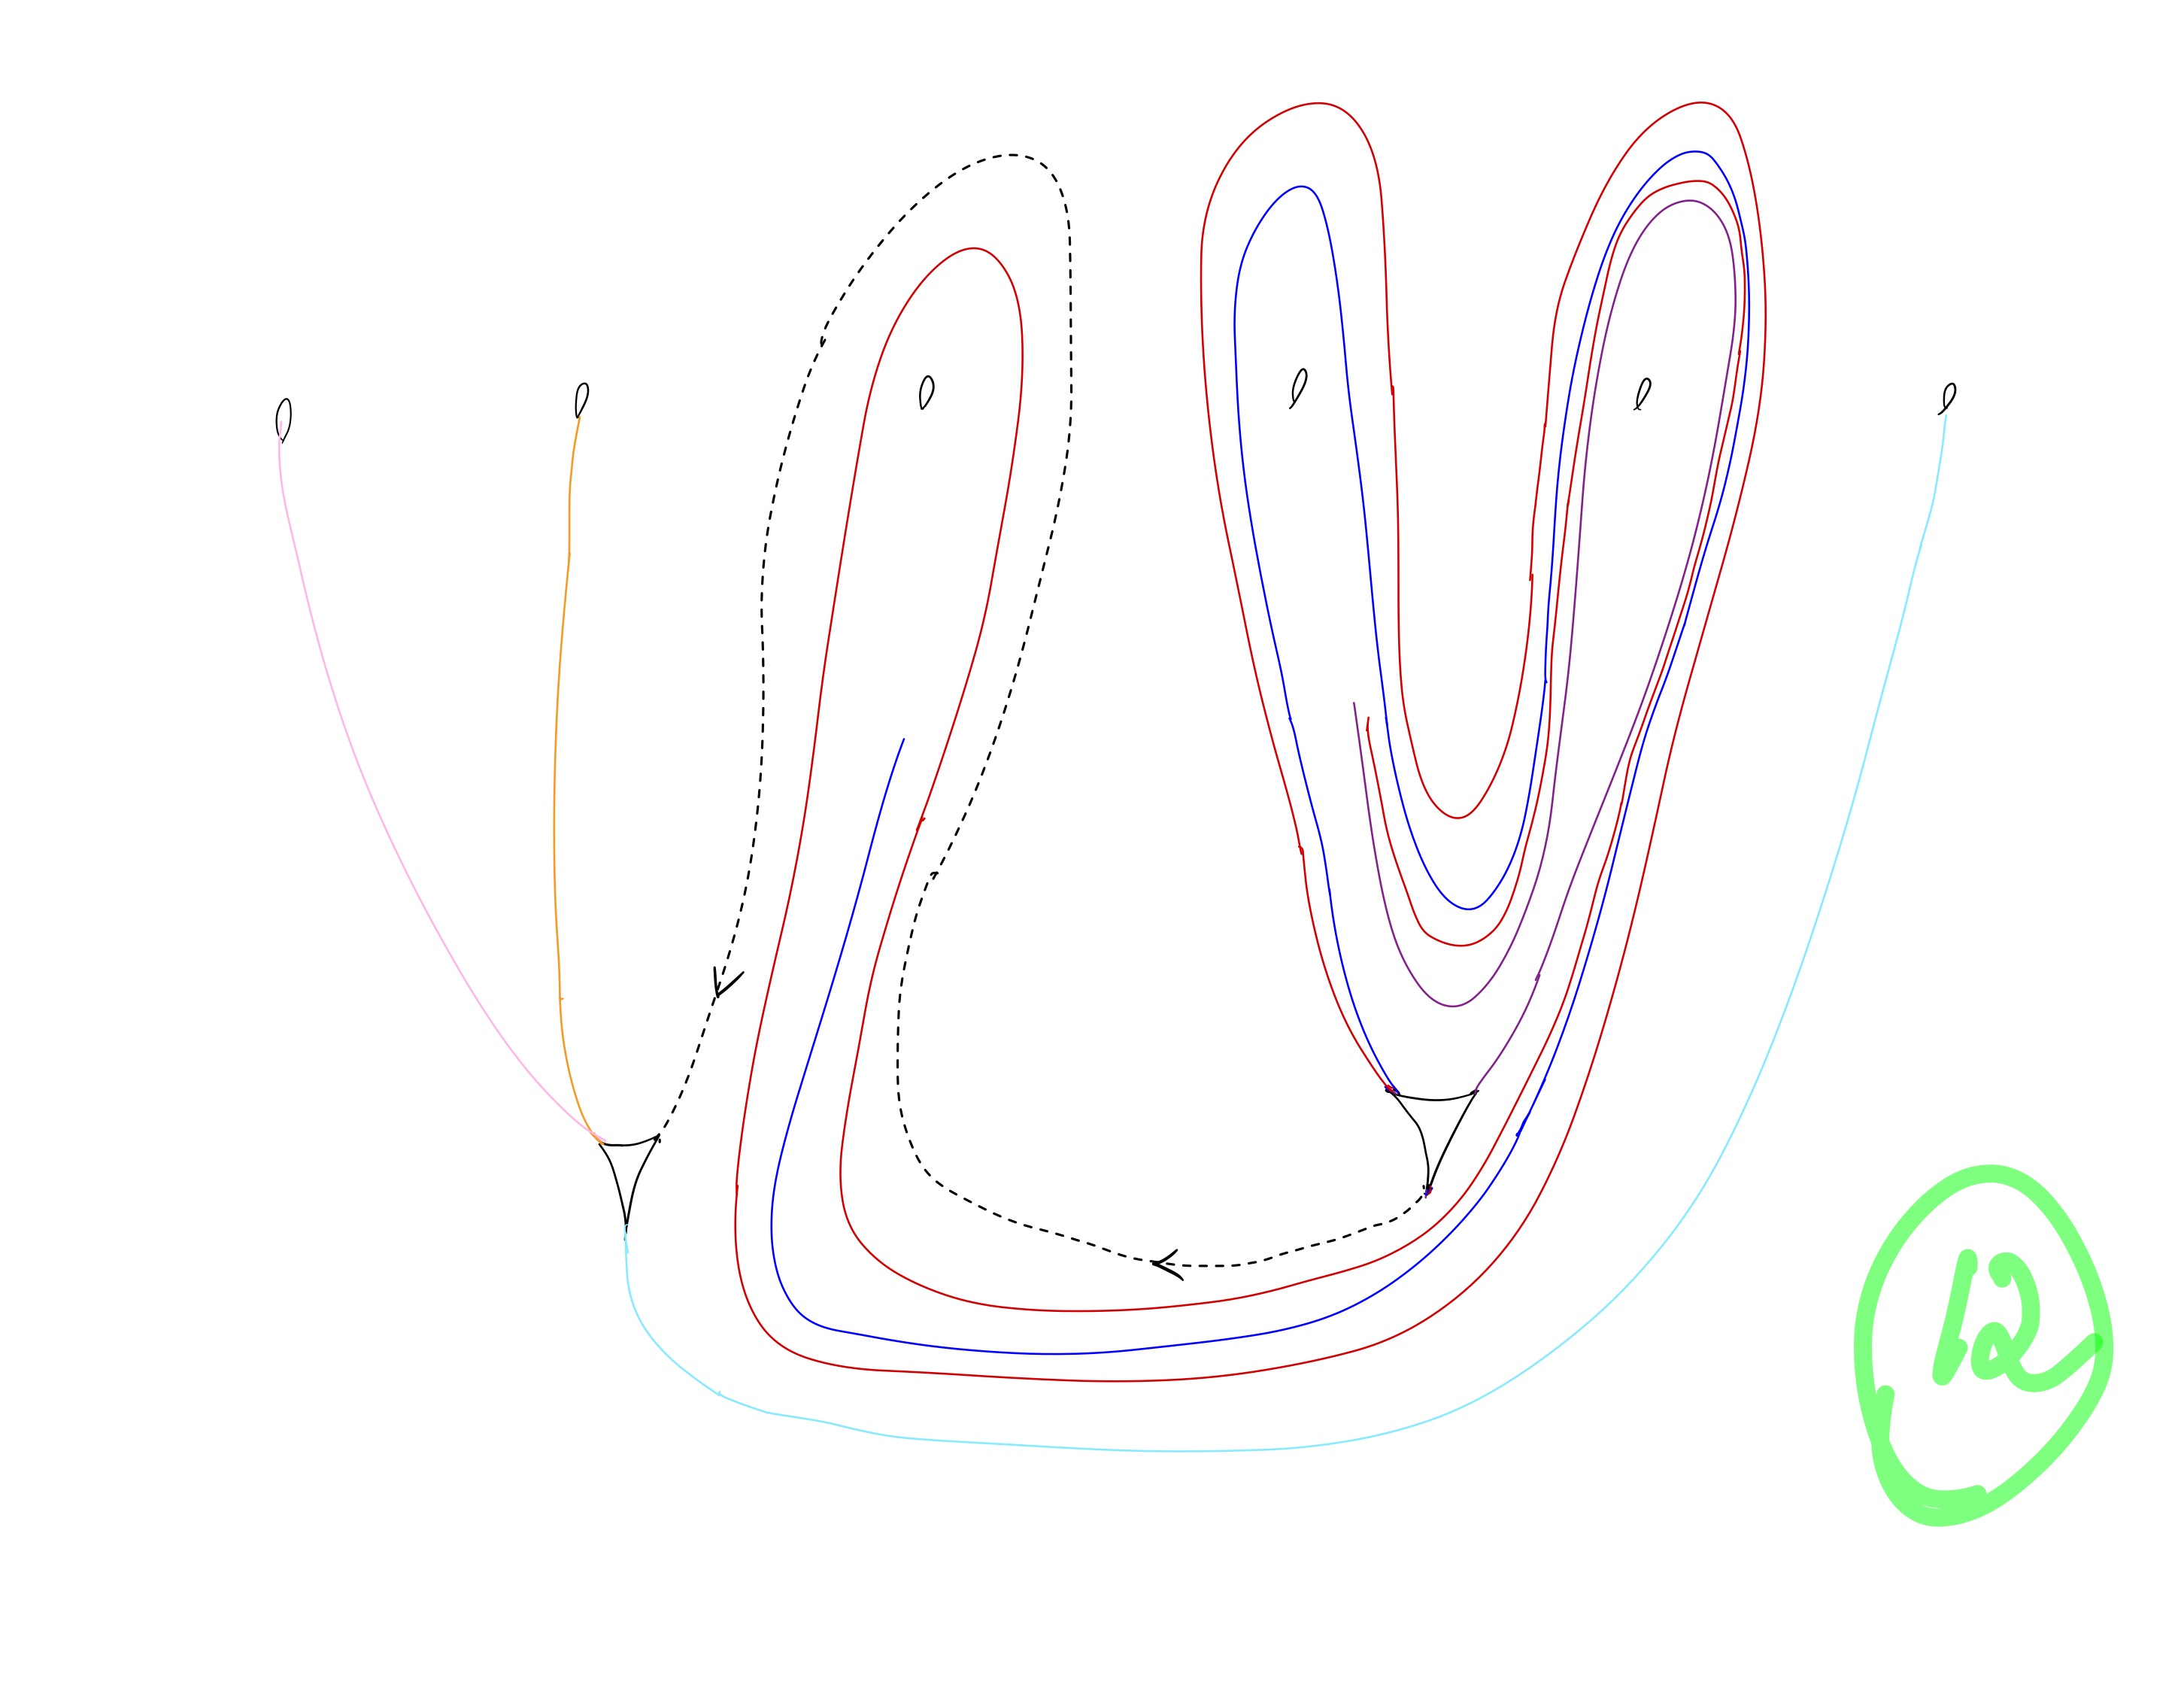
\includegraphics[width=\linewidth, height=0.45\textheight, keepaspectratio]{figures_braid/figures_track_0/Track 0 Braid 12 Jubilant-1.jpg}
    \caption{Train Track Map Candidate Family 12 of Track 0.}
    \label{fig:track0_braid_b0_12_map}
\end{figure*}

The inverse of the following braid carries this family of train track maps:
\[
b_{12}^0 = \sigma_{4}^{-k} \sigma_{4}^{-1} \sigma_{3} \sigma_{4}^m \sigma_{4} \sigma_{3} \sigma_{4} \sigma_{1} \sigma_{3} \sigma_{2} \sigma_{4} \sigma_{3} \sigma_{5} \sigma_{4} \sigma_{5} \sigma_{5}
\]
where $k, m \geq 1$ ($k, m \in \mathbb{Z}$) are the twisting parameters. This is shown in Figure \ref{fig:track0_braid_b0_12}.

\begin{figure*}[p]
    \centering
    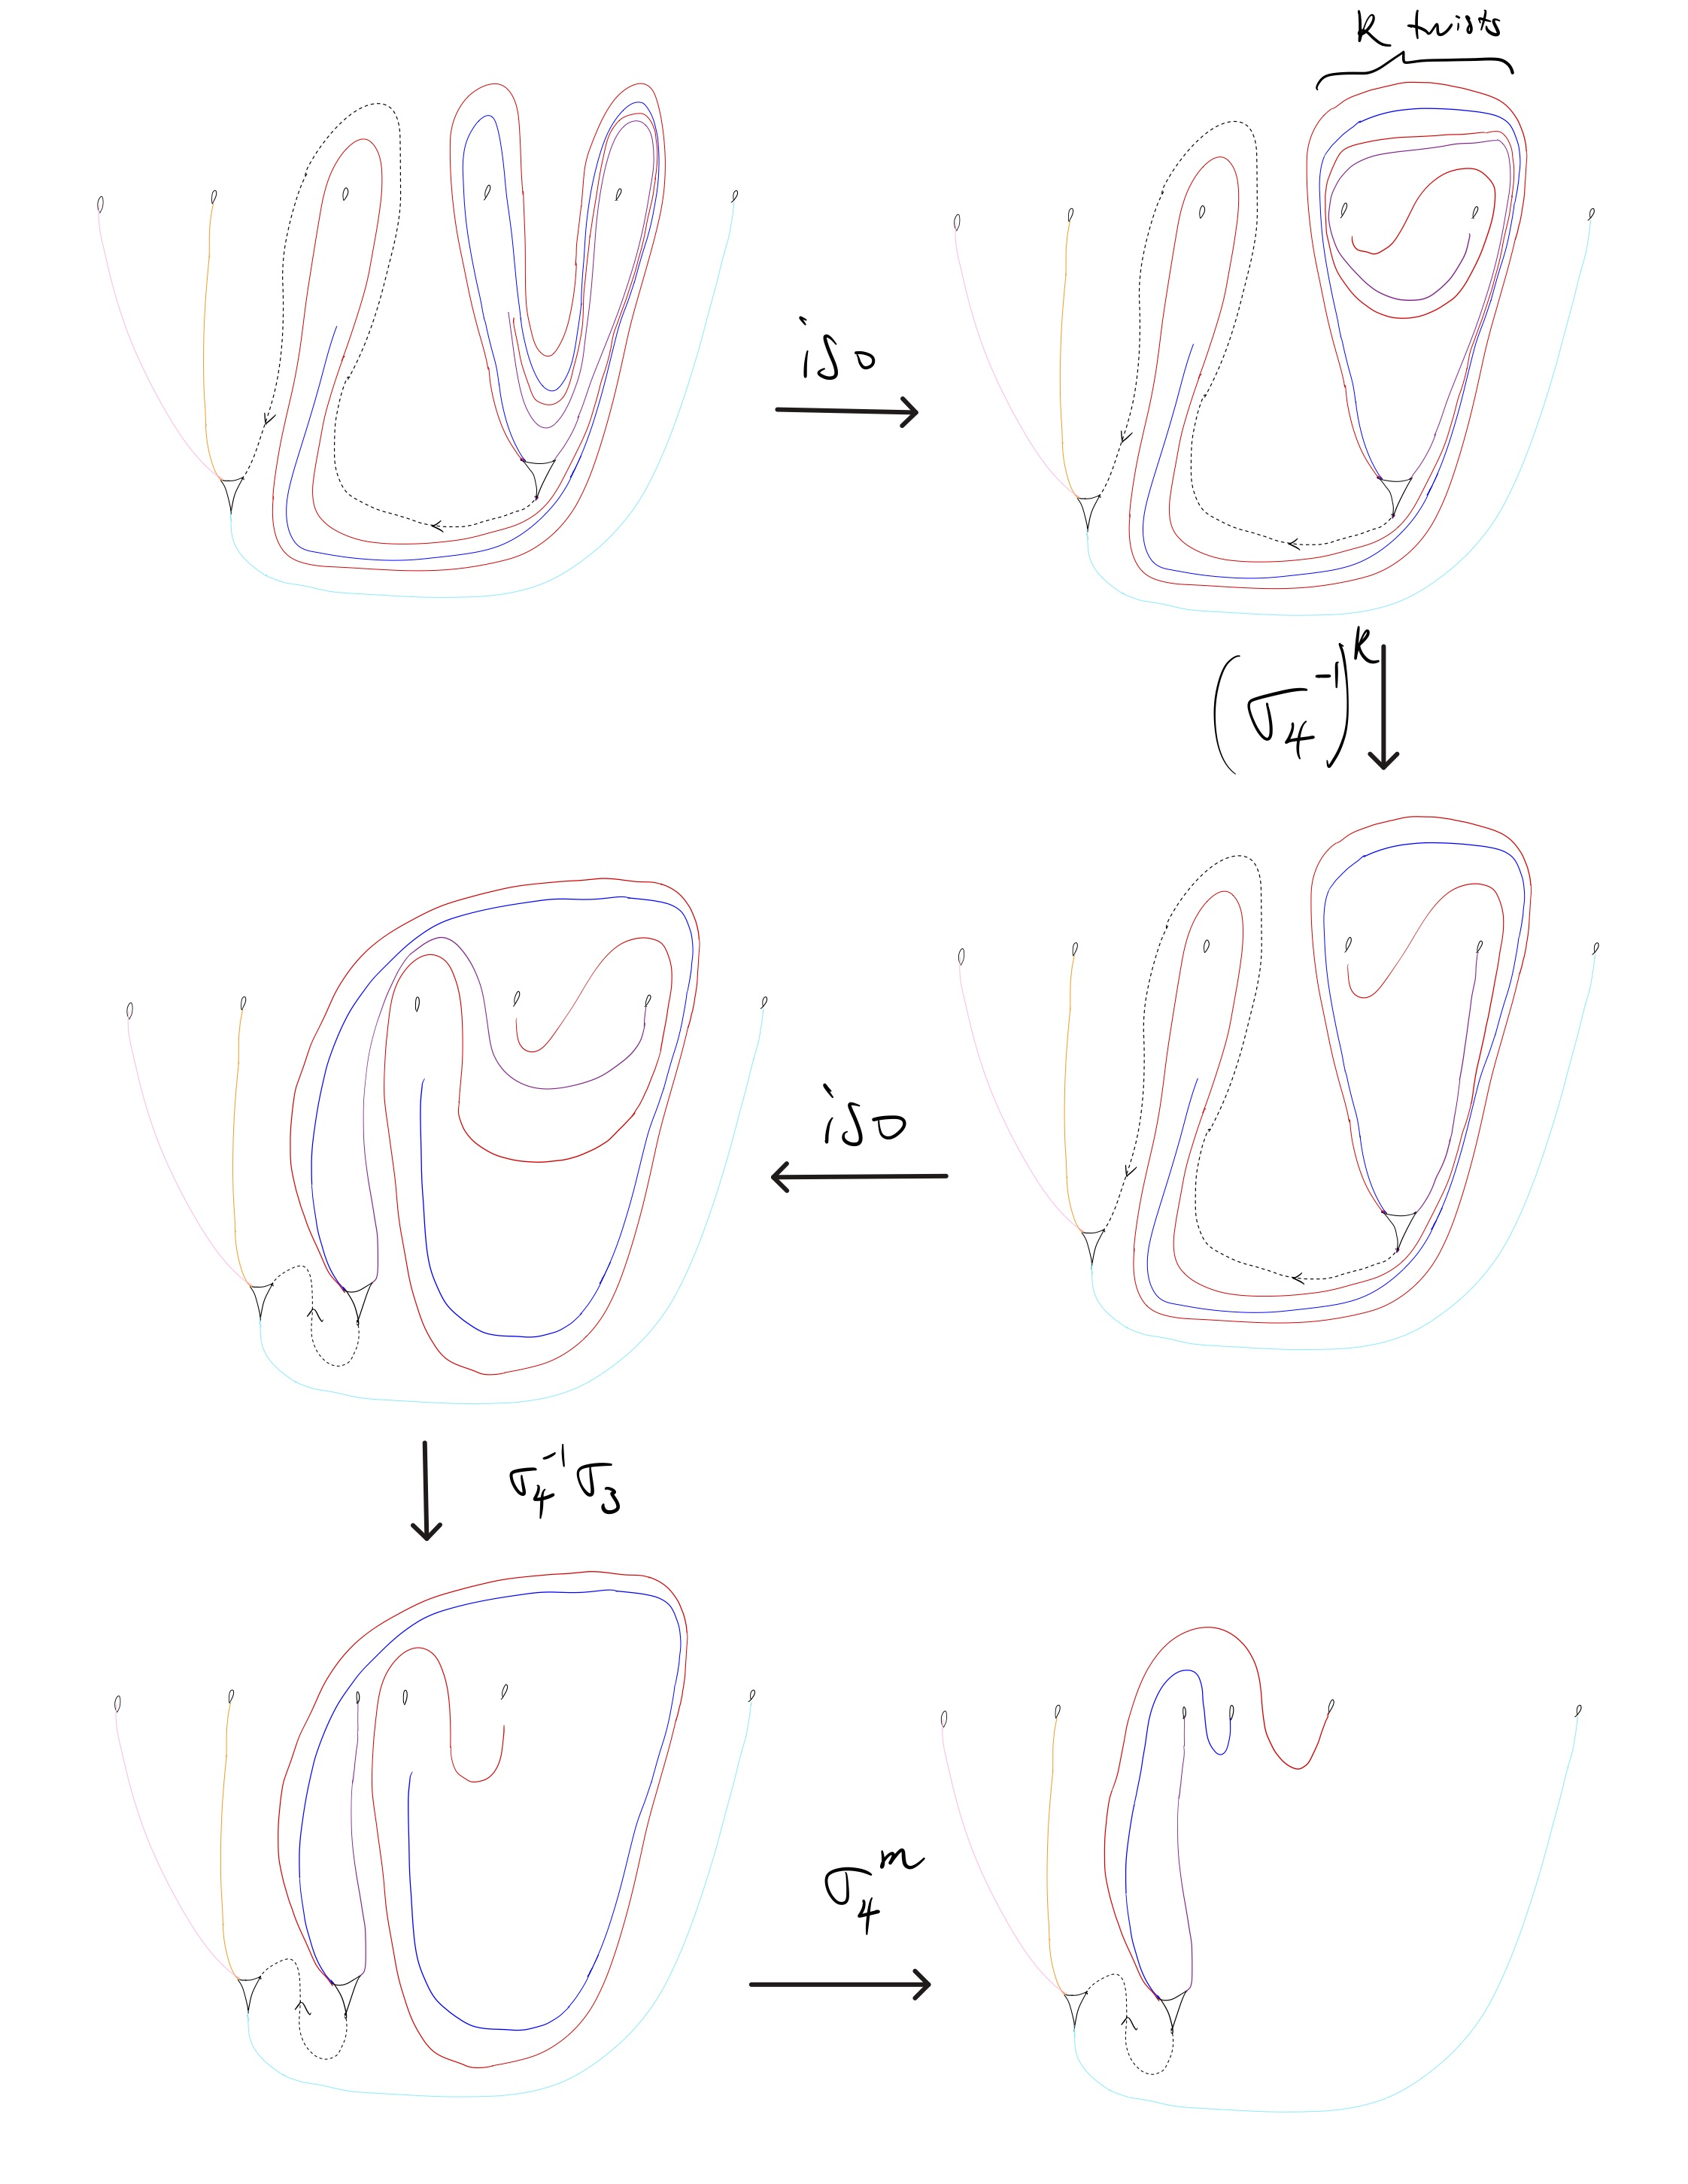
\includegraphics[width=\linewidth, height=0.45\textheight, keepaspectratio]{figures_braid/figures_track_0/Track 0 Braid 12 Jubilant-2.jpg}\\
    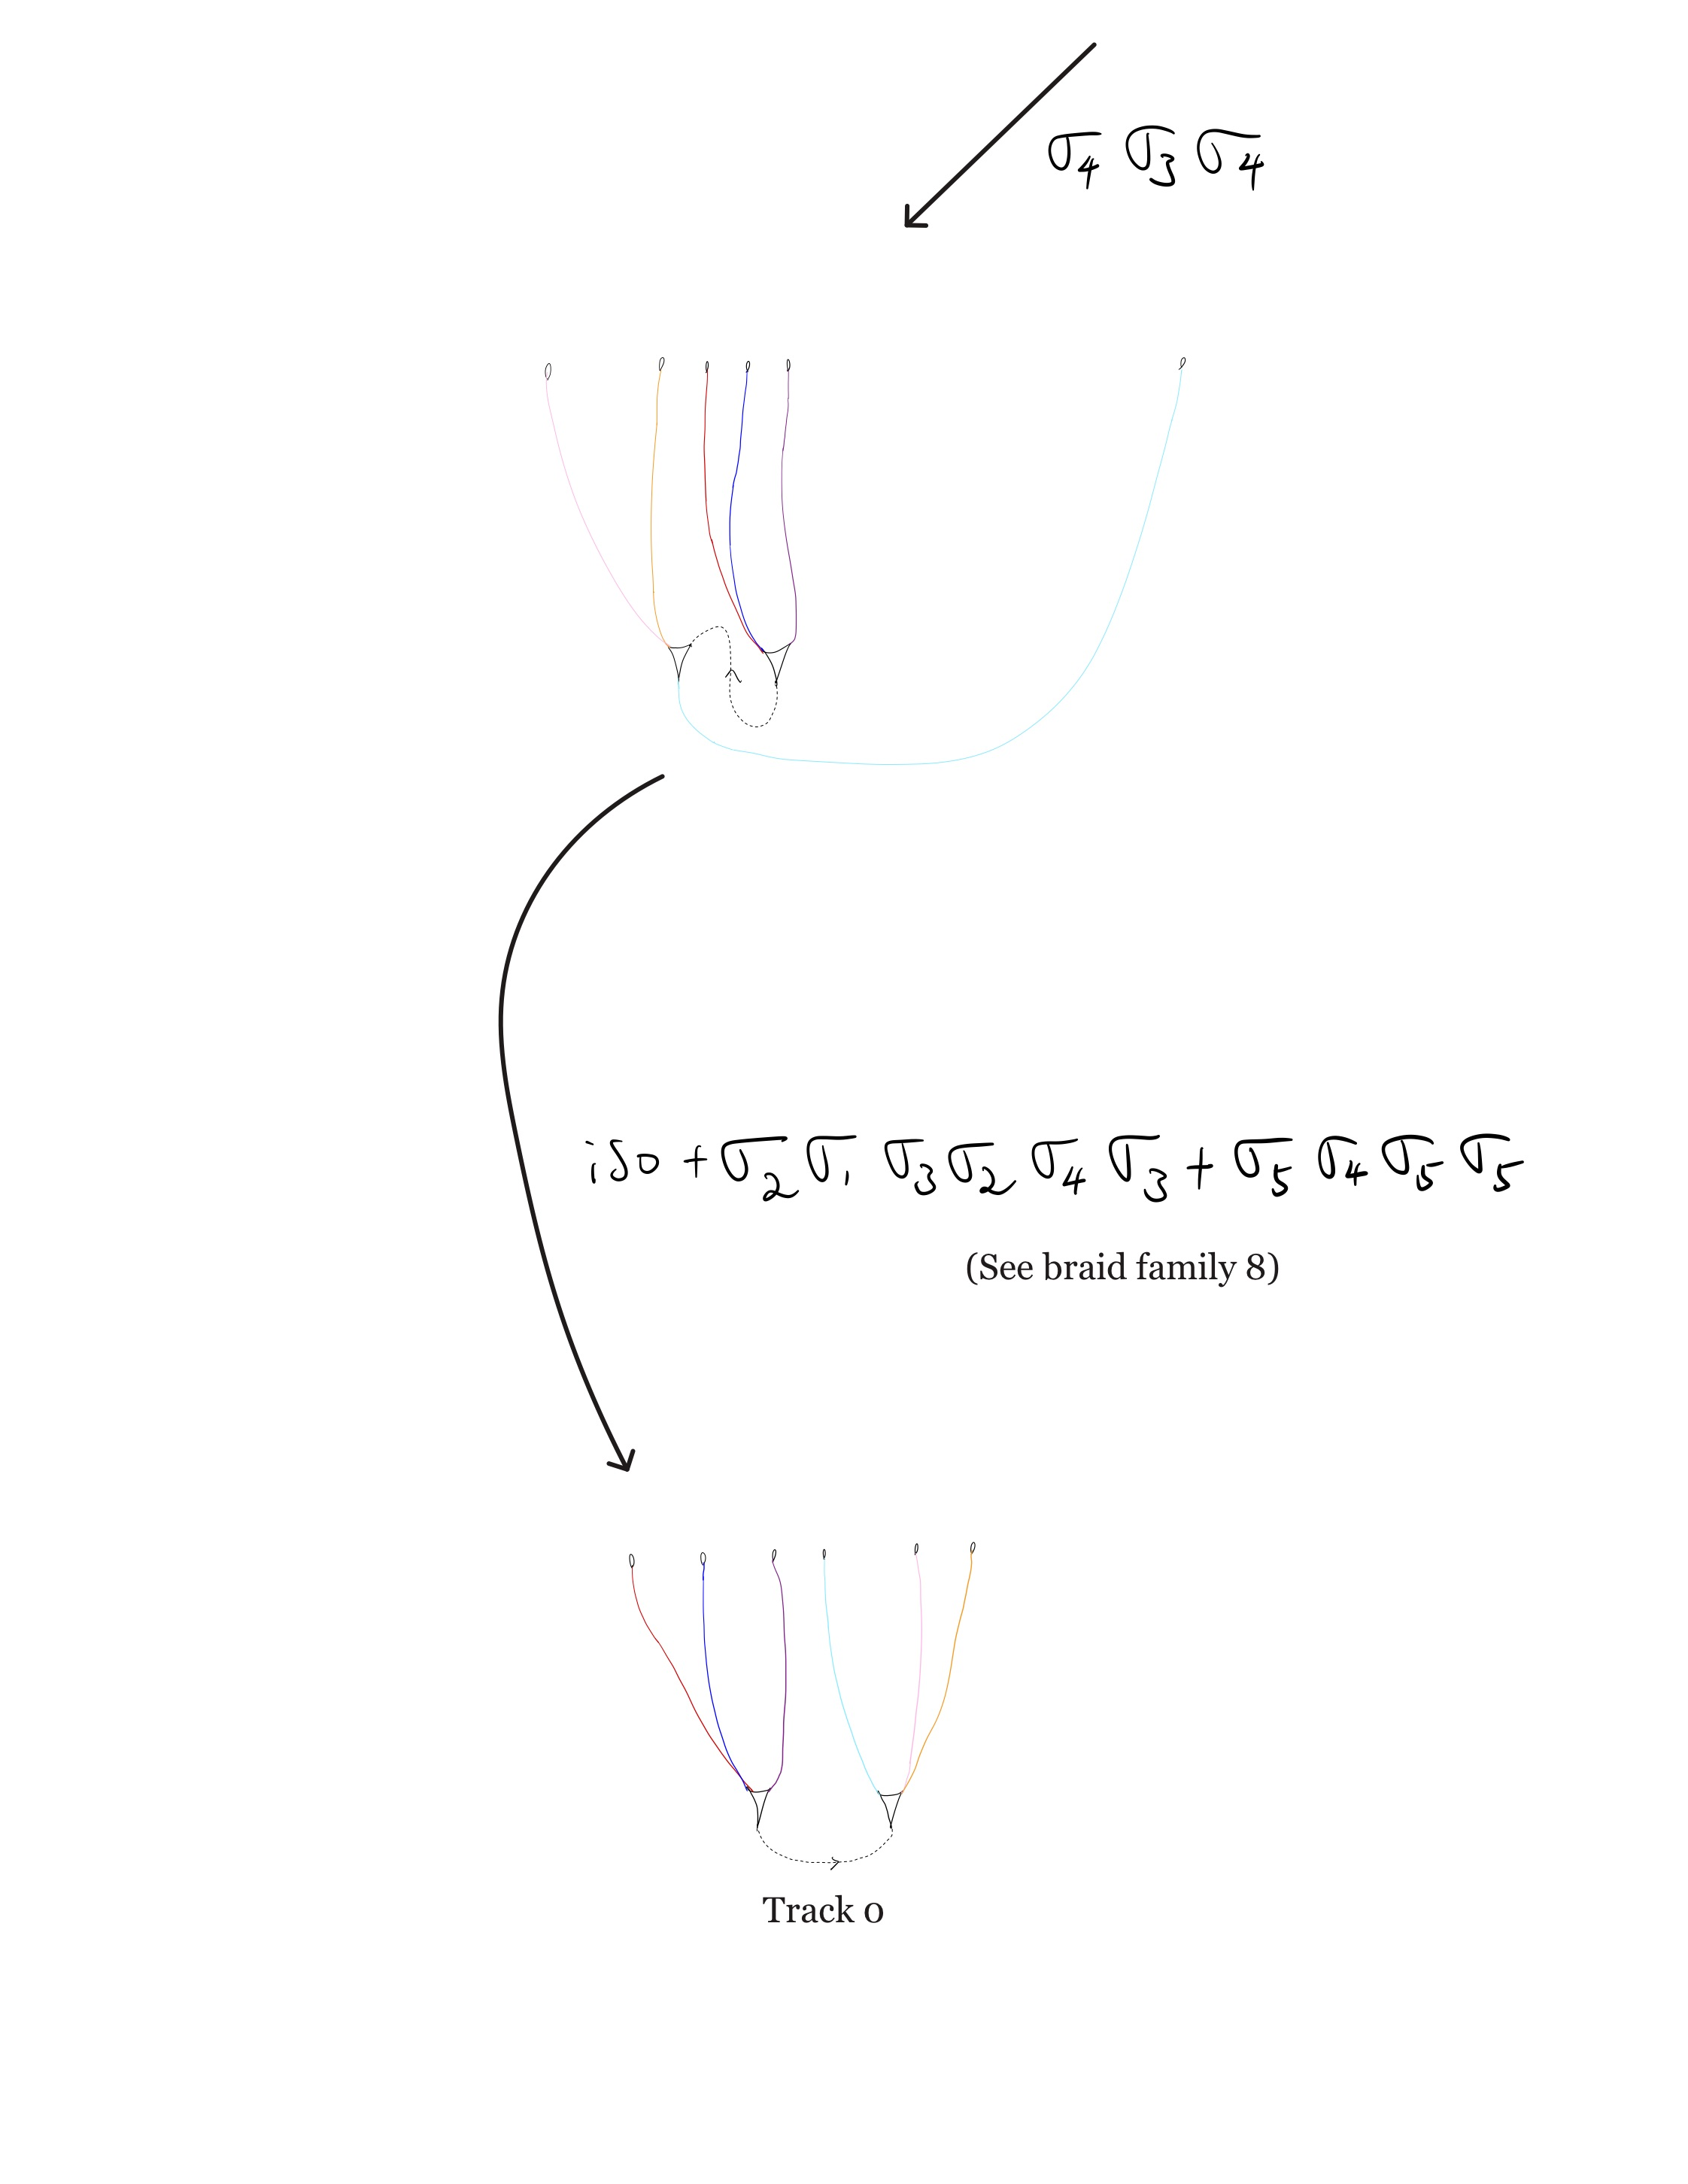
\includegraphics[width=\linewidth, height=0.45\textheight, keepaspectratio]{figures_braid/figures_track_0/Track 0 Braid 12 Jubilant-3.jpg}
    \caption{This sequence shows the inverse of the braid $b_{12}^0$ carries Train Track Candidate Family 12.}
    \label{fig:track0_braid_b0_12}
\end{figure*}

\clearpage

\section{Candidate Family 13 (Treasure)}\label{sec:track0_treasure}
Train Track Map Candidate Family 13 of Track 0 is shown in Figure \ref{fig:track0_braid_b0_13_map}. See \ref{Treasure} for details.

\begin{figure*}[ht]
    \centering
    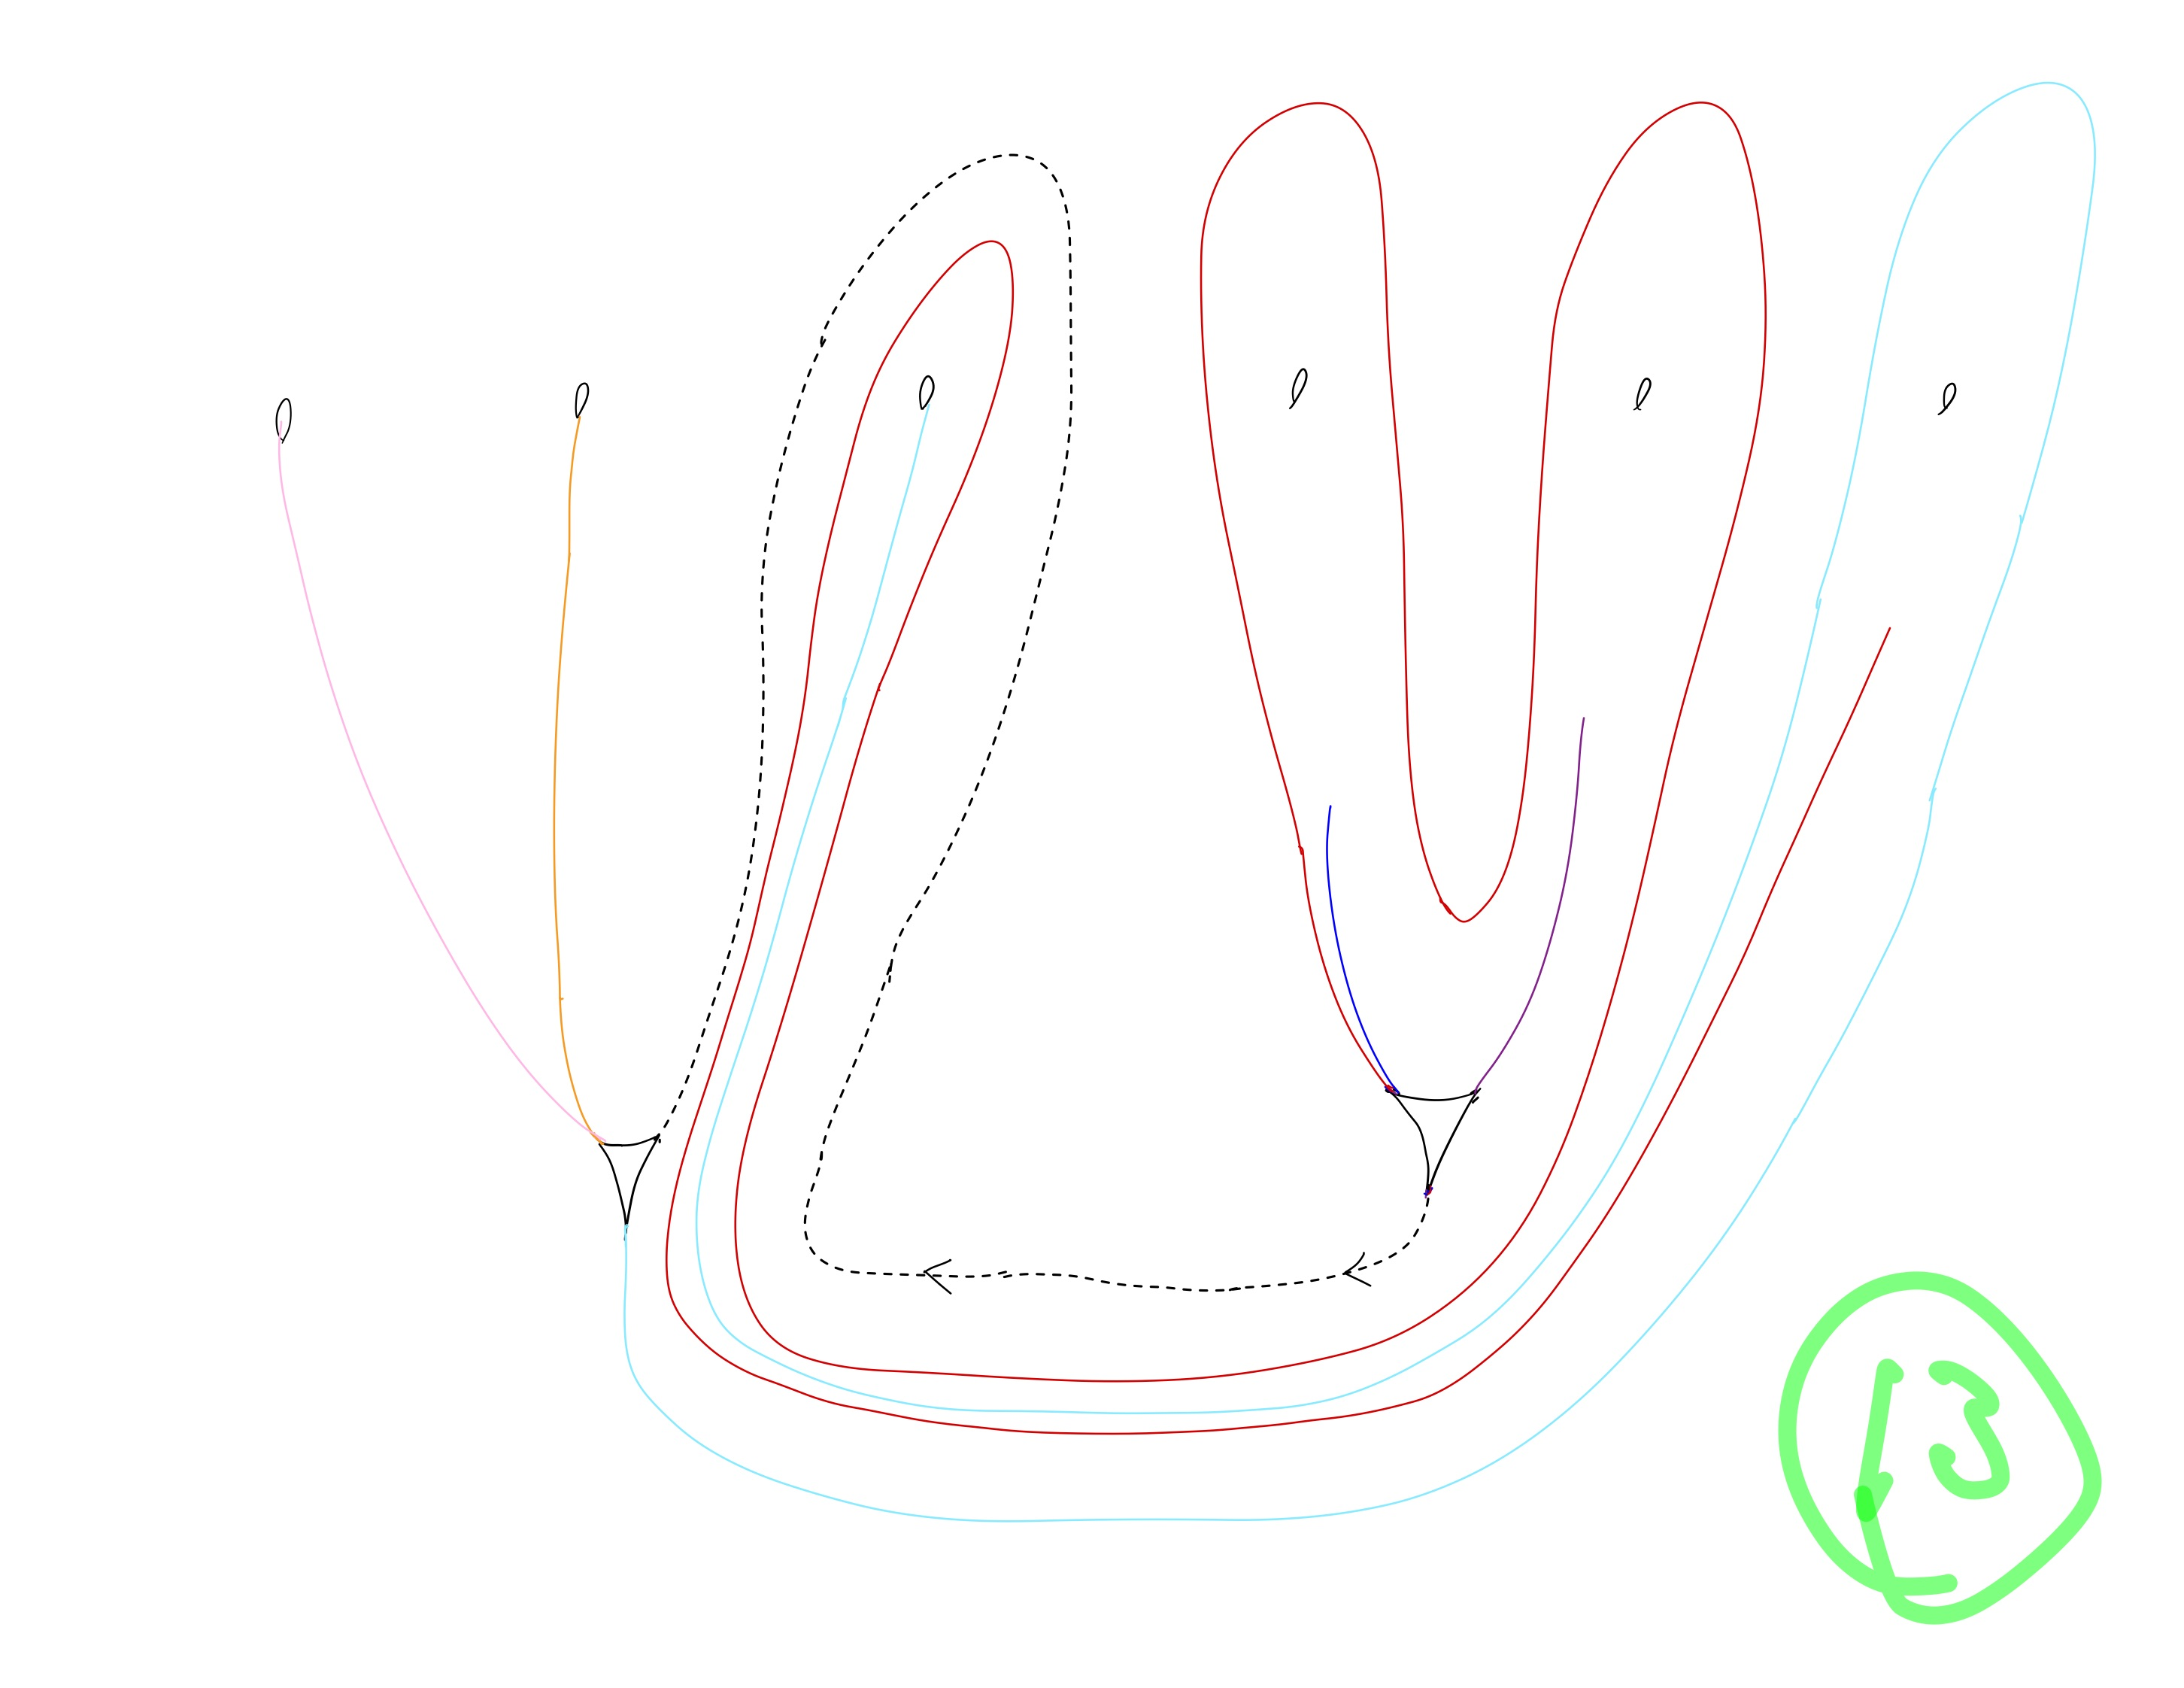
\includegraphics[width=\linewidth, height=0.45\textheight, keepaspectratio]{figures_braid/figures_track_0/Track 0 Braid 13 Treasure-1.jpg}
    \caption{Train Track Map Candidate Family 13 of Track 0.}
    \label{fig:track0_braid_b0_13_map}
\end{figure*}

The inverse of the following braid carries this family of train track maps:
\[
b_{13}^0 = \sigma_{4}^{-k} \sigma_{4}^{-1} \sigma_{3} \sigma_{4} \sigma_{5}^{-1} \sigma_{4}^m \sigma_{3} \sigma_{4} \sigma_{2} \sigma_{1} \sigma_{3} \sigma_{2} \sigma_{4} \sigma_{3} \sigma_{5} \sigma_{4} \sigma_{5} \sigma_{5}
\]
where $k, m \geq 1$ ($k, m \in \mathbb{Z}$) are the twisting parameters. This is shown in Figure \ref{fig:track0_braid_b0_13}.

\begin{figure*}[p]
    \centering
    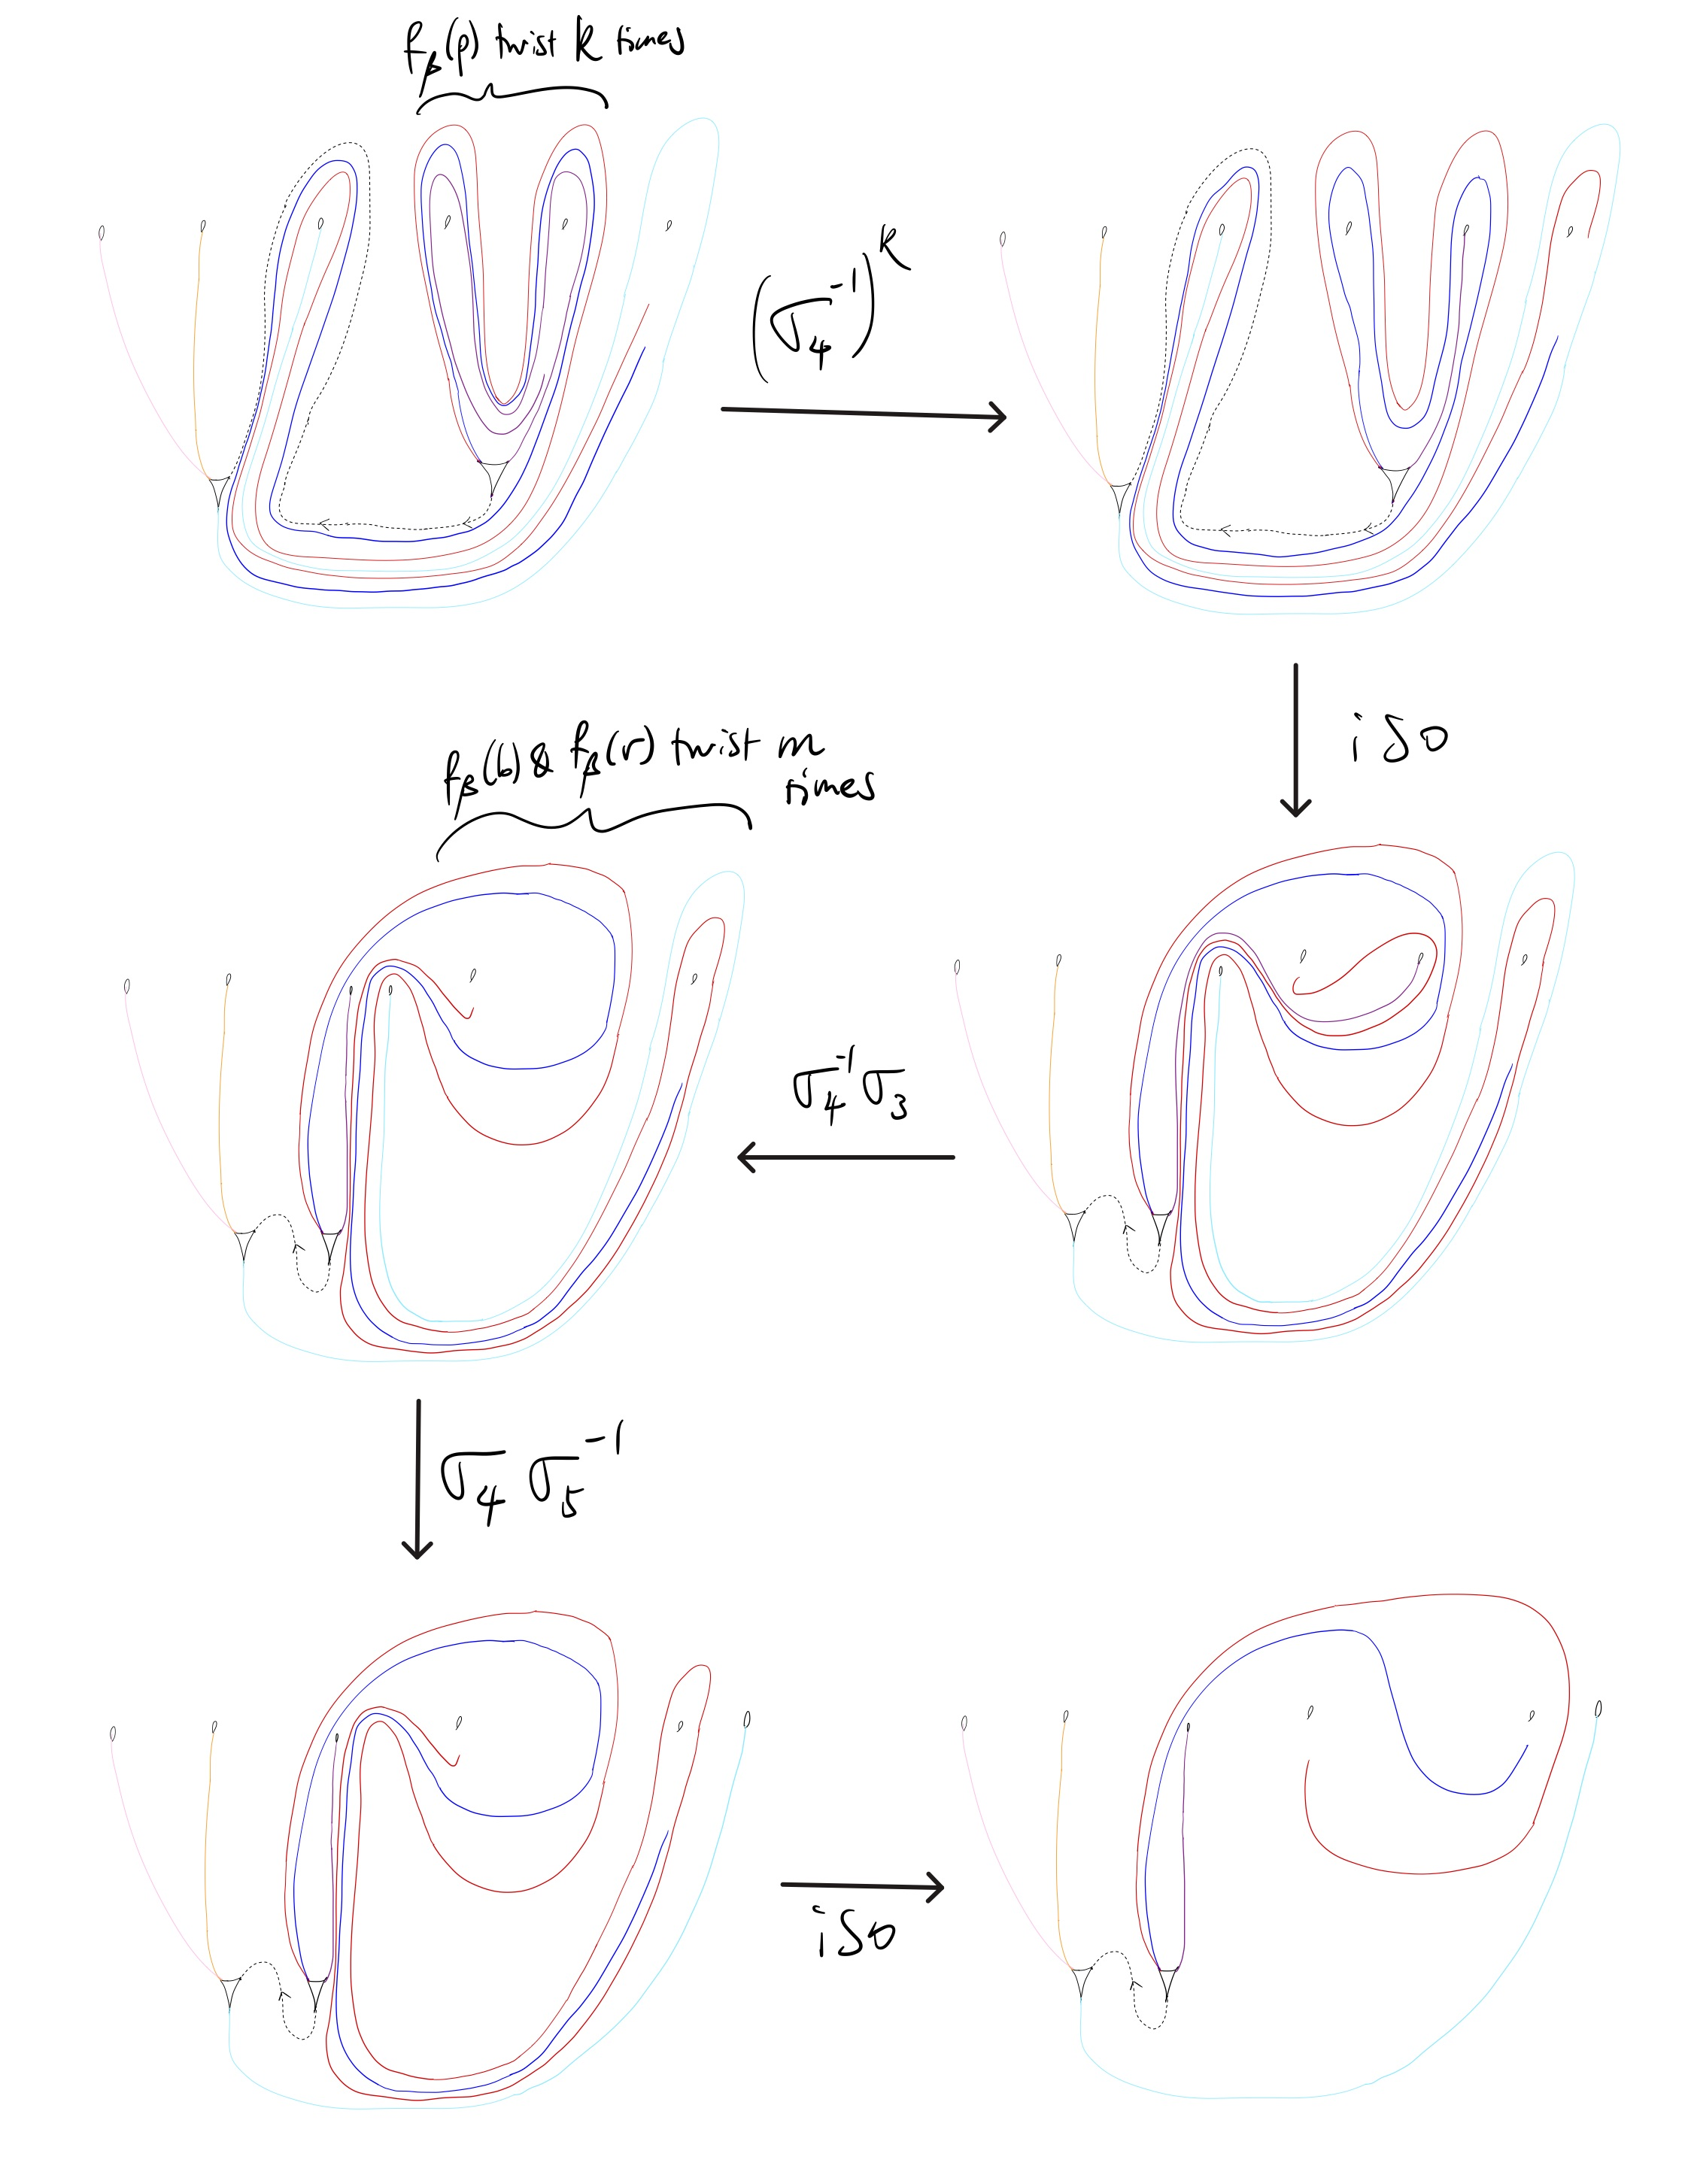
\includegraphics[width=\linewidth, height=0.45\textheight, keepaspectratio]{figures_braid/figures_track_0/Track 0 Braid 13 Treasure-2.jpg}\\
    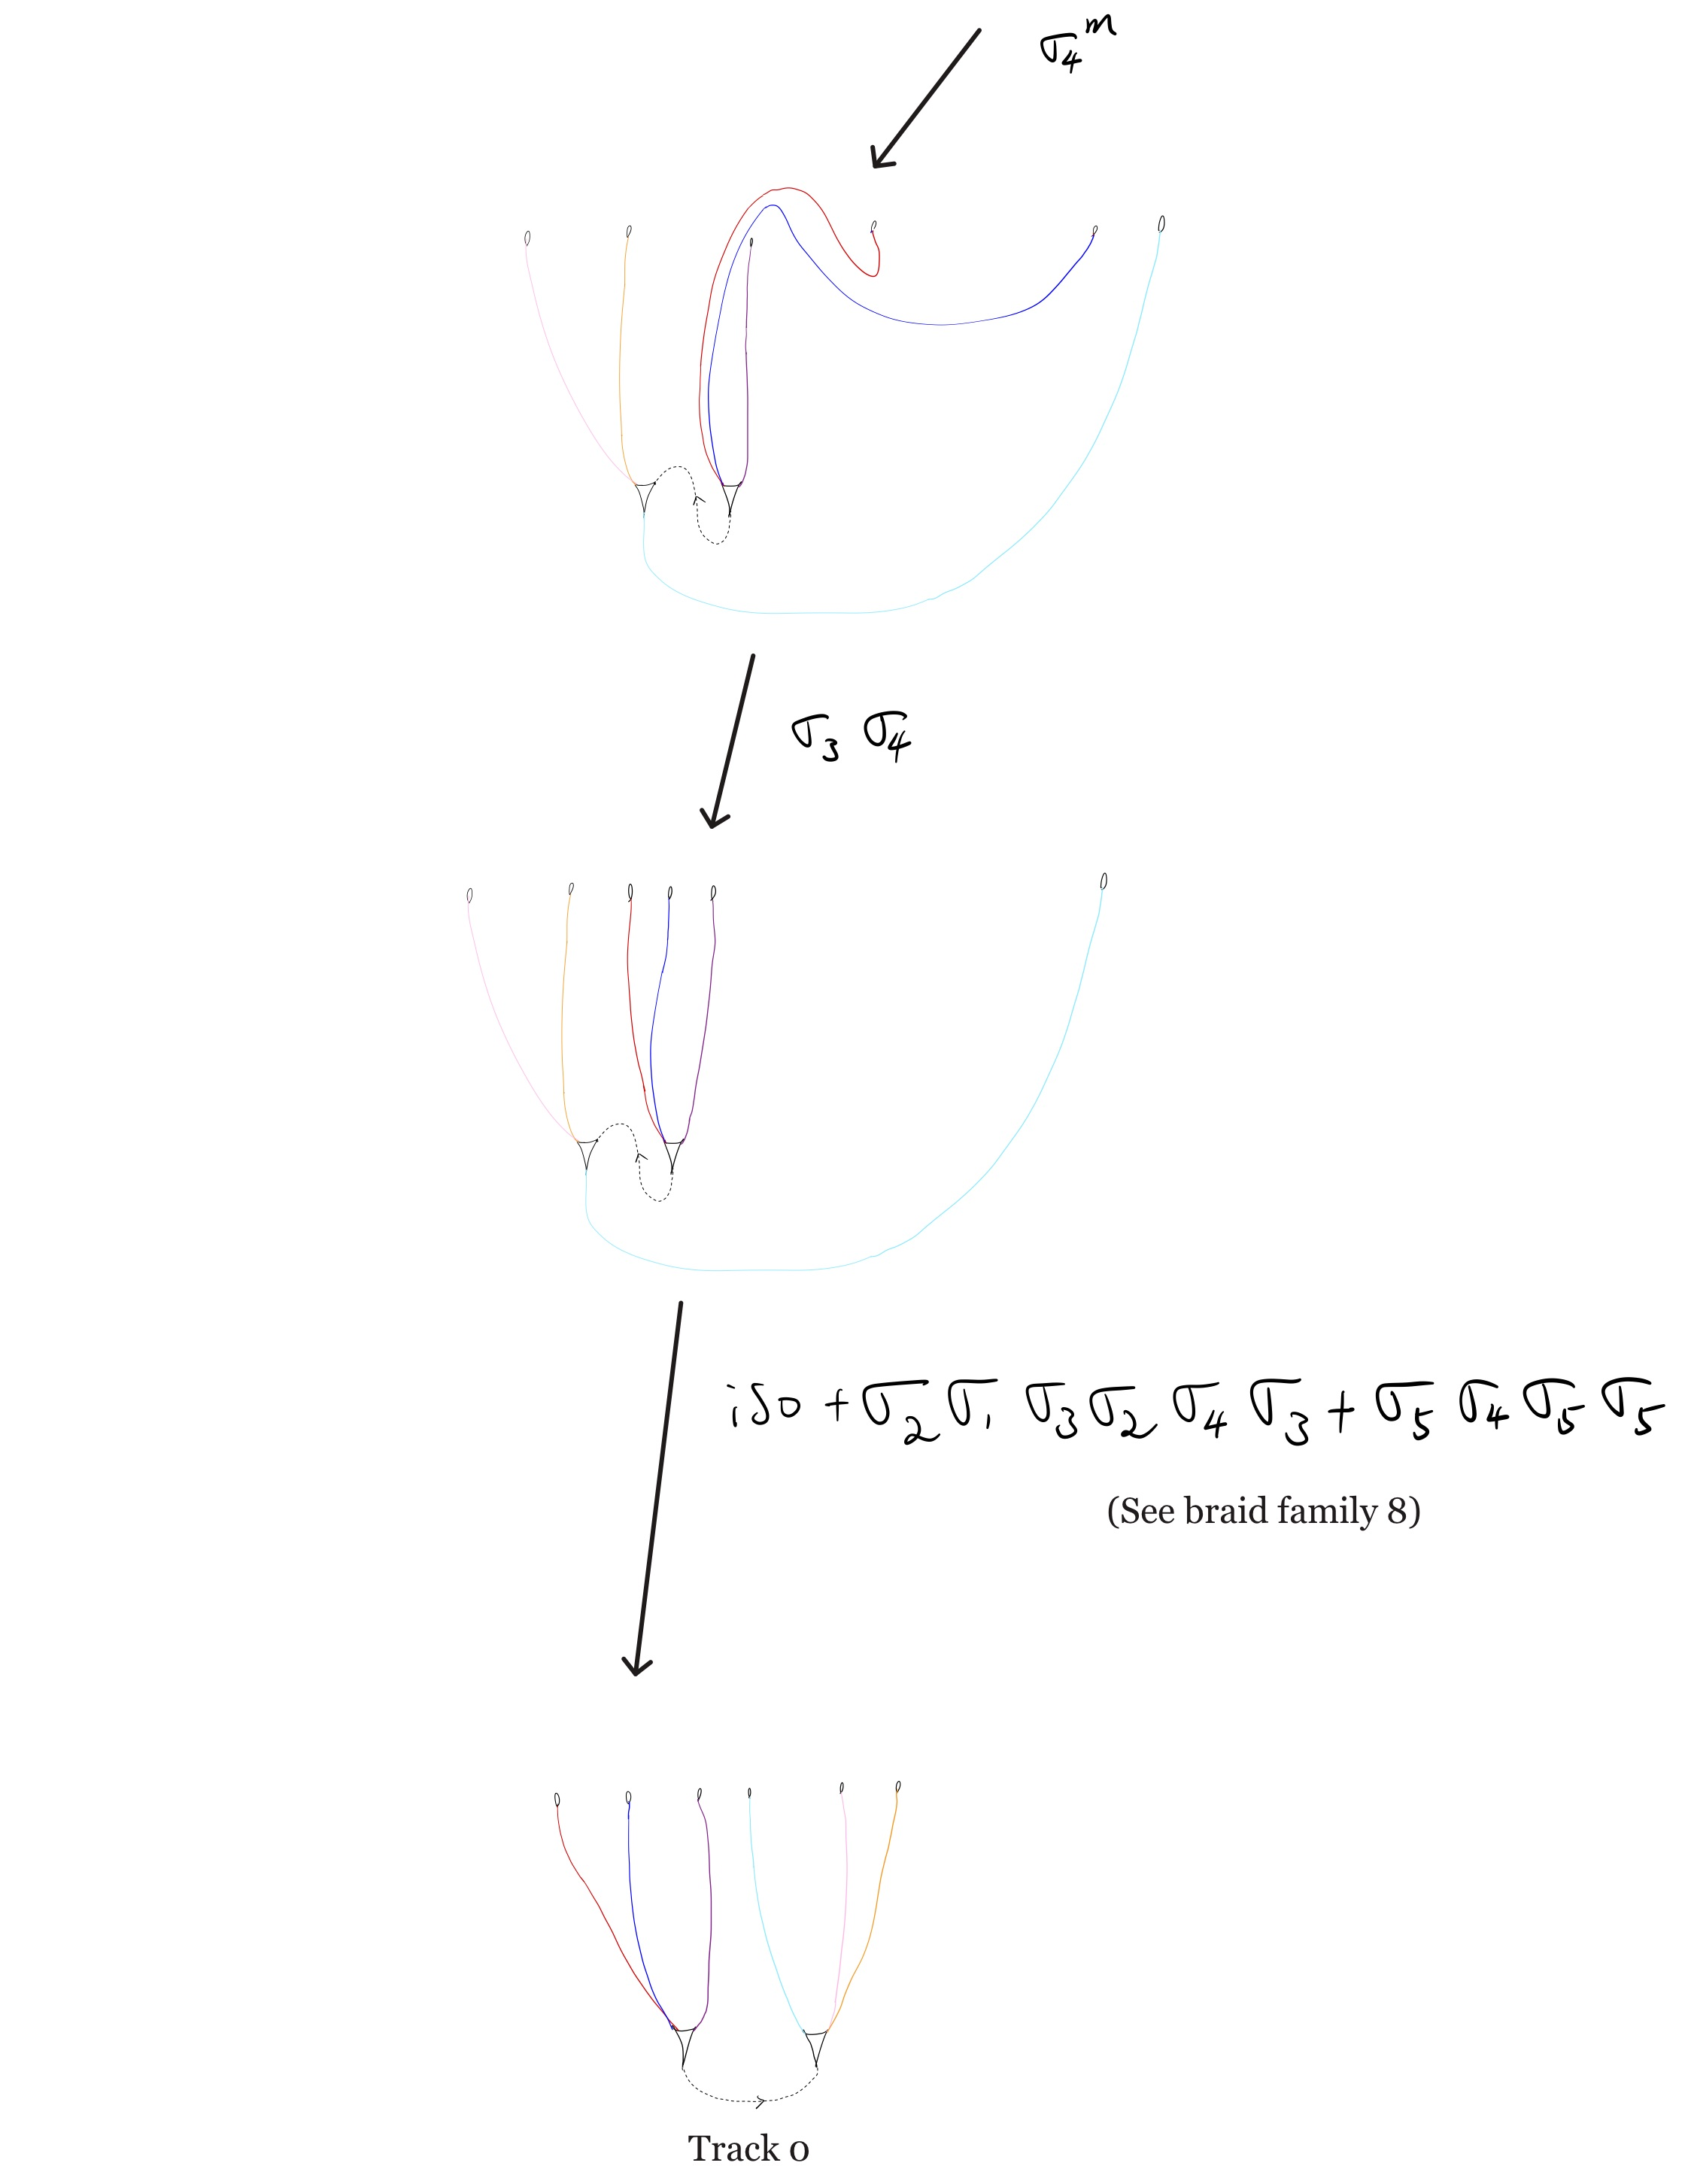
\includegraphics[width=\linewidth, height=0.45\textheight, keepaspectratio]{figures_braid/figures_track_0/Track 0 Braid 13 Treasure-3.jpg}
    \caption{This sequence shows the inverse of the braid $b_{13}^0$ carries Train Track Candidate Family 13.}
    \label{fig:track0_braid_b0_13}
\end{figure*}

\clearpage